% =====================================================================
%  main.tex —— 《四维规范场论中的纽结不变量》中译本
%  编译： xelatex main.tex （两遍，以生成目录与交叉引用）
%  底本： D. Gaiotto & E. Witten, arXiv:1106.4789v1
% =====================================================================
\documentclass[11pt,a4paper]{article}

% =====================================================================
%  preamble.tex —— 中文版《Knot Invariants from Four-Dimensional Gauge Theory》导言区
%  编译方式： XeLaTeX（推荐，ctex 自动处理中文字体）
%  英文原稿： D. Gaiotto & E. Witten, arXiv:1106.4789v1, 120 pp.
%  说明： 原稿为 JHEP 风格（jheppub），此处改为 article+ctex，
%         并保留原稿全部自定义数学宏，以确保公式逐字无损。
% =====================================================================

% ---------- 版式与字体 ----------
\usepackage[UTF8]{ctex}
\usepackage[margin=2.4cm]{geometry}

% ---------- 数学 ----------
\usepackage{amsmath}
\usepackage{amssymb}
\usepackage{amsthm}
\usepackage{bm}

% ---------- 图形与链接 ----------
\usepackage{graphicx}
\graphicspath{{figs/}}
\usepackage{xcolor}
\usepackage{longtable}
\usepackage{booktabs}
\usepackage[most]{tcolorbox}
\usepackage{hyperref}
\hypersetup{
  colorlinks=true,
  linkcolor=blue!45!black,
  citecolor=green!35!black,
  urlcolor=blue!55!black,
  pdftitle={四维规范场论中的纽结不变量（中译本）},
  pdfauthor={Davide Gaiotto, Edward Witten}
}

% =====================================================================
%  原稿自定义数学宏（逐字保留；仅将 TeX 传统字体族 cmmib/eurm/eusm
%  换为 XeLaTeX 下等价的外观：粗体数学斜体 / 罗马 / 花体）
% =====================================================================
\def\t{{ \sf t}}
\def\ct{{\cmmib t}}
\def\s{{s}}
\def\be{\begin{equation}}
\def\ee{\end{equation}}
\def\bt{{{t}}}
\def\hat{\widehat}
\def\tilde{\widetilde}
\def\frak{\mathfrak}
\def\D{{\mathcal D}}
\def\MM{M_4}
\def\k{{\cmmib k}}
\def\Bbb{\mathbb}
\def\Mthree{M_3}
\def\A{{\mathcal A}}
\def\d{{\mathrm d}}
\def\tW{{W}}
\def\R{{\mathbb R}}
\def\C{{\mathbb C}}
\def\U{{\mathcal U}}
\def\CP{{\mathbb{CP}}}
\def\N{{\mathcal N}}
\def\T{{\mathcal T}}
\def\F{{\mathcal F}}
\def\Tr{{\mathrm {Tr}}}
\def\Z{{\mathbb Z}}
\def\Q{{\mathbb Q}}
\def\CC{{\mathcal C}}
\def\ad{{\mathrm{ad}}}
\def\Btriv{{\mathcal B}_{\mathrm{triv}}}
\def\L{{ L}}
\def\Bcc{{\mathcal B_{\mathrm{cc}}}}
\def\K{{\mathcal K}}
\def\V{{\mathcal V}}
\def\J{{\mathcal J}}
\def\I{{\mathcal I}}
\def\P{{\mathcal P}}
\def\B{{\mathcal B}}
\def\Boper{{\mathcal B_{\mathrm{oper}}}}
\def\NS5{\mathrm{NS5}}
\def\uD5{\mathrm{D5}}
\def\M{{\mathcal M}}
\def\W{{\mathcal W}}
\def\H{{\mathcal H}}
\def\ZZ{\eusm B}
\def\cZ{\mathcal Z}
\def\sW{{ W}}
\def\sY{{ Y}}
\def\nY{{\mathcal Y}}
\def\ca{{\cmmib a}}
\def\ss{{d}}
\def\m{\cmmib m}
\def\bar{\overline}
% ---- 字体族替代（XeLaTeX 现代等价物） ----
\newcommand{\cmmib}[1]{\boldsymbol{#1}}      % 原 cmmib10：粗体数学斜体
\newcommand{\eusm}[1]{\mathcal{#1}}          % 原 eusm10：欧拉花体
\newcommand{\eurm}[1]{\mathrm{#1}}           % 原 eurm10：欧拉罗马

% =====================================================================
%  结构化学术版式
% =====================================================================

% ---- “本节重点”方框 ----
\newtcolorbox{keytakeaways}{
  enhanced,
  breakable,
  colback=blue!3!white,
  colframe=blue!45!black,
  boxrule=0.7pt,
  arc=2pt,
  left=6pt, right=6pt, top=5pt, bottom=5pt,
  title={\bfseries 本节重点（Key Takeaways）},
  fonttitle=\small\bfseries,
  coltitle=white,
  attach boxed title to top left={yshift=-2mm, xshift=4mm},
  boxed title style={colback=blue!45!black, arc=1pt, boxrule=0pt},
  top=10pt
}

% ---- 译者按 ----
\newtcolorbox{transnote}{
  enhanced,
  breakable,
  colback=gray!4!white,
  colframe=gray!55!black,
  boxrule=0.5pt,
  arc=1pt,
  left=5pt, right=5pt, top=4pt, bottom=4pt,
  title={\bfseries 译者按},
  fonttitle=\small,
  coltitle=black,
  colbacktitle=gray!20!white,
  top=9pt
}

% ---- 行距与段落 ----
\linespread{1.08}
\setlength{\parskip}{2pt}

% ---- 图表标题 ----
\usepackage[font=small,labelfont=bf]{caption}


\begin{document}

% =====================================================================
%  frontmatter.tex —— 标题页、摘要、译者说明
% =====================================================================
\title{\bfseries 四维规范场论中的纽结不变量\\[6pt]
       \large Knot Invariants from Four-Dimensional Gauge Theory}
\author{Davide Gaiotto$^{1}$ \quad Edward Witten$^{1,2}$\\[4pt]
        \small 中译：学术翻译工作稿}
\date{arXiv:1106.4789v1 [hep-th]，2011 年 6 月 23 日}
\maketitle

\begin{center}
\small
$^1$School of Natural Sciences, Institute for Advanced Study,\\
1 Einstein Drive, Princeton, NJ 08540 USA\\
$^2$Department of Physics, Stanford University, Palo Alto, CA 94305
\end{center}

\vspace{1em}

\begin{abstract}
\noindent
已有论证表明，基于电磁对偶及其他要素，三维中纽结的 Jones 多项式可以通过计数四维中某些规范场方程的解来计算。本文试图不借助任何量子对偶性，直接分析这些方程并计数其解，以验证这一结果。在对这些方程作适当扰动、使其行为更为一般之后，我们能够相当清楚地理解 Jones 多项式是如何浮现的。论证的主要要素，是所讨论的四维规范场方程与二维 Virasoro 代数退化表示的共形块之间的联系。在此过程中，我们对该主题与数学物理中众多新旧课题的关联获得了更好的理解——从 Gaudin 自旋链的 Bethe 拟设，到 BPS 单极子的 $M$ 理论描述，再到 Chern-Simons 规范理论与 Virasoro 共形块之间的关系。
\end{abstract}

\newpage

\vspace{0.5em}

\begin{transnote}
\textbf{关于本译稿。}
\begin{itemize}\setlength{\itemsep}{2pt}
\item \textbf{底本}：英文原稿 D. Gaiotto, E. Witten, \emph{Knot Invariants from Four-Dimensional Gauge Theory}, arXiv:1106.4789v1（120 页，含 29 幅图）。译文以原稿的 \LaTeX{} 源码为底本进行语义级翻译，\emph{全部数学公式逐字保留原文}（仅译出 \verb|\text{...}| 中的说明性文字），因此公式与原稿严格一致；若原稿存在笔误或记号歧义，均以 \verb|% [Tutor Note: ...]| 的形式在源码中就地标注。
\item \textbf{术语}：遵循中文理论物理界约定（规范场论、和乐、反常、共形块、算符乘积展开等）；人名、理论名与数学专名（Jones, Khovanov, Witten, Nahm, oper, thimble 等）保留原文。
\item \textbf{图表}：原 PDF 中的 29 幅图已逐幅裁剪为位图，存于 \verb|figs/| 目录，并在正文对应位置以 \verb|figure| 环境插入；图注中标注了原稿页码，便于对照。
\item \textbf{批注}：正文关键推导处嵌有 \verb|% [Tutor Note: ...]| 形式的学术批注（易错点预警、作者省略的证明、约定差异、原文疑似笔误等），供研读时参考；这些批注不影响编译产物。全部批注另汇编为随稿交付的 \verb|审校批注汇编.md|，按章节顺序排列，便于检索。
\item \textbf{编译}：XeLaTeX（\verb|ctex| 宏包）编译；源码缩进与分段已整理，可直接增删修改。
\end{itemize}
\end{transnote}

\vspace{0.5em}
\noindent\textbf{记号约定速查}\quad
$G$：本文重点研究的“磁”描述中的规范群；$G^\vee$：Chern-Simons 描述中的规范群（与原文 \cite{fiveknots} 的记号相反）；
$\t$：BPS 方程中的实参数，取值于 $\mathbb{RP}^1$；
$b^\pm$：二形式 $b$ 的自对偶/反自对偶投影；
$\d_A$：规范协变外微分；$\Tr$：规范群伴随表示上的迹。
上述约定与原稿一致，阅读时请特别注意 $\t$ 的特殊地位——它并非耦合常数，而是方程族的一个形变参数，$\t=1$ 与一般 $\t$ 的物理差异是全文的一条主线。

\newpage
\tableofcontents
\newpage


% ---------------- 正文（按原稿章节顺序） ----------------
\section{引言}

\begin{keytakeaways}
\begin{itemize}\setlength{\itemsep}{2pt}
  \item \textbf{物理图像}：Jones 多项式来自三维 Chern-Simons 型拓扑理论，Khovanov 同调来自四维拓扑理论；后者在圆上紧致化即约化为前者。因此四维的"计数椭圆方程解"应重现 Jones 多项式，而其再升一维（范畴化）应给出 Khovanov 同调。
  \item \textbf{数学工具}：N=4 超 Yang-Mills 理论中的 BPS 方程 (\ref{bpseqns})、Nahm 方程与 Nahm 极边界条件、主嵌入与正则元素、瞬子数、GNO/Langlands 对偶群。
  \item \textbf{主要结论}：配分函数由带符号地计数 BPS 方程的解给出（式~(\ref{partfn})）；当 W 取三维欧氏空间、对偶群取 SU(2) 且纽结标以二维表示时，它应成为 Jones 多项式。
  \item \textbf{方法要点}：沿 $x^1$ 方向拉伸纽结以实现三维约化，再用参数的绝热演化拼回四维图像；并借助库仑分支参数破坏规范对称性，以在低能下得到阿贝尔描述。
  \item \textbf{伏笔}：五维提升只有在 $t=\pm1$ 时才具有出人意料的四维对称性，这正是本文先取 $t=\pm1$、随后又扰动 $t$ 的原因。
\end{itemize}
\end{keytakeaways}

Jones 多项式 \cite{Jones} 是纽结的一个不变量，它与数学物理的许多方面有着多重联系，包括可积格点统计力学、二维共形场论及与之相关的辫群表示，以及三维 Chern-Simons 规范理论。Khovanov 同调 \cite{Khovanov} 是较晚近的一个四维拓扑理论；在这一理论中，纽结被看作三维空间中的一个对象，而与纽结相联系的不变量是一个（物理态的）向量空间，而不是一个数。两个理论之间的关系是：与 Khovanov 同调相联系的四维理论在圆上紧致化后，约化为给出 Jones 多项式的三维理论。

Khovanov 同调已在拓扑弦的框架内得到物理解释 \cite{GSV}，其基础是关于开弦 BPS 态的早期工作 \cite{OV}。关于更多进展的示例，见 \nocite{LMV,NV,Ma,DGR,DVV,AY,CNV,ACDKV,AgS} \cite{LMV}-\cite{AgS}。文献~\cite{fiveknots} 给出了 Khovanov 同调的另一种但密切相关的物理解释，其中可以找到关于 Jones 多项式、Khovanov 同调及其与数学物理之关系的更详细文献。

按照这一较新的提议，Jones 多项式可以通过计数四维中某些椭圆偏微分方程的解来计算，而 Khovanov 同调则可以通过计数 4+1 维中相关方程的解来构造。导出这一提议的推理依赖于四维 $\N=4$ 超 Yang-Mills 理论的电磁对偶：把一个本质上相当"量子"的描述（它与包围三维流形上的 Chern-Simons 规范理论密切相关）变换为另一个"半经典"的描述，在后一描述中，配分函数只需适当地计数某些微分方程的经典解即可算出。

与其依赖电磁对偶来预言这个或许有些神秘的结果，我们能否通过对这些方程的直接研究来理解它？这就是本文的目标。我们将对 Jones 多项式获得相当程度的理解，并为理解 Khovanov 同调打下良好的基础。

\subsection{简要回顾}\label{review}

这里所说的四维方程可以描述如下。规范群是一个紧李群\footnote{我们颠倒了 \cite{fiveknots} 中的记号：把 Chern-Simons 描述中的规范群记作 $G^\vee$，而把对偶的"磁性"描述中的规范群记作 $G$，本文关注的正是后者。}   $G$。方程中的场包括一个规范场 $A$，它是 $G$-丛 $E\to \MM$ 上的联络，其中 $\MM$ 是一个有向黎曼四维流形；还包括另一个场 $\phi$，它是取值于 $G$ 的伴随表示的一形式。这些方程最初是在与几何 Langlands 对应相关的研究中提出的 \cite{KW}，它们为
\begin{align}\label{bpseqns} (F-\phi\wedge \phi + \t \,\d_A\phi)^+&=0   \cr
                             (F-\phi\wedge\phi-\t^{-1}\d_A\phi  )^- &=0 \cr
                               \d_A\star\phi&=0,                     \end{align}
其中两形式 $b$ 的自对偶与反自对偶投影分别记作 $b^\pm$；$\d_A=\d+[A,\,\cdot\,]$ 是规范协变外微分；$F=\d A+A\wedge A$ 是 Yang-Mills 场强；$\star$ 是 Hodge 星号算子；$\t$ 是一个实参数。（实际上，$\t$ 取值于 $\mathbb{RP}^1=\mathbb{R}\cup\infty$；当 $\t\to 0$ 或 $\t\to\infty$ 时，需将第二个方程乘以 $\t$，或将第一个方程乘以 $\t^{-1}$。）为研究纽结不变量，我们取 $\MM=W\times \R_+$，其中 $W$ 是一个三维流形，$\R_+$ 是半直线 $y\geq 0$（图~\ref{knotboundary}）。
% [Tutor Note: 易错点] 自对偶/反自对偶投影的符号约定为 b^± = (b ± ⋆b)/2（以 ⋆² = +1 于两形式上的黎曼度量为前提）；若采用相反的 ± 约定，式 (\ref{bpseqns}) 中 t 与 t^{-1} 的角色会互换，核对时务必回到原文定义。另注意 t 并非普通实数参数，而是射影直线 RP¹ 上的点：t→0 与 t→∞ 处的方程须分别乘以 t 或 t^{-1} 才能取到有限的极限，直接令 t=0 会丢失一个方程。

\begin{figure}
 \begin{center}
     % >>> 原文图 1（原稿第 5 页）
  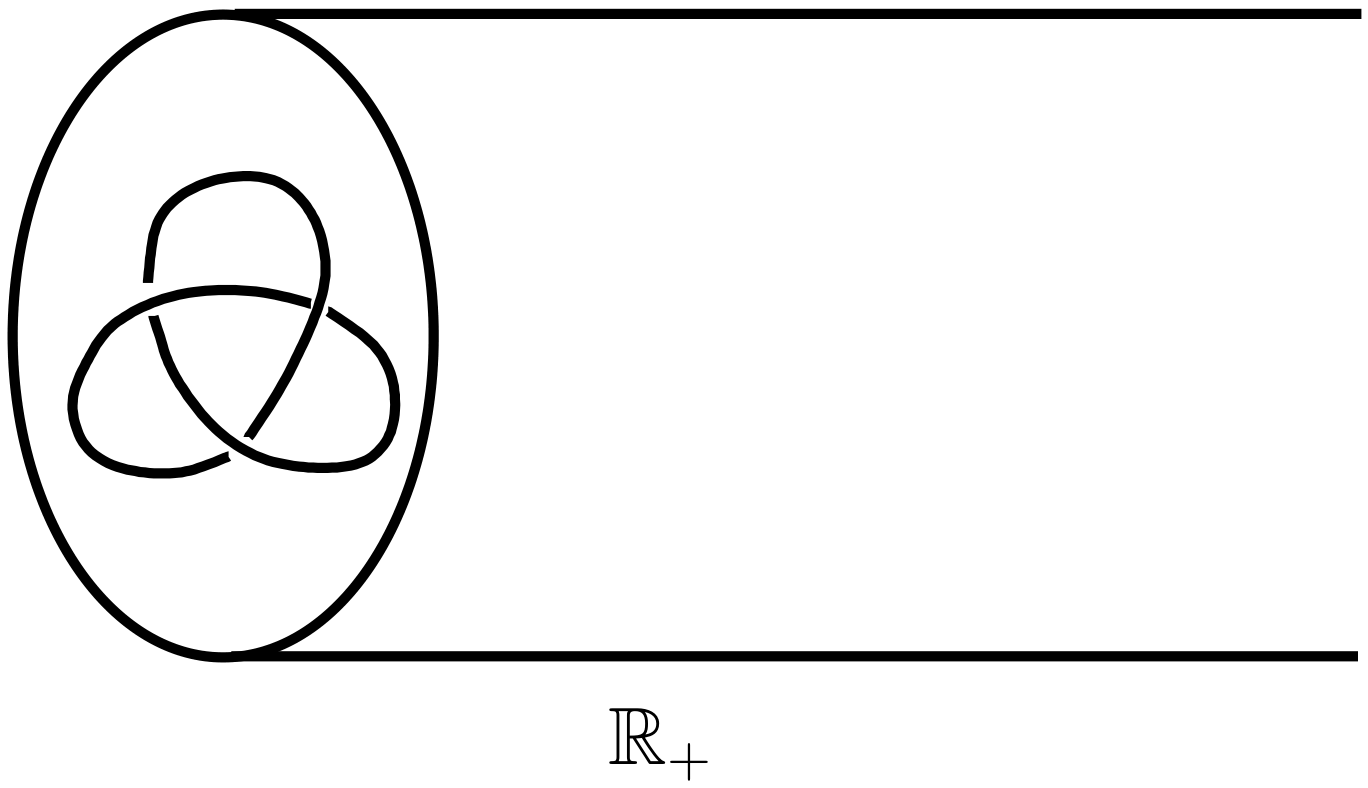
\includegraphics[width=3.5in]{figs/Fig01.png}
 \end{center}
\caption{\small  一个纽结被置于四维流形 $\MM=W\times\R_+$ 的边界上。（原稿第 5 页）}
 \label{knotboundary}
\end{figure}



$y=0$ 处的边界条件略显微妙，但在没有纽结的情形下可以很容易地描述。先假设 $\t=1$。由于边界条件是局域的，我们在描述它时不妨取 $W=\R^3$。（无论如何，这正是本文的主要例子。）考虑一个在沿 $\R^3$ 的平移下不变、且 $A$ 与 $\phi$ 垂直于边界的分量均为零的经典解。此时方程约化为关于 $\vec\phi$——即 $\phi$ 与边界相切的部分——的 Nahm 方程：
\begin{equation}\label{nahm}\frac{\d \vec\phi}{\d y}+\vec\phi\times \vec\phi = 0. \end{equation}
这些方程有一个奇异解，最初由 Nahm 在其关于磁单极子的工作中引入。取一个嵌入  $\rho:\frak{su}(2)\to \frak g$（其中 $\frak{su}(2)$ 与 $\frak g$ 分别是 $SU(2)$ 与 $G$ 的李代数），它由满足 $[\ct_1,\ct_2]=\ct_3,$ 及其循环置换的三元元素 $\vec \ct\in \frak g$ 给出。于是解为
\begin{equation}\label{nahmpole}\vec\phi=\frac{\vec \ct}{y}. \end{equation}
虽然任何 $\rho $ 都给出一个解，但我们所需的情形是 $\rho$ 为主嵌入。对 $G=SU(N)$，这意味着 $\rho$ 是 $SU(2)$ 在 $G$ 中的不可约嵌入；对一般的 $G$，这意味着升算符 $\ct_+=\ct_1+i\ct_2$ 是复化李代数 $\frak g_\C$ 的"正则"元素（即 $\frak g_\C$ 中与 $\ct_+$ 对易的子代数的维数达到最小可能值）。于是可以通过只保留那些在 $y\to 0$ 时可由带正则 Nahm 极的模型解 (\ref{nahmpole}) 逼近的解 (\ref{bpseqns})，来定义一个边界条件。这一点对任何 $\t$ 都有类似物；如附录中所述，其出发点是把规范场的切向部分 $\vec A$ 取为 $\vec\phi$ 的某个特定倍数，使方程再次约化为 Nahm 方程。
% [Tutor Note: 易错点] 模型解 φ = c/y 在 y→0 处发散，因此"用模型解逼近"指的是渐近展开的首项，而不是在 y=0 处取值；边界条件实际施加于 y→0 的渐近行为。又，"正则元素"的条件（中心化子维数最小）在 G=SU(N) 时恰好排除非主嵌入，这是把任意嵌入 ρ 限制为主嵌入的数学表述。注意此处的李代数记作 g、复化为 g_C，与对偶群 G^∨ 的记号要分清。

当包含一个链环 $L\subset W$ 时，这一边界条件沿 $L$ 被修改。链环就是互不相交的嵌入圆 $K_i$ 的并 $L=\cup_iK_i$。每个 $K_i$ 由 $G$ 的 Langlands 或 GNO 对偶群 $ G^\vee$ 的表示 $R^\vee_i$ 标记，而在此描述中，纽结仅通过它们进入边界条件的方式进入形式体系。粗略地说，这一修改要求沿 $K_i$ 存在奇异的 BPS 磁单极子，其磁荷由 $R^\vee_i$ 给出。
% [Tutor Note: 物理图像] 这是全文的关键结构：纽结不出现在四维方程本身，而只出现在 y=0 边界条件的奇点中。磁荷由对偶群的表示 R^∨ 标记，故"用哪个表示"对应"Chern-Simons 一侧插入哪条 Wilson 线"；G 与 G^∨ 的这种分工与几何 Langlands 对偶中的对偶群一致，核对时勿把 R^∨ 误写成 R。

$G$-丛 $E\to \MM$ 有一个按通常方式定义为 $\int_{\MM}\Tr\,
F\wedge F$ 的倍数的瞬子数 $P$。（把 $P$ 定义为拓扑不变量涉及一些微妙之处，\cite{fiveknots} 中有相应描述；粗略地说，$\R_+$ 的有限端与无限端的边界条件给出 $E$ 的适当平凡化，从而使瞬子数得以定义。\footnote{对
 一般的 $W$ 以及 $y=\infty$ 处边界条件的一般选取，$P$ 的取值不在 $\Z$ 中，而在 $\Q$ 中 $\Z$ 的某个陪集里。}）对瞬子数的每个取值 $n$，通过"计数"（带符号，符号由 $\N=4$ 超 Yang-Mills 理论费米子行列式的符号决定）瞬子数为 $n$ 的超对称方程 (\ref{bpseqns}) 的解的数目，可以定义一个整数 $a_n$。于是某个版本的扭化 $\N=4$ 超 Yang-Mills 理论在 $\MM$ 上的配分函数为
\begin{equation}\label{partfn} Z(q)=\sum_n a_nq^n, \end{equation}
其中 $q$ 用 $\N=4$ 超 Yang-Mills 理论参数的定义已在 \cite{fiveknots} 中说明。
% [Tutor Note: 约定差异] 此处的"计数"是带符号的（受费米子行列式符号支配），并非简单数解；若只数解的个数，得到的将是 q 取某极限时的退化形式。另外瞬子数 P 的量子化在一般 W 上并不落在整数格 Z 中，而在 Q 中 Z 的某个陪集里（见脚注），这会影响 q 的幂次是否为整数，进而影响配分函数的单值性，是后文讨论 q^{1/4} 等因子的伏笔。

为得到 Jones 多项式及其对其他群与表示的类似物，我们取 $W=\R^3$，并把 $y=\infty$ 处的边界条件简单地取为 $A,\phi\to 0$。于是，例如当 $G^\vee=SU(2)$ 且 $R^\vee$ 为 $SU(2)$ 的二维表示时，$Z(q)$ 应当成为 Jones 多项式。由于 $W=\R^3$ 正是与 Jones 多项式相关的情形，它将成为本文的主要例子。然而，我们的许多考虑也适用于 $W=\R\times C$（其中 $C$ 是黎曼面）的情形，因此我们也将考虑这一情形。

对上述程序的一个小推广是修改无穷远处的边界条件，使 $A$ 与 $\phi_y$ 为零，而 $\vec\phi$ 在相差一个规范变换的意义下趋于 $\frak t$（$G$ 的极大环面 $T$ 的李代数）中指定的三元元素 $\vec \ca$。物理上，这意味着把无穷远处的真空取为库仑分支上一个给定点所指定的真空。（在存在 Nahm 极边界条件时，开启 $\phi_y$ 或 $\N=4$ 超 Yang-Mills 理论的另外两个标量场——在 \cite{fiveknots} 中记作 $\sigma,\bar\sigma$——会破坏超对称；因此 $\vec \ca$ 是唯一有用的库仑分支参数。）连续地开启库仑分支参数应当不会影响椭圆方程解的计数，所以这一程序应当给出计算 Jones 多项式的略微更一般的方法。为描述在无穷远处取定 $\vec \ca$ 时方程 (\ref{bpseqns}) 的基本解，我们寻找仍然满足 $A=\phi_y=0$、仍然在沿 $\R^3$ 的平移下不变，但如今满足 $\lim_{y\to\infty}\vec\phi = g \vec \ca g^{-1}$（对某个 $g\in G$）的解。方程仍然约化为 Nahm 方程 (\ref{nahmpole})。一个一般性定理 \cite{Krontwo} 指出：对任何单李群 $G$ 以及 $\vec \ca$ 的任何指定选取，存在唯一的 Nahm 方程解，它在 $y=0$ 处有正则 Nahm 极，并在 $y\to \infty$ 时具有所要求的行为。该解描述了在边界上没有 't Hooft 算符时，库仑分支上给定点处的基态。
% [Tutor Note: 原文笔误] 此处"方程仍然约化为 Nahm 方程 (\ref{nahmpole})"所引的标签指向的是解 φ = c/y，而 Nahm 方程本身是式 (\ref{nahm})；按上下文 (\ref{nahmpole}) 疑为笔误。译文按原文保留 \ref 参数未改，读者应参阅式 (\ref{nahm})。

\subsubsection{提升到 Khovanov 同调}\label{lift}

尽管我们的主要关注点是从这一框架中恢复 Jones 多项式，我们也将简要勾勒 Khovanov 同调应当如何出现。这样做的一个主要目的，是说明 $\t=\pm 1$ 这些特定取值在多大程度上是特殊的、又在多大程度上不是，因为这一点在后文中很重要。

为得到 Khovanov 同调而非 Jones 多项式，我们应当把上述情形"范畴化"，这不过是说：我们必须从更高一维的理论中获得迄今所描述的一切。为此，设 $x^1,x^2,x^3$ 为 $W$ 上的局部坐标，并把 $\phi$ 分解为 $\phi =\vec\phi\cdot \d\vec x+\phi_y \d y$，其中 $\phi_y$ 是 $\phi$ 沿 $y$ 方向的分量。范畴化通过引入一个新的时间坐标 $x^0$ 并用协变导数 $D/D x^0$ 替代 $\phi_y$ 来实现。这一替代是合理的，因为 $\phi_y$ 在 (\ref{bpseqns}) 中只出现在对易子与协变导数内部，所以该替代确实给出一个微分方程（而非微分算子），如今定义在五维流形 $\R\times W\times \R_+$ 上。此外，这个微分方程（其细节见 \cite{fiveknots} 第 5 节）是椭圆的，因此计数其解的问题是有意义的。\footnote{该方程也已在 \cite{Haydys} 中得到表述，并描述了某些基本性质。}

四维方程 (\ref{bpseqns}) 的这一五维提升，在取 $\t=\pm 1$ 时还具有出人意料的四维对称性。原本关联 $\MM=W\times\R_+$ 中不同方向的四维对称性，已被替代 $\phi_y\to D/D x^0$ 所破坏。但在 $\t=\pm 1$ 时，五维方程获得了一种新的四维对称性：可以把 $\R\times W$ 替换为一般的有向黎曼四维流形 $M$（无需额外的结构），并在 $M\times \R_+$ 上表述这些方程。对研究 Jones 多项式而言，$\t=\pm 1$ 这些取值并不特别突出；椭圆方程 (\ref{bpseqns}) 解的计数与 $\t$ 无关。此外，范畴化——即替代 $\phi_y\to D/D x^0$——并不限于 $\t=\pm 1$。$\t=\pm 1$ 的特殊之处在于范畴化理论具有四维对称性，而这很可能对 Khovanov 同调及其在其他流形上的类似物有重要含义。
% [Tutor Note: 含糊点拨] 作者在此把"t 无关"与"t=±1 的四维对称性"分开陈述，容易被误读为矛盾：计数解的数目的确不随 t 变，但范畴化后保持超荷 Q 所需的流形结构随 t 改变——只有 t=±1 时 Q 只依赖 M 的黎曼结构，其他 t 需要 M 上额外的复结构。这一点是后文讨论"何时可把四维结果搬到一般四维流形"的根据。

从物理的观点看，方程 (\ref{bpseqns}) 的五维提升是某个扭化版本的五维超 Yang-Mills 理论在 $\R\times W\times \R_+$ 上的 BPS 条件；它们描述在其中一个超荷（我们称之为 $Q$）下不变的位形。该算符满足 $Q^2=0$，而超对称基态的空间就是 $Q$ 的上同调。这就是 Khovanov 同调的候选者。数学上，这些五维方程可以解释为 Morse 理论的流方程，而超对称基态的空间则是此情形下 Floer 同调的类似物。物理上，为构造超对称基态的空间，我们从五维方程的时间无关解出发——这些解正是四维中原来的未范畴化方程 (\ref{bpseqns}) 的解。在任意一个这样的解附近展开，可以构造一个近似的超对称态；在经典近似下，这些态构成超对称态空间的一组基。然后，通过考虑经典真空之间的隧穿来计算量子修正；隧穿事件是完整的五维方程的解。

从这个观点看，Khovanov 同调与 Jones 多项式之间的联系来自如下事实：为 Khovanov 同调的经典近似提供基的那些经典解，正是计算 Jones 多项式时必须计数的那些解。

\subsection{本文所使用的方法}\label{methods}


{\it A priori}，计数非线性偏微分方程 (\ref{bpseqns}) 的解是一个令人生畏的问题。我们简化这一问题的尝试基于三个想法。

\begin{figure}
 \begin{center}
     % >>> 原文图 2（原稿第 9 页）
  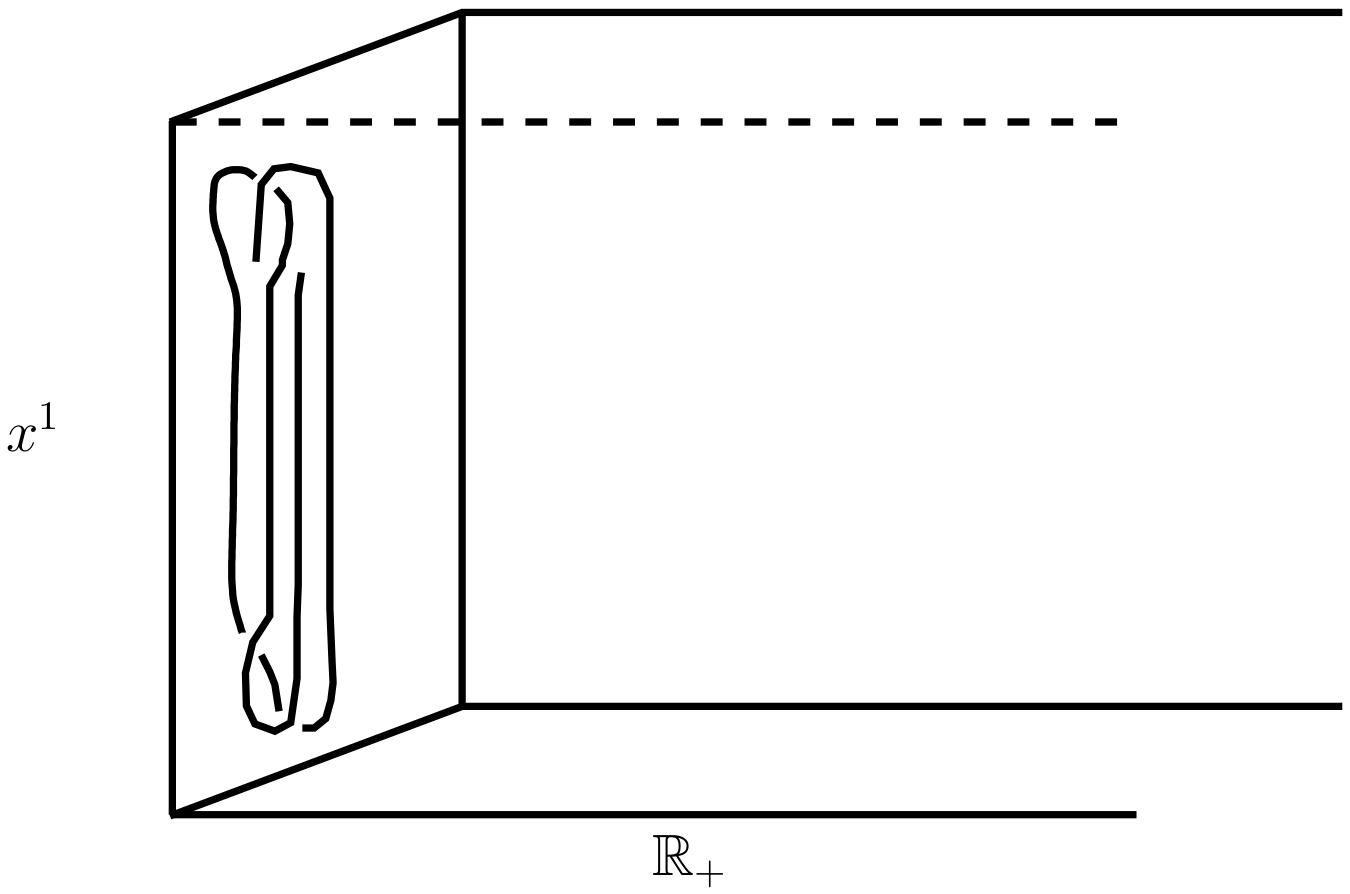
\includegraphics[width=3.5in]{figs/Fig02.png}
 \end{center}
\caption{\small   把一个纽结沿某一个方向——此处取为 $x^1$ 方向——拉伸，以约化为几乎处处近似与一个坐标无关的情形。经过充分拉伸之后，纽结处处近似与 $x^1$ 无关，唯一的例外是 $x^1$ 的有限个临界值附近，在那些地方一对股出现或消失。（在图中，这些只发生在顶部与底部。）（原稿第 9 页）}
 \label{stretching}
\end{figure}



第一个想法是拓扑场论中的标准想法。我们考虑 $W=\R\times C$ 中的纽结，其中 $C$（可以就是 $\R^2$）是一个二维流形，并用 $x^1$ 参数化 $\R$。我们把纽结沿 $x^1$ 方向拉伸，使得除了少数几个股数发生变化的例外 $x^1$ 值之外，边界条件几乎与 $x^1$ 无关（图~\ref{stretching}）。我们希望，在远离例外 $x^1$ 值的地方，解可以用与 $x^1$ 无关的解来逼近。一旦丢掉 $x^1$，方程就约化为三维中的方程。约化后的方程保持更多的超对称，人们可以期望理解它们的解。


\begin{figure}
 \begin{center}
     % >>> 原文图 3（原稿第 9 页）
  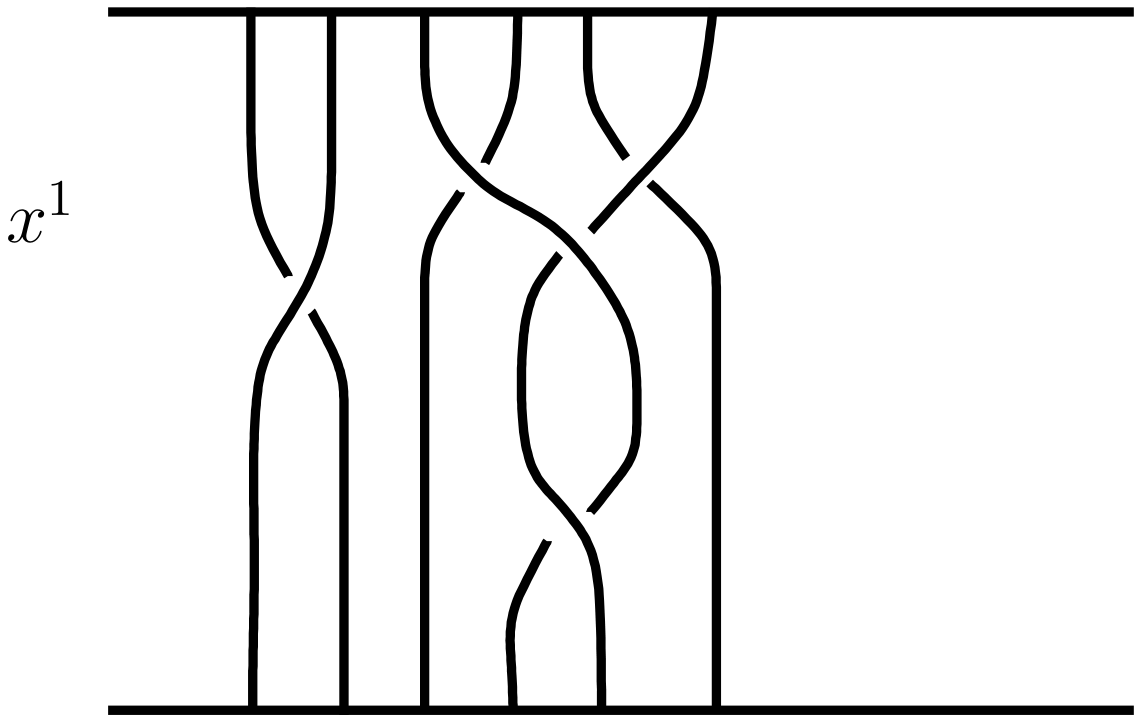
\includegraphics[width=3in]{figs/Fig03.png}
 \end{center}
\caption{\small  $I\times C$ 中的一个辫；把顶部与底部粘合起来，便可在 $S^1\times C$ 中得到一个闭合辫。经过充分拉伸后，一个辫可以用 $x^1$ 方向的绝热演化来描述，而不再有使这一描述失效的例外值。（原稿第 9 页）}
 \label{braid}
\end{figure}


在找到三维解之后，为恢复四维图像，我们必须考虑三维方程中参数的绝热变化。这是因为我们的纽结即使在拉伸之后也并非完全与 $x^1$ 无关。我们还必须考虑股数变化时发生的跳变。实际上，存在一个重要的特殊情形，其中只需考虑参数的绝热变化。这就是（图~\ref{braid}）把 $\R\times C$ 替换为  $S^1\times C$（或 $I\times C$，其中 $I$ 是闭区间，不过这会引入关于边界条件的问题）且把链环替换为辫的情形。在这种情况下，人们研究的将不是 Jones 多项式，而是与之相伴的辫群表示，后者同样极有意义。


\begin{figure}
 \begin{center}
     % >>> 原文图 4（原稿第 10 页）
  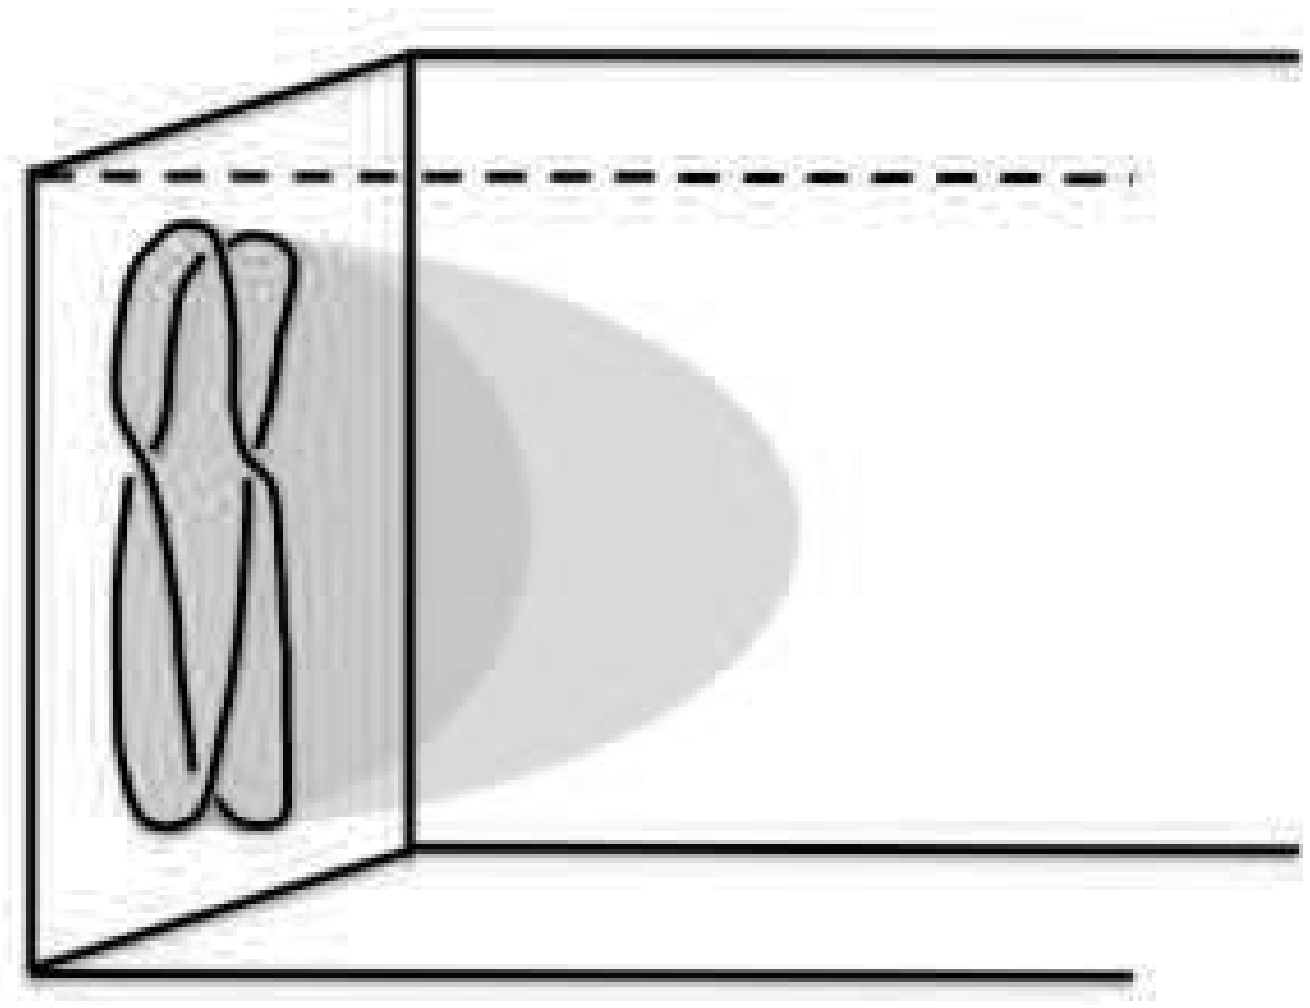
\includegraphics[width=3.5in]{figs/Fig04.png}
 \end{center}
\caption{\small  当纽结沿边界被拉伸时，超对称方程的解可能在垂直于边界的 $y$ 方向上变得离域化。图中示意性地表明了这一点；阴影区域表示解的空间延展范围——即该选定的解显著偏离无纽结时描述真空的解的区域——其厚度正比于纽结被拉伸的量。（原稿第 10 页）}
 \label{failure}
\end{figure}


关于这一方案，有一点重要之处需要提及：并不能保证它一定奏效。当把纽结沿 $x^1$ 方向拉伸时，解可能同时在 $y$ 方向上"铺展开"（图~\ref{failure}），以致即使在拉伸之后，解也可能不趋于与 $x^1$ 无关的极限。事实上，我们将发现这在某些条件下确实会发生。我们的主要任务之一，就是理解在什么条件下图~\ref{failure} 所暗示的那类行为不会发生。
% [Tutor Note: 物理图像] "铺展开"是本文的实质性困难：沿 x¹ 拉伸使边界条件的 x¹ 依赖变弱，但解在法向 y 上的尺度可能随拉伸而增大，从而不存在严格的 x¹ 无关极限。后文正是通过引入库仑分支参数破坏规范对称性、再把纽结放大到远大于 1/|a| 的尺度，来把 y 方向尺度压住；读者应把图~\ref{failure} 记作后文技术条件的直观来源。

在实施刚刚描述的方案时，我们从第~\ref{teqone}~节开始，取 $\t=\pm 1$，因为这对 Khovanov 同调是特殊取值（正如我们在上文第~\ref{lift}~节中所回顾的），也因为 $\t=\pm 1$ 时三维方程中的某些简化已在 \cite{fiveknots} 第 3.6 节中发现。

由于我们遇到了一些令人困惑的现象（最终我们将沿图~\ref{failure} 的思路理解它们），我们寻找一些额外的简化。在此过程中，我们主要利用两个想法。

第一个想法是修改边界条件以纳入规范对称性破缺。基本想法已在第~\ref{review}~节末尾解释过：我们不要求 $\vec\phi$ 在无穷远处为零，而要求 $\vec\phi\to g\vec \ca g^{-1}$，其中 $g\in G$，且 $\vec \ca=(\ca_1,\ca_2,\ca_3)$ 的三个分量取值于 $G$ 的李代数 $\frak g$ 的一个嘉当子代数中。（在更一般的情形 $W=\R\times C$ 中，我们会类似地修改边界条件，要求 $\phi$ 沿 $\R$ 方向的分量在无穷远处属于指定的共轭类。）以这种方式连续改变边界条件，应当不会改变导致 Jones 多项式的解的计数。另一方面，在此类计数问题中人们常发现，扰动到更一般的情形可以使问题变得更容易。此外，在目前的情形中，取 $\vec \ca$ 为一般的，会把我们所研究的非阿贝尔规范理论在低能下约化为阿贝尔理论。若我们把纽结放大，使 $K_i$ 的所有相关尺度都远大于 $1/|\vec \ca|$，那么我们有理由期望找到关于相关现象的某种有效阿贝尔描述。

第二个想法或许更加显然。由于在 $\t=1$ 时出现的、带上述 Nahm 极边界条件的方程相当特殊，我们扰动 $\t$ 的取值和/或 Nahm 极边界条件，使之变得更为一般。事实证明这非常富有成效，尤其是与规范对称性破缺结合时。

\subsection{结构与结果}\label{results}

在第~\ref{teqone}~节中，我们分析方程 (\ref{bpseqns}) 在 $\t=1$ 时的三维约化。我们得到以带某些附加结构的希格斯丛表述的有趣描述，但也清楚地看到，图~\ref{stretching} 所暗示的方案在 $\t=1$ 时会遇到一些困难。在第~\ref{analog}~节中，我们把方程扰动到 $\t\not=1$，并发现这为理解 Jones 多项式提供了有希望得多的框架。一般 $\t$ 的方程与数学物理中的多种课题有着出人意料且有用的联系，包括被称为 Gaudin 模型的可积自旋系统的 Bethe 方程，以及 Virasoro 代数某些特殊的"退化"共形块；本文余下部分就以这些联系为基础。在第~\ref{fourd}~节中，我们讨论由支配时间无关解的参数之绝热演化来构造辫群表示的一般框架。这一一般框架略显抽象，但在第~\ref{fthimconformal}~节中我们将证明，在我们的具体问题中，它可以借助某些 Virasoro 共形块的自由场表示而变得非常具体。在第~\ref{brrep}~节中，我们详细实施这一想法。这最终使我们能够理解如何通过计数四维 BPS 方程 (\ref{bpseqns}) 的解来恢复 Jones 多项式及与之相伴的辫群表示。第~\ref{supermon}~节致力于描述可用于理解第~\ref{teqone}~节与第~\ref{analog}~节某些微妙结果的、BPS 磁单极子的有效超势。在第~\ref{opbranes}~节中，我们把本文遇到的某些结构置于数学物理更宽广的语境中。三个附录补充推导的细节。
   % §1  引言
\section{在 \t=1 处的分析}\label{teqone}

\begin{keytakeaways}
\begin{itemize}\setlength{\itemsep}{2pt}
  \item \textbf{物理图像}：沿 $x^1$ 拉伸后，把纽结问题约化为三维流形 $M_3=C\times\R_+$ 上的时间无关解，这类解保持四个超荷，结构因而大为简化。
  \item \textbf{数学工具}：把约化方程写成三个微分算符的交换条件与矩映射条件；前者在复规范变换下不变，后者只在 G-规范变换下不变，于是问题化归为 Hitchin 意义上的希格斯丛上的全纯数据。
  \item \textbf{主要结论}：正则 Nahm 极边界条件给出额外结构——$E$ 上一个处处不被 $\phi$ 稳定的全纯线子丛 $L$；在 $\R^2$ 上它由条件 $s\wedge\phi s=1$ 刻画（只固定 $\phi$ 的一个矩阵元）。
  \item \textbf{推广}：奇异磁单极子由 $s\wedge\phi s$ 的零点实现，零点重数即磁荷；对 $SU(N)$ 的主嵌入，$L$ 及其 $\phi$ 的幂次张成整个 $E$，构成一个旗。
\end{itemize}
\end{keytakeaways}

\subsection{若干预备知识}\label{preliminaries}

\begin{figure}
 \begin{center}
     % >>> 原文图 5（原稿第 11 页）
  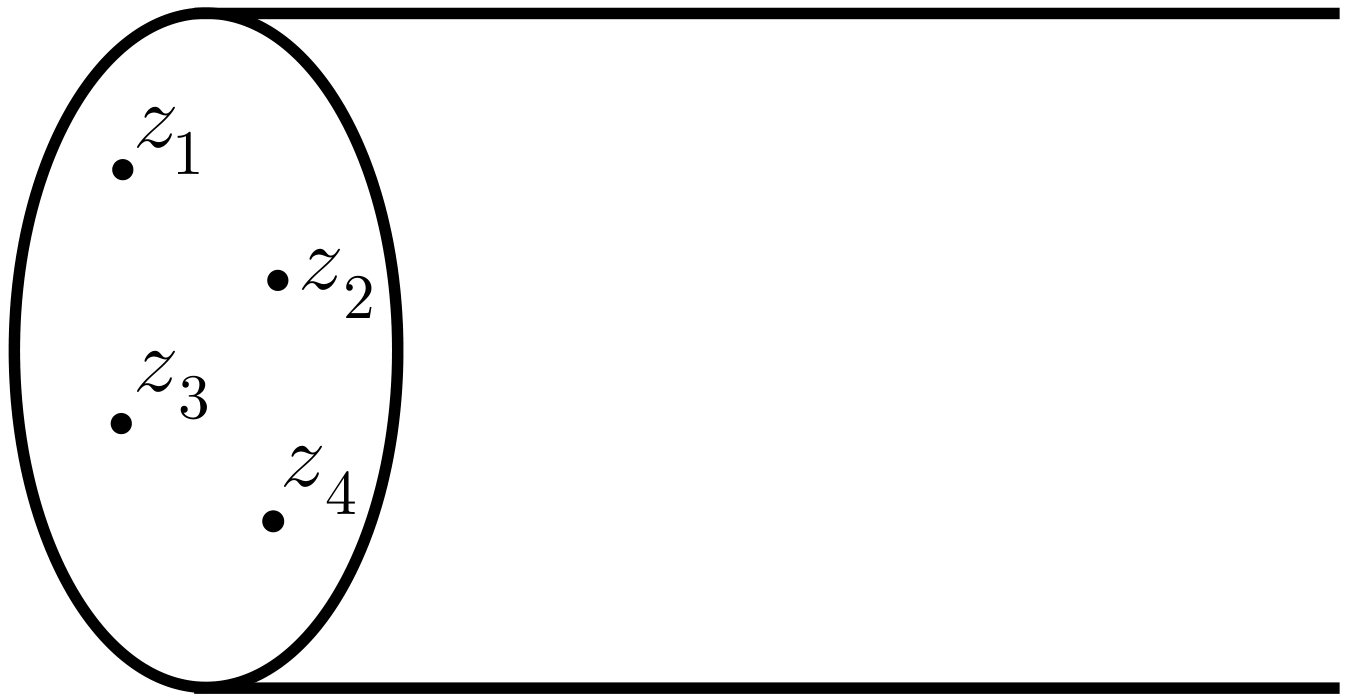
\includegraphics[width=3.5in]{figs/Fig05.png}
 \end{center}
\caption{\small  在时间无关的情形中，我们在三维流形 $M_3=C\times \R_+$ 上寻找解，其中 $C$（此处取为二维球面）是一个黎曼面。纽结被置于 $M_3$ 边界上的若干点处，此处标记为 $z_1,\dots,z_4$。（原稿第 11 页）}
 \label{redthree}
\end{figure}

正如引言中所解释的，在沿 $\MM=\R\times C\times\R_+$ 的第一个因子拉伸纽结之后，我们希望找出与第一个坐标（我们称之为 $x^1$）无关的解，也就是在三维流形\footnote{\label{confusion}
为避免混淆，我们作如下说明。本文中我们把 $\MM=\R\times C\times\R_+$ 按两种不同方式写成三维流形与一维流形的乘积：我们写
$\MM=W\times \R_+$ 而 $W=\R\times C$，但也写 $\MM=\R\times \Mthree$ 而
$\Mthree=C\times\R_+$。} $\Mthree=C\times \R_+$ 上满足约化方程的解。
这里 $C$ 是一个黎曼面（可以简单取为 $\R^2$），$\R_+$ 是半直线 $y\geq 0$。若存在纽结，我们取其支撑集为时间无关的形式 $\R\times z_i\times\{0\}$，其中 $z_i$ 是 $C$ 中的点，$\{0\}$ 是 $\R_+$ 的端点 $y=0$。图景见图~\ref{redthree}。

可由三维导出的解保持超过一般数量的超对称——确切地说，它们保持四个超荷——因此正如 \cite{fiveknots} 第 3.6 节所述，其结构会简化。在本文将会遇到的所有情形中，约化方程都可以用三个微分算符 $\D_i$（$i=1,2,3$）有效地描述。这些方程说的是：$\D_i$ 相互对易
\begin{equation}\label{commuting}[\D_i,\D_j]=0,\end{equation}
并满足矩映射条件
\begin{equation}\label{momentmap}\sum_{i=1}^3 [\D_i,\D_i^\dagger]=0,\end{equation}
其中 $\D_i^\dagger $ 是 $\D_i$ 在自然意义下的伴随。对易性约束 (\ref{commuting}) 在复值规范变换 $\D_i\to g\D_i g^{-1}$ 下不变，其中 $g$ 是取值于 $G_\C$ 的规范变换（$G_\C$ 是 $G$ 的复化）；而矩映射条件 (\ref{momentmap}) 只在取值于 $G$ 的规范变换下不变。使我们的问题变得可处理的关键在于：联立方程组的解模去 $G$-规范变换，等价于仅对易性约束 (\ref{commuting}) 的解模去 $G_\C$-规范变换。但对易性约束模去复规范变换后的解可以用全纯量来描述，因此有可能理解它们。
% [Tutor Note: 含糊点拨] 这里省略了证明，实为 Hitchin 方程/Kapustin-Witten 方程理论中的标准事实：先取 G_\C 规范把 [\D_i,\D_j]=0 化成全纯数据，再用 Hitchin 的稳定性与 Donaldson-Uhlenbeck-Yau 型定理求解矩映射，得到唯一的 G-规范等价类。此等价性并非对任意初值自动成立，前提是相应的希格斯丛满足（多）稳定性；作者在下文"我们期望可以由复规范变换求解"处再次使用了同一事实。

不同实例中的这一结构随 $\D_i$ 的构造而变，而后者依赖于 $\t$ 的选取，也依赖于我们在 $y=0$ 与 $y=\infty$ 处所设的边界条件。\cite{fiveknots} 中考虑的最基本情形是 $\t=1$（或 $-1$），且边界条件由 $\phi$ 中与边界相切的部分内的一个 Nahm 极给出。该边界条件令 $\phi_y$（即 $\phi$ 的法向部分）在 $y=0$ 处为零。若我们还要求 $\phi_y$ 在 $y\to\infty$ 时为零，则一个简单的消失性论证表明：在与 $x^1$ 无关的解中，$\phi_y$ 恒为零；类似地，$A_1$（即 $A$ 沿 $x^1$ 方向的分量）在三维解中也为零。一旦令 $\phi_y$ 与 $A_1$ 为零，方程便可写成上述形式，正如 \cite{fiveknots} 第 3.6 节\footnote{我们的记号与那里不同之处在于对坐标作了重新标号 $x^i\to x^{i+1}$（其目的是在范畴化时为新的时间坐标 $x^0$ "腾出空间"）。此外，为后文方便，我们以显然的方式置换了 $\D_i$。}中详细展示的那样，此时
\begin{align}\label{eqform} \D_1 & = \frac{D}{Dx^2}+i\frac{D}{Dx^3}    \cr
                                   \D_2 & = [\phi_2-i\phi_3,\,\cdot\,] \cr
                             \D_3 & = \frac{D}{Dy}-i[\phi_1,\,\cdot\,]  \end{align}
而矩映射条件成为
\begin{equation}\label{mmtmap}0=
\sum_{i=1}^3[\D_i,\D_i{}^\dagger]=F_{23}-[\phi_2,\phi_3]-D_y\phi_1.\end{equation}
 在写出这些公式时，我们简单地取 $C=\R^2$，坐标为 $x^2,x^3$。不过，引入复坐标 $z=x^2+ix^3$，并写 $\phi_2\d x^2+\phi_3\d x^3=\varphi \d z+\bar\varphi \d\bar z$，是有益的；我们还引入复联络 $\A_y=A_y-i\phi_1$ 用于沿 $y$ 方向的平行移动，并写 $\D_y=\d_y+[\A_y,\,\cdot\,]$。于是可以写成
\begin{align}\label{neqform} \D_1 & =2\frac{D}{D\bar z} \cr
                                                              \D_2 & = 2[\varphi,\,\cdot\,]\cr
                                                               \D_3& = \frac{\D}{\D y}. \end{align}
以这种写法，$\D_i$ 在任意黎曼面 $C$ 上都有意义，其中 $D/D\bar z$ 理解为 $\bar\partial $ 算子，$\varphi$ 为 $C$ 上的一个 $(1,0)$-形式。
% [Tutor Note: 约定差异] 与 \cite{fiveknots} 比对时须注意脚注中的坐标重标号 x^i\to x^{i+1} 以及对 \D_i 的置换；此外 z=x^2+ix^3 的选取使 \partial_z 与 \partial_{\bar z} 的归一化相差因子 2，故 \D_1=2D/D\bar z 中的系数 2 依赖于该约定。复联络写成 \A_y=A_y-i\phi_1（而非 +i\phi_1），这个符号决定了 \D_3 中与 \phi_1 的对易子项的符号，进而决定 \phi_1 与 A_y 在希格斯丛复结构中的角色。

正如保持四个超荷的几何所预期的那样，对易性约束 $[\D_i,\D_j]=0$ 可以由一个超势导出，即
\begin{equation}\label{superone}\W= \frac{1}{4\pi i}\int_{C\times \R_+}\Tr\,\varphi \F_{y\bar z},\end{equation}
其中 $\F_{y\bar z}=[\D_y,D_{\bar z}]$。更准确地说，在变分 $\W$ 以导出条件 $[\D_i,\D_j]=0$ 时，应当要求 $A$ 在 $y=0$ 处的变分为零。否则 $\W$ 的变分会包含 $y=0$ 处额外的 delta 函数项。
% [Tutor Note: 易错点] 超势变分在带边流形上会产生边界项：\delta\W 除给出 [\D_i,\D_j]=0 外，还给出正比于 \int_{y=0}\Tr(\varphi\,\delta A) 的项。只有限制 \delta A|_{y=0}=0 时，[\D_i,\D_j]=0 才恰为超势的临界条件；否则须把该边界项一并处理（这正是后文把 Nahm 极边界条件视为对变分原理的约束的原因）。

方程 $[\D_i,\D_j]=\sum_i[\D_i,\D_i{}^\dagger]=0$ 在 \cite{KW} 中被称为推广的 Bogomolny 方程；实际上，这些方程是 Nahm、Hitchin 与 Bogomolny 方程的混合体。若丢掉对 $z$ 的依赖，它们约化为 Nahm 方程；若丢掉对 $y$ 的依赖，它们约化为 Hitchin 方程；若令 $\varphi=0$，则约化为 Bogomolny 方程。这不仅仅是一个类比：我们可以借用 Nahm、Hitchin 或 Bogomolny 方程模空间理论中的标准策略。

对固定的 $y$，方程 $[\D_1,\D_2]=0$ 定义了 Hitchin 意义上的一个希格斯丛 $(E,\varphi)$。$\D_1$ 与 $\D_2$ 同 $\D_3$ 对易这一事实只意味着：在复值规范变换的意义下，该希格斯丛与 $y$ 无关。当我们特殊到 $C=\R^2\cong \C$ 时，便得到 $\C$ 上的一个希格斯丛，它可以理解为 $\CP^1=\C\cup \infty$ 上的希格斯丛，可能在无穷远处带有奇点。这一情形将在第~\ref{simvar}~节中考虑。希格斯丛的奇点还有另一种自然的产生方式。如 \cite{fiveknots} 第 6 节所述，可以纳入支撑在 $\MM$ 中余维二维子流形上的曲面缺陷。把它们取为 $\R\times q_i \times \R_+$ 的形式（其中 $q_i$ 是 $C$ 中的点），上面概括的构造仍然适用，而希格斯丛在点 $q_i$ 处获得奇点。我们在第~\ref{mondr}~节中考虑这一情形。

额外的结构来自 $y=0$ 与 $y=\infty$ 处的边界条件。我们将在第~\ref{bc}~节中讨论 $y=0$ 处 Nahm 极的后果。与 Nahm 方程的类比将会有用：对 $C$ 中的任一给定点，我们可以从对易对 $\D_2$,$\D_3$ 中提取某些全纯数据。由于 $\D_2$,$\D_3$ 与 $\D_1$ 对易，这些数据在全纯意义下（或在存在奇点时在亚纯意义下）随 $C$ 变化。

最后，与 Bogomolny 方程的类比将帮助我们理解解的物理内容，尤其是当我们在 $y\to\infty$ 时开启规范对称性破缺时。的确，对易对 $\D_1$,$\D_3$ 中的全纯数据，类似于在 Bogomolny 方程的解中指定 BPS 磁单极子位置的那些数据。

\subsection{边界条件}\label{bc}
我们的下一个任务是分析边界条件，首先在没有奇异磁单极子的情形下。$\t=1$ 时的模型解 (\ref{nahmpole}) 在 $\D_2$ 与 $\D_3$ 中有奇点，但在 $\D_1$ 中没有奇点，这仅仅是因为 $\D_1$ 不含标量场。对 $ \frak g = \frak{su}(2)$，取李代数元素 $\ct$ 的标准选取，该解显式为
\begin{equation}\label{burg}
\varphi = \frac{1}{y} \begin{pmatrix} 0 & 1 \cr 0 & 0\end{pmatrix},
\qquad A_{\bar z}=0, \qquad \A_y = \frac{1}{2y} \begin{pmatrix} 1 & 0 \cr 0 & -1\end{pmatrix}.
\end{equation}
我们在此认为这些矩阵作用在秩为二的平凡复向量丛 $E\to \R^2\times\R_+$ 的纤维上。对 $G=SO(3)$、在一般的黎曼面上，把 $E$ 定义为秩二的丛可能存在整体障碍，这时人们会转而考虑相应的伴随丛 $\ad(E)$。由于我们的考虑沿黎曼面 $C$ 是局域的，改用伴随表示重新表述不会有太大变化，我们将略过这一点。


解 (\ref{burg}) 可以写成
\begin{equation}\label{nolf} \varphi= g\varphi_1 g^{-1},
~~ \D_y=g\frac{\d}{\d y}g^{-1} \end{equation}
其中
\begin{equation}\label{zolf} \varphi_1=\begin{pmatrix} 0 & 1\cr 0 & 0 \end{pmatrix}\end{equation}
而 $g$ 是一个在 $y=0$ 处奇异的 $G_\C$ 值规范变换
\begin{equation}\label{singgauge}
g =\begin{pmatrix} y^{-1/2} & 0 \cr 0 & y^{1/2} \end{pmatrix}.
\end{equation}
换言之，该解是由平凡解 $\varphi=\varphi_1,$ $A_{\bar z}=\A_y=0$ 经复值规范变换 $g$ 得到的。

我们希望考虑在 $y=0$ 附近、在相差一个规范变换的意义下看起来像模型解的那些解。我们希望用远离边界处的希格斯丛数据 $(E,\varphi)$ 来表达这一约束。为此，考察规范丛 $E$ 的一个局部全纯截面 $s$ 在沿 $y$ 方向平行移动下不变时的行为，是有用的。我们将先对模型解非常具体地做这一计算，然后再辨认哪些特征在更一般的情形下仍然成立。

设 $s$ 是规范丛 $E$ 的一个截面，满足
\begin{equation}\label{onurf}\frac{\D s}{\D y}=0.\end{equation}
由于 $\D/\D y= g (\d/\d y) g^{-1}$，该方程的解具有 $s= gs_0$ 的形式，其中 $s_0$ 与 $y$ 无关。因此通解具有形式
\begin{equation}\label{wurf} s=\begin{pmatrix} a y^{-1/2}\cr b y^{1/2}\end{pmatrix},\end{equation}
其中 $a,b$ 为常数。特别地，$E$ 中一个一般的向量沿 $y$ 方向平行移动到 $y=0$ 时会按 $y^{-1/2}$ 发散。存在一个一维子空间，由满足 $\D s/\D y=0$ 且在 $y\to 0$ 时实际按 $y^{1/2}$ 消失的那些解组成。该子空间简单地由条件 $a=0$ 刻画。

对任意固定的 $y>0$，我们把 $E\to C\times \R_+$ 到 $C\times \{y\}$ 的限制记作 $E_y$。用 $\D_y$ 作平行移动给出所有 $y$ 的 $E_y$ 之间的自然等同，我们就把 $E_y$ 视为 $C$ 上的丛并简单地记作 $E$。类似地，$\varphi$ 到 $C\times y$ 的限制在 $\D_y$ 平行移动的意义下与 $y$ 无关。于是通过限制到 $C\times y$，我们得到希格斯丛 $(E,\varphi)\to C$。

$E$ 的"小"截面——即满足 $\D s/\D y=0$ 且在 $y\to 0$ 时消失的解 $s$——生成一个秩一子丛 $\L\subset E$。在模型解中，它简单地就是 $E$ 中形如 $\begin{pmatrix}0\cr b\end{pmatrix}$ 的截面所构成的子丛。$\L$ 是 $E\to C$ 的全纯子丛；$\L$ 的一个截面若被 $\D_1=2\,D/D\bar z$ 湮灭，则它是全纯的。具体地说，在模型解中，$\L$ 的截面 $\begin{pmatrix}0\cr b\end{pmatrix}$ 全纯当且仅当 $b$ 是 $z$ 的全纯函数。

$\L$ 全纯的根本原因在于：由于 $[\D_2,\D_3]=0$，我们可以要求 $\D_3s=0$ 的小解同时也被 $\D_2=2D/D\bar z$ 湮灭。然而，我们不能同时要求小解被 $\varphi=\D_1/2$ 湮灭。这一点从上面的公式看很清楚：在模型解中，$\varphi$ 湮灭一个向量当且仅当其下分量为零，而不是当其上分量为零。

为衡量 $\L$ 不是 $\varphi$-不变的程度，可以如下进行。若 $\L$ 是一个平凡线丛（在我们的应用中将是如此），则可选取 $\L$ 的一个处处非零的截面 $s$。对我们的模型解，只需取 $s=\begin{pmatrix} 0 \cr 1\end{pmatrix}$。然后我们定义
\begin{equation}\label{smallexp}  \kappa= s\wedge \varphi s.  \end{equation}
对模型解，我们看到 $\kappa=1$，特别地
$\kappa$ 处处非零。$\kappa$ 非零意味着 $\varphi s $ 不是 $s$ 的倍数，因此 $\L$ 不满足在乘以 $\varphi$ 下不变这一性质。
（若把 $\R^2$ 换成一般的黎曼面 $C$，可能无法选取整体非零的 $s$，但人们仍可选取 $\L$ 的一个局部截面 $s$，并通过计算 $\kappa=s\wedge \varphi s$ 来度量 $\L$ 不是
$\varphi$-不变的程度。只要 $s$ 非零，$\kappa$ 是否为零就与 $s$ 的选取无关。）

对模型解成立的三条基本性质，对任何带正则 Nahm 极的解仍然成立，因为它们不受 $y \to 0$ 时 $\D_y$ 与 $\varphi$ 的次领头行为的影响：
\begin{itemize} \item $E$ 中一个一般的向量沿 $y$ 方向平行移动到
$y=0$ 时会按 $y^{-1/2}$ 发散。 \item  那些平行移动到 $y=0$ 时实际消失的截面 $s$ 张成一个秩 1 的全纯子丛  $\L\subset E$。  \item
最后，我们不能同时要求一个小截面被 $\varphi=\D_1/2$ 湮灭。相反，在 $y=0$ 附近可由模型解逼近的解中，$\varphi$ 在 $C$ 中的任何点处都不湮灭小截面。\end{itemize}
% [Tutor Note: 物理图像] 这三条性质合起来就是"保留结构群"的图像：Nahm 极把 G_\C 结构群约化为一个抛物子群，\L 是该抛物结构中的最小子丛，\kappa=s\wedge\varphi s 则是这个抛物结构偏离 \varphi-稳定性的量度。因此"希格斯丛 + 处处非 φ-稳定的线子丛"正是 Nahm 极边界条件所编码的全纯数据，而不是任意的希格斯丛。

因此，带正则 Nahm 极（$y\to 0$）的完整方程的解所给出的并不仅仅是希格斯丛 $(E,\varphi)$。更确切地说，还存在某种额外的结构：$E$ 被赋予一个全纯线子丛 $\L$，它在任何地方都不被 $\varphi$ 稳定。在 $\R^2$ 上，$\L$ 必然是平凡的，因此我们可以简单地说：$E$ 存在一个处处非零的全纯截面 $s$，满足 $s \wedge \varphi s =1$。注意这一条件远不足以确定 $\varphi$。若 $s=\begin{pmatrix}0\cr 1\end{pmatrix}$，则条件 $s\wedge \varphi s=1$ 只固定 $\varphi$ 的右上角矩阵元，对其余矩阵元不加任何条件。之所以只固定 $\varphi$ 的一个矩阵元（用 $s$ 表示），是因为当我们作一个在 $y\to 0$ 时行为如 (\ref{singgauge}) 的规范变换时，$\varphi$ 获得的奇点只依赖于它的右上角矩阵元。在适当的情形下（亏格更高的黎曼面 $C$ 上，或在存在下面即将引入的奇异磁单极子的 $\R^2$ 上），可以存在由三元组 $(E,\varphi,\L)$ 构成的非平凡模空间，其中 $E$ 与 $\L$ 固定而只有 $\varphi$ 变化。这一点将在第~\ref{opbranes}~节中说明。

对任何三元组 $(E,\varphi,\L)$，我们期望完整方程组可以通过一个复规范变换求解。假设给定一个与 $y$ 无关的希格斯丛 $(E,\varphi)$，以及一个处处不被 $\varphi$ 稳定的全纯子丛 $\L\subset E$。在以 $\varphi s$ 与 $s$ 给出的 $E$ 的基中，我们作规范变换 (\ref{singgauge})。这将重现 $y=0$ 处的 Nahm 极奇点，但一般而言它不会给出矩映射条件 (\ref{mmtmap}) 的解。通过进一步作光滑的复规范变换，人们有望得到矩映射条件的解。
% [Tutor Note: 含糊点拨] "有望"（one can hope）背后是 Hitchin-Kapustin-Witten 的定理：给定希格斯丛若满足稳定性，则存在唯一的光滑复规范变换使矩映射为零；若不稳定，则只能得到"近似"解或需要引入额外的奇异结构。作者此处未验证稳定性条件，后文讨论库仑分支参数 \vec\ca 与纽结标号 R^\vee 的容许范围时才间接涉及这一限制，阅读时应留意。

\subsubsection{加入奇异磁单极子}\label{addsing}

为在边界处加入奇异磁单极子，我们需要用更一般的奇异解来替换 Nahm 模型解，该解见 \cite{fiveknots} 第 3.6 节。让我们考虑单个奇异磁单极子的情形，它位于 $y=z=0$。模型解在 $y\to 0$ 且 $z\not=0$ 时具有与前面相同的奇点，但在 $y=z=0$ 附近具有更复杂的形式。它可以由对易性约束的一个解经复值规范变换得到（该变换在 \cite{fiveknots} 中有明确描述），该解为
\begin{equation}\label{solcom} \varphi=
\begin{pmatrix} 0 & z^k\cr 0 & 0 \end{pmatrix}, ~~A_z=\A_y=0.
\end{equation}
为用我们现在的语言表达这一点，$\L$ 仍然由这样的截面张成：在规范 (\ref{solcom}) 中它们是
$s=\begin{pmatrix} 0 \cr 1 \end{pmatrix}$ 的倍数；这是因为 $g$ 在 $y\to 0$ 时具有与前面类似的行为。现在我们得到
\begin{equation} s\wedge\varphi s = z^k.\end{equation}
$s\wedge\varphi s$ 的零点被解释为奇异磁单极子的位置，其重数即为磁荷。这一解释立刻提示了含多个奇异磁单极子的解应当意味着什么。我们考虑由希格斯丛 $(E,\varphi)$ 及一个一般地不是 $\varphi$-不变的全纯子丛 $\L\subset E$ 所描述的解。若
\begin{equation}\label{olcomtwo} s\wedge \varphi s =\prod_{a=1}^s(z-z_a)^{k_a},\end{equation}
则我们说该解在位置 $z_a$ 处有磁荷为 $k_a$ 的奇异磁单极子。人们希望能证明：给定这样的数据，存在唯一解，它在每个 $z=z_a$ 附近的奇性与奇异模型解一致。
% [Tutor Note: 物理图像] 磁单极子的"位置"是 s\wedge\varphi s 的零点这一事实，说明奇异磁单极子并不作为独立的场存在，而是希格斯丛数据 (E,φ,L) 的奇点；电荷 k_a 即是零点重数，这也解释了为何对偶群 G^\vee 的表示 R^\vee 的维数会成为磁荷——它正是 s\wedge\varphi s 在纽结处的零点阶数。

尽管本文主要考虑 $\frak{su}(2)$，我们可以很容易地把这些陈述推广到更一般的李代数。为简单起见，取 $G=SU(N)$ 并把 $E$ 看作秩为 $N$ 的复向量丛。考虑基于 $\frak{su}(2) \to \frak{su}(N)$ 的主嵌入的 Nahm 极。$\ct_3$ 的本征空间（在 $\frak{su}(N)$ 的基本 $n$ 维表示中）是一维的，而由在 $y \to 0$ 时尽可能快地衰减的截面定义了一个线丛 $\L$。对 $\L$ 的唯一约束是：在奇异磁单极子位置之外，
\begin{equation}
 \L \oplus \varphi \L \oplus  \cdots \oplus \varphi^{n -1} \L = E
\end{equation}
当我们特殊到 $C=\R^2\cong \C$ 时，可以用 $E$ 的一个特定截面 $s$（在重新标度意义下定义）来定义线子丛 $\L$，使得截面 $s, \varphi s, \cdots,\varphi^{N-1}s$ 线性无关。这一约束在奇异磁单极子所在处按其磁荷的方式被放宽。用 $\varphi$ 的矩阵元的零点给出的等价描述见 \cite{fiveknots} 式 (3.59)。
% [Tutor Note: 原文笔误] 本段先设 G=SU(N)、E 秩为 N，但接着写"基本 n 维表示"并把分解式写成 \L\oplus\varphi\L\oplus\cdots\oplus\varphi^{n-1}\L=E；按主嵌入的维数应为 N（下文也确实写成 \varphi^{N-1}s）。原文如此，n 疑为 N 之笔误，译文未改动公式。

这可以推广到 $y=0$ 处一般 Nahm 极的情形，不必与 $\frak{su}(2)$ 的主嵌入相联系。（本文不研究这一推广。）一般地，对 $y\to 0$，存在按 $y$ 的整数或半整数幂增长的局部截面。
通过考察在 $y \to 0$ 时至多按给定幂 $y^{(n-N)/2}$ 增长的局部截面，可以在 $E$ 上定义一个全纯子丛的旗 $E_n$。显然，$E_{n+1} \subset E_n$；又有  $E_0=E$，且对足够大的 $n$ 有 $E_n=0$。乘以 $y^{-(n-N)/2}$ 后，$E_n$ 中一个一般的向量在 $y \to 0$ 时具有有限极限，而此极限是 $\ct_3$ 的、本征值为 $(N-n)/2$ 的本征向量。该映射的核为 $E_{n+1}$；因此 $y \to 0$ 的极限把商空间 $E_n/E_{n+1}$ 与 $\ct_3$ 的本征空间等同起来。乘以 $\varphi$ 给出映射 $E_n \to E_{n-2}$。由于 $\varphi \sim \frac{\ct_+}{y}$，全纯映射 $\phi_n : E_n/E_{n+1} \to E_{n-2}/E_{n-1}$ 可以等同于 $\ct_+$ 在 $\ct_3$ 的本征空间上的作用。
   % §2  在 t=1 处的分析（前半）
\subsection{无对称性破缺时的解}\label{solutions}

现在我们要用刚刚描述的想法来确定超对称方程 (\ref{commuting})、(\ref{momentmap}) 的某些解模空间。我们将对 $G=SO(3)$ 做这件事，于是用其表示来标记奇异磁单极子的对偶群是 $G^\vee=SU(2)$。

我们首先在库仑分支的原点处工作；这意味着我们考虑标量场 $\vec\phi$ 在 $y\to\infty$ 时为零的解。特别地，$\varphi$ 在无穷远处必须为零。由于方程 $\D_y\varphi=0$ 意味着 $\varphi$ 的共轭类与 $y$ 无关，$\varphi$ 只有在处处幂零时才能在无穷远处为零。这意味着通过一个复规范变换，我们可以使 $\varphi$ 成为上三角的：
\begin{equation}\label{uptri}\varphi=\begin{pmatrix} 0 & p(z) \cr 0 & 0 \end{pmatrix},\end{equation}
其中 $p(z)$ 是某个多项式。然而，我们不能同时把 $s$ 也化成标准形式。因此我们简单地取
\begin{equation}\label{nuptrix}s=\begin{pmatrix} P(z)\cr Q(z)\end{pmatrix},\end{equation}
其中 $P,$ $Q$ 是多项式。在不改变 $\varphi$ 的前提下，我们可以作一个上三角规范变换，把 $P$ 移动 $Q$ 的多项式倍：
\begin{equation}\label{uptrix} P(z)\to P(z)+U(z) Q(z).\end{equation}
除了把 $s$ 乘以一个复常数之外，这是唯一的自由度。

现在我们来问：如何选取 $p, $ $Q$, 和 $P$ 以描述边界上具有磁荷 $k_a$、位于点 $z_a$ 的奇异磁单极子的位形？由于 $s\wedge \varphi s = pQ^2$，我们需要的条件是
\begin{equation}\label{factors}
p(z) Q(z)^2 = \prod_a(z - z_a)^{k_a} := K(z).
\end{equation}
若所有奇异磁单极子都带最小磁荷 $k_a=1$，我们只能以 $p=K$ 与 $Q=\pm 1$ 满足此式。于是可以通过变换 (\ref{uptrix}) 置 $P(z)=0$，而改变 $Q$ 的符号只是把 $s$ 乘以一个无关紧要的常数。所以在库仑分支原点处，对于给定位置与最小磁荷的奇异磁单极子，解是唯一的。
% [Tutor Note: 物理图像] 关键一步是把边界数据压缩为 K(z)=∏(z−z_a)^{k_a}：它只记录奇异磁单极子的位置与电荷，而"把 K 的因子如何分配给 p 与 Q"才编码真正的自由度。原点处 k_a=1 时 K 只能整体给 p、Q 为常数，故解唯一——这正是下文所谓"障碍"的来源：解唯一就意味着只有一维 Hilbert 空间，无法容纳辫群的表示。

这一事实实际上对第~\ref{methods}~节所描述的方案构成一个障碍（见图 2）。最小磁荷奇异磁单极子的情形被认为对偶于 Jones 多项式，而后者是在 $G^\vee=SU(2)$ 且所有纽结都标以 $SU(2)$ 的二维表示时的 Chern-Simons 规范理论中所计算的不变量。若只有一个解，这意味着与此问题相联系的物理 Hilbert 空间是一维的。于是辫群的 Jones 表示将是秩 1 的。这当然不符合事实。我们一定是遇到了图 4 所暗示的某种问题。在把对称性破缺纳入考虑（第~\ref{symbr}~节）以及在形变到 $\t\not=1$（第~\ref{analog}~节）之后，我们会更清楚地看到发生了什么。这最终将使我们能够绕过刚刚描述的障碍。

若某些奇异磁单极子带非最小磁荷，情况会怎样？此时我们会遇到解的模空间。一般地，我们通过
\begin{equation}\label{formsum} p(z)=
\prod_a(z-z_a)^{m_a},~~ Q=\prod_a(z-z_a)^{r_a},\end{equation}
来解 (\ref{factors})，其中
\begin{equation}\label{tonf}m_a+2r_a=k_a.\end{equation}
对 (\ref{formsum}) 中的 $Q$，我们不能通过变换 (\ref{uptrix}) 把 $P$ 置为 1；相反，$P$ 的取值及其前 $r_a-1$ 阶导数在每个点 $z=z_a$ 处都是不变量。因此每个 $z_a$ 联系着 $r_a$ 个模，其中 $r_a$ 的可能取值为 $\{0,1,\dots, [k_a/2]\}$。我们将从第~\ref{symbr}~节开始、并在第~\ref{supermon}~节中最详细地论证：这些模表示某些光滑 BPS 磁单极子在 $y$ 方向上的位置，以及一些共轭角度。
% [Tutor Note: 含糊点拨] "这些模表示 y 方向上的位置"目前只是提议（作者下文也说的是 propose），其确切含义要求在 y 很大、Bogomolny 近似成立时取极限；模的数目 r_a 可由 P 及其前 r_a−1 阶导数在每个 z_a 处的独立取值数出，但要把它们真正解释为位置，需要引入超势并在后文（标签 supermon 的那一节）中定量化。阅读时不要把它当作已证明的定理。

在实施第~\ref{methods}~节所描述的方案时，若某些纽结标以整数 $k_a>1$——换言之，标以 $G^\vee=SU(2)$ 的 $k_a+1>2$ 维表示——人们将不得不把四维解的演化当作三维解模空间中的一条路径来处理。（这可以通过量子化模空间以获得适当的物理态空间来完成，演化就在其中发生。）我们将不走这条路线，而是把刚刚分析的方程扰动到更一般的情形：在无穷远处带上对称性破缺，或取 $\t\not=1$。这最终将把我们所有的模空间约化为有限个点的集合。

\subsection{“实”对称性破缺}\label{symbr}

我们更清楚地理解解——以及更有效地约化到三维——的第一种方法，是沿库仑分支移动。基本想法已在第~\ref{review}~节末尾解释过。我们为切向标量场 $\vec \phi$ 固定某个常数、非零的期待值 $\vec \ca$，并且只考虑超对称方程 (\ref{bpseqns}) 的解中满足 $\lim_{y\to \infty}\vec\phi=g \vec \ca g^{-1}$（对某个 $g\in G$）的那些。

从我们现在的观点看，我们想在对称性破缺的背景下分析约化后的三维方程。约化分离出 $x^1$ 方向，因此我们写  $\vec\phi\cdot \vec \d x=\phi_1\,\d x^1+\varphi\, \d z +\bar \varphi\,\d \bar z$。$\phi_1$ 的期待值或 $\varphi$ 的期待值所产生的影响将颇为不同。我们先考虑只开启 $\phi_1$ 的情形。我们将看到，这会使解在物理上更加透明，而不会增加或减少解。

对 $G=SO(3)$，我们可以选取一个规范，使 $\phi_1$ 在大 $y$ 处为常数。这意味着在大 $y$ 处，$\A_y=A_y-i\phi_1$ 在无穷远处趋于一个常数矩阵，例如使得
\begin{equation}\label{gauga}
\A_y = \begin{pmatrix} \ca_1 & 0 \cr 0 & -\ca_1\end{pmatrix}.
\end{equation}
其中 $\ca_1>0$。这一期待值把 $SO(3)$ 破缺为 $U(1)$。我们选取未破缺 $U(1)$ 的一个生成元，其归一化使得伴随表示值场的非对角分量（对 $G=SO(3)$ 它们是最小电荷的场）具有电荷 $\pm 1$：
\begin{equation}\mathcal Q=\begin{pmatrix}-1/2 & 0 \cr 0 & 1/2\end{pmatrix}\end{equation}
符号的选取将是方便的。
% [Tutor Note: 约定差异] 生成元归一化为 Q=diag(−1/2,1/2)，才使非对角（即最小电荷）分量的电荷为 ±1；若改用 Q=diag(−1,1)，则最小电荷变为 ±2 而光滑磁单极子的磁荷仍为 2，所有"每加一个零点磁荷增 2"的表述都要随之调整。文中"符号的选取将是方便的"正是指这一约定，另注意 ca_1>0 的取法只是为了固定符号。

方程 $\D_y\varphi=0$ 意味着 $\varphi$ 的下三角分量必须为零，否则它会在无穷远处指数式增长。对角分量也必须为零，否则 $\varphi$ 在无穷远处会有非零极限。因此对称性破缺提供了一个自然的标架，使 $\varphi$ 在 $y\to\infty$ 时严格上三角，正如边界条件在 $y\to 0$ 处所做的那样。但 $\varphi$ 在大 $y$ 处指数式衰减。

在低能有效 $U(1)$ 理论中，电荷为 1 的场是我们将称之为 $\M$ 的线丛的一个截面。把 $\M$ 的第一 Chern 类在由 $y=y_0$（$y_0$ 为某个大常数）给出的平面上积分，得到一个整数，我们称之为磁荷 $\m$。$\varphi$ 的上三角矩阵元
\begin{equation}\label{tomigo}\varphi\sim \begin{pmatrix} 0 & \tilde p \cr 0 & 0 \end{pmatrix}
\end{equation}
是 $\M^{-1}$ 的一个截面，因此磁荷（即 $\M^{-1}$ 的第一 Chern 类的负值）等于 $\tilde p$ 的零点数的负值。这与 $p$（定义于 (\ref{uptri})）的零点数的负值相同，而后者通过一个复规范变换等价于 $\tilde p$。于是在 (\ref{tonf}) 的记号下，磁荷为
\begin{equation}\label{magch} \m = -\sum_a m_a=\sum_a(-k_a+2r_a).\end{equation}
这意味着，对于 $y=0$ 处给定的奇异磁单极子或 't Hooft 算符位形，$\m$ 的最小可能值是 $-\sum_ak_a$。每当我们给 $Q$ 增加一个零点，$\m$ 就增加 2。
% [Tutor Note: 易错点] 磁荷的符号约定容易出错：文中取 m 为线丛 M 的第一 Chern 类的负值，而 φ 的上三角元 p̃ 是 M^{-1} 的截面，于是"磁荷 = −p̃ 的零点数"。若把 M 与 M^{-1} 弄反，式 (\ref{magch}) 的整体符号以及"最小磁荷为 −∑k_a"的结论都会颠倒。另注意光滑磁单极子的磁荷为 2 而非 1，这正是本段所有"每加一个 Q 的零点 m 增 2"的来源。

我们提议这一事实可以用光滑 BPS 磁单极子来解释。若简单地令 $\varphi=0$，我们一直研究的推广 Bogomolny 方程就约化为通常的 Bogomolny 方程。远离边界处，由于 $\varphi$ 如此之小，Bogomolny 方程是极好的近似。$\R^3$ 上的 Bogomolny 方程允许磁荷为 $2$ 的光滑磁单极子解。（我们测量磁荷所用的单位，使得 Dirac 量子化所允许的最小磁荷为 $\pm 1$。这也正是最小磁荷奇异磁单极子或 't Hooft 算符的磁荷，但光滑磁单极子具有偶数磁荷。）我们的提议是：若 $Q$ 在 $z=z_a$ 处有 $r_a$ 阶零点，则有 $r_a$ 个光滑磁单极子位于 $z=z_a$。这一陈述只有在磁单极子位于很大的 $y$ 处（那里推广 Bogomolny 方程约化为通常方程并以光滑磁单极子为解）时才有确切含义。然而我们发现，若 $Q$ 在 $z=z_a$ 处有 $r_a$ 阶零点，则在复 $z$ 平面中与点 $z=z_a$ 相联系的复模恰有 $r_a$ 个。我们提议这些模就是位于 $z=z_a$ 的 $r_a$ 个光滑磁单极子在 $y$ 方向上的位置，外加共轭角度。同样，这一陈述的确切含义在所涉 $y$ 位置很大时成立。我们将在第~\ref{supermon}~节中定量地建立这一解释，但现在只考虑定性的论证。

这一提议的第一个动机来自 $\m$：我们把公式 (\ref{magch}) 解释为边界处奇异磁单极子的磁荷之和（$-\sum_ak_a$）加上每个光滑磁单极子贡献的 2（总共贡献 $2\sum_ar_a$）。奇异磁单极子的磁荷为负这一点值得注意。在对称性破缺之前，奇异磁单极子的磁荷没有有意义的符号——它相对于 $G^\vee=SU(2)$ 的一个表示来说是"对偶"的——但在对称性破缺之后，这个符号有了意义，而在我们的归一化下它是负的。


为获得更多知识，我们回顾关于 Bogomolny 方程的一些事实。对 $\R^3$ 上的 Bogomolny 方程，全纯数据就是对易算符 $\D_1$ 与 $\D_3$，其定义与式 (\ref{neqform}) 完全相同。Bogomolny 方程的定域磁单极子解通过 $\D_3$ 平行移动中的“束缚态”体现在全纯数据中，即通过
\begin{equation}\label{zonurf}\frac{\D s}{\D y}=0.\end{equation}
的可归一化解体现出来。这样的解只出现在 $z$ 平面中的特定位置，这些位置被解释为磁单极子位置的 $z$ 值，因为一般地，若我们取 $s$ 在 $y\to -\infty$ 时指数衰减，则它在 $y\to +\infty$ 时将指数增长。

在我们的设定中，我们局限于 $y\geq 0$，而类似的归一一化解恰好存在于如下情形：在 $y\to 0$ 时消失的“小”截面 $s$ 在大 $y$ 处也指数衰减。若 $\varphi$ 同样指数衰减，则 $s\wedge \varphi s$ 在 $y\to\infty$ 时为零，从而对所有 $y$ 为零。所以两端都消失的截面 $s$ 只能出现在 $K(z)$ 的零点处。的确，若在无穷远处附近
\begin{equation}\label{sinfty}s=\begin{pmatrix} \tilde P\cr \tilde Q\end{pmatrix}\end{equation}
则给定 (\ref{gauga}) 的形式，$s$ 在 $y\to \infty$ 时消失等价于 $\tilde Q=0$。$\tilde Q$ 的零点与 $Q$ 的零点相同。
（的确，$s\wedge \varphi s$ 与 $y$ 无关；其零点在 $y$ 小时是 $Q$ 的零点，在 $y$ 大时是 $\tilde Q$ 的零点。）
因此，与通常 Bogomolny 方程的关系确实提示：在每个使 $Q$ 为零的点 $z=z_a$ 处有 $r_a$ 个光滑磁单极子。光滑磁单极子在 $y$ 方向上的位置应当编码在 $P$ 及其前 $r_a-1$ 阶导数的取值中。我们将在第~\ref{supermon}~节中使这一图景更精确；现在只需注意，可归一化的小截面 $s(z_a)$ 的行为是 $P(z_a) e^{ -m_1 y}$，这提示增大 $|P(z_a)|$ 会把光滑磁单极子推向大 $y$。
% [Tutor Note: 原文笔误] 原文此句为 "can arise only only at zeroes of K(z)"，重复了 only 一词，属英文笔误；译文按单次"只能"处理。此外"两端都消失的截面只在 K(z) 的零点处出现"这一断言的严格论证，依赖于下一句关于 s∧φs 与 Q（或 Q̃）零点一致的说明。

极限 $P(z_a) \to 0$ 有些奇异，因为 $s$ 本应处处非零。物理图景提示该极限将对应于磁单极子起泡（monopole bubbling）的情形：光滑磁单极子被推到边界，并屏蔽奇异磁单极子的磁荷。磁单极子起泡是一种现象（最初由 \cite{Kronheimer} 描述，并在 \cite{KW} 第 10.2 节中被重新发现），其中 't Hooft 算符吸收一个光滑 BPS 磁单极子，从而降低其磁荷的大小。
% [Tutor Note: 物理图像] 磁单极子起泡：当 P(z_a)→0 时小截面 s 的归一化失效，光滑磁单极子被推到 y=∞ 并被 't Hooft 算符吸收，后者磁荷由 −1 降为 +1（即减少 2）。这不是数学上的退化，而是屏蔽/隧穿的物理体现；这一图像负责解释下文"把 K 的零点任意分配给 P 与 Q"时出现的共零点情形。

\subsection{“复”对称性破缺}\label{simvar}


现在考虑 $\varphi$ 中的对称性破缺情形。设对 $G=SO(3)$，$\varphi$ 在 $y\to\infty$ 时的本征值为 $\pm \ca$。于是，由于 $\varphi$ 与 $\D_y$ 对易，其本征值处处为 $\pm \ca$。通过一个复规范变换，我们可以化到 $\varphi$ 为常数对角矩阵的情形：
\begin{equation}\label{constdiag}\varphi=\begin{pmatrix} \ca & 0 \cr 0 & -\ca \end{pmatrix}.\end{equation}
照常把“小”截面写成 $s=\begin{pmatrix}P \cr Q\end{pmatrix}$，
我们得到 $s\wedge \varphi s = 2\ca  PQ$。在把 $\varphi$ 化为形式 (\ref{constdiag}) 之后，
我们仍可作 $\mathrm{diag}(\lambda,\lambda^{-1})$ 的规范变换，它把
\begin{equation}\label{omog}P\to \lambda P,~~Q\to\lambda^{-1} Q.\end{equation}
在 $z=z_a$（及 $y=0$）处存在磁荷为 $k_a$ 的奇异磁单极子时，
我们所需满足的条件是 $s\wedge\varphi s=\prod_{a=1}^\ss (z-z_a)^{k_a}:=K(z)$。
这成为
\begin{equation}\label{counting}
2\ca P Q  = K(z).
\end{equation}
这些方程的解与 $K(z)$ 的分解相联系，并且（模去变换 (\ref{omog})）没有模。

在所有 $k_a=1$（对应最小磁荷）的 $\ss$ 个边界 't Hooft 算符的情形下，解的数目恰为 $2^\ss$。这些解简单地对应于把 $K(z)$ 的因子分配给 $P$ 与 $Q$ 的各种方式。数目 $2^\ss$ 有一个自然的解释。在库仑分支上，我们可能期望最小磁荷的 't Hooft 算符有两种可能的状态：其磁荷与对称性破缺方向同向或反向。这两个状态对应于 $P$ 中的零点或 $Q$ 中的零点。在对偶的、带 Wilson 算符的 Chern-Simons 理论描述中，最小磁荷的 't Hooft 算符对应于 $SU(2)$ 二维表示中的 Wilson 算符；这样的算符同样表示两个量子态，其沿对称性破缺轴的电荷为正或为负。

为确认这 $2^\ss$ 个解对应于每个 't Hooft 算符磁荷的两种可能选择，让我们计算这些解的磁荷。设 $P$ 的次数为 $\ss_1$，$Q$ 的次数为 $\ss_2$，其中 $\ss_1+\ss_2=\ss$。比值 $P/Q$ 不依赖于小截面 $s$ 的归一化。在低能阿贝尔规范理论中，该比值具有电电荷 $-1$；它是线丛 $\M^{-1}$ 的一个截面。另一方面，具体地说，$P/Q$ 在 $z$ 平面上有 $\ss_1$ 个零点与 $\ss_2$ 个极点。（把 $P/Q$ 理解为 $\M^{-1}$ 的截面时，它在 $z=\infty$ 处既无极点也无零点。事实上，通过一个复规范变换，可以把解在 $z=\infty$ 附近化成原始 Nahm 极解 (\ref{nahmpole}) 的形式，特别地它与 $z$ 无关。这使 $\M$ 在 $z=\infty$ 附近平凡化，并使 $P/Q$ 与 $z$ 无关。）于是线丛 $\M$ 的次数为 $\ss_2-\ss_1$，从而
\begin{equation}\label{melf}\m = \ss_2-\ss_1.\end{equation}
由此可见，$z=z_a$ 处的 't Hooft 算符对 $\m$ 贡献 $-1$ 或 $+1$，取决于我们把 $z-z_a$ 的因子放进 $P$ 还是 $Q$。

为理解为什么 $\ca\not=0$ 时的解比 $\ca=0$ 时多，考虑 $\varphi$ 的一个略更一般的拟设：
\begin{equation}\label{pony}\varphi=\begin{pmatrix} \ca & p(z)\cr 0 & -\ca\end{pmatrix}.
\end{equation}
对 $\ca\not=0$，多项式 $p(z)$ 可以通过上三角规范变换去掉，但现在 $\ca=0$ 时存在光滑极限。
 条件 $s\wedge \varphi s=K$ 成为
\begin{equation}\label{turbo}  2\ca PQ+pQ^2 = \prod_{a=1}^\ss(z-z_a).\end{equation}
对 $\ca\not=0$，$p$ 无关紧要，因为它可以通过 $P\to P-pQ/2\ca$ 消去。
对 $\ca\not=0$，方程 (\ref{turbo}) 有 $2^\ss$ 个解（模去保持 $\varphi$ 形式的复规范变换），对应于把 $K(z)$ 分解为 $(2\ca P+pQ)Q$。但这些解都有 $P\sim 1/\ca$，只有我们已在第~\ref{solutions}~节中找到的那个 $Q=1$（且 $P=0$）的解例外。

我们对此作如下解释。
在边界点 $z=z_a$ 处存在最小磁荷 't Hooft 算符时，总有一个局域于边界附近的磁荷 $-1$。
局域于边界附近的磁荷对所有解都相同，因为解在边界附近的形式总是由标准模型解（\cite{fiveknots} 第 3.6 节所描述的那个）给出，
与其余一切无关。在 (\ref{counting}) 的一个满足 $Q(z_a)=0$ 且（因而）
$P(z_a)\not=0$ 的解中，另外还有一个磁荷为 $2$ 的光滑 BPS 磁单极子，位于
$z=z_a$ 及某个依赖于 $P(z_a)$ 的 $y$ 值处。所以与 $z=z_a$ 相联系的总磁荷为 $-1+2=1$。当 $\ca\to 0$ 时，$P(z_a)\to\infty$，
光滑磁单极子消失到 $y=\infty$。这样，所有 $2^\ss$ 个解在 $\ca\to 0$ 时都变得等价，尽管它们在 $\ca\not=0$ 时互不相同。一如既往，这种用光滑 BPS 磁单极子给出的描述，只有在磁单极子位于很大的 $y$ 值处、从而使 Bogomolny 方程在其位置附近是好的近似时才精确。正如我们将在第~\ref{supermon}~节中最充分地说明的，这恰好发生在 $\ca$ 非常小（与 't Hooft 算符之间的倒数距离 $1/(z_a-z_b)$ 相比）的时候，所以
特别地，BPS 磁单极子描述在 $\ca\to 0$ 时变得精确。

在相反的情形，即 $\ca$ 与倒数距离相比很大时，对称性破缺很强，边界上不同的奇异磁单极子相距如此之远，以致它们不会显著地相互影响。在此情形下，本质的陈述只是：一个最小磁荷的 't Hooft 算符，在 $\ca\not=0$ 的对称性破缺存在时，
有两个可能的状态，其中它在有效低能理论中表现为电荷 1 或 $-1$ 的 't Hooft 算符。据此，
由 $\ss$ 个相距很远的最小磁荷 't Hooft 算符构成的系统自然地有 $2^\ss$ 个可能状态。


\subsubsection{推论}\label{physhilb}

对 $\ca\not=0$ 时解的计数绕过了我们在第~\ref{solutions}~节中遇到的困难。有了 $2^\ss$ 个经典解，在存在 $\ss$ 个最小磁荷 't Hooft 算符时的物理 Hilbert 空间将有维数 $2^\ss$。这 $2^\ss$ 个态有可能对偶于标以 $SU(2)$ 二维表示的 $\ss$ 个 Wilson 算符的态。而与 Jones 多项式相联系的、$\ss$ 股辫群的表示，当然可以在一个 $2^\ss$ 维的向量空间中实现。

据此，有理由期望：若 $\ca$ 是一般的，第~\ref{methods}~节图~\ref{stretching} 所勾勒的拉伸策略可以奏效；但对 $\ca=0$，试图通过沿一个方向拉伸来简化经典解，会导向图~\ref{failure} 所暗示的那类行为。

更一般地，在边界上存在磁荷为 $k_a$ 的 't Hooft 算符时，我们希望找到磁荷为 $-k_a,-k_a+2,-k_a+4,\dots,k_a$ 的 $k_a+1$ 个态。的确，$SO(3)$ 规范理论中的这样一个 't Hooft 算符对偶于 $SU(2)$ 规范理论中与自旋 $k_a/2$ 的表示相联系的 Wilson 算符；该表示的维数为 $k_a+1$，其权正如所指出的那样。如果在解方程 (\ref{counting}) 时允许 $K(z)$ 的任意分解、把零点以任意方式分配给 $P$ 与 $Q$，我们确实能得到正确数目的、具有正确磁荷的解。不幸的是，对于 $P$ 与 $Q$ 都在 $z=z_a$ 处为零的那些分解，我们没有简单的解释。毕竟 $s=\begin{pmatrix}P \cr Q\end{pmatrix}$ 本应处处非零。看起来有可能：$P$ 与 $Q$ 有公共零点的分解应当用磁单极子起泡来解释，即解释为在存在降低后磁荷为 $k_a-2$、$k_a-4$ 等的 't Hooft 算符时方程的解。详细发展这一想法超出了本文的范围。

回到所有 $k_a$ 都等于 1 的较简单情形：由于物理态空间的维数 $2^\ss$ 很有希望，下一步可以是尝试计算辫群的作用并提取 Jones 多项式。在尝试这样做之前，我们将描述问题的进一步形变，它将被证明是有启发性的。除其他之外，通过这一形变，无论 't Hooft 算符的磁荷如何，我们都会得到良好的行为。
   % §2  在 t=1 处的分析（后半）
\section{一般 $\t$ 处的分析}\label{analog}

\begin{keytakeaways}
\begin{itemize}\setlength{\itemsep}{2pt}
  \item \textbf{物理图像}：把四维方程形变到一般的 $t$ 后，$y\ne0$ 处的全纯数据不再由希格斯丛给出，而由复平坦联络及其上的 oper 结构给出；纽结（'t Hooft 算符）则对应 oper 的奇点。
  \item \textbf{数学工具}：Hitchin 方程的解模空间作为 hyper-Kähler 流形、其由 $\CP^1$ 上参数 $\zeta$ 参数化的复结构族、复平坦联络，以及 oper（平坦 $SL(2,\C)$ 丛连同处处不被 $D_z$ 平行移动保持的全纯线子丛）。
  \item \textbf{主要结论}：$t=1$ 的旧图景对应例外值 $\zeta=0$ 的希格斯丛极限；一般 $\zeta\ne0$ 时三个对易算符恰描述 $C\times\R_+$ 上的复平坦联络；Nahm 极边界条件在 $y=0$ 附近精确对应二维 oper，而带指数 $k$ 的奇点对应磁荷 $k$ 的 't Hooft 算符。
  \item \textbf{遗留问题}：矩映射条件的可解性只是"猜测性地"成立；奇点处的模型解目前只能数值求得（见附录）。
\end{itemize}
\end{keytakeaways}

\subsection{一些基本事实}\label{motivation}

我们仍在为任意磁荷的 't Hooft 算符寻找有用的描述，因此考虑把我们试图求解的方程形变到另一个方程，后者在沿某个方向拉伸时可能表现得更方便。

存在有用形变的一个强有力提示，来自把推广 Bogomolny 方程 (\ref{eqform})、(\ref{mmtmap}) 与 Hitchin 方程 \cite{Hitchin} 联系起来。Hitchin 方程是有向二维流形 $C$ 上关于联络 $A$ 与伴随表示值一形式 $\phi$ 的方程：
\begin{align}\label{hitcheq} F-\phi\wedge\phi & = 0 \cr \d_A\star\phi& = 0 \cr
\d_A\phi&=0.\end{align}
这些方程的解模去规范变换后的模空间，是一个 hyper-Kähler 流形 $\M_H(G,C)$。作为一个 hyper-Kähler 流形，$\M_H(G,C)$ 有一族由 $\Bbb{CP}^1$ 的一个拷贝参数化的复结构。$\M_H(G,C)$ 的复结构有一个简单的解释。它们对应于把 (\ref{hitcheq}) 中的三个实方程分成两部分的方式：两个实方程（可以合并为一个复方程），以及一个与前两者“正交”的第三个实方程。复方程于是描述在其中一个复结构下参数化 $\M_H(G,C)$ 的全纯数据，而剩下的实方程是一个矩映射条件。

一个例外分解对应于这样的情形：复方程由 (\ref{hitcheq}) 中最后两个方程合并而成，从而得到希格斯丛方程
\begin{equation}\label{higgs}\bar\partial_A\varphi=0.\end{equation}
更一般的分解涉及一个复参数 $\zeta$。对任何 $\zeta$，令
\begin{align}\label{generic} \D_z^\zeta& = \frac{D}{D z}-\zeta^{-1}[\phi_z,\,\cdot\,]\cr
                \D_{\bar z}^\zeta &=\frac{D}{D\bar z}+\zeta[\phi_{\bar z},\,\cdot\,].\end{align}
（我们在这里用 $\phi_z$ 与 $\phi_{\bar z}$ 代替 $\varphi$ 与 $\bar\varphi$。）对任何 $\zeta$，方程
\begin{equation}\label{nurco}[\D_z^\zeta,\D_{\bar z}^\zeta]=0 \end{equation}
等价于 Hitchin 方程 (\ref{hitcheq}) 的两个实线性组合。$\M_H(G,C)$ 上可能的复结构由 $\zeta$ 参数化，其中我们在 $\zeta$ 平面上加一个无穷远点使之成为 $\Bbb{CP}^1$。对每个 $\zeta$，定义一个复结构 $I_\zeta$，在其中方程 (\ref{nurco}) 被视为支配全纯数据的方程；在此复结构中，全纯变量为 $\A^\zeta_z=A_z-\zeta^{-1}\phi_z$ 与 $\A_{\bar z}^\zeta=A_{\bar z}+\zeta \phi$，而方程 (\ref{nurco}) 关于这些变量是全纯的。方程的第三个线性组合在复结构 $I_\zeta$ 中被视为矩映射条件。
% [Tutor Note: 易错点] zeta 的参数化约定与不少文献相反（常见写法是 D_z 中带 +zeta 而 D_zbar 中带 -zeta^{-1}）；若照搬别的文献，复结构 I_zeta 会整体换成 zeta→1/zeta。文中特别指出 zeta=0 与 zeta=∞ 是例外值：此时不能再把方程写成"复联络平坦"这一条件，而分别退化为希格斯丛方程及其复共轭。

对一般的 $\zeta$，方程 (\ref{generic}) 简单地说就是复联络 $\A^\zeta=\A_z^\zeta \d z+\A_{\bar z}^\zeta \d \bar z$ 是平坦的。一旦方程 (\ref{generic}) 用 $\A^\zeta$ 表达，它就不显含 $\zeta$。因此，当 $\M_H(G,C)$ 被简单地视为复结构 $I_\zeta$ 下的复流形、而不考虑其 Kähler 度规时，它对一般的 $\zeta$ 与 $\zeta$ 无关。$\zeta$ 的例外值是 0 与 $\infty$。例如，对 $\zeta\to 0$，我们必须把 $\D_z^\zeta$ 乘以 $\zeta$，于是它约化为 $-[\phi_z,\,\cdot\,]$。与此同时，对 $\zeta=0$，$\D_{\bar z}=D_{\bar z}$。所以方程 (\ref{nurco}) 的 $\zeta\to 0$ 极限就是希格斯丛方程 (\ref{higgs})。由类似的推理，(\ref{nurco}) 的 $\zeta\to\infty$ 极限是 (\ref{higgs}) 的复共轭。
% [Tutor Note: 易错点] zeta→0 的极限须先把 D_z^zeta 乘以 zeta 再取极限，否则其中 zeta^{-1} phi_z 项发散；zeta→∞ 时则须先把 D_zbar^zeta 乘以相关的 zeta 因子。这与第一部分中 t→0、t→∞ 处要把第二个方程乘以 t 或把第一个方程乘以 t^{-1} 的处理完全同构，两处缩放因子极易混淆，核对时请以各自的缩放为准。

希格斯丛方程在我们的分析中起了突出的作用，因为第~\ref{preliminaries}~节中我们从方程 $[\D_1,\D_2]=0$ 导出了 $y\not=0$ 处的全纯数据，而后者不是别的，正是希格斯丛方程。（那一分析中的矩映射条件并不是希格斯丛通常的矩映射方程——即 (\ref{hitcheq}) 中的第一个方程——而是三维方程 (\ref{mmtmap})。）至此，我们不禁要问：能否修改导出 (\ref{eqform}) 的构造，使得 $y\not=0$ 处的全纯数据不再由希格斯丛给出，而由 Hitchin 方程另一个复线性组合的解给出？事实上这可以做到。不过，做到这一点的途径并非唯一确定。

有一个特别好的参数可以用来改变底层的四维方程，它简单地就是式 (\ref{bpseqns}) 中的参数 $\t$。除了改变方程之外，我们还应当考虑改变边界条件的可能性。在六个场 $(\vec A,\vec\phi)$（即 $A$ 与 $\phi$ 中与边界相切的分量）中，只有 $\vec\phi$ 在基本 Nahm 极解 (\ref{nahmpole}) 中于 $y=0$ 处有奇点。然而，一旦丢掉对空间坐标 $\vec x$ 的依赖，$\N=4$ 超 Yang-Mills 理论就具有一个旋转 $\vec A$ 与 $\vec \phi$ 六个分量的 $SO(6)$ 对称性。因此，人们可以用对 Nahm 极施加一个 $SO(6)$ 旋转所得的解来满足经典 Yang-Mills 方程（这样的旋转 Nahm 极曾在 \cite{gw} 第 4 节中研究过）。当然，这一旋转一般会改变未破缺的超对称。然而事实证明（详见附录 \ref{fromsix} 与 \ref{foureight}），只要旋转矩阵包含在某个 $SU(3)$ 子群（属于 $SO(6)$）中，未破缺的超对称就不变；而若它包含在某个 $U(3)$ 子群中，则未破缺的超对称会以对应于四维方程 (\ref{bpseqns}) 中参数 $\t$ 改变的方式改变。所以在旋转边界条件方面有相当大的自由度，无论是否改变 $\t$。
% [Tutor Note: 约定差异] 用 SO(6) R 对称性旋转 Nahm 极时，落在 SU(3) 子群内的旋转保持超对称不变，而落在 U(3)（但不含于 SU(3)）内的旋转等价于改变 t：这是因为 U(3)/SU(3)=U(1) 正对应 t 所参数化的那个自由度。t 与旋转角度的精确关系见附录（标签 fromsix、foureight），正文只给出定性结论。

在按上述方式作出选择之后，形变后的方程与边界条件有一个三维约化，其形式就是熟悉的 (\ref{commuting})、(\ref{momentmap})，但 $\D_i$ 的定义不同。把大部分细节留到附录，我们先总结在某个有启发性的特殊情形下出现的一些公式。若希望保持边界的 $SO(3)$ 旋转对称性，则 Nahm 极的旋转只能依赖于一个参数：$\vec A$ 的极向部分必须等于常数 $\zeta$ 乘以 $\vec\phi$ 的极向部分。事实证明，这样的边界条件与四维方程 (\ref{bpseqns}) 相容，只是 $\t$ 的值被修改为依赖于 $\zeta$。

在约化到三维时，我们现在必须施加 $A_1-\zeta\phi_1=0=\phi_y$。三个对易的微分算符 $\D_i$ 于是具有形式
\begin{align}\label{neqformo}\D_1 & =2\frac{D}{D\bar z}  +2 \zeta [\bar \varphi,\,\cdot\,] \cr
                                                              \D_2 & = - 2 \zeta \frac{D}{D z} + 2[\varphi,\,\cdot\,]\cr
                                                               \D_3& = \frac{\D}{\D y}. \end{align}
这里，如附录所述，$\A_y$ 是 $A_y$ 与 $\phi_1$ 的适当线性组合。$\D_i$ 对易的条件必须补充以一个矩映射条件，后者也在附录中描述。正如保持四个超荷的几何所预期的那样，对易性约束 $[\D_i,\D_j]=0$ 可以由一个超势导出，而该超势实际上是 Chern-Simons 泛函的一个倍数：
\begin{equation}\label{supertwo}\W=\frac{1}{4\pi i}\int_{W}\Tr\,\left(\A\wedge\d \A+\frac{2}{3}\A\wedge
\A\wedge\A\right).\end{equation}
更准确地说，在变分 $\W$ 以导出方程 $[\D_i,\D_j]=0$ 时，要对 $\A$ 在 $y=0$ 处的变分施加一个约束，以避免 $\W$ 的变分中出现 delta 函数项。

远离 $y=0$ 处的全纯数据现在容易描述。若 $\zeta=0$，我们恢复第~\ref{teqone}~节所研究的图景；但一旦 $\zeta$ 非零（且不为无穷），三个对易算符 $\D_i$ 就简单地描述 $C\times \R_+$ 上的一个复平坦联络。该平坦联络的协变导数为 $\D_z=\D_1/2$、$\D_{\bar z}=-\D_2/2\zeta$、$\D_y=\D_3$。所以对易算符 $\D_i$ 就简单地描述一个复平坦联络。我们将把这个平坦联络称为 $\A$，而不管它原本如何用 $A$ 与 $\phi$ 定义。$\A$ 受一个矩映射条件约束，该条件与最常研究的复平坦联络的矩映射条件 \cite{Corlette} 并不完全一致，尽管定性上相似；我们期望它对任何 $\zeta$ 都有唯一解。

因此，远离 $y=0$ 处的全纯数据就是一个 $C\times\R_+$ 上的复平坦联络，或者等价地（由于此空间可缩到 $C$），是 $C$ 上的一个复平坦联络。我们主要关心 $C$ 为 $\R^2$ 或 $\Bbb{CP}^1$ 的情形。在这两种情形下，$C$ 都是单连通的，所以 $C$ 上的复平坦联络是平凡的。人们因此可能疑惑：还能发生什么有趣的事情？答案是：大部分有趣的结构将来自 $y=0$ 处的边界条件。在对称性破缺的情形下，$y=\infty$ 处的行为中也有一些有趣的结构。

\subsection{Nahm 极与 oper}\label{flatpole}

第一点是理解一个复平坦联络如何能具有 Nahm 极。答案是：极点出现在 $\A_y$ 与 $\A_z$ 中，但不出现在 $\A_{\bar z}$ 中。带 Nahm 极的平坦联络的模型例子是
\begin{align}\label{modsol}\A_z&=\frac{\ct_+}{y}\cr
\A_{\bar z} & = 0 \cr
\A_y & = \frac{\ct_3}{y}.   \end{align}
只要 $[\ct_3,\ct_+]=\ct_+$，这就描述一个平坦联络。我们感兴趣的是 $\ct_+=\ct_1+i\ct_2$ 的情形，其中 $\ct_i$（$i=1,2,3$）生成主 $\frak{su}(2)$ 子代数（$\frak g$ 的）。

作为平坦联络，它可以用公式 $\d+\A=g\d g^{-1}$ 描述。例如对 $\frak{su}(2)$，我们可以显式地取
\begin{equation}\label{inggauge}
g =\begin{pmatrix} y^{-1/2} & -zy^{-1/2} \cr 0 & y^{1/2} \end{pmatrix},
\end{equation}
这给出
\begin{align}\label{odsol} \A_z& = \begin{pmatrix}0&1\cr 0 & 0 \end{pmatrix}\frac{1}{y}\cr
                            \A_{\bar z}&=0 \cr
                            \A_y& = \begin{pmatrix}1 & 0 \cr 0 & -1\end{pmatrix}\frac{1}{2y}.\end{align}
或者，模型解也可以由非奇异的平坦联络
\begin{equation}\label{nodsol}\A_z=\begin{pmatrix}0 & 1\cr 0 & 0\end{pmatrix}, ~\A_{\bar z}=\A_y=0
\end{equation}
经与 (\ref{singgauge}) 相同的奇异规范变换生成：
\begin{equation}\label{winggauge}
g =\begin{pmatrix} y^{-1/2} & 0 \cr 0 & y^{1/2} \end{pmatrix}.
\end{equation}

现在我们的做法与希格斯丛情形颇为相似，以解释必须对复平坦丛 $E$ 施加什么条件，才能使它（模去奇异性更低的项）在 $y=0$ 附近化为形式 (\ref{odsol})。对某个固定的 $y>0$，我们把 $E$ 到 $C=C\times y$ 的限制简单地记作 $E$。
 我们考虑方程 $\D_ys=0$ 的、在 $s\to 0$ 时按 $y^{1/2}$ 消失的解 $s$。满足这些条件的截面 $s$ 张成一个秩一子丛 $\L\subset E$。在模型解的情形下，任何这样的 $s$ 都是
\begin{equation}s=y^{1/2}\begin{pmatrix}0 \cr 1\end{pmatrix},\end{equation}
的倍数，因此如希格斯丛情形一样，$\L$ 简单地由上分量为零的截面张成。
% [Tutor Note: 原文笔误] 本段有两处笔误：一是"把 E 到 C=C×y 的限制记作 E"，按上下文应为限制到 C×{y}（可对照第一部分的同一句话）；二是"在 s→0 时按 y^{1/2} 消失"，应为在 y→0 时按 y^{1/2} 消失，否则条件没有意义。译文按原文保留了这两处公式写法（C=C×y 与 s→0）未作改动。

同样如前面那样，若把 $E$ 看作 $C$ 上的平坦丛，则 $\L$ 是一个全纯子丛；的确，我们刚刚定义的对象 $s$ 是 $\L$ 的全纯截面，因为它当然被 $\D_{\bar z}$ 湮灭。然而，$s$ 被 $\D_z$ 湮灭并不成立。相反，看一眼前面的公式就立刻看出
\begin{equation}\label{tomox}  s\wedge \D_z s = 1.    \end{equation}

这就把我们引向“oper”这一数学概念。（关于这一概念的解释，以及对我们后文中将遇到的许多相关想法的综述，见 \cite{Frenkel} 或 \cite{Teschner}。）对 $G=SU(2)$，oper 是黎曼面 $C$ 上一个结构群为 $SL(2,\C)$ 的秩二平坦复丛 $E$，连同具有下述性质的全纯线子丛 $\L\subset E$：$\L$ 处处不被 $\D_z$ 的平行移动所保持。最后这句话的意思是：若 $s$ 是 $\L$ 的一个局部非零全纯截面，则 $\D_zs$（由于 $\D_z$ 是 $E$ 上的联络，它取值于 $E$）处处不取值于 $\L$。等价的陈述是（由于 $\L$ 由 $s$ 的倍数张成）：$\D_z s$ 处处不是 $s$ 的倍数。或者等价地，$s\wedge \D_z s$ 处处非零。最后这一陈述不依赖于非零截面 $s$ 的选取，因为若我们把 $s$ 换成 $f s$（其中 $f$ 是 $C$ 上的非零局部全纯函数），就有 $s\wedge \D_zs \to f^2 s\wedge \D_zs$。
% [Tutor Note: 物理图像] oper 条件的几何含义是：全纯线子丛 L 与复结构相容，但沿 D_z 方向被"扭转"到最大程度——处处不与自身平行。用希格斯丛的语言，这正对应 s∧φs 处处非零（零点阶数为零）的情形；而当 s∧D_z s 在某些点按 (z−z_a)^{k_a} 消失时，就得到"带奇点的 oper"，其奇点恰好编码边界上的 't Hooft 算符。换言之，第一部分中"希格斯丛 + 线子丛"的图景在一般 t 下被"复平坦丛 + oper"取代。

我们已经从 Nahm 极边界条件中提取出一个 oper 结构；反过来，让我们看看：给定 $C$ 上的一个 oper，即满足刚刚描述的条件的一对 $(E,\L)$，我们能够构造出 Nahm 极边界条件的一个解。取一个使 $\L$ 由上分量为零的向量张成的规范。$\L$ 的全纯性意味着在此规范下 $\A_{\bar z}$ 是下三角的。对任何非零的局部截面 $s$，oper 条件 $s\wedge\D_z s\not=0$ 意味着在此规范下 $\A_z$ 的右上角矩阵元非零。通过进一步的对角规范变换，我们可以把这个矩阵元置为 1。然后我们把带联络 $\A$ 的平坦丛 $E$ 从 $C$ 拉回到 $C\times \R_+$（以得到 $C\times\R_+$ 上一个不依赖于 $y$ 的平坦联络），并作奇异规范变换 (\ref{winggauge})。右上角矩阵元为 1 意味着在奇异规范变换之后，$\A_z$ 具有模型解 (\ref{odsol}) 的奇异行为；由于是下三角的，$\A_{\bar z}$ 不获得奇性。最后，规范变换恰好使 $\A_y$ 具有模型解的形式。

所以我们至少在 $G$ 秩为 1 的情形下证明了：二维 oper 恰好对应于三维中模去奇异性更低的项后的 Nahm 极边界条件的解。猜测性地，通过进一步的、光滑的复值规范变换，可以满足矩映射条件。
% [Tutor Note: 含糊点拨] "猜测性地（conjecturally）通过进一步光滑复规范变换满足矩映射条件"是关键但未证明的一步：其证明需要 oper 所对应的希格斯丛满足稳定性，并援引 Hitchin 的矩映射可解性定理（与第一部分"我们期望可以解出"处是同一类论证）。作者用 conjecturally 而非 "we expect"，语气更弱，阅读时不可当作结论。

\subsubsection{若干进一步的注记}\label{somefurth}
我们补充以下技术性注记。由于我们希望考虑最小磁荷的 't Hooft 算符，在秩为 1 的情形下我们将取规范群为 $G=SO(3)$，而不是 $SU(2)$。相应地，我们应当用伴随丛 $\ad(E)$ 而不是 $E$ 来重新表述上面的推导。由于我们的考虑在 $C$ 上是局域的，用伴随丛重写这一构造不会有太大变化，我们将略过。（主要差别在于：一般能整体定义的并非 $\L$ 而是 $\L^2$，它是 $\ad(E)$ 的一个子丛。）

此外，我们对秩为 1 的 $G$ 所说的一切对任何半单 $G$ 都有类似物，其方式与我们在第~\ref{bc}~节末尾在希格斯丛情形下所指出的有些相似。例如，对 $G=SU(n)$，oper 是秩为 $n$、具有 $SL(n,\C)$ 值和乐的平坦复丛 $E\to C$，连同全纯线子丛 $\L\subset E$，其性质是：若 $s$ 是 $\L$ 的局部非零全纯截面，则 $s,\,\D_z s,\dots,\D_z^{n-1}s$ 给出 $E$ 的一个局部平凡化。方程 $[\D_i,\D_j]=0$ 连同 Nahm 极边界条件，通过与我们已给出的论证类似的论证，确定了这样一个 oper 结构。

\subsection{带奇点的 oper}\label{opsing}

现在我们想修改 Nahm 极边界条件，以在 $y=0$ 的边界上纳入额外的奇点——我们将把它们与 't Hooft 算符联系起来。

我们所需要的奇点类型，可以通过与希格斯丛的讨论类比而猜出。我们仍将有一个平坦的 $G_\C$ 丛 $E\to C\times \R_+$，而在一般的边界点附近，平坦联络将看起来像模型解 (\ref{modsol})，在相差一个酉（即取值于 $G$ 而非 $G_\C$ 的）规范变换的意义下。我们仍可通过考虑满足 $\D_ys=0$ 且在 $y\to 0$ 时消失的截面 $s$ 来定义一个全纯线子丛 $\L\subset E$；我们仍要求：若 $s$ 是 $s$ 的一个局部全纯截面，则 $s\wedge \D_z s$ 一般地非零。
% [Tutor Note: 原文笔误] "若 s 是 s 的一个局部全纯截面"中第二个 s 应为 L（线子丛）：对照上一节 oper 的定义"若 s 是 L 的局部非零全纯截面"，此处显然是笔误。译文按原文保留了公式中的 s 未改，读者应自行替换为 L。

唯一的差别是，现在我们假设存在例外点 $z_a,~a=1,\dots,\ss$，在那里 $s\wedge \D_z s$ 为零。事实上，我们指定正整数 $k_a $，并要求 $s\wedge \D_z s$ 在 $z\to z_a$ 时按 $k_a $ 阶消失：
\begin{equation}\label{badpoint} s\wedge \D_z s\sim (z-z_a)^{k_a}.\end{equation}
这类似于在希格斯丛情形下要求 $s\wedge\varphi s\sim (z-z_a)^{k_a}$。

要得到具有这类边界行为的经典或量子规范理论的精确问题，剩下的工作就是精确规定矩映射条件 $\sum_i[\D_i,\D_i^\dagger]=0$ 的解（或可维数约化到它的四维、五维方程的解）在 $z=z_a$ 处应当具有何种奇性。正如大多数这类问题那样，为此人们先对只有一个奇点（例如位于 $z=0$（及 $y=0$）、且 $k$ 任意）的情形求出模型解。然后要求解在每个点 $z=z_a$、$y=0$ 附近的奇异行为，当 $k=k_a$ 时，应与该模型解的行为一致。对希格斯丛的情形，相应的模型解（对秩为 1 的 $G$）已在 \cite{fiveknots} 第 3.6 节中找到；但对此处所考虑的推广，目前我们只能数值地求出模型解。它们描述于附录 \ref{bco} 中。

我们迄今描述的对象，对应于 $C\times \R_+$ 上平坦性与矩映射条件的解，其边界条件与 Nahm 极或 oper 相联系，只是在有限多个边界点上 oper 条件被修正。特别地，一旦离开 $y=0$，就简单地有一个平坦丛（带一个矩映射条件）。因此平坦丛绕点 $z=z_a$ 的单值性是平凡的，于是点 $z=z_a$ 处的例外行为只影响对 $(E,\L)$ 的 oper 性质，而不影响 $E$ 的平坦性。这类奇点被称为具有平凡单值性的 oper 奇点。
   % §3  一般 t 处的分析（前半）
\subsection{Oper 奇点与 Bethe 方程}\label{opbethe}


现在我们把具有无单值性奇点的 oper 究竟是怎样一种对象讲清楚（详细得多的讨论见文献~\cite{Frenkel}）。我们将就 $C$ 单连通的情形作这一分析，于是平坦丛 $E\to C$ 的选取不带有模。因此 $C$ 将是 $\R^2$ 或 $\Bbb{CP}^1$，也就是说，它是复 $z$ 平面，添上或不添上无穷远点。假定 $C$ 单连通有两个理由：这是理解 Jones 多项式最相关的情形；并且，把 $E$ 的选取从讨论中排除，会使我们更容易把注意力集中在 oper 及其奇点上。

由于 $C$ 单连通，$C$ 上的平坦丛是平凡的。于是我们可以转到 $\A_z = \A_{\bar z}=0$ 的规范。$E$ 的线子丛 $\L$ 在 $C=\R^2$ 时必然平凡，在 $C=\Bbb{CP}^1$ 时则在略去点 $z=\infty$ 之后平凡。因此它由一个整体截面 $s$ 生成，但我们无法在同时令 $\A_z=\A_{\bar z}=0$ 的情况下把 $s$ 写成简单的形式。于是我们取\begin{equation}\label{nuptriz}s=\begin{pmatrix} P(z)\cr Q(z)\end{pmatrix},\end{equation}
其中 $P$ 与 $Q$ 为多项式。$P$ 与 $Q$ 在相差一个线性变换的意义下唯一确定
\begin{equation}\label{helf}\begin{pmatrix}P\cr Q
\end{pmatrix}\to M\begin{pmatrix}P\cr Q
\end{pmatrix},~~M\in GL(2,\C).\end{equation}

现在 $s\wedge \D_z s$ 化为 $P\partial_zQ-Q\partial_zP$。因此，若多项式 $K(z)=\prod_{a=1}^d(z=z_a)^{k_a}$ 编码了 oper 奇点的位置与荷，则我们希望求解的方程就是
\begin{equation}\label{omicro} P\partial_z Q-Q\partial_zP = K(z),\end{equation}
% [Tutor Note: 原文笔误] 上一段正文中 $K(z)=\prod_{a=1}^d(z=z_a)^{k_a}$ 的因子按上下文应为 $(z-z_a)^{k_a}$；此处依原文逐字保留，未作改动，推导时请以正确的因子为准。
模去 $SL(2,\C)$ 的作用。（取 $K$ 的首项系数为 1 已把 $GL(2,\C)$ 约化为 $SL(2,\C)$。）方便的做法是，通过要求多项式 $Q$ 的次数小于\footnote{后文在存在对称性破缺时，我们将不得不放宽这一条件。} $P$ 的次数（若两个多项式次数相同，则它们的某个线性组合次数更小，我们就把这个组合称为 $Q$），并要求 $Q$ 的首项系数为 1，来固定 $SL(2,\C)$ 的三个生成元中两个的作用，
\begin{equation}\label{zeroes}Q(z)=\prod_{i=1}^q (z-w_i),\end{equation}
其中 $w_i$ 为某些数。这些条件只留下给 $P$ 加上 $Q$ 的倍数的自由度。

我们可以把 (\ref{omicro}) 改写为
\begin{equation}\label{operbo}
\partial_z \frac{P}{Q}  =- \frac{K(z)}{Q^2}
\end{equation}
该式左端在 $Q(z)$ 的零点 $w_i$ 处留数为零。右端也必须留数为零。这给出约束
\begin{equation}\label{bethe}
\sum_a \frac{k_a}{w_i - z_a} = \sum_{j\not=i} \frac{2}{w_i - w_j},~~i=1,\dots,q.\end{equation}
% [Tutor Note: 省略计算] 由 $K/Q^2$ 在单零点 $w_i$ 处（二阶极点）留数为零，即 $\frac{\d}{\d z}(K/q^2)\big|_{w_i}=0$（其中 $Q=(z-w_i)q$，$q(w_i)=Q'(w_i)$），并利用 $K'(w_i)/K(w_i)=\sum_a k_a/(w_i-z_a)$ 以及 $Q''(w_i)/Q'(w_i)=\sum_{j\not=i}2/(w_i-w_j)$，即得 (\ref{bethe})；右端的系数 $2$ 正来自 $Q$ 在 $w_i$ 处的单零点，不要写成 $1$。
反之，给定这些方程的一组解，$K/Q^2$ 的留数为零；于是 $\int K/Q^2\, \d z$ 是有理函数 $P/Q$，而 $P$ 被确定到可加上 $Q$ 的常数倍，这正是预期的未定程度。

若 $C=\R^2$，具有所需无单值性奇点的 oper 就简单地对应于方程 (\ref{bethe}) 的解。对于 $C=\CP^1$，我们还须保证该 oper 在无穷远处没有额外的奇点。结果表明，其条件是多项式 $Q$ 的次数 $q$ 恰为 $K$ 的次数的一半：
\begin{equation}\label{truy} q=\frac{k}{2},~~k=\sum_a k_a. \end{equation}
% [Tutor Note: 易错点] (\ref{truy}) 要求 $k=\sum_a k_a$ 为偶数，这正是后文 (\ref{duflo}) 处 $G^\vee$-不变（$\cmmib w=0$）的条件。对 $C=\R^2$ 并无此要求，故 $C=\R^2$ 与 $C=\CP^1$ 两种情形的 oper 计数不同，比较时切勿混淆。
为判断该 oper 在无穷远处是否有奇点，设 $p$ 为 $P$ 的次数，并定义 $\begin{pmatrix}\tilde P\cr \tilde Q\end{pmatrix}=
z^{-p}\begin{pmatrix}P\cr Q\end{pmatrix}$。我们把 $\tilde P,\,\tilde Q$ 看作 $v=1/z$ 的多项式。$P$ 的次数大于 $Q$ 的次数 $q$ 这一条件蕴含 (\ref{operbo}) 左端 $z$ 的最高次幂不会相消，从而 $p+q=k+1$。由于 $q<p$，一般地有
\begin{equation}\label{ruy} q\leq \frac{k}{2}\end{equation}
该 oper 在 $z=\infty$ 即 $v=0$ 处没有奇点的条件是 $\left(\tilde P\partial_v\tilde Q-\tilde Q\partial_v\tilde P\right)_{v=0}\not=0$，并且不难看出这与 (\ref{truy}) 一致。

为进一步深入，我们需要可积系统理论。相当“神奇”的是，方程 (\ref{bethe}) 是某个可积模型的 Bethe 方程，该模型就是 Gaudin 模型，或 XXX 自旋链的某个大杂质极限。（具有无单值性奇点的 oper 与 Gaudin 模型之间的联系在文献~\cite{Frenkel} 中有综述，其依据是文献~\cite{BF,FFR} 等较早的工作。关于这一点，另见第~\ref{applic}~节。）对 $a=1,\dots,d$，令 $R_a$ 为 $SU(2)$ 的自旋 $j_a=k_a/2$ 表示的一个副本，并令 $\H=\otimes_{a=1}^d R_a$。Gaudin 模型的哈密顿量是 $\H$ 上的一族相互对易的算符
\begin{equation}\label{gaudham}H_a=\sum_{b\not=a}\frac{\vec T_a\cdot \vec T_b}{z_a-z_b}.\end{equation}
这里 $\vec T_a$ 是作用在 $R_a$ 上的 $\frak{su}(2)$ 生成元，而 $\vec T_a\cdot\vec T_b$ 是 $\vec T_a$ 与 $\vec T_b$ 的内积（所用的二次型使得 $\vec T_a\cdot \vec T_a=j_a(j_a+1)$）。实际上，我们在 (\ref{gaudham}) 中写出的是 $G^\vee=SU(2)$ 的 Gaudin 模型的哈密顿量。（我们把这个群记作 $G^\vee$，因为它是本文余下分析中出现的规范群 $G$ 的自然对偶。）对任意 $G^\vee$ 都有相应的 Gaudin 模型，它与 oper 的关系正与我们即将对 $SU(2)$ 描述的关系相同；但若 $G^\vee$ 的秩大于 1，则 $H_a$ 只是一组完备对易哈密顿量的一部分。

由于 Gaudin 哈密顿量相互对易，它们可以同时对角化。此外，由于它们与 $G^\vee$ 的作用对易，其共同本征向量可以按 $G^\vee$ 的不可约表示组织起来。因为有 $G^\vee$ 的作用，要理解 Gaudin 哈密顿量的全部共同本征向量，只需理解那些同时是 $G^\vee$ 作用的最高权向量的共同本征向量。

在 $G^\vee=SU(2)$ 的 Gaudin 模型的 Bethe 拟设理论中，已经证明 Bethe 方程 (\ref{bethe}) 的解对应于那些同时是 $G^\vee$ 作用最高权向量的共同本征向量。在这一对应中，权 $\cmmib w$ 与 $Q$ 的次数 $q$ 由下式相联系：
\begin{equation}\label{duflo} \cmmib w=\frac{k}{2}-q.\end{equation}
特别地，若我们要求 Gaudin 哈密顿量的 $G^\vee$ 不变共同本征向量，则需要 $\cmmib w=0$ 且 $q=k/2$；但正如我们在 (\ref{truy}) 中所见，这正是相应的 oper 能延拓到 $\CP^1$ 上而在无穷远处无奇点的条件。

于是，$\CP^1$ 上具有无单值性奇点的 oper 的数目，与 Gaudin 哈密顿量的 $SU(2)$ 不变共同本征向量的数目相同。但相互对易的 Gaudin 哈密顿量的共同本征向量构成 $\H$ 的一组基，类似地，$G^\vee$ 不变的共同本征向量构成 $\H^{G^\vee}$（即 $\H$ 的 $G^\vee$ 不变部分）的一组基。因此，满足我们所加条件的 oper 的数目恰好是 $\H^{G^\vee}$ 的维数。

这一结果是我们在比较 $G$ 规范场论中 BPS 解的计数与规范群为 $G^\vee$ 的 Chern-Simons 理论时所获得的第一个具体成功。考虑 $\Bbb{CP}^1$ 上的 Chern-Simons 理论，其荷处于表示 $R_a$ 中，$a=1,\dots,d$。我们把这些荷置于点 $z_a\in \Bbb{CP}^1$。在经典极限下，物理态空间就是 $\H=\otimes_a R_a$ 的 $G^\vee$ 不变部分；限制到 $G^\vee$ 不变态就是 Gauss 定律约束。当 Chern-Simons 耦合参数 $\k^\vee$ 取一般值时，这也给出 Chern-Simons 理论物理 Hilbert 空间维数的正确答案。另一方面，若改用对偶描述，以 $G$ 规范场论中与时间无关的解为出发点来构造 Hilbert 空间，则按我们已经给出的论证，这些态应当对应于\footnote{我们在第~\ref{fourdintro}~节解释为什么 $G$ 规范场论中依赖时间的瞬子修正不影响这里的态计数。} $\Bbb{CP}^1$ 上在 $z_a$ 处带荷 $k_a$ 的奇点的 oper。由于这些 oper 的数目与 $\H^{G^\vee}$ 的维数相同，我们至少成功地使两种描述中物理态空间的维数彼此相容。这提示：借助我们在本节中所利用的、向 $\zeta\not=0$ 的形变，第~\ref{methods}~节中基于沿一个方向拉伸纽结的方案确实可以奏效。

若取 $C=\R^2$ 而非 $\CP^1$，态的计数就不那么透明了。从定性上说，Chern-Simons 理论中 $\R^2$ 上的物理态数目多于 $\CP^1$ 上的，因为通量可以逃逸到无穷远，物理态不必完全规范不变。然而，要理解在无穷远处应当施加什么条件相当微妙，而且在 $G^\vee$ 的 Chern-Simons 理论中也难以理解似乎由 oper 得出的结果：$\R^2$ 上的物理态对应于 $\H$ 中的最高权向量。在把对称性破缺纳入考虑（第~\ref{moresymbr}~节）之后，两种描述之间的比较将会更简单。


\subsubsection{与共形场论的关系}\label{relconf}



在得到 Gaudin 模型的过程中，我们所完成的远不止是得到一个与 Jones 多项式的已知构造相呼应的经典解数目。辫群的 Jones 表示可以（见文献~\cite{TK}）描述为 Knizhnik-Zamolodchikov 方程（文献~\cite{KZ}）的单值性。这些方程如下。把进入 Jones 多项式的通常参数 $q$ 写作 $q=\exp(2\pi i/(\k^\vee+2))$。令 $\eusm B$ 为互不相同的 $d$ 元组 $z_1,\dots,z_d\in\C$ 构成的空间，并令 $\H^*$ 为 $\eusm B$ 上以 $\H=\otimes_{a=1}^d R_a$ 为纤维的平凡丛。Knizhnik-Zamolodchikov 方程是 $\H^*$ 的截面 $\Theta$ 所满足的如下方程组：
\begin{equation}\label{kz}\left(\frac{\partial}{\partial z_a}+\frac{H_a}{\k^\vee+2}\right)\Theta=0.
\end{equation}
其中 $H_a$ 即 Gaudin 哈密顿量 (\ref{gaudham})。Knizhnik-Zamolodchikov 方程描述 $\H^*$ 的截面 $\Theta$ 关于某个平坦联络的平行移动，该联络隐含地由 (\ref{kz}) 定义。为验证该联络的平坦性，需利用 $H_a$ 相互对易这一事实以及关系 $\partial H_b/\partial z_a=\partial H_a/\partial z_b$。Knizhnik-Zamolodchikov 方程的解 $\Theta$ 是对称群为 $G^\vee$ 的二维流代数的共形块；它们在二维共形场论中很重要。

由于具有无单值性奇点的 oper 对应于 $\H$ 的一组基，在本文处理 Jones 多项式的方案中，我们最终将用规范场论在丛 $\H^*$ 上构造一个平坦联络；而且，既然我们希望重现辫群的 Jones 表示，这个平坦联络就应当与 Knizhnik-Zamolodchikov 方程所定义的那个规范等价。实际上，这条听起来诱人的路线并不是我们要走的路线。辫群的同一批 Jones 表示在共形场论中还有另一种实现，即用退化场乘积的关联函数的 Virasoro 共形块来实现，而后者将被证明更为有用。




\subsection{再次讨论对称性破缺}\label{moresymbr}

正如第~\ref{symbr}~节那样，我们离开库仑分支原点可以进一步看清一些问题。一如既往，我们的做法是在 $y=\infty$ 附近为 $\vec \phi$ 开启常数且相互对易的期望值。在当前语境下，这意味着联络形式 $\A$ 在无穷远处不为零，而是一个系数为常数的 1-形式；并且这些系数彼此对易。

\subsubsection{“实”对称性破缺}\label{realsym}

首先考虑只有 $\A_y$ 在无穷远处有期望值的情形。这个期望值来自 $\phi_1$ 在无穷远处的值，因此正如 (\ref{gauga}) 那样有
\begin{equation}\label{gaugan}
\A_y = \begin{pmatrix} \ca_1 & 0 \cr 0 & -\ca_1\end{pmatrix},~~y\to\infty,
\end{equation}
其中可取 $\ca_1>0$。

$\A_z$ 与 $\A_{\bar z}$ 在无穷远处不应有指数增长，这一条件告诉我们：在使 $\A_y$ 于 $y\to\infty$ 时形如 (\ref{gaugan}) 的规范中，它们必须是上三角形的。于是，在 $y=\infty$ 附近，实对称性破缺为我们提供了一种把整个平坦联络写成三角形形式的自然方式。

带有结构群到上三角矩阵群（即到 Borel 子群）的协变常值约化的 oper 称为 Miura oper。这一概念在文献~\cite{Frenkel} 中有详细描述。任何无单值性的 oper 丛都可以赋予 Miura oper 结构；事实上，这样做的方式构成一个单参数族。具体地说，若秩 2 平坦丛 $E\to C$ 具有平凡单值性，则与之相伴的 $\Bbb{CP}^1$ 丛（其纤维由 $E$ 的纤维投影化得到）也带有一个无单值性的平坦联络。我们把这个丛记作 $\B$。在某个给定点 $p\in C$ 处任意选取 $\mathcal B$ 的一个截面并作平行移动，就得到 $\mathcal B$ 的一个协变常值截面，它把底层的 oper 变成一个 Miura oper。这一手续引入一个复模——即在起点 $p$ 处 $\B$ 的纤维中选取一点。这意味着无单值性的 Miura oper 依赖于一个复模。（当——如在第~\ref{compsym}~节中那样——我们沿复方向引入对称性破缺时，这个模将会消失，因为届时在无穷远处没有对 $\A_y$ 相对于 $\A_z$ 作规范转动的自由。）

在 Miura oper 的情形下，Bethe 根有一个特别好的解释。为最简单地说明这一点，让我们回到 $C=\R^2$ 的情形并使用 $\A_z=\A_{\bar z}=0$ 的规范。$y\to\infty$ 时的行为挑出秩 2 丛 $E$ 的一个在平行移动下不变的子丛 $\tilde\L$；我们可以称它为平坦子丛。在具有渐近行为 (\ref{gaugan}) 的规范中，$\tilde \L$ 由一个在 $y\to\infty$ 时消失的协变常值截面 $\tilde s$ 生成。经过复规范变换使 $\A_z=\A_{\bar z}=0$ 之后，$\tilde s $ 就简单地成为常数；我们不妨取
\begin{equation}\label{rofor}\tilde s=\begin{pmatrix} 1 \cr 0 \end{pmatrix}.\end{equation}
另一方面，$y\to 0$ 时的行为决定一个全纯（非平坦）子丛 $\L\subset E$，它如前面那样（在 $\A_z=\A_{\bar z}=0$ 的规范中）由
\begin{equation}\label{wagan}s=\begin{pmatrix} P \cr Q\end{pmatrix}.\end{equation}
生成。Miura 结构 $\tilde s$ 的选取提供了一种挑出 $s$ 各分量的自然线性组合的方式，即
\begin{equation}\label{agan}\tilde s \wedge s=Q. \end{equation}
这样确定的 $Q$ 未必是我们在第~\ref{opbethe}~节中所用的那个：在那里我们取 $Q$ 为 $s$ 各分量中次数较小的线性组合；而现在 $Q$ 简单地由 Miura 结构决定。按我们的新选择，$Q$ 的零点有一个简单的解释：它们是 $s$ 成为 $\tilde s$ 的倍数的那些点。换言之，由 $y\to\infty$ 的行为所决定的子丛，一般不同于由 $y\to 0$ 的行为所决定的子丛。$Q$ 的零点——称为 Bethe 根——恰恰是二者重合的那些点。换一种说法：Bethe 根是这样的 $z$ 值，在它们处存在一个 $\D_ys= 0$ 的解，且该解在 $y\to 0$ 与 $y\to\infty$ 时都消失。正如我们在第~\ref{symbr}~节中所讨论的，在 Bogomolny 方程的语境下，人们会说在那些 $z$ 值（以及某些 $y$ 值）处存在光滑的 BPS 磁单极子。
% [Tutor Note: 物理图像] 来自 $y\to\infty$ 的平坦子丛 $\tilde\L$ 与来自 $y\to0$ 的全纯子丛 $\L$ 一般不同；Bethe 根就是二者重合的 $z$ 值，那里存在一个沿 $y$ 方向、在两端都消失的解，即一个光滑的 BPS 磁单极子。Bethe 方程的代数条件由此获得清晰的几何意义。


作为一个具体例子，假设根本不存在 't Hooft 算符。平坦丛 $E\to \R^2$ 完全平凡，且在同构意义下具有唯一的 oper 结构：
\begin{equation}\label{only} s=\begin{pmatrix} z \cr 1\end{pmatrix}.\end{equation}
在没有对称性破缺时，我们关于 $Q$ 是 $s$ 各分量中次数较小的线性组合的约定导致 $Q=1$，从而（在给 $P$ 加上 $Q$ 的倍数并重新标度的自由度之内）有 $P=z$。

在存在实对称性破缺时，Miura 结构给出 $Q$ 的一个特殊选择 (\ref{agan})，它没有理由为常数。若 $Q$ 不是常数，则通过给 $P$ 加上 $Q$ 的倍数并重新标度，可以取 $P=1$，于是
\begin{equation}\label{onl} s=\begin{pmatrix}P \cr Q \end{pmatrix}=\begin{pmatrix}1 \cr z-w
\end{pmatrix},\end{equation}
其中 $w$ 为某个数。多项式 $K=PQ'-QP'$ 为 1，这与不存在任何 't Hooft 算符相一致。我们发现，在存在实对称性破缺时，全纯数据对应于一个依赖于 $w\in \R^2$ 的选取的单参数族解。这是一个不含 't Hooft 算符、只有一个 Bethe 根的解。我们称它为裸 Miura oper。在适当的语境中，当把它提升回四维时，我们稍后会将这个解解释为一个定域在 $z=w$ 处以及某个依赖于 $\zeta$ 的 $y$ 值处的“弦”。
% [Tutor Note: 约定差异] 这里的 “裸 Miura oper” 含有一个复模 $w$，它与无单值性 oper 的一般 Miura 结构所带的模是同一回事；在后文引入复方向对称性破缺（第~\ref{compsym}~节）后该模消失，所以此处不要把它误当作物理自由度来计数。

一般地，$K$ 的次数至多比 $Q$ 的次数小 1（此界恰在 $P=1$ 时达到），因此 Bethe 根的数目至多比 $K$ 的次数 $k=\sum_ak_a$ 多 1。

   % §3  一般 t 处的分析（中段）
\subsubsection{“复”对称性破缺}\label{compsym}



如果我们让 $\vec\phi$ 的所有分量在无穷远处都取期望值，同时要求 $A$ 在无穷远处为零，那么复联络 $\A$ 在 $y\to\infty$ 时为常值且对角，
\begin{align}\label{const}
\A_z &\sim \frac{1}{\zeta} \begin{pmatrix} \ca & 0 \cr 0 & -\ca \end{pmatrix} \cr
\A_{\bar z} &\sim \zeta \begin{pmatrix} \bar \ca & 0 \cr 0 & - \bar \ca \end{pmatrix} \cr
\A_y &\sim \begin{pmatrix} \ca_1 & 0 \cr 0 & -\ca_1 \end{pmatrix} ,\cr
\end{align} 其中 $\ca$ 为复数。$\zeta$ 的各次幂来自从 $\varphi$ 到 $\A$ 的变量替换。
% [Tutor Note: 约定差异] 这里 $\A_z$ 带因子 $1/\zeta$、$\A_{\bar z}$ 带因子 $\zeta$，这来自 $\A$ 的分解约定（$\A=\A_z\d z+\A_{\bar z}\d\bar z$ 与复化后的 $\varphi$ 的关系）。若采用相反的约定，(\ref{tomogro2}) 中 $v$ 的常数项 $\ca/\zeta$ 的符号会随之改变，核对时请以原文的这一组式子为准。

在 $z$ 方向的无穷远处，对任意 $y$，解都化为 Nahm 方程的唯一解（文献~\cite{Kronheimer}），该解在 $y=0$ 处有 Nahm 极点，并在 $y=\infty$ 时呈现 (\ref{const}) 的行为。特别地，当 $z\to\infty$ 而 $y$ 固定时，联络形式为常数。对于这种形式的联络，我们可以把小的全纯截面 $s$ 写成
\begin{equation}\label{goodform}
s = \begin{pmatrix} e^{- \zeta \bar \ca'\, \bar z} & 0 \cr 0 &
e^{ \zeta \bar \ca'\, \bar z}  \end{pmatrix} s_0
\end{equation}
其中 $\ca'$（在 $y\to\infty$ 时等于 $\ca$）是 $\A_{\bar z}/\zeta$ 在 $z$ 很大而 $y$ 固定时的常值，而 $s_0$ 在 $z$ 很大、$y$ 固定时有有限的极限。

为分析这类解中的全纯数据，把联络规范掉是不自然的。我们所需要的信息会隐藏在无穷远处所需规范变换的行为之中。因此，我们将选取一个复规范变换，把联络精确地（而不只是渐近地）变为
\begin{align}\label{consto}
\A_z &=\frac{1}{\zeta} \begin{pmatrix} \ca & 0 \cr 0 & -\ca \end{pmatrix} \cr
\A_{\bar z} &= \zeta \begin{pmatrix} \bar \ca & 0 \cr 0 & - \bar \ca \end{pmatrix} \cr
\A_y &= \begin{pmatrix} \ca_1 & 0 \cr 0 & -\ca_1 \end{pmatrix} \cr
\end{align}
正如我们马上会看到的，这可以由相当简单的一类规范变换做到。考虑 $\R^2\times \R_+$ 上的任一规范场，例如具有上述渐近形式、且当 $z\to\infty$（$y$ 固定）时联络形式趋于一个非零常数的规范场。若把 $\R^2$ 紧化为 $\CP^1$，我们会说这样的联络在 $z=\infty$ 处有一个带二阶极点的非正则奇点。具有非正则奇点的联络会出现 Stokes 现象。若只考虑没有本质奇点（即在无穷远处只有多项式增长）的规范变换，则 Stokes 数据是规范不变的。两个具有非正则奇点的平坦联络，当且仅当具有相同的单值性和相同的 Stokes 数据时，才可由一个在无穷远处只有多项式增长的规范变换彼此规范等价。

由于我们的联络在 $z=\infty$ 处只有一个二阶极点，它只有两个 Stokes 扇区。Stokes 理论告诉我们，绕 $z=\infty$ 的单值性可以分解为一个对角的形式单值矩阵与一串 Stokes 矩阵的乘积，后者交替为上三角与下三角矩阵，且对角元为 1。只有两个 Stokes 扇区时，单值性的表达式为
\begin{equation}\label{monodr}M=
\begin{pmatrix}1 & b \cr 0 & 1 \end{pmatrix}\begin{pmatrix}1 & 0 \cr \tilde b & 1 \end{pmatrix}\begin{pmatrix}\mu & 0 \cr 0 & \mu^{-1} \end{pmatrix} ,\end{equation}
其中 $b,\tilde b,$ 与 $\mu$ 为常数。由于我们在单连通的 $\R^2$ 上，无穷远处的单值性必须是 $M=1$。连同单值性的形式 (\ref{monodr})，这意味着 (\ref{monodr}) 中的三个因子——两个 Stokes 矩阵与形式单值性——都必须等于 1。因此，我们可以用一个在无穷远处只有多项式增长的规范变换，把联络变到常值对角形式 (\ref{consto})。
% [Tutor Note: 省略证明] “三个因子都必须等于 1”并非显然：把 (\ref{monodr}) 乘开可得 $M_{11}=(1+b\tilde b)\mu$、$M_{12}=b\mu^{-1}$、$M_{21}=\tilde b\mu$、$M_{22}=\mu^{-1}$。于是 $M=1$ 先给出 $\mu=1$，再由 $M_{12}=b=0$、$M_{21}=\tilde b=0$ 定出两个 Stokes 参数为零；读者不妨自己乘一遍以确认。

特别地，$s$ 现在将取形式
\begin{equation}
s = \begin{pmatrix} e^{- \zeta \bar \ca\, \bar z} & 0 \cr 0 & e^{ \zeta \bar \ca\, \bar z}  \end{pmatrix} \begin{pmatrix}P(z) \cr Q(z) \end{pmatrix}
\end{equation}
其中 $P$ 与 $Q$ 为多项式。方程 $s \wedge \D_z s=K(z)$ 给出
\begin{equation}\label{normo}
\left(P \partial_z Q - Q \partial_z P\right) - \frac{2 \ca P Q}{\zeta} = K(z)
\end{equation}
它可以化为要求 $Ke^{2 \ca z}/Q^2 $ 在 $Q(z)$ 的零点 $w_i$ 处没有留数。这变成
\begin{equation}\label{bethetwist}
\frac{2 \ca}{\zeta} + \sum_a \frac{k_a}{w_i - z_a} = \sum_j \frac{2}{w_i - w_j}
\end{equation}
% [Tutor Note: 易错点] (\ref{bethetwist}) 右端写作对全部 $j$ 求和，$j=i$ 项本身是极点，应理解为去掉该极点后的正则部分（即 $j\ne i$ 之和）；与 (\ref{bethe}) 比较时注意：取 $\ca=0$ 后二者一致，而 $\ca\ne0$ 时指数因子 $e^{2\ca z}$ 把二阶极点处的留数条件平移了 $\frac{2\ca}{\zeta}$。
我们所关心的是 (\ref{normo}) 的解模去标度变换 $P\to\lambda P$、$Q\to
\lambda^{-1}Q$（它对应对角平坦联络的一个自同构），因此实际上我们只关心 $Q(z)$ 的零点。

这些仍然是 Bethe 方程，只不过这次是 $z=\infty$ 处有非正则奇点的 Gaudin 模型的 Bethe 方程（文献~\cite{Ry,FFT,FFRy}）。文献~\cite{FFRy} 证明，这些 Bethe 方程的解与自旋链的本征向量一一对应，总共有 $\prod_a(k_a+1)$ 个解。也许也可以从 XXX 自旋链的理论中得出这一结果，因为 XXX 链比 Gaudin 模型更为人们所熟悉。Gaudin 模型的 Bethe 方程来自 XXX 链 Bethe 方程的某个特定的“大杂质极限”。形变参数 $\ca$ 对应 XXX 链的扭曲；众所周知，该扭曲把整体 $SU(2)$ 对称性破缺为 $U(1)$，并简化 Bethe 方程解的计数：不再是每个作为 $SU(2)$ 最高权的自旋链哈密顿量本征向量各对应一个解，而是每个本征向量都对应一个解。

作为一个简单例子，考虑单个荷为 2 的 't Hooft 算符，即 $K(z)=z^2$。正如第~\ref{physhilb}~节那样，(\ref{normo}) 有一个 $P=1$、$Q$ 为 $z$ 的二次多项式的解，还有一个 $Q=1$、$P$ 为二次多项式的解。若 $P$ 与 $Q$ 都是 $z$ 的一次式，会怎样呢？同样如第~\ref{physhilb}~节，我们可以用 $P=Q=z\sqrt{-\zeta/2\ca}$ 求解 (\ref{normo})，但这个解不对应 oper，因为 $P$ 与 $Q$ 有公共零点。新鲜之处在于，还存在一个可接受的解 $P=-(\zeta/2\ca)(z-\zeta/\ca)$、$Q= z+\zeta/\ca$，它对应于 Bethe 方程 (\ref{bethetwist}) 的一个单 Bethe 根解。这样总共有 $2+1=3$ 个满足必要条件的 oper。最后一个解在取 $\ca=0$ 时消失，而若取 $\zeta\to 0$，它则使 $P$ 与 $Q$ 出现公共零点。



\subsection{Oper 与应力张量}\label{opstress}

在我们对平凡单值性 oper 的分析中，我们使用了联络平凡的规范，即 $\A_z=\A_{\bar z}=0$。相应地，我们不得不为生成全纯子丛 $\L\subset E$ 的小截面 $s$ 作一般性的拟设：
\begin{equation}\label{poxo} s=\begin{pmatrix}P\cr Q\end{pmatrix}.\end{equation}
这里我们将作一个规范变换，把 $s$ 变为上分量为零的标准形式，并看看关于 $\A_z$ 能说些什么。这样做有两点好处。我们将开始理解 oper 与共形场论的关系；而且我们将得到一种更为一般的描述，不再局限于平凡单值性的 oper 丛这一情形（不过该情形在本文中尤为重要）。

用光滑规范变换把 $s$ 变为简单形式会使 $\A_z$ 与 $\A_{\bar z}$ 都不为零。事实证明，保持 $\A_{\bar z}=0$ 更有帮助。若还要求 $\A_z$ 正则，就需要我们的规范变换是全纯的，而这个条件过于苛刻。因此我们转而考虑亚纯规范变换，它可以保持 $\A_{\bar z}=0$、把 $s$ 变为标准形式，并在 $\A_z$ 中产生极点。

把 $s$ 变为标准形式的最显然的亚纯规范变换是
\begin{equation}\label{helm} h=\begin{pmatrix}Q & -P\cr 0 & Q^{-1}\end{pmatrix}.\end{equation}
我们有
\begin{align}\label{elm}  hs& = \begin{pmatrix}0 \cr 1\end{pmatrix} \cr
          h\partial_z h^{-1} & = \partial_z+
          \begin{pmatrix} -\frac{Q'}{Q} & -K  \cr 0 & \frac{Q'}{Q}\end{pmatrix},\end{align}
其中一如前述 $K=PQ'-QP'$。事实证明，更方便的是转到 $\A_z$ 的右上矩阵元为 $-1$ 的规范，代价是把 $s$ 变为自身的倍数（这不改变由 $s$ 生成的线丛）。我们再作一次规范变换
\begin{equation}\label{furth}\tilde h=
\begin{pmatrix}1/\sqrt{K} & 0 \cr 0 & \sqrt{K}\end{pmatrix}.\end{equation}
$\sqrt{K}$ 可能出现的双值性无关紧要，理由如下。若 $G^\vee=SO(3)$，从而 $G=SU(2)$，则 $K$ 为完全平方，因其所有零点都是偶次的。反之，若 $G^\vee=SU(2)$，则 $G=SO(3)$，而我们其实应当用伴随表示而非二维表示来写所有公式；相应地，规范变换的符号无关紧要。经过 $\tilde h$ 的规范变换后，$\A_z$ 取形式
\begin{equation}\label{omogro}\A_z=
\begin{pmatrix} -v & -1\cr 0 & v \cr\end{pmatrix}\end{equation}
其中我们已令
\begin{equation}\label{tomogro}v=-\frac{ K'}{2K}+\frac{Q'}{Q}=-\sum_a \frac{ k_a/2}
{z-z_a}+\sum_i\frac{1}{z-w_i}.\end{equation}
在最后一步中我们用了 $K=\prod_a (z-z_a)^{k_a}$、$Q=\prod_i(z-w_i)$。最后，一个下三角规范变换
\begin{equation}\label{morgo} \begin{pmatrix} 1 & 0 \cr v & 1\end{pmatrix}\end{equation}
给出 $\A_z$ 的最终结果：
\begin{equation}\label{torog} \A_z=\begin{pmatrix} 0 & -1 \cr \bt & 0 \end{pmatrix},\end{equation}
其中
\begin{equation}\label{orog} t= -v'-v^2.\end{equation}
一般地，$\bt$ 在 $z_a$ 与 $w_i$ 处都有极点。在 $z=z_a$ 附近，
\begin{equation}\label{roog}t\sim-\frac{ j_a(j_a+1)}{(z-z_a)^2}+\frac{c_a}{z-z_a}+\dots, ~ j_a=k_a/2.\end{equation}
在 $z=w_i$ 附近，
\begin{equation}\label{frog}t\sim  \frac{1}{z-w_i}
\left(\sum_a\frac{k_a}{w_i-z_a}-\sum_{j\not=i}\frac{2}{w_i-w_j}\right).\end{equation}
于是，$\bt$ 在 $z=w_i$ 处没有奇点，当且仅当 Bethe 方程 (\ref{bethe}) 得到满足。

为获得更多理解，令 $\D_z=\partial_z+[\A_z,\,\cdot\,]$，并寻找一个平坦截面，即 $\D_z\begin{pmatrix}f\cr \tilde f\end{pmatrix}=0$ 的全纯解。我们发现 $\tilde f=f'$，且
\begin{equation}\label{opeq}\left(\frac{\partial^2}{\partial z^2} +t(z)\right)f = 0.\end{equation}
我们是在某个特定的局部坐标 $z$ 下完成这一推导的，但我们出发时的概念——带 oper 结构的平坦丛——并不依赖于局部坐标。因此方程 (\ref{opeq}) 在局部坐标变换下必须是协变的，$\bt$ 也须有相应的变换。一个简短的计算（或对上述推导更仔细的研究）表明，在局部坐标变换 $z\to \tilde z$ 以及 $\bt$ 的相应变换下，$\bt$ 这个对象的变换方式如同二维共形场论中的应力张量。换言之，它并不像人们可能从它与 (\ref{opeq}) 中二阶导数 $\partial^2/\partial z^2$ 的配对出发所朴素设想的那样按二次微分变换，而是带有一个涉及 Schwarzian 导数 $\frac{1}{2} \{z,\tilde z\}$ 的“异常”项。$t$ 在 $z=z_a$ 处的二阶极点就好像在 $z_a$ 处插入了一个初级场。
% [Tutor Note: 易错点] $\bt$ 变换中的 Schwarzian 系数是 $\frac12$，不是 $\frac1{12}$：后者属于量子应力张量 $T$ 的反常项 $\frac{c}{12}\{z,\tilde z\}$；用 $\bt=b^2T$ 与 $c=1+6(b+b^{-1})^2\approx 6/b^2$ 换算，$b^2\cdot\frac{c}{12}\to\frac12$，两者一致。自己推 Schwarzian 项时最容易在这里丢因子。


如果我们从 $\A_z = \zeta^{-1} \mathrm{diag}(\ca,-\ca)$ 出发，并作同一串规范变换，其中 $K=PQ'-QP' - 2 \ca \zeta^{-1} PQ$，那么我们会得到相同的公式，只是 $v$ 中多出一个常数项：
\begin{equation}\label{tomogro2}v=- \frac{\ca}{\zeta}-\sum_a \frac{ k_a/2}
{z-z_a}+\sum_i\frac{1}{z-w_i}.\end{equation}
现在 $\bt(z)$ 在 $z=\infty$ 处有一个四阶极点。这在共形场论中将对应于在无穷远处插入一个略不寻常的算符（文献~\cite{G}）。


最后，Bethe 方程具有下列有趣性质：在 $z_a$（以及 $\ca$）固定时，它们描述一个 Yang-Yang 函数的驻点：
\begin{align}\label{yy}
\W(w_i,z_a) = -  \sum_{i < j} \log((w_i - w_j)^2) + \sum_{i,a} k_a \log(w_i - z_a) & -
 \frac{1}{4} \sum_{a < b} k_a k_b \log( (z_a - z_b)^2) \cr & +\frac{2 \ca}{\zeta} \sum_i w_i - \frac{\ca}{\zeta} \sum_a k_az_a
\end{align}
换言之，Bethe 方程可以写成
\begin{equation}
\frac{\partial \W}{\partial w_i} =0.
\end{equation}
% [Tutor Note: 验证计算] 对 (\ref{yy}) 求 $\partial_{w_i}$：第一项中每一项 $\log((w_i-w_j)^2)$ 对 $w_i$ 的导数为 $2/(w_i-w_j)$，故第一项共给出 $-\sum_{j\ne i}2/(w_i-w_j)$；第二项给出 $\sum_a k_a/(w_i-z_a)$；与 $\ca$ 成正比的线性项给出 $2\ca/\zeta$。三者相加为零正是 (\ref{bethetwist})。这也解释了“Yang-Yang 函数”之名：Bethe 根恰好是它的驻点。

Yang-Yang 函数还有另一个有趣性质：$\bt$ 在 $z=z_a$ 处单极点的系数——有时称为 accessory 参数——由下式给出：
\begin{equation}
c_a = \frac{\partial \W}{\partial z_a}.
\end{equation}
$\W$ 中含有一些与 $w_i$ 无关的项，它们被引入正是为了保证这一关系成立。类似的关系对 $\ca \partial_\ca \W$ 也成立。

\subsection{Oper 与 Virasoro 共形块}\label{opbl}



本节我们将说明这些公式如何在 Virasoro 共形块的半经典极限中自然地出现。半经典极限定义为这样的极限：Virasoro 代数的中心荷 $c$ 趋于无穷，同时各算符的共形维数也按与 $c$ 相同的方式标度。

中心荷有一种有用的参数化方式：$c=1+6 Q^2$，其中 $Q=b + b^{-1}$。在此参数化下，我们取 $b \to 0$ 以得到半经典极限。算符的共形维数可方便地参数化为 $\Delta = \alpha(Q-\alpha)$。参数 $\alpha$ 常被称为“动量”。当 $b\to 0$ 时，我们保持 $b \alpha=\eta$ 固定。于是，在关联函数中插入能动量张量 $T$ 的贡献按 $b^{-2}$ 标度，我们可以定义有限极限 $\bt = b^2 T$。我们建议把这个插入到某些共形块中的 $\bt$ 与第~\ref{opstress}~节的 $\bt$ 等同起来。

量子应力张量 $T(z)$ 在共形变换下有反常；它平移 Schwarzian 导数的一个倍数 $\frac{c}{12} \{z,\tilde z\}$。因此 $\bt=b^2T$ 具有一个在 $b\to 0$ 时不依赖于 $b$ 的共形反常。上一节中 $\bt$ 在 $z=z_a$ 附近的行为，对应于 $\alpha_a = - \frac{k_a}{2b}$ 的 Virasoro 初级场附近的行为。这类算符非常特殊：只涉及这类算符的关联函数与共形块，可以很容易地用自由场实现来描述。我们可以仿照上一节的讨论来描述这样的实现。

令 $\chi$ 为二维自由场，其两点函数为 $\langle\chi(z)\chi(z')\rangle=-\frac{1}{2} \ln(z-z')$。构造中心荷 $c=1+6 Q^2$ 的能动量张量的标准做法是取
\begin{equation}
T = - :\partial \chi \partial\chi: + Q \partial^2 \chi.
\end{equation}
若定义 $v=-b \partial \chi$，则该定义在 $b \to 0$ 的极限下化为 (\ref{orog})。这是自由场实现可能对我们有用的第一个迹象。维数为 $\Delta = \alpha(Q-\alpha)$ 的算符可以很容易地用自由玻色子的正规序指数来描述，
\begin{equation}
V_{\alpha}(z) = :e^{2\alpha \chi(z)}:\, .
\end{equation}

第二个迹象来自 (\ref{tomogro})：量 $v$ 是在 $z=z_a$ 处动量为 $- {k_a}/{2b}$、在 $z=w_i$ 处动量为 $1/b$ 的手征顶点算符存在时，$-b \partial \chi$ 期望值的半经典极限。算符 $V_{1/b}(w_i)$ 的维数为 $1$。在自由场实现中它们通常被称为 screening 算符（文献~\cite{DF,Felder}），并且自然地在曲线上积分。应力张量在 screening 算符位置附近的奇异部分
\begin{equation}
T(z) V_{1/b}(w_i) \sim \frac{1}{(z-w_i)^2} V_{1/b}(w_i)  +
\frac{1}{z-w_i} \partial_{w_i} V_{1/b}(w_i) +\cdots = \partial_{w_i}
\left( \frac{1}{z-w_i} V_{1/b}(w_i) \right) \cdots
\end{equation}
是全导数，因而在 screening 算符的位置被积分掉后便消失。
% [Tutor Note: 物理图像] 这一句是整套自由场实现的关键：screening 算符插入点的积分因上述全导数性质而不依赖于 $w_i$ 的位置，于是积分结果自动满足 Virasoro Ward 恒等式，即得到一个共形块；而半经典极限下该积分由 Yang-Yang 函数的鞍点（即 Bethe 根）主导，这正是前文 oper 数据与共形块之间的桥梁。

我们可以很容易地算出如下自由场关联函数：
\begin{align}\label{easy}
\left\langle \prod_i  V_{1/b}(w_i)
\prod_a  V_{-k_a/2b}(z_a)  \right\rangle_{\mathrm{free}}& = \prod_{i < j}(w_i - w_j)^{-\frac{2}{b^2}
}\prod_{i,a}(w_i - z_a)^{\frac{k_a}{b^2}}
\prod_{a <b}(z_a - z_b)^{-\frac{1}{2b^2}k_a k_b}\cr & = \exp\left({\frac{1}{b^2} \W(w,z)}\right).
\end{align}
右端的指数正是 Yang-Yang 函数 (\ref{yy})！（眼下与 $\ca$ 成正比的项不出现，因为我们尚未引入对称性破缺。）

考虑积分
\begin{equation} \label{freeinto}
\left\langle  \prod_a  V_{-k_a/2b}(z_a)
\right\rangle_{\Gamma} = \int_\Gamma \left\langle \prod_i
 V_{1/b}(w_i)  \prod_a  V_{-k_a/2b}(z_a)  \right\rangle_{\mathrm{free}}
\prod_i \d w_i,
\end{equation}
其中 $\Gamma$ 是使积分收敛的任一积分链。由 (\ref{easy})，这等价于
\begin{equation} \label{freeint}\left
\langle  \prod_a  V_{-k_a/2b}(z_a)\right
\rangle_{\Gamma} = \int_\Gamma \,\,\exp(\W(z_a,w_i)/b^2)\,\,\prod_i \d w_i.
\end{equation}


一个初级场乘积期望值的 Virasoro 共形块，是与 Virasoro Ward 恒等式相容的候选关联函数：
\begin{equation}\left
\langle  T(z) \prod_a  V_{-k_a/2b}(z_a)  \right\rangle_{\Gamma} =
\left( \sum_a \frac{\Delta_a}{(z-z_a)^2} +
\frac{1}{z-z_a} \frac{\partial}{\partial z_a} \right)\left \langle
\prod_a  V_{-k_a/2b}(z_a) \right \rangle_{\Gamma}
\end{equation}
由 (\ref{freeinto}) 或 (\ref{freeint}) 定义的函数，对 $w$ 的数目与积分链 $\Gamma$ 的任意选取都具有这一性质；这是利用定义 (\ref{freeinto}) 以及 screening 荷是维数为 1 的初级场这一事实来证明的。（函数 $\left\langle  T(z) \prod_a  V_{-k_a/2b}(z_a) \right \rangle_{\Gamma} $ 由积分 (\ref{freeinto}) 定义，并在右端的自由场关联函数中插入 $T(z)$。）我们刚才描述的正是共形块的自由场实现（文献~\cite{DF,Felder}）。

当点 $z_a$（$a=1,\dots,d$）变动时，积分 (\ref{freeint}) 所有可能的积分链 $\Gamma$ 构成的空间带有一个自然的平坦联络（Gauss-Manin 联络）。因此，函数 $\langle  \prod_a  V_{-k_a/2b}(z_a)
\rangle_\Gamma$——对任何固定的 $w$ 数目——给出 $d$ 股辫群的一个表示。已知（文献~\cite{Lawrence,SV}）这些正是与 Jones 多项式及其推广相联系的辫群表示。Jones 多项式与共形场论的这一关系，比第~\ref{relconf}~节中提到的经由 Knizhnik-Zamolodchikov 方程的关系，对本文更为有用。

函数 $\langle  \prod_a  V_{-k_a/2b}(z_a)
\rangle_\Gamma$ 并非维数与 $V_{-k_a/2b}$ 相同的初级场乘积的全部可能共形块；更确切地说，若算符 $V_{-k_a/2b}$ 是文献~\cite{BPZ} 所引入意义下的退化初级场，则它们就是全部这样的共形块。另一种说法是：若由 $\bt=b^2T$ 的小 $b$ 极限得到的 oper 在 $z=z_a$ 处被要求具有平凡单值性，则这些函数就是全部可能的共形块。这些概念以及它们之间的关系将在第~\ref{degtriv}~节中描述。

\subsubsection{非正则情形}\label{irreg}

现在让我们把复对称性破缺参数 $\ca$ 纳入上述讨论。我们当然可以在对 $w$ 的积分 (\ref{freeint}) 中修改指数，使其包含 Yang-Yang 函数 (\ref{yy}) 中与 $\ca$ 成正比的项。但这在共形场论中意味着什么呢？我们需要把自由场关联函数 (\ref{easy}) 换成
\begin{align}\label{oddball}
&\left\langle \prod_i
V_{1/b}(w_i)  \prod_a   V_{-k_a/2b}(z_a) \right \rangle_{\mathrm{free}}  \cr & =
\prod_{i \neq j}(w_i - w_j)^{-\frac{2}{b^2}}\prod_{i,a}(w_i - z_a)^{\frac{k_a}{b^2}}
\prod_{a \neq b}(z_a - z_b)^{-\frac{1}{b^2}k_a k_b}
e^{\frac{\ca}{\zeta b^2}
 \left( 2 \sum_i w_i - \sum_a z_a  \right)}.
 \end{align}
这一公式的共形场论解释是什么？

差不多从构造上就能看出，右端是给定场乘积的自由场关联函数，只是 $\chi$ 在无穷远处具有特殊的边界条件，$\chi \sim {\ca z}/{b \zeta} $。另一种说法是，我们在无穷远处插入了一个“非正则顶点算符”，即下式的 $L \to \infty$ 极限：
\begin{equation}
\exp\left({-\frac{2\ca}{\zeta b} L^2 \partial \chi(L) }\right).
\end{equation}


存在这样的非正则顶点算符时，应力张量具有预期的四阶极点。上述公式除了一点之外没有变化，即可能的积分围道的选择变多了。积分的结果是一个在无穷远处带有非正则穿刺点的共形块（其定义见文献~\cite{G}），此外还有动量为 $-{k_a}/{2 b}$ 的标准穿刺点。在自由费米子的语境中，与非正则奇点相联系的算符最初是在文献~\cite{Miwa,Moore} 中定义的。
   % §3  一般 t 处的分析（后段）
\subsubsection{退化初级场与平凡单值性}\label{degtriv}


现在我们来回顾关于 Virasoro 代数表示的一些标准事实。这将使我们能够说明，由自由场表示得到的那些特定共形块究竟特殊在哪里。


对于一般的共形维数 $\Delta$，由维数为 $\Delta$ 的最高权向量的所有 Virasoro 后代张成的 Verma 模是不可约的。但对一组特殊值
\begin{equation} \alpha = \alpha_{r,s} = - \frac{(r-1) b}{2} - \frac{s-1}{2 b},~~~r,s=1,2,3,\dots \end{equation}
或 $\alpha = Q- \alpha_{r,s}$，情况并非如此：某一层数为 $r s$ 的后代再次成为最高权向量，并且具有零模。在幺正的共形场论中，该后代将会消失；即便在非幺正的理论中，它也可能消失。后代消失的初级场称为退化初级场。我们把这样的场记作 $\Phi_{r,s}$。
% [Tutor Note: 约定差异] 注意 $\Delta=\alpha(Q-\alpha)$ 在 $\alpha\leftrightarrow Q-\alpha$ 下不变，所以退化值总成对出现：$\alpha_{r,s}$ 与 $Q-\alpha_{r,s}$ 给出同一个共形维数，而 $r\leftrightarrow s$ 一般给出不同的值。引用退化值时不要漏掉 $Q-\alpha_{r,s}$ 这一支。


退化初级场的消失后代在关联函数中当然会退耦。我们把满足这种关系的共形块称为退化共形块。它们满足一个称为“退化融合规则”的条件。（这可以用我们马上要提到的微分方程来证明。）在算符 $\Phi_{r,s}$ 与动量为 $\alpha$ 的算符的 OPE 中，只出现动量为 $\alpha - \frac{r' b}{2} - \frac{s'}{2 b}$ 的算符，其中
\begin{equation}
r' = r-1 , r-3, \cdots ,1-r \qquad s' = s-1, s-2 \cdots ,1-s.
\end{equation}

插入动量为 $\alpha_{r,s}$ 的共形块满足零态退耦条件，当且仅当其关联函数满足某个 $rs$ 阶微分方程。一个重要的特例是 $r=2$、$s=1$；此时方程为
\begin{equation}\label{opeq2}
\partial^2 \Phi_{2,1}(z) + b^2 : T(z) \Phi_{2,1}(z): =0.
\end{equation}
% [Tutor Note: 易错点] (\ref{opeq2}) 中的系数是 $b^2$ 而不是 $b^{-2}$：$b\to0$ 时左边第二项就是 $b^2T\to\bt$，于是 (\ref{opeq2}) 化为 (\ref{opeq}) 的 $\partial^2 f+\bt f=0$。（$\Phi_{2,1}$ 的动量 $\alpha=-b/2$ 给出维数 $\Delta=1-\frac{3}{4}b^2\to1$ 的“轻”场，与 $V_{-k/2b}$ 那类“重”场不同。）此处 $T$ 的归一化与 (\ref{opeq2}) 的写法一致，换约定时符号/系数会变，核对时以原文为准。

这半经典极限下化为与 oper 相联系的微分方程 (\ref{opeq})。（当 $b\to 0$ 时，(\ref{opeq2}) 中的正规序无关紧要；$b^2T$ 中在 $b\to 0$ 时存活下来的部分，只是对动量为 $1/b$ 量级的“重”场的响应。）此外，在半经典极限下，$\bt=b^2T$ 的期望值总是使得微分方程绕带有额外 $\Phi_{1,s}$ 插入的点一周的单值性为平凡。事实上，退化融合规则蕴含 $\Phi_{2,1}$ 与 $\Phi_{1,s}$ 的 OPE 只包含一个初级场 $\Phi_{2,s}$；由此可知，$\Phi_{2,1}$ 绕 $\Phi_{1,s}$ 穿刺点的单值性为平凡。这是与 oper 相联系的微分方程 (\ref{opeq}) 上平凡单值性条件的量子版本。另一方面，$\bt$ 在 $\Phi_{1,s}$ 插入点附近的奇点，正是我们在 (\ref{roog}) 中所展现的那种（其中 $j=s/2$）。由此得到的结论是：关联函数 $\left\langle \prod_{a=1}^d\Phi_{1,k_a}(z_a)\right\rangle$ 的共形块的半经典极限，确定了一个具有我们在第~\ref{opsing}~节中从三维规范场论提取出的那种无单值性奇点的 oper。
% [Tutor Note: 指标提醒] 按上述 $\alpha_{r,s}$ 公式，$\Phi_{1,s}$ 的动量是 $-\frac{s-1}{2b}$；而文中把它的极点与 $j=s/2$ 匹配（并与前文 $\alpha_a=-k_a/2b$ 的“重”场对应）。两者相差 $1/2b$，是 $\Phi_{1,s}$ 的标号与 $\alpha_{r,s}$ 标号之间的偏移；阅读时请以极点阶数 $j$（即 (\ref{roog}) 的系数）为准，不要直接把 $s=k_a$ 代进 $\alpha_{r,s}$。

由自由场公式 (\ref{freeinto}) 构造的共形块描述退化初级场的关联函数，这仅仅是因为动量为 $-\frac{k_a}{2b}$ 的自由场顶点算符是退化的。与此相关，可以证明由自由场实现给出的共形块确实满足退化融合约束。相应的微分方程等价于自由场积分所满足的 Picard-Fuchs 方程，或等价于积分链空间上的自然平坦联络。它们与 Knizhnik-Zamolodchikov 方程非常类似。自由场实现给出了关联函数 $\left\langle \prod_{a=1}^d\Phi_{1,k_a}(z_a)\right\rangle$ 在融合规则允许范围内的全部共形块，此外不再有别的共形块。

用退化共形场的关联函数来解释具有无单值性奇点的 oper，为 Bethe 方程提供了一个直观的解释。自然地，$\bt$ 在点 $w_i$ 处不应有极点，因为那里没有插入任何共形场。


\section{四维解与平行移动}\label{fourd}
\begin{keytakeaways}
\begin{itemize}\setlength{\itemsep}{2pt}
  \item \textbf{物理图像}：四维 BPS 方程的解可按“梯度流 + 针（thimble）”来理解——时间无关的经典解是 Morse 函数 $h=\mathrm{Re}(e^{i\alpha}\W)$ 的临界点，瞬子则是连接临界点的梯度流线；由于 $h$ 是全纯函数的实部，各临界点具有相同的中间维 Morse 指标，故瞬子不会抬升真空简并性。
  \item \textbf{数学工具}：无穷维 Morse 理论、相对同调 $H(\U,\U_<)$、Lefschetz 针、Stokes 墙，以及相对同调上的 Gauss-Manin 联络；量子基态与针一一对应，$\hat\H$ 因而带有整结构与自然的平坦联络。
  \item \textbf{主要结论}：纽结位置随时间缓慢变化时，基态的演化只通过穿过 Stokes 墙时的 Stokes 因子体现，传输矩阵元可由“混合路径”计数得到；且时间依赖情形的解数 $\frak N^J_I$ 等于仅由时间无关问题算出的 $\frak n^J_I$。
  \item \textbf{对偶基}：向上流的针 $\K^I$ 构成 Poincaré 对偶的相对同调 $H(\U,\U_>)$ 的基，配对 $\langle\K^J,\J_I\rangle=\delta^J{}_I$ 把任一链 $\Gamma$ 展开为针的线性组合。
\end{itemize}
\end{keytakeaways}
\subsection{引言}\label{fourdintro}

现在我们转向分析原始 BPS 方程 (\ref{bpseqns}) 的依赖时间的解。尽管这是一个经典偏微分方程的问题，量子力学的视角仍然是有益的。

\begin{figure}
 \begin{center}
     % >>> 原文图 6（原稿第 45 页）
  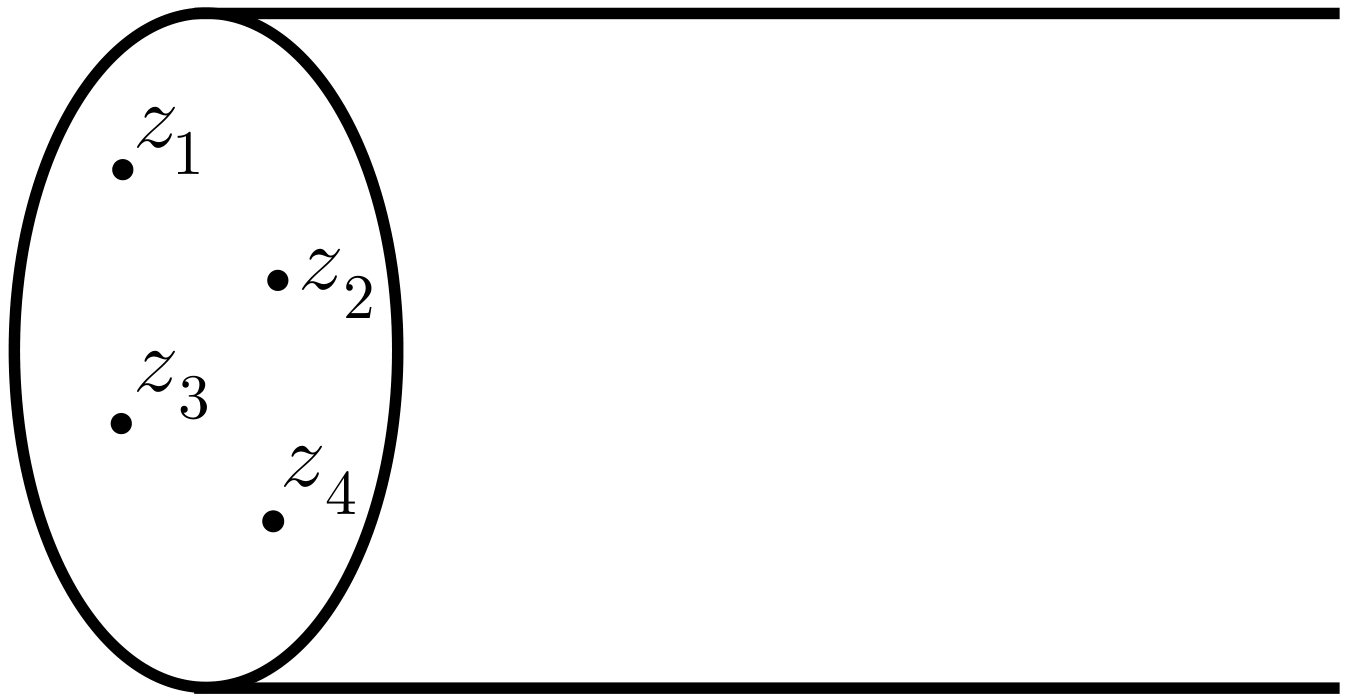
\includegraphics[width=3.5in]{figs/Fig06.png}
 \end{center}
\caption{\small  一个与时间无关的情形在固定时刻的快照。在三流形 $M_3=C\times \R_+$ 中，纽结出现在边界点 $z_1,\dots,z_4$ 处。（原稿第 45 页）}
 \label{again}
\end{figure}
我们从与时间无关的情形开始——四流形 $\MM=\R\times \Mthree$ 上的扭曲 $\N=4$ 超 Yang-Mills 理论，其中 $\Mthree$ 是一个三流形，而我们把 $\R$ 看作时间方向。在我们的应用中，$\Mthree=C\times \R_+$，$C$ 是黎曼面。若存在纽结，我们一开始假设它们与时间无关。在这种情形下（为方便起见，图~\ref{again} 再次描绘了它），我们要找出 BPS 态——量子基态。

第一步近似——已在第~\ref{teqone}~节与第~\ref{analog}~节中分析过——是寻找与时间无关的经典解。从经典解过渡到 BPS 态时，我们将忽略 $\Mthree$ 的非紧性。这意味着我们将忽略非 BPS 激发的连续谱的存在。


 若 BPS 方程只有有限多个经典解（且它们非退化——即围绕这样的解展开时没有零模），则 BPS 态空间的经典近似非常简单。令 $\I$ 为经典解的集合。于是对每个 $I\in \I$，微扰论中存在一个定域在 $I$ 附近的量子基态 $\psi_I$。在微扰论中，$\psi_I$ 构成 BPS 态空间 $\H$ 的一组基。

非微扰地看，在这类一般问题中，瞬子效应可能把这些近似基态中的一些从零能处抬升。然而，我们这里处理的实际上是不会发生这种情况的问题。这是因为在与时间无关的情形下，即便存在纽结，我们的问题也有四个超荷，而一个瞬子（即具有非平凡时间依赖性的经典解）至少破坏其中两个。这导致瞬子背景中出现两个费米零模，这比在近似基态 $\psi_I$ 与 $\psi_J$ 之间为超荷 $Q$ 的矩阵元作贡献所需的零模数多了一个。

\subsubsection{与 Morse 理论的关系}\label{relm}

关于瞬子为何不抬升经典真空简并性，一个更明确的理解来自于本问题与 Morse 理论的关系。\footnote{关于 Morse 理论相关方面相对易懂的介绍，见文献~\cite{hutchings}。}与 Morse 理论相关的超对称量子力学（文献~\cite{Morse}）一般是从 $\R$ 到 $\U$ 的映射的理论，其中 $\U$ 是带有度规张量 $g$ 的黎曼流形，并配有一个我们称为超势的实值函数 $h$。对一般的 $\U$ 与 $h$，该模型有两个超荷，其中一个与外微分共轭：
\begin{equation}\label{zolmo} Q=e^h\d e^{-h}.\end{equation}
经典真空对应于 $h$ 的临界点。若 $h$ 是 Morse 函数——即其临界点都是孤立且非退化的——则在微扰论中，每个临界点 $I$ 对应一个近似量子基态 $\psi_I$。$\psi_I$ 的费米子数 $q_I$ 等于临界点 $I$ 的 Morse 指标（即函数 $h$ 在 $I$ 处二阶导数矩阵的负本征值个数）。由于 $Q$ 使费米子数增加一个单位，只有当
\begin{equation}\label{yre} q_J=q_I+1.\end{equation}
时，才可能由量子修正诱导出非零矩阵元 $\langle \psi_J|Q|\psi_I\rangle$。这类非零矩阵元可以通过在适当意义下计数在远过去始于临界点 $I$、在远未来终于临界点 $J$ 的瞬子解来计算。相应的“瞬子”方程，换言之，映射 $\R\to \U$ 为 $Q$ 不变的条件，就是 Morse 理论的梯度流方程：
\begin{equation}\label{orlox} \frac{\d x^i}{\d t}=-g^{ij}\frac{\partial h}{\partial x^j}.\end{equation}

我们正在研究的 $\R\times \Mthree$ 上的扭曲 $\N=4$ 超 Yang-Mills 理论问题（我们主要取 $\Mthree=C\times\R_+$，但以下论述更为一般）就是这种类型的无穷维问题，\footnote{\label{zort}
更准确地说，我们的问题是这类问题的一个规范不变版本——对应于一个以 $\U$ 为目标、并与把 $\U$ 的一个对称性规范化的规范场耦合的超对称 sigma 模型。在我们的情形中，规范群是从 $\Mthree$ 到有限维群 $G$ 的映射构成的群，而 $\U$ 是 $\Mthree$ 上复值联络的空间。然而，在我们的问题中规范群自由地作用在 $\U$ 上；这由 Nahm 极点边界条件保证。因此，规范不变性不会起主要作用。实际上，就我们的目的而言，我们可以把 $\U$ 换作它对该复规范变换群的商，从而约化为没有规范场的情形。}其中 $\U$ 是 $\Mthree$ 上复值联络的空间。我们把 Chern-Simons 函数
\begin{equation}\label{csfun}\W=\frac{1}{4\pi i }\int_{\Mthree}\,\Tr\,\left(\A\wedge\d \A+\frac{2}{3}
\A\wedge\A\wedge\A\right)\end{equation}
看作复流形 $\U$ 上的全纯函数。全纯性意味着以 $\U$ 为目标、以 $\W$ 为超势的一维 sigma 模型有四个超荷（这实际上依赖于 $\U$ 的度规是 Kähler 度规这一事实，并且在脚注~\ref{zort} 提到的规范不变情形下也成立）。我们实际上希望在与 $\N=4$ 超 Yang-Mills 理论的某种扭曲相联系的框架中研究这个模型，其中某个特定的超荷 $Q$ 被专门标记出来。这个超荷依赖于扭曲参数 $\t$（文献~\cite{KW}），并且是 $Q=e^h\d e^{-h}$ 的无穷维版本，其中 $h$ 是通常的 Morse 函数
\begin{equation}\label{morsefn}h=\mathrm{Re}\,(e^{i\alpha}\W),\end{equation}
并且
\begin{equation}\label{alphaq} \t = \frac{1- \sin \alpha}{\cos{\alpha} }\end{equation}
对于这种类型的 Morse 函数，梯度流方程变为
\begin{equation}\label{lphaq} \frac{\d \bar w^{\bar j}}{\d t}=-g^{\bar j i}\frac{e^{i\alpha}}{2}
\frac{\partial\W}{\partial w^i},\end{equation}
其中 $w^i$ 是 $\U$ 上的局部全纯坐标。


我们的问题与 Morse 理论相联系的一个具体表现是：底层的四维超对称方程 (\ref{bpseqns}) 正是无穷维流形 $\U$ 上 Morse 函数 $h$ 的梯度流方程 (\ref{orlox})。（这是文献~\cite{Analytic,NewLook} 的主要思想之一，其中已把脚注~\ref{zort} 提到的规范不变性考虑在内。）

现在我们可以更明确地解释为什么我们的问题中的非微扰效应不会破坏任何近似量子基态 $\psi_I$ 的超对称性。一般地，对于作为全纯函数实部的 Morse 函数，孤立的临界点都有相同的（中间维数的）Morse 指标，从而有相同的费米子数 $q$。因此条件 (\ref{yre}) 永远不会被满足。

得到同一结果的另一条途径如下。一般地，对于像 $h$ 这样作为全纯函数实部的 Morse 函数，梯度流有一个守恒量，即相应全纯函数的虚部，在我们的情形中为
\begin{equation}\label{conserved}  j = \mathrm{Im}\,(e^{i\alpha}\W). \end{equation}
对一般的 $\alpha$，所有临界点都有不同的 $j$ 值，因此不同的临界点不可能被梯度流方程的解连接起来。于是不存在可能破坏态 $\psi_I$ 超对称性的瞬子。

\subsubsection{时间依赖}\label{time}

正如第~\ref{methods}~节所解释的，我们并不真的想考虑与时间无关的情形；我们想要允许纽结位置的缓慢时间依赖。令 $\ZZ$ 为互不相同的点 $z_1,\dots,z_d\in C$ 构成的空间。BPS 态空间 $\H$ 是 $\ZZ$ 上一个丛 $\hat\H$ 的纤维。这个丛带有自然的平坦联络。这是拓扑场论的一般性质，而 Morse 理论的解释给出了特别好的描述。

在与 Morse 理论相关的超对称量子力学中，由于超荷 $Q=e^h\d e^{-h}$ 与外微分 $\d$ 共轭，与临界点相联系的基态 $\psi_I$ 必然可以用 $\U$ 的上同调、或对偶地用同调来解释。Morse 理论中有一个标准的方式来理解这一点。对临界点 $I$，人们联系一个向下流的链 $\J_I$，它由 $\U$ 中所有可以从 $I$ 出发经梯度流到达的点组成。换言之，考察半直线 $(-\infty,0]$ 上梯度流方程的解，其初始条件为流在 $t=-\infty$ 时从 $I$ 出发。$\J_I$ 参数化了这类流在 $t=0$ 时的取值。
% [Tutor Note: 物理图像] “向下流的链”即从临界点 $I$ 出发沿 $-\nabla h$ 方向流出的轨迹的并集；在 Morse 理论中它同胚于一个开胞腔，其维数等于 $I$ 的不稳定流形维数，即 Morse 指标。于是 $\partial\J_I$ 由从 $I$ 流向更低临界点的流线组成，这正是 Morse 链复形中边缘算符的几何来源。

$h$ 为全纯函数实部的情形具有特殊性质，并且特别简单，所以让我们集中讨论这一情形。我们进一步作简化假设：$h$ 的临界点是孤立且不可约的。$\U$ 必然是非紧的（否则它不能容纳非常值全纯函数）。在这种非常特殊的情形下，$\J_I$ 称为 Lefschetz thimble（Lefschetz 针）。若在定义 $h$ 时所用的角 $\alpha$ 足够一般（以阻止不同临界点之间存在梯度流），则这些针 $\J_I$ 是闭的，但它们不是紧的。因此它们并不代表 $\U$ 的通常同调中的类。然而，由于 $\J_I$ 是相对于 $h$ 的向下梯度流定义的，沿 $\J_I$ 到无穷远有 $h\to -\infty$。因此 $\J_I$ 是某个相对同调群的元素——即 $\U$ 相对于区域 $\U_<$ 的同调 $H(\U,\U_<)$，在该区域中 $h$ 趋于 $-\infty$。（在记号中我们没有标明同调链的维数，因为这个相对同调只在中间维数上非零。这与所有临界点都具有中间维数 Morse 指标这一事实有关。）

超对称基态的空间 $\hat\H$ 可以等同于相对同调 $H(\U,\U_<)$。在这一对应中，与临界点 $I$ 相联系的量子基态 $\psi_I$ 映到 $H(\U,\U_<)$ 的元素 $\J_I$。关于这一点的物理说明（在与 Morse 理论相关的超对称量子力学的语境中），见文献~\cite{FLN} 或文献~\cite{NewLook}。

用相对同调来解释，意味着 $\hat\H$ 具有整结构，从而具有自然的平坦联络。给它一个漂亮的名字：这个平坦联络就是相对同调上的 Gauss-Manin 联络。对一般的 $\alpha$ 与 $z_i$ 值，这个联络是平凡的：$\psi_I$ 是平坦截面，而 $\hat\H$ 上的联络完全由经典临界点及相应针的光滑演化描述。（在搬运针时必须追踪其定向；与 $\J_I$ 相联系的相对同调类的符号依赖于 $\J_I$ 的定向。）

关键之处在于，在参数 $\alpha$ 与 $z_i$ 的空间 $S^1 \times \ZZ$ 中存在余维一的面，在那里针不再是闭的（因而不再定义相对同调的元素），而从临界点到量子态的映射发生不连续的跳跃。若存在从 $I$ 到 $J$ 的梯度流线，就会发生这种情况；此时 $\J_I$ 不是闭的，因为它含有任意接近 $J$ 但不含 $J$ 本身的点。

我们把 $S^1\times \ZZ$ 中使如下必要条件得到满足的轨迹记作 $\ell_I^J$，这些条件是：对从 $I$ 到 $J$ 的流，守恒量 $j$ 在 $I$ 与 $J$ 处相等，而 $h(I)>h(J)$。第一个条件是一个实条件，第二个只是一个不等式。因此 $\ell_I^J$ 的实余维为 1，我们称它为 Stokes 墙。
% [Tutor Note: 易错点] Stokes 墙的余维数为 1 完全来自 $j(I)=j(J)$ 这一个实方程；$h(I)>h(J)$ 只是开条件（决定墙的哪一侧可用），不降低维数。若把 $h(I)>h(J)$ 也当成独立条件，就会误以为余维是 2，从而错过“穿墙”在余维 1 处发生的图像。

穿过 Stokes 墙 $\ell_I^J$ 时，只有针 $\J_I$ 变得不良定义。它按 $\J_J$ 的倍数跳跃：
\begin{equation}\label{stokesS}
\J_I \to \J_I + \frak{m}_{IJ} \J_J,
\end{equation}
其中 $\frak{m}_{IJ}$ 是从 $I$ 到 $J$ 的梯度流线在适当意义下的“数目”。给定一条线对符号贡献 1 或 $-1$，取决于 $j=\mathrm{Im}(e^{i \alpha} \W(w,z))$ 在 $I$ 与 $J$ 处取值之差经过零的方向。关于这类事情的初级说明，见文献~\cite{Analytic} 第 2 节。

态 $\psi_I$ 与针 $\J_I$ 之间的对应意味着 $\psi_I$ 在穿过 Stokes 墙时有相同的跳跃。在 $\psi_I$ 基下，除跨过 Stokes 墙之外联络是平凡的，而在跨越处的传输矩阵是一个三角形的“Stokes 因子”
\begin{equation}\label{sf}
S[\ell_I^J] = 1 + \frak{m}_{IJ} e^J{}_I
\end{equation}
这里 $e^J{}_I$ 是唯一非零元为 $1$、位置在第 $J$ 行第 $I$ 列的矩阵。

特别地，沿 $S^1 \times \ZZ$ 中路径 $\P$ 的平行移动是如下类型因子的路径有序乘积：(a) 在两个 Stokes 墙之间，只有“形式单值性”，它表达经典临界点的置换，并带有追踪针定向的负号；(b) 每穿过一个 Stokes 墙，单值性就获得相应的 Stokes 因子。


人们可以把路径 $\P$ 的传输矩阵的矩阵元 $\frak{n}_I^J[ \P ]$ 形象地看作从临界点 $I$ 到临界点 $J$ 的路径计数：在远离 Stokes 墙处，必须连续地跟随一个临界点；但在穿过一面墙时，允许沿一条从某个临界点到下一个临界点的梯度流轨迹“跳跃”。传输矩阵的矩阵元由这类混合路径的贡献之和给出，每条路径贡献 1 或 $-1$，取决于针的定向沿给定路径如何演化。


顺便说一句，沿路径 $\P$ 平行移动的单值性只依赖于 $\P$ 的同伦类，这一事实蕴含控制跳跃的数 $\frak{m}_{IJ}$ 满足穿墙公式。更一般地，整个图像可以用基于 $\W$ 的 LG 模型中的 BPS 态来解释，但本文不再追究这一解释。

让我们汇集矩阵元 $\frak{n}_I^J[ \P ]$ 的一些性质：
\begin{itemize}
 \item $\frak{n}_I^J[ \P ]$ 只依赖于 $\P$ 的同伦类；
  \item 路径的复合对应矩阵乘法：
  $\frak{n}_I^K[ \P_1 \circ \P_2 ]= \sum_J\frak{n}_I^J[ \P_1 ]\frak{n}_J^K[ \P_2 ]$；
  \item 对从 $z$ 到 $z + \delta z$ 的无穷小路径 $\delta \P$，几乎总有 $\frak{n}_I^J[ \delta \P ] = \delta_I^J$——只有穿过 Stokes 墙时这一点才不成立；
  \item 穿过 Stokes 墙时，$\frak{n}_I^J[ \delta \P ] - \delta_I^J = \frak{m}_{IJ}$，其中 $\frak{m}_{IJ}$ 由流线计数算出。
\end{itemize}

\subsubsection{对偶基}\label{dual}


若 $\Gamma$ 是相对同调 $H(\U,\U_<)$ 中的任一同调链，则由针构成该相对同调的一组基，$\Gamma$ 在相对同调中等价于针的线性组合，
 \begin{equation}\label{holm} \Gamma=\sum_I\frak c^I \J_I.\end{equation}
系数 $\frak c^I$ 如何确定？若我们在某种意义上有一个与 $\J_I$ 对偶的基 $\K^I$，其配对为
\begin{equation}\label{oggo} \langle \K^J,\J_I\rangle=\delta^J{}_I,\end{equation}
那么我们就会把 (\ref{holm}) 中的系数确定为
\begin{equation}\label{ggo} \frak c^I=\langle \K^I,\Gamma\rangle.\end{equation}

相对同调 $H(\U,\U_<)$ 的 Poincar\'e 对偶是相反方向的相对同调 $H(\U,\U_>)$，即 $\U$ 相对于 $h\to+\infty$ 的区域 $\U_>$ 的相对同调。$H(\U,\U_>)$ 的一组自然基由与临界点相联系的向上流的针 $\K^I$ 给出。对每个临界点 $I$，$\K^I$ 定义为半直线 $[0,\infty)$ 上梯度流方程的解在 $t=0$ 处的边界值，这些解在 $t\to+\infty$ 时趋向点 $I$。由于 $h$ 沿梯度流线递减，它沿这样的流所取的最小值就是其在 $t=\infty$ 处的值，即其在临界点 $I$ 处的值。因此 $h$ 沿 $\K^I$ 有下界，但可能没有上界，而 $\K^I$ 取值于 $H(\U,\U_>)$。至于配对 (\ref{oggo})，由 $\K$ 与 $\J$ 的定义，$\langle\K^J,\J_I\rangle$ 计数整条实直线 $(-\infty,\infty)$ 上在 $t=-\infty$ 时始于 $J$、在 $t=+\infty$ 时终于 $I$ 的流。对 $J\not=I$，不存在这样的流（对针有良好定义的一般 $\alpha$ 而言）。对 $J=I$，由于 $h$ 沿非常值流严格递减，唯一的流是始终停留在 $J$ 的常值流。对 $\J$ 与 $\K$ 的某种自然相对定向，常值流对配对的贡献为 $+1$。
% [Tutor Note: 验证计算] 配对 $\langle\K^J,\J_I\rangle$ 在几何上就是相对同调与对偶相对同调之间的交截数：$\K^J$ 是从 $J$ 向上流的针，$\J_I$ 是从 $I$ 向下流的针，二者的交点只能是沿整条实轴、两端分别停在 $J$ 与 $I$ 的梯度流线。$J\ne I$ 时这种流不存在，故配对为零；$J=I$ 时只有常值流，取适当相对定向后贡献 $+1$，于是正好给出 $\delta^J{}_I$。
   % §3-§4 过渡
\subsubsection{非单值超势与 $q$-分次}\label{nonsingle}

在迄今所给出的框架中，表示辫群在 $\H$ 上作用的矩阵其元素取整数值，因为相对同调具有整结构。现在我们要考虑 $\W$ 非单值的情形。更准确地说，我们将考虑像 Chern-Simons 泛函 $\W$ 那样的全纯函数：其实部单值，但虚部只模 $2 \pi \Z$ 有定义。只要把 $\U$ 换成使 $\W$ 单值的最小覆盖 $\hat \U$，就可以化归到我们迄今所用的框架。

转到 $\hat\U$ 的代价是临界点的数目变成无穷多，因为 $\U$ 中每个临界点在 $\hat \U$ 中都有无穷多个原像。$\hat \U$ 中的一个临界点 $\hat I$ 等同于 $\U$ 中的一个临界点 $I$ 连同在 $I$ 处对 $\W$ 的一条分支的选取。局部地，我们可以任取临界点 $I$ 的一个原像 $\hat I_0$，并把 $\W$ 的值比 $\hat I_0$ 处的值平移 $-2 \pi i n$ 的那个临界点记作 $\hat I_n$。

Stokes 因子与传输矩阵现在是无穷维矩阵，但其矩阵元可以用我们已描述的技术计算，且取整数值。由于这些计算只依赖于 $\W$ 的梯度，这些矩阵与覆叠变换 $\hat I_n \to \hat I_{n+1}$ 对易。引入一个取值于 $\C^*$ 的变量 $q$ 是方便的。于是，若我们简单地把 $q^n\psi_I$ 写成 $\psi_{\hat I_n}$ 的符号缩写，就可以把元素为整数的无穷维矩阵替换为元素为整系数 $q$ 的 Laurent 多项式的有限维矩阵。我们把这样的矩阵记作 $S[\ell_I^J;q]$。为了追踪在 $\ZZ$ 中移动时 $\W$ 的提升，编码临界点置换的形式单值矩阵以及与梯度流相联系的 Stokes 矩阵都取值于 $q$ 的幂，以追踪沿路径 $\W$ 的变化。传输矩阵的矩阵元现在通过对混合路径（远离 Stokes 墙处的连续演化与穿过 Stokes 墙的梯度流）求和得到，权重为 $\pm q^n$，其中 $-2\pi i n$ 是超势沿路径的变化，而符号一如既往地涉及针的定向。

对这一切还有一种等价的描述。由于 $\U$ 容许非单值超势 $\W$，其第一 Betti 数为正，人们可以在超对称量子力学中引入一个“theta 角” $\theta$，对 $\W$ 跳跃 $-2\pi i n$ 的路径加权 $e^{in\theta}$。其效果是把 $\U$ 的相对同调换成一个扭曲的相对同调，取值于单值性为 $q=e^{i\theta}$ 的平坦线丛。然后我们考虑由这个平坦丛扭曲的同调的 Gauss-Manin 联络。该联络的和乐矩阵其元素为整系数 $q$ 的 Laurent 多项式，并且可以按刚才描述的方式计算。
% [Tutor Note: 易错点] 本节的 $q$ 是形式变量（用于把无穷维整矩阵压缩为有限维 Laurent 多项式），而第~\ref{clco}~节之后（如 (\ref{torg})、(\ref{zorg})）的 $q$ 是取数值的 Jones 参数 $q=\exp(2\pi i/(\k^\vee+2))=\exp(-2\pi i/b^2)$。两者在本文中同名，但一为形式、一为数值，读到 $q^n$、Laurent 多项式时不要误代入数值。




\subsection{四维解计数的经典描述}\label{clco}

现在让我们考虑真正感兴趣的问题——$\R\times C\times \R_+$ 上超对称方程 (\ref{bpseqns}) 的依赖时间的解。解之所以依赖时间，是因为边界条件依赖时间——我们允许 $\Mthree=C\times \R_+$ 边界上的奇异磁单极子的位置 $z_i$ 随时间变化。虽然我们通常假定磁单极子位置作绝热演化，但四维解的计数是拓扑的，绝热假定并非必需。



在最简单的设定中，边界处的奇异磁单极子股在时间中编织，超势全纯地依赖于某些参数（即各股在 $C$ 中的位置），而这些参数随时间演化。概略地说，方程取“受迫梯度流”的形式
\begin{equation} \label{flow}
\frac{\d \bar w_{\bar i}}{\d t} = -e^{i \alpha} g^{\bar i j}  \frac{\partial \W(w,z(t))}{\partial w_j}
\end{equation}

我们假定这些奇异磁单极子在 $t=-\infty$ 附近从位置 $\vec z_i=(z_{1},\dots,z_{k})$ 出发，并在 $t=+\infty$ 附近终止于位置 $\vec z_f=(z'_{1},\dots,z'_{k})$。事实上，我们可以假定奇异磁单极子的位置 $z_i(t)$ 除在某个有界区间 $-T<t<T$（$T$ 为某值）内之外都是常数，而在这个区间内它们沿其参数空间 $\ZZ$ 中的一条路径 $\P$ 运动。在这种情形下，我们可以寻找受迫梯度流方程的解：它们在 $\W(w,\vec z_i)$ 的某个指定临界点 $I$ 出发，终止于 $\W(w,\vec z_f)$ 的某个指定临界点 $J$。这类解的“数目”（每个解按费米子行列式的符号加权）是一个拓扑不变量——在路径 $\P$ 或 $\U$ 上度规的形变下不变。我们把这个不变量记作 $\frak N^J_I$。（由于一个马上就会明白的原因，我们实际上只想在 $\vec z_i$ 与 $\vec z_f$ 不在 Stokes 墙上时定义 $\frak N^J_I$。）

在第~\ref{time}~节中，我们已经为这种情形联系了一个整数不变量 $\frak n^J_I[\P]$。$\frak n^J_I[\P]$ 是沿从 $\vec z_i$ 到 $\vec z_f$ 的路径 $\P$ 作平行移动的 Gauss-Manin 联络的矩阵元。可以把 $\frak n^J_I[\P]$ 看作这样的展开系数：把相对同调 $H(\U,\U_<)_{\vec z_i}$ 中的一个针 $\J_I$ 沿路径 $\P$ 用 Gauss-Manin 联络搬运，然后再用构成 $H(\U,\U_<)_{\vec z_f}$ 的一组基的针 $\J'_J$ 来表示：
\be\label{zelx}\J_I=\sum_J\frak n^J_I \J'_J.\ee
我们断言，事实上
\be\label{elx}\frak N^J_I=\frak n^J_I.\ee
这一关系的重要性在于：$\frak N^J_I$ 才是我们想要的东西，即依赖时间的解的计数；而 $\frak n^J_I$ 更容易计算，因为它只需研究与时间无关的问题。
% [Tutor Note: 物理图像] (\ref{elx}) 是本节的核心：左边是“真正”的四维（依赖时间）解数，右边是纯三维（与时间无关）的 Gauss-Manin 搬运系数；二者相等意味着时间依赖只把针连续地搬运，不会额外产生或消灭解。实现这一等价的正是“强迫梯度流把 $\J_I$ 连续形变为 $\tilde\J_I$、而相对同调类是离散的”这一事实。



 
对 (\ref{elx}) 的一个解释如下。按定义，$\J_I[\vec z_i] $ 是 $\U$ 中可由如下流
\begin{equation}
\frac{\d \bar w_{\bar i}}{\d t} = -e^{i \alpha} g^{\bar i j}  \frac{\partial \W(w,z_i)}{\partial w_j}
\end{equation}
到达的点的集合，这些流在过去渐近于 $I$。这里 $z_i$ 被看作常数。现在考虑半无穷区间 $(-\infty,t_0]$ 上受迫梯度流的方程 (\ref{flow})。对 $t_0\leq -T$，该方程的解在 $t_0$ 处的取值参数化了 $\J_I[\vec z_i]$；但对 $t_0>-T$，它们参数化了这个空间的一个依赖于 $t_0$ 的连续形变，我们将它记作 $\tilde \J_I[\vec z_i;t_0]$。

我们在第~\ref{dual}~节中看到，对 $H_m(\U ,\U_<)_{\vec z_f}$ 中任一给定的链 $\Gamma$，展开式
\begin{equation}
\Gamma =\sum_J\frak{c}^J \J_J[\vec z_f]
\end{equation}
中的系数 $\frak{c}^J $ 按指标的意义计数了如下流的数目
\begin{equation}
\frac{d \bar w_{\bar i}}{dt} = -e^{i \alpha} g^{\bar i j}  \frac{\partial \W(w,z_i)}{\partial w_j}
\end{equation}
这些流从 $\Gamma$ 出发，在未来渐近于临界点 $J$。

因此，在编织发生之后的某个给定时刻 $t_0$，从 $\tilde \J_I[\vec z_i;t_0]$ 流向未来临界点 $J$ 的四维解的数目，就是展开式
\begin{equation} \label{ntop}
\tilde \J_I[\vec z_i;t_0] =\sum_J\tilde {\frak N}_I^J\J_J[z_f].
\end{equation}
中的系数 $\tilde{\frak N}^J_I$。但由于 $\tilde\J_I[\vec z_i;t_0]$ 参数化了区间 $(-\infty,t_0]$ 上始于 $I$ 的流，从 $\tilde\J_I[\vec z_i;t_0]$ 到 $J$ 在区间 $[t_0,\infty)$ 上的流，等价于定义在整条实直线上的从 $I$ 到 $J$ 的流。所以 $\tilde{\frak N}^J_I$ 与所要的不变量 $\frak N^J_I$ 相同：
\begin{equation} \label{nzop}
\tilde \J_I[\vec z_i;t_0] =\sum_J\frak N^J_I  \J_J[z_f]
\end{equation}
相对同调定义在 $\Z$ 上，而像 $\tilde\J_I$ 这样的整相对同调类没有连续形变。因此很清楚：只要由流方程 (\ref{flow}) 诱导的、从 $\J_I[\vec z_i]$ 到 $\tilde \J_I[\vec z;t_0]$ 的连续形变在任一给定时刻都落在 $H_m(\U ,\U_<)_{\vec z(t)}$ 中，它就与沿 $\P$ 由 Gauss-Manin 联络给出的自然搬运一致。在这种情形下，(\ref{nzop}) 等价于所要的结果 $\frak{N}^J_I = \frak{n}^J_I$。

为证明对任意 $t_0$ 都有 $\tilde\J_I[\vec z;t_0]$ 落在 $H_m(\U,\U_<)_{\vec z(t_0)}$ 中，我们应当证明 $\mathrm{Re}\,\W(w,\vec z(t_0))$ 沿 $\tilde \J_I[t_0]$ 到无穷远趋于 $-\infty$。确实，若半无穷区间 $(-\infty,t_0]$ 上的一列受迫梯度流趋于无穷远，它一定是通过 $t\to t_0$ 时发散而趋于无穷远的；在这种情形下，$\mathrm{Re}(\W(w,z(t_0))$（其梯度驱动 $t\to t_0$ 时的流）必须趋于 $-\infty$。

对 (\ref{elx}) 的另一种论证如下。假定 $\vec z_f=\vec z_i$，且 $\P$ 是它们之间的平凡路径。那么 $\frak N^J_I=\frak n^J_I=\delta^J_I$。当我们变动 $\vec z_f$ 时，$\frak N^J_I$ 与 $\frak n^J_I$ 都只可能在穿过 Stokes 墙时跳跃；它们的跳跃方式完全相同，因此始终保持相等。我们已经描述了 $\frak n^J_I$ 的跳跃。$\frak N^J_I$ 的跳跃之所以发生，是因为在穿过 Stokes 墙时，一个依赖时间的解可能消失到无穷远，具体如下。假定对某个 Stokes 墙上的 $\vec z_f$，$\frak n^J_I$ 发生跳跃，其来源是从 $\W(w,\vec z_f)$ 的某个临界点 $J'$ 到 $J$ 的一条普通梯度流。这样的流产生跳跃
\be\label{jumpo} \frak n^J_I\to \frak n^J_I\pm \frak n^{J'}_I,\ee
其中符号取决于穿过 Stokes 墙的方向。为看到 $\frak N^J_I$ 中相应的跳跃，人们寻找从 $I$ 到 $J$ 的受迫梯度轨迹，它由一条从 $I$ 到 $J'$ 的受迫梯度轨迹、随后在某个非常遥远的未来时刻接上同一条引起 $\frak n^J_I$ 跳跃的从 $J'$ 到 $J$ 的普通梯度轨迹所组成。若 $\vec z_f$ 靠近 Stokes 墙且位于其正确的一侧，这种两步受迫轨迹就存在；当 $\vec z_f$ 穿过 Stokes 墙时，流发生第二步的时刻发散。这导致两步解消失，并使 $\frak N^J_I$ 产生一个恰好与 $\frak n^J_I$ 的跳跃相配的跳跃。




\section{从针的编织到自由场积分}\label{fthimconformal}
\begin{keytakeaways}
\begin{itemize}\setlength{\itemsep}{2pt}
  \item \textbf{物理图像}：把相对同调的链看作积分链，BPS 态随参数的演化就等价于这些积分随参数的演化；针上的积分在 $\varepsilon\to0$ 的半经典极限下由临界点主导，故可用最速下降/Picard-Lefschetz 方法来计算。
  \item \textbf{数学工具}：相对同调上的 Gauss-Manin 联络与 Stokes 理论、针上的渐近展开、复结构形变（Beltrami 微分）、Chern-Simons 路径积分与共形块。
  \item \textbf{主要结论}：$\Mthree=C\times\R_+$ 上针的积分等同于带 Nahm 极点边界条件的 $\N=4$ 理论在 $M_3\times\tilde\R_+$ 上的配分函数；两个 Chern-Simons 描述由 $S$ 对偶相联系，其能级满足 $\k+2=1/(\k^\vee+2)$。
  \item \textbf{共形块}：oper 边界条件（$\A_z$ 上三角且右上元为 1、$\A_{\bar z}$ 下三角）诱导出 Virasoro 共形块，且 Jones 参数与 $b$ 满足 $q=\exp(-2\pi i/b^2)$。
\end{itemize}
\end{keytakeaways}

根据第~\ref{fourd}~节的论证，为理解与 Jones 多项式相联系的辫群表示，我们应当计算三流形 $\Mthree=C\times \R_+$ 上联络的无穷维空间 $\U$ 的中间维相对同调上的一个自然单值性作用。这听起来可能抽象得令人绝望。现在我们将说明，它可以转化为某种具体且可计算的东西。


\subsection{从针到积分}\label{fromth}



描述 $\H$ 中态的演化（包括 $q$-分次）的一种方便方式，是把同调链看作积分链。不考察同调链的演化，等价地可以考察积分的演化。当然，我们需要一个可以在针 $\J_I$ 上积分的被积函数，而针不是紧的。满足这一要求的函数是 $e^{\W/\varepsilon}$，其中 $\varepsilon$ 选取在适当的半平面内。由于
\begin{equation}
h = \mathrm{Re} \left( e^{i \alpha} \W \right)
\end{equation}
沿针趋于负无穷，我们所要的条件是 $\mathrm{Re} \left( e^{i \alpha} \varepsilon\right)>0$。这将保证积分
\begin{equation}\label{thelko}
\I_\Gamma = \oint_\Gamma e^{\W(w)/\varepsilon} \d \Omega
\end{equation}
收敛，其中 $\d\Omega$ 是 $\U$ 上的全纯体积形式（下文将保持固定），而积分链 $\Gamma$ 是一个针，或更一般地是相对同调 $H(\U,\U_<)$ 中的任一链。

针是特别好的积分链，因为针上积分的 $\varepsilon\to 0$ 极限非常简单。在由从临界点 $I$ 出发的梯度流定义的针 $\J_I$ 上，函数 $h$ 有唯一的最大值，即该临界点。因此当 $\varepsilon\to 0$ 时，针上的积分为
\begin{equation}\label{thelk}
\I_I:= \oint_{\J_I} e^{ \W(w)/\varepsilon}\, \d \Omega\sim \exp(\W_I/\varepsilon)\left(\varepsilon^{-\mathrm{dim}\,\J_I/2}c_0+\dots\right),
\end{equation}
其中 $\W_I$ 是 $\W$ 在临界点 $I$ 处的值。
% [Tutor Note: 验证计算] (\ref{thelk}) 的幂次 $\varepsilon^{-\mathrm{dim}\,\J_I/2}$ 来自针上的高斯型积分：$\J_I$ 的实维数等于 $\U$ 的复维数（也就是这里所说的“中间维”），沿其做 $\mathrm{dim}\,\J_I$ 个实方向的鞍点积分，每个实方向贡献 $\varepsilon^{-1/2}$，合起来便是 $\varepsilon^{-\mathrm{dim}\,\J_I/2}$。注意不要把 $\mathrm{dim}\,\J_I$ 与某个复维数混用，否则幂次会差因子 $2$。

这个公式在整个半平面 $\mathrm{Re} \left( e^{i \alpha} \varepsilon\right)>0$ 内成立；但实际上只要 $\alpha$ 不在 Stokes 墙上，这个渐近式在复平面内稍大一些的扇区内也成立。\footnote{\label{breakdown}为使所述的渐近式失效，第一步是穿过一面 Stokes 墙，于是我们出发时的针演化为至少含两项的针的线性组合。起初，渐近式 (\ref{thelk}) 仍然成立，因为 Stokes 墙上新出现的那些额外的针起初只贡献指数小的量。若把 $\alpha$ 继续变动，其中一个额外针最终可能占主导。整个过程总是涉及把 $\alpha$ 从其初值变动一个严格大于 $\pi/2$ 的角度。为说明这一点，只需比较 $\W$ 在两个临界点处的值；这些值在 Stokes 墙上虚部相等，而在两个临界点交换主导地位时实部相等。}这一性质唯一地刻画了所有可能的 $I_\Gamma$ 中积分基 $\I_I$：若取几个 $\I_I$ 的线性组合，则渐近式会在扩展半平面内的某条射线上失效，在彼处两个临界点交换主导地位。这一刻画在 Stokes 理论中为人熟知，也正是“Stokes 墙”这一术语的由来。

当 $\W$ 的参数变动时，同调 $H(\U,\U_<)$ 连续地变动。若把积分链 $\Gamma$ 连续地变动，积分将全纯地依赖于 $\W$ 的参数。链 $\Gamma$ 的单值性与积分 $\I_\Gamma$ 的单值性相同。

\subsection{两个 Chern-Simons 理论}
在我们当前的语境中，针的积分 (\ref{thelko}) 是三流形 $\Mthree = C \times \R_+$ 上的 Chern-Simons 路径积分，只不过是在一个不寻常的积分链上。这样的积分可以用 $\Mthree \times \tilde \R_+$ 上的 $\N=4$ 规范场论具体地表达出来。（仅在本节中，我们把 $x^1$ 方向写作 $\tilde \R$ 或 $\tilde\R_+$，以区别于 $y$ 方向 $\R_+$。）这一陈述是文献~\cite{Analytic, NewLook} 的主要结论之一。在我们的情形中，由于 $\Mthree = C \times \R_+$，四维流形是 $M_4 = C \times \R_+ \times \tilde \R_+$。

这是本文中出现的第二个 Chern-Simons 理论，至少是隐含地出现。我们的全部分析都关乎 Jones 多项式的计算，所用的规范场论设定 $S$ 对偶于一个通过在 $W = C \times \tilde \R$ 上的 Chern-Simons 理论计算 Jones 多项式的设定。在那个“原始的” Chern-Simons 理论中，纽结是一条 Wilson 圈，规范群是 $G^\vee$，耦合参数是 $\k^\vee$。Jones 多项式是如下量的 Laurent 多项式：
\begin{equation}\label{torg} q=\exp(2\pi i/(\k^\vee+2)),\end{equation}
其中 $2$ 是 $SU(2)$ 的对偶 Coxeter 数。

正如文献~\cite{fiveknots} 所解释的，若把 $\k^\vee$ 与 $\N=4$ 理论的扭曲参数 $\Psi^\vee$ 通过
\begin{equation} \label{psikvee} \Psi^\vee=\pm (\k^\vee+2). \end{equation}
相联系，则三流形 $W$ 上的 Chern-Simons 理论可以通过 $W\times \R_+$ 上的拓扑扭曲 $\N=4$ 超 Yang-Mills 理论来计算。在这一描述中，人们在 $\R_+$ 的原点处使用 D3-NS5 边界条件。符号 $\pm$ 取决于 $M_4$ 与 $W$ 之间定向的相对选取。

人们还可以应用 $S$ 对偶，把规范群从 $G^\vee=SU(2)$ 变为 $G=SO(3)$，并把 D3-NS5 边界条件变成 D3-D5 边界条件；如文献~\cite{gw} 所解释的，这个边界条件涉及 Nahm 极点。在这个新的描述中（它正是本文的出发点），扭曲参数为 $\Psi=-1/\Psi^\vee$。由于这个对偶描述很困难，我们尝试按第~\ref{methods}~节首先说明的办法，通过沿一个方向“拉伸” $W$ 来简化它。于是我们用 $\tilde \R\times C$ 来近似 $W$，并寻找 $W\times \R_+$ 上从 $M_3=C\times \R_+$ “拉回”的 BPS 方程的解。若把这个对偶描述表述为以 $\R$ 为时间方向、以 $M_3=C\times \tilde \R_+$ 上的规范场为场变量的超对称量子力学，则超势是 $\Psi$（而非 $\Psi^\vee$）乘以 Chern-Simons 泛函。

然后我们把 $M_3$ 上解的编织与 $M_3$ 上 Chern-Simons 理论的针的编织联系起来，后者我们用 $M_3\times \tilde \R_+$ 上的 $\N=4$ 理论来表达。在这一描述中，我们在 $\tilde \R_+$ 的原点处施加 D3-NS5 边界条件（并在 $\R_+$ 的原点处施加 D3-D5 边界条件）。这一 Chern-Simons 描述的能级 $\k$ 与 $\N=4$ 理论的扭曲参数通过
\begin{equation} \label{psik} \Psi=\mp (\k+2). \end{equation}
相联系。这两个 Chern-Simons 描述由 S 对偶以及 $\R_+$ 与 $\tilde \R_+$ 的角色互换相联系。(\ref{psikvee}) 与 (\ref{psik}) 中符号相反，是因为交换 $\R_+$ 与 $\tilde \R_+$ 会反转 $M_4$ 的定向。
% [Tutor Note: 易错点] 两个符号 $\pm$ 与 $\mp$ 必须配套使用：$S$ 对偶同时把 $\Psi\to-1/\Psi^\vee$ 并交换 $\R_+\leftrightarrow\tilde\R_+$，后者反转 $M_4$ 定向，才导致 (\ref{psik}) 相对 (\ref{psikvee}) 取相反的符号。若忘记定向反转，会得到 $\Psi=+\ (\k+2)$，进而把 (\ref{sdualk}) 的倒数关系写成非倒数关系。

结合 $\Psi=-1/\Psi^\vee$ 与 $\Psi^\vee
=\k^\vee+2$，我们发现：与传统方式下联系 Jones 多项式的 Chern-Simons 描述中的能级 $\k^\vee$，和把 Jones 多项式与 Nahm 极点及 oper 相联系的 Chern-Simons 描述中的能级 $\k$，二者之间的关系是\begin{equation}\label{sdualk} \k+2=1/(\k^\vee+2).\end{equation}
% [Tutor Note: 物理图像] (\ref{sdualk}) 并不是简单的 $\k\leftrightarrow\k^\vee$：注意移位后的能级 $\k+2$ 才参与倒数关系，且两个理论互为强弱耦合（$\k^\vee\to\infty$ 时 $\k\to-2$）。$SU(2)$ 的对偶 Coxeter 数为 $2$，正是 (\ref{torg}) 中出现 $+2$ 的来源；这个 $2$ 在一般群 $G$ 时应换成对偶 Coxeter 数。

这个四维设定——$\N=4$ 理论处在带一个“角”的流形 $M_4 = C \times \R_+ \times \tilde \R_+$ 上——相当有趣，我们相信它值得进一步探讨。本文不再深入。

\subsection{从 Chern-Simons 到共形块}

对本文而言，比 $\Mthree=C \times \R_+$ 上 Chern-Simons 理论与四维的联系更有用的，是它与 $C$ 上共形块的联系。这一陈述最熟悉的版本（文献~\cite{WittenJones}）是：固定 $\A_{\bar z}$ 而让 $\A_z$ 变化的路径积分给出一个 WZW 共形块（即二维流代数中的共形块，其对称群 $G$ 与 Chern-Simons 理论的规范群相同）。对固定的 $\A_{\bar z}$ 作局部变动，就在共形块中插入一个全纯流 $J(z)$：
\begin{equation}
\delta \log \cZ = \int \mathrm{Tr} \langle J_z \rangle \delta A_{\bar z}
\end{equation}

这一陈述有一个类比（文献~\cite{HVerlinde}），在 $SU(2)$ 或 $SO(3)$ 规范场论的情形给出 Virasoro 共形块，而在更高秩规范群的情形给出更一般的 $W$-代数共形块（文献~\cite{Bilal,DeBoer}）。这个类比涉及一种不同的边界条件：以在边界上破坏一部分规范对称为代价，固定 $\A_z$ 的一部分和 $A_{\bar z}$ 的一部分。对规范群 $SU(2)$，导致 Virasoro 共形块的边界条件可简单地表述为：
\begin{align}\label{bcon}
\A_z = \begin{pmatrix} * & 1 \cr * & *\end{pmatrix} \qquad \A_{\bar z} = \begin{pmatrix} \times & 0 \cr * & \times\end{pmatrix}
\end{align}
这里我们把可以自由变动的元素记作 $*$，把固定的元素记作 $\times$。

刚才描述的联络就是一个 oper！（由于 $\A_{\bar z}$ 是下三角形的，带有这个联络的丛有一个全纯子丛 $L$，其截面形如 $\begin{pmatrix}0\cr *\end{pmatrix}$；又因为 $\A_z$ 的右上矩阵元处处不为零，这个子丛处处不被 $\D_z=\partial_z+[\A_z,\,\cdot\,]$ 保持。）所以复边界条件 (\ref{bcon}) 正是第~\ref{analog}~节所研究的 Nahm 极点边界条件所诱导的那个。为说明与 Virasoro 共形块的关系，我们指出：Nahm 极点边界条件依赖于 $C$ 上复结构的一个选取。一旦选定复结构并取局部复坐标 $z$，附近的复结构就可以用 Beltrami 微分 $\mu_{\bar z}^z$ 描述。其关系是：在新的复结构下，复联络空间上的全纯场不是 $\A_{\bar z}$，而是 $\A_{\bar z}-\mu_{\bar z}^z\,\A_z$。作这样的形变，等价于把 (\ref{bcon}) 中 $\A_{\bar z}$ 边界条件里的“$0$”换成 $\mu_{\bar z}^z$（于是现在 $\A_{\bar z}-\mu_{\bar z}^z\A_z$ 是下三角形的）。因此，与复结构改变相联系的边界条件的局部变动会插入一个全纯应力张量
\begin{equation}
\delta \log \cZ = \int \langle T_{zz} \rangle \delta \mu_{\bar z}^z,
\end{equation}
而这导致带有 oper 边界条件的 Chern-Simons 理论与 Virasoro 共形块之间的关系。
% [Tutor Note: 物理图像] 这段把“oper 边界条件”与“复结构形变”联系起来：$\A_z$ 的右上元固定为 1 使得子丛 $L$（截面 $(0,*)$）不被 $\D_z$ 保持（oper 的“不可积”条件），而 $\A_{\bar z}$ 的下三角形式让 $L$ 全纯；Beltrami 微分 $\mu_{\bar z}^z$ 描述复结构的形变，其系数正是应力张量 $T_{zz}$ 的源，于是对边界条件求变分就得到 Virasoro Ward 恒等式的插入。

在半经典极限下，算符 $T_{zz}$ 化为 oper 的经典应力张量 $\bt(z)[\A]$。更准确地说，文献~\cite{HVerlinde} 的参数对应关系是：若定义
\begin{equation}\label{bpar}-b^{-2} =\k+2,\end{equation}
其中 $\k$ 是 Chern-Simons 能级，则应力张量的中心荷为 $c=1+6(b+b^{-1})^2$，且在半经典极限下 $b^2 T(z) \to \bt(z)[\A]$。

若把 (\ref{bpar}) 与 (\ref{sdualk})、(\ref{torg}) 结合起来，我们就得到通常用于描述 Jones 多项式的变量 $q$ 与用于描述 Virasoro 共形块的参数 $b$ 之间的关系：
\begin{equation}\label{zorg}q=\exp(-2\pi i/b^2).\end{equation}

这里我们假定了 $G$ 是 $SU(2)$ 或 $SO(3)$。对一般的规范群 $G$，Nahm 极点与 $W$-代数都由 $G$ 的李代数 $\frak{g}$ 中的一个 $\frak{su}(2)$ 嵌入来标记。检查可以确认，用于定义一般 $W$-代数共形块的边界条件正是由相应的 Nahm 极点所诱导的。
   % §4  四维解与平行移动
\subsubsection{Liouville 理论的类比}\label{analiouville}

尽管本文并不需要这一事实，我们仍应指出：Virasoro 共形块与 Chern-Simons 理论之间的关系，可以简单地推广为 Liouville 理论与 Chern-Simons 理论之间的关系。为在黎曼面 $C$ 上研究 Liouville 理论，人们考虑 $C\times I$ 上的 Chern-Simons 理论，其中 $I$ 是单位区间。在 $I$ 的一端施加 Nahm 极点边界条件，在另一端则施加一个把 $z$ 与 $\bar z$ 互换的 Nahm 极点边界条件变体。Liouville 配分函数与关联函数由全纯和反全纯 Virasoro 共形块组合而成，而这些共形块自然地来自带有上述边界条件的 $C\times I$ 上的 Chern-Simons 理论。（对于紧致对称群的情形，人们已经知道 $C\times I$ 上的 Chern-Simons 理论能够重现 $C$ 上的 WZW 模型。）把我们眼下即将给出的论证稍加推广即可看出：插入在点 $p\in C$ 处的 Liouville 理论的轻退化场与一般初级场，对应于 $p\times I$ 上的 Wilson 算符或单值性缺陷。

在经典极限下，Chern-Simons 理论与 Liouville 理论之间的对应意味着以下内容。带有上述边界条件的 $C\times I$ 上 Chern-Simons 理论的经典解，是 $C$ 上的一个平坦丛，其全纯结构与反全纯结构都满足 oper 条件。确实，Liouville 理论的经典解对应于 $C$ 上一个常负曲率的度规。若 $\omega$ 与 $e$ 分别是该度规的标架（vierbein）与自旋联络，那么我们就能定义相应的 $SL(2,\R)$ 平坦联络 $\A=\omega {\ct}_3+
e_{ z} \ct_++e_{\bar z}\ct_-$。取 $\ct_i$ 的标准表示，则 $\A_z$ 是上三角的，其右上角矩阵元处处非零；而 $\A_{\bar z}$ 是下三角的，其左下角矩阵元处处非零。因此，由该平坦联络定义的全纯结构与反全纯结构都满足 oper 条件，正如在 Chern-Simons 描述中所预期的那样。（反全纯 oper 结构的定义，是把“上三角”矩阵与“下三角”矩阵的角色互换。）于是，这就给出了两个理论在经典层面的映射。



\subsection{Wilson 线算符}\label{wilson}

为进一步理解从带 oper 边界条件的三维 Chern-Simons 理论到二维 Virasoro 共形块的映射，我们将探讨 Wilson 线算符在这一对应中的解释。首先回顾一下：若采用把 Chern-Simons 理论与流代数联系起来的标准边界条件，情形会如何。在此情形下，终止于三维流形 $M_3$ 边界上的 Wilson 线算符，代表在 WZW 共形块中于该边界点处插入一个共形初级场。若该 Wilson 线算符在 $G$ 的有限维表示 $R$ 中变换，则相应的共形初级场也在同一表示中变换。这与下述事实一致：终止于边界上的 Wilson 线算符不是规范不变的，而是在表示 $R$ 中变换，正如 WZW 模型中相应的初级场一样。

终止于施加 Nahm 极点边界条件的边界上的 Wilson 线算符，其类似的解释又是什么？Nahm 极点破坏了边界处的规范对称性，因此我们必须选取 Wilson 线算符的某个分量。正如我们在第~\ref{flatpole}~节中所讨论的，一般的矢量平行移动到边界时会发散。给定一个终止于 $y=0$ 的 Wilson 线算符，最容易定义的规范不变信息是 $y$ 的最负幂次的系数。只需与小截面 $s$ 的适当幂次缩并，即可提取出这个系数。事实上，我们会发现 $s$ 的一个重新标度版本很有用，即 $\hat s = K(z)^{-1/2} s(z)$，它满足
\begin{equation}
\left( \D_z^2 + t(z) \right) \hat s=0 \qquad \D_{\bar z} \hat s =0 \qquad \D_{y} \hat s = 0
\end{equation}
并且具有确定的共形维数 $-1/2$。在规范 (\ref{torog}) 下，$\hat s=\begin{pmatrix}0\cr 1\end{pmatrix}$。

% [Tutor Note: 易错点] 注意 $K(z)$ 不是度规分量，而是前文定义的 $K(z)=\prod_a(z-z_a)^{k_a}$（它编码奇异磁单极子的位置与荷，并满足 $p(z)Q(z)^2=K(z)$）。由 $s\wedge \D_z s=K(z)$ 可知 $s$ 的量级为 $K^{1/2}$，故乘以 $K(z)^{-1/2}$ 恰好把奇性抵消，使 $\hat s$ 正则且成为共形权 $-1/2$ 的对象，从而在规范 (\ref{torog}) 下可取 $\binom{0}{1}$。若漏掉这个重标度因子，后面"与 $\hat s^{\,k}$ 缩并给出维数 $-k/2$"的记账就不再成立。

在 $SU(2)$ 的二维表示中，我们会考虑算符
\begin{equation}\label{zello}
P \exp \left (-\int_\gamma \A\right)  \hat s(z),
\end{equation}
其中 $\gamma$ 是终止于 $y=0$ 边界上的路径。在经典极限下，在边界的共形变换下，该算符具有与 $\hat s$ 相同的共形维数，即 $-1/2$。对于自旋 $k/2$ 表示，必须与 $\hat s$ 的 $k$ 次幂缩并，此时维数的经典极限为 $-k/2$。

% [Tutor Note: 物理图像] Wilson 线本身只负责把表示 $R$ 从体内部“输运”到边界，真正的物理信息在于它如何与边界上那支被 Nahm 极点选出的方向缩并。可以把 $\hat s$ 理解为 Nahm 极点所定义的边界“真空方向”：缩并 $\hat s^{\,k}$ 就是在把自旋 $k/2$ 的算符投影到该方向上，这正是它对应 Liouville 轻退化场的几何来源。

我们现在要论证：带有终止于边界上的自旋 $k/2$ Wilson 算符的 Chern-Simons 路径积分，给出一个 Virasoro 共形块，其中插入了 Liouville 动量为 $-b k/2$ 的“轻”退化场。这样的场在 $b \to 0$ 极限下具有正确的经典维数 $-k/2$；而且其量子维数的精确公式
\begin{equation}
-\frac{k}{2} b\left(b+\frac{1}{b} + \frac{k}{2} b\right) = -\frac{k}{2} - \frac{k(k+2)}{4}b^2=-\frac{k}{2}
+\frac{k(k+2)}{4(\k+2)}
\end{equation}
等于 $\tilde s^k$ 的经典维数与 WZW 模型（能级为 $\k+2=-1/b^2$，如式 (\ref{bpar}) 所示）中自旋 $k/2$ 算符的维数之和。此外，算符 (\ref{zello}) 在经典层面满足正确的微分方程：$k=1$ 的算符被 $\partial_z^2 + t(z)$ 湮灭，依此类推。

% [Tutor Note: 易错点] 该式最后一个等号用到式 (\ref{bpar}) 的 $b^2=-1/(\k+2)$：把 $-\frac{k(k+2)}{4}b^2$ 中的 $b^2$ 换成 $-1/(\k+2)$ 即得 $+\frac{k(k+2)}{4(\k+2)}$，符号翻转是这一步的关键，切勿漏掉负号。另外注意此处的"量子维数"指退化场的总维数（经典部分加 WZW 部分），其 $b\to0$ 的领头项才是 $-k/2$。

% [Tutor Note: 省略证明] 作者称经典层面“满足正确的微分方程”，实际上只对 $k=1$ 给出了 $\partial_z^2+t(z)$ 的验证范例：$k=1$ 时 $\hat s$ 本身被该算符湮灭，一般 $k$ 的情形要由 $\hat s$ 的各次乘积在 $t(z)$ 的奇点附近的算符乘积展开逐项核对，原文省略了这一归纳步骤。

这其中有一部分原因在于：退化场所满足的融合规则，与 WZW 模型中自旋 $k/2$ 算符的融合规则相吻合，从而使自旋 $k/2$ Wilson 线与退化共形场之间的对应成为可能。后一事实正是下述陈述的部分依据：与 Jones 多项式相伴的辫群表示，既可以通过 WZW 模型初级场的编织来计算，也可以通过 Virasoro 代数退化共形场的编织来计算。

\subsection{奇异磁单极子与“重”退化场}\label{hdf}
接下来，我们想在 Virasoro 共形块的 Chern-Simons 描述中辨认出 Liouville 动量为 $-k/2b$ 的“重”退化场。这些退化场的共形维数在 $b\to 0$ 时发散。我们断言：它们对应于在边界处插入奇异磁单极子。

% [Tutor Note: 约定差异] 请留意“轻/重”的区分完全由 $b\to0$ 的标度决定：轻退化场的动量正比于 $b$，维数在 $b\to0$ 时保持有限（如上一小节的 $-k/2$）；重退化场的动量正比于 $1/b$，维数按 $1/b^2$ 发散。因此同一族退化场在 $b\to0$ 与 $b\to\infty$ 两种极限下的“轻/重”身份会互换，阅读后续文献时务必先确认其 $b$ 的极限方向。

第~\ref{opsing}~节的主要洞见是：在带有奇异磁单极子（且 $\zeta$ 取一般值）的 Nahm 边界处，联络是一个带平凡单值性奇点的 oper。我们观察到，此类 oper 的经典应力张量的极点，与存在重退化场时量子应力张量的半经典极限相吻合。此外，平凡单值性条件在量子层面同样成立：轻退化场绕重退化场没有单值性，因为它们在唯一的道中融合。

% [Tutor Note: 物理图像] “重退化场绕一圈无单值性”这句话应反过来读：之所以无单值性，是因为重场在融合规则中只允许唯一道，轻场绕它一圈后回到自身的同一分量，故 $\mathcal M$-矩阵为纯数 $1$。这与非退化的一般初级场形成对照——后者绕重场一圈会被单值性矩阵混合，这正是算符乘积展开中出现的单值性。

在 Chern-Simons 的框架下，经典的平凡单值性条件自然来自下述事实：奇异磁单极子并不向体内部延伸。这是我们第~\ref{opsing}~节推导的一部分。在量子层面，我们需要考虑当轻退化场——在三维中由形如 $P\exp\left(-\int_\gamma\A\right) \hat s$ 的表达式表示——趋近奇异磁单极子时的行为。Wilson 圈本身是拓扑的，而小截面 $\hat s$ 绕奇异磁单极子具有平凡单值性。

\subsection{将各部分拼合起来}\label{punchline}
现在，我们终于可以建立出发时的四维 BPS 方程 (\ref{bpseqns}) 的解，与和 Jones 多项式相伴的辫群表示之间的联系。

BPS 方程的不含时解对应于具有平凡单值性的 oper。我们已经把相应量子态的编织，先等同于 Chern-Simons 理论中复积分链的编织，再等同于退化 Virasoro 共形块的编织。文献~\cite{Lawrence,SV} 指出，这些正是与 Jones 多项式相伴的辫群表示。于是我们抵达了目标，尽管形式听起来可能稍显抽象。

利用共形块的自由场表示，我们可以把这一结果表述为完全具体的形式。具有平凡单值性的 oper 也与 Bethe 方程的 Yang-Yang 函数的临界点相关联；后者是共形块自由场实现中被积函数的对数。退化 Virasoro 共形块既可以由与具有平凡单值性的 oper 相伴的无穷维针（thimble）导出，也可以由与 Yang-Yang 函数临界点相伴的有限维针导出。无论采用哪种方式，我们都得到在 $b^2$ 平面中角宽度大于 $\pi$ 的扇区内具有确定且一致半经典极限的共形块。由于这样的共形块是唯一的，这两组共形块的基必须重合。

因此，与四维规范场论相伴的编织表示，等同于 Bethe 参数 $w_i$ 空间中积分链的编织表示。若开启一个对称性破缺参数，这一点就不像乍看之下那样令人惊讶：此时我们把 $w_i$ 解释为体内部 BPS 磁单极子的位置，而我们的断言或许无非是说，库仑分支上的四维非阿贝尔规范场论约化为一个由大质量磁单极子与阿贝尔规范场构成的理论。我们将在第~\ref{supermon}~节进一步发展这一观点。

\section{积分链的编织表示}\label{brrep}

\begin{keytakeaways}
\begin{itemize}\setlength{\itemsep}{2pt}
  \item \textbf{物理图像}：Virasoro 退化共形块可用自由场表示写成对中间维数积分链 $\Gamma$ 的积分，被积函数的指数为 Yang-Yang 函数 $\W/b^2$；$\W$ 的临界点即 Bethe 方程的根，对应体内部 BPS 磁单极子的位置。
  \item \textbf{数学工具}：Morse 理论给出积分链的一组标准基——与 $\W$ 各临界点相伴的针（thimble）；针基下的编织矩阵元是 $q$ 的整系数 Laurent 多项式，而在常规定义的 BPZ 闭合围道基下则不具备这种初等性。
  \item \textbf{主要结论}：与四维规范场论相伴的辫群表示，等同于 Bethe 参数空间中积分链的编织表示；在无对称性破缺时，非紧的针同调等价于 $w_i$ 绕 $z_a$ 的紧致围道。
  \item \textbf{约定要点}：$G=SU(2)$（$k_a$ 全偶）时 $\W$ 模 $2\pi i$ 良定义、编织矩阵为 $q$ 的 Laurent 多项式；$G=SO(3)$（可有奇数 $k_a$）时 $\W$ 仅模 $2\pi i/4$ 良定义，编织矩阵实为 $q^{1/4}$ 的 Laurent 多项式。
\end{itemize}
\end{keytakeaways}

\subsection{概述}\label{moreover}

我们迄今所学内容的一个亮点是：存在一个自然的映射，从由四维规范场论方程 (\ref{bpseqns}) 导出的辫群表示，映入与 Virasoro 退化场关联函数相伴的辫群表示。这些辫群表示可以利用自由场表示来有效地研究，而该表示我们已在第~\ref{opbl}~节回顾过。把这一点明确写出来，正是我们此处的目标。

我们考虑退化关联函数 $\left\langle \prod_{a=1}^d V_{-k_a/2b}(z_a)
\right\rangle$。假定 $z_a$ 是 $\C$ 中互不相同的点。为表示共形块，我们引入 $q$ 个变量 $w_i\in \C$，并假定它们彼此不同，也与 $z_a$ 不同。$q$ 的允许取值已在第~\ref{analog}~节中分析过。此外，我们把 $w_i$ 视为不可区分的，即彼此只差一个置换的构型是等价的。我们用 $\M$ 表示这种互不相同且不可区分的变量 $w_i\in \C\backslash\{z_1,\dots,z_d\}$ 构成的空间。同时记 $\hat \M$ 为 $\M$ 上使式 (\ref{yy}) 中的 Yang-Yang 函数 $\W$ 单值化的最小覆盖。

在自由场表示中，退化共形块写成如下形式
\begin{equation}\label{dolf}\int_\Gamma \exp\left(\W/b^2\right)\,\d w_1\dots
\d w_q.\end{equation} $\Gamma $ 是 $\hat\M$ 中的一个中间维数的链，其选取使积分收敛。\footnote{如文献~\cite{Lawrence} 所述，链 $\Gamma$ 实际上应当在任意一对 $w$ 交换时变号，以补偿微分形式 $\d w_1\wedge\dots\wedge\d w_q$ 在置换下发生的符号改变。这意味着，相应的相对同调实际上是关于 $w$ 的置换反对称的那一部分。具体地说，设有两个 $w$，并且我们找到 Bethe 方程的一个解，使 $w$ 在置换意义下分别等于 $\alpha$ 与 $\beta$。那么我们可以定义一个与临界点 $w_1=\alpha$、$w_2=\beta$ 相伴的链 $\CC'$，以及一个与临界点 $w_1=\beta$、$w_2=\alpha$ 相伴的链 $\CC''$。差 $\CC'-\CC''$ 是同调的反对称部分的一个元素。实际操作中，我们可以略去显式构造这类差，并且忽略由 $\d w_1\wedge\dots\wedge \d w_n$ 中各因子的置换所产生的负号。}

% [Tutor Note: 含糊点拨] 脚注中“链应在交换 $w$ 时变号”这一要求是技术性的：$\M$ 已经把 $w_i$ 当作不可区分的点，取其覆盖 $\hat\M$ 后置换会给出不同的叶；微分形式 $\d w_1\wedge\dots\wedge\d w_q$ 在置换下变号，若不同时要求链反对称，积分就不是置换不变的。实际计算中（如 \cite{Lawrence}）通常直接按全纯微分形式的规范固定来算，只在成对比较时记住这个符号。

Morse 理论提供了一种系统地产生所有这类积分链的方法：积分链的一组基由与 $\W$ 的临界点相伴的针给出。这类链从来不是紧致的；它们带有非紧的端点，在其上 Morse 函数 $h = \mathrm{Re} \,\W$ 趋于 $-\infty$。在我们的问题中，这发生在某个 $w_i$ 趋近于某个 $z_a$ 时，或者在存在对称性破缺时，它沿正确方向趋于无穷时。在简单情形下，可以不用 Morse 理论而手工描述积分链。手工构造链 $\Gamma$ 时，必须确保 Morse 函数沿 $\Gamma$ 在无穷远处确实趋于 $-\infty$。例如，若有太多 $w_i$ 同时趋近同一个 $z_a$，这一点就会失效。

在存在对称性破缺时，一些重要的积分链终止于 $w=\infty$，非紧积分链的使用不可避免。然而，在不存在对称性破缺时，Morse 理论产生的非紧积分链的端点位于 $w_i\to z_a$（对不同的 $i$ 与 $a$），并且在适当的扭化相对同调中，等价于 $w_i$ 以适当方式绕过 $z_a$ 的紧致链。（例子可参见下文图~\ref{compare}。）在关于共形块自由场实现中积分链的广泛文献~\cite{DF,Felder} 及其在 Jones 多项式中的应用的文献~\cite{Lawrence,SV} 中，人们常常使用紧致积分链。据我们所知，对称性破缺——换言之，在无穷远处引入非正则奇点——在这一语境下尚未被考虑过。

使用 Morse 理论有利也有弊。主要的缺点在于，针并不对应于由退化场在特定道中融合所定义的标准 BPZ 共形块基。主要的优点在于，在针基下，辫群明显地由矩阵表示，而这些矩阵的矩阵元是 $q$ 的整系数 Laurent 多项式。这一性质（已在第~\ref{nonsingle}~节说明）对于 Jones 多项式与 Khovanov 同调而言十分重要。

在下文中，我们将首先分析几个重要例子，其中退化插入 $z_a$ 与 Bethe 根 $w_i$ 的数目都很少，无论有无对称性破缺。然后在第~\ref{genpicture}~节中，我们分析存在对称性破缺的一般情形。由这一分析，我们将获得推导 Jones 多项式的一般描述（而不只是相伴的辫群表示）所需的经验。相关内容在第~\ref{abdesc}~节给出。

\subsubsection{$SU(2)$ 与 $SO(3)$ 的对比}\label{contrast}

我们在此稍作停顿，就“编织矩阵的矩阵元是 $q$ 的 Laurent 多项式”这一论断作一点技术性说明。

若规范群为 $G=SU(2)$，即对偶群为 $G^\vee=SO(3)$，且奇异磁单极子的荷 $k_a$ 全为偶数，则 (\ref{yy}) 所定义的 Yang-Yang 函数 $\W$ 在模 $2\pi i$ 意义下良定义。于是 $\W$ 的分支改变会使 $\exp(\W/b^2)$ 乘以 $q=\exp(-2\pi i/b^2)$ 的整数次幂，从而编织矩阵是 $q$ 的整系数 Laurent 多项式。

反之，若 $G=SO(3)$、$G^\vee=SU(2)$，则某些 $k_a$ 可以为奇数。（事实上，我们的详细计算将针对所有 $k_a$ 均为 1 的情形。）此时，若纽结位置 $z_a$ 固定而改变 $w_i$，$\W$ 在模 $2\pi i$ 意义下良定义；但当 $z_a$ 变动时，它只在模 $2\pi i/4$ 意义下良定义。因此，对 $G=SO(3)$，编织矩阵实际上是 $q^{1/4}$ 的 Laurent 多项式。

% [Tutor Note: 易错点] 这里 $q^{1/4}$ 的出现不是笔误，而是 $SO(3)$ 规范场论中 Chern-Simons 泛函的规范不变性只到模 $2\pi i/4$ 的直接后果，它使 $\exp(\W/b^2)$ 在分支切换时只乘以 $q^{1/4}$ 的整数次幂。若把 $q$ 换回 $\tilde q=q^{1/4}$ 可使矩阵元成为 $\tilde q$ 的整系数 Laurent 多项式，但作者刻意保留 $q$，因为 $q$ 才是四维瞬子计数参数（见下一段）。用 $q$ 书写时，整数次幂的结论只对 $SU(2)$ 成立。

当然，我们可以通过把公式改用 $\tilde q=q^{1/4}$ 来表达来消除这一差异，但我们不愿这样做，因为按我们的定义，$q$ 是四维中自然的瞬子计数参数。$G=SU(2)$ 与 $G=SO(3)$ 之间存在差异的深层原因在于：按我们在 (\ref{supertwo}) 中所作的归一化，Chern-Simons 泛函在 $SU(2)$ 规范场论中在模 $2\pi i$ 意义下规范不变，而在 $SO(3)$ 规范场论中只在模 $2\pi i/4$ 意义下规范不变。后一陈述对任何足够丰富的三维流形 $\Mthree$ 成立；若存在奇数荷的奇异磁单极子，则对任何 $\Mthree$ 都成立。在后一情形中，只考虑在奇异磁单极子所在位置为平凡的规范变换。

\subsection{单个临界点}\label{scp}

我们从 Yang-Yang 函数只有一个临界点的两个例子开始。

\subsubsection{两个最小荷初级场的编织}\label{brmin}

第一个例子出现在无对称性破缺、两个荷为 $k=1$ 的 $z_a$ 与一个 $w$ 的情形。一个显然的积分链 $\CC_{12}$ 是连接两个 $z_a$ 的线段。现在，让我们把它与针作比较。Bethe 方程
\begin{equation}
\frac{1}{w - z_1} + \frac{1}{w - z_2} =0
\end{equation}
有唯一解 $w = \frac{1}{2}(z_1 + z_2)$。针沿一条直线从 $w$ 流向 $z_i$，并与显然的链 $\CC_{12}$ 重合。Yang-Yang 函数的临界值
\begin{equation} \W = -\frac{1}{2} \log(z_1 - z_2) + \log(w-z_1) + \log(w-z_2) =
\frac{3}{2} \log(z_1 - z_2) + \mathrm{const.} \end{equation}
使得 $\exp(\W/b^2)$ 与两个退化场在恒等道中的 OPE 系数 $V_{-1/2b}(z_1)V_{-1/2b}(z_2)\sim (z_1 - z_2)^{\frac{3}{2 b^2}}$ 相吻合。（回忆一下，对小 $b$，$V_{-1/2b}$ 的维数为 $-3/4b^2+\mathcal{O}(1)$。）这是意料之中的，因为按照式 (\ref{ruy}) 的讨论，在两个 $z_a$ 与一个 $w$ 的情形下 oper 在无穷远处没有奇点，因此描述的是两个场融合为恒等场。

为了把两个退化场在动量为 $-b$ 的道中融合，我们会考虑更为简单的情形：完全不含任何 $w$。在该道中，共形块就是自由场关联函数 $\left\langle V_{-1/2b}(z_1)V_{-1/2b}(z_2)\right\rangle$，其中根本不含积分。在没有 $w$ 时，(\ref{ruy}) 的讨论表明 oper 在无穷远处确实有奇点——这对应于两个 $k=1$ 退化初级场融合为一个 $k=2$ 退化初级场。

确切地说，在定义诸如 $\CC_{12}$ 这样的积分链时，我们应当指定 $\W$ 的一个分支。（换句话说，该链应在覆盖空间 $\hat\M$ 中定义。）若让 $z_1$ 绕 $z_2$ 编织，则 $\CC_{12}$ 连续演化，但我们最终可能落到 $\W$ 的另一个分支上。由于 $z_1$ 与 $z_2$ 处的荷相同，一个基本的编织操作是交换 $z_1$ 与 $z_2$ 的位置，然后重新标记它们。在没有 $w$ 时，我们只会得到来自 $\W$ 中仅依赖 $z_a$ 的那一部分的因子 $(z_1 - z_2)^{-\frac{1}{2 b^2}}$，因此逆时针地交换 $z_1$ 与 $z_2$ 的编织会给出因子 $e^{- \frac{i \pi}{2b^2}} = q^{\frac{1}{4}}$。在存在一个 $w$ 时，我们可以通过追踪 $\CC_{12}$ 中点处 $\W$ 的取值来得到结果：
\begin{equation}\label{cmono} \CC_{12} \to -q^{-\frac{3}{4}} \CC_{12}. \end{equation}
负号来自 $\CC_{12}$ 取向的改变。

% [Tutor Note: 易错点] 式 (\ref{cmono}) 的 $q^{-3/4}$ 与整体负号来源不同：按本小节前面算出的临界值，$\CC_{12}$ 中点处 $\W=\frac32\log(z_1-z_2)+\mathrm{const}$。基本编织操作是交换 $z_1$ 与 $z_2$，此时 $z_1-z_2\to-(z_1-z_2)$，故 $\log(z_1-z_2)\to\log(z_1-z_2)+i\pi$，从而 $\Delta\W=\frac32 i\pi$，经 $\exp(\W/b^2)$ 给出 $q^{-3/4}$（用 $q=e^{-2\pi i/b^2}$ 检验：$e^{3\pi i/(2b^2)}=q^{-3/4}$）。若改成让 $z_1$ 绕 $z_2$ 整整一圈，则 $\Delta\log=2\pi i$ 使因子变成 $q^{-3/2}$、指数翻倍——这正是最容易与"编织"混淆之处。负号来自绕过之后 $\CC_{12}$ 取向的反转，正文已明确指出，不要把它也归因于 $q$ 的幂次。

\begin{figure}
 \begin{center}
     % >>> 原文图 7（原稿第 63 页）
  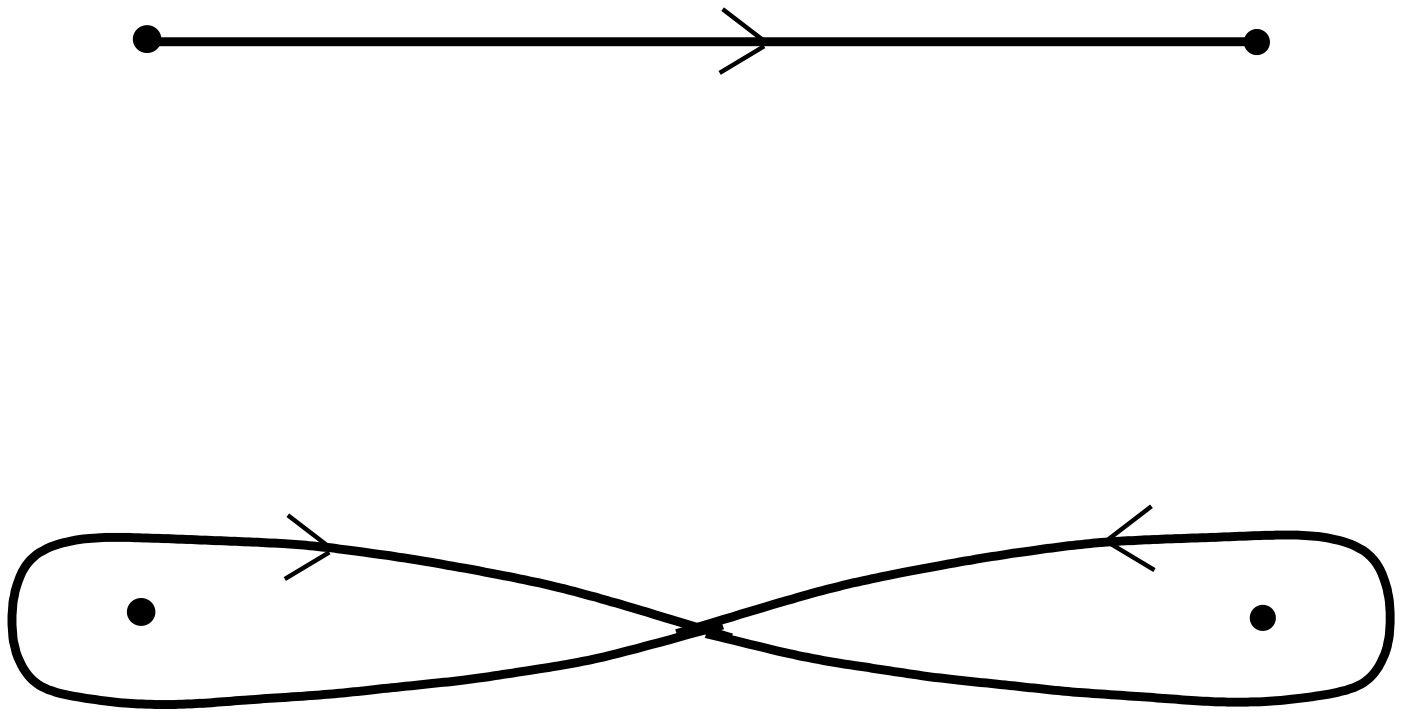
\includegraphics[width=3.5in]{figs/Fig07.png}
 \end{center}
\caption{\small 针 $\CC_{12}$（上）与闭合积分围道（下）的比较，后者等价于 $(1-q^{-1})\CC_{12}$。（原稿第 63 页）}
 \label{compare}
\end{figure}

把针与描述 BPZ 共形块时常用的闭合围道（如图~\ref{compare} 所示）作比较是很有意思的。如图所示，这些围道在同调意义下等价于针乘以一个 $q$ 的 Laurent 多项式。从 Stokes 矩阵的角度看，它们并不像针那样初等。

\subsubsection{有对称性破缺时的单个初级场}\label{onesym}


\begin{figure}
 \begin{center}
     % >>> 原文图 8（原稿第 63 页）
  
\includegraphics[width=3.5in]{figs/Fig08.png}
 \end{center}
\caption{\small 这条平行于实轴的射线，是存在对称性破缺、且只有一个最小荷初级场时的 Lefschetz 针。（原稿第 63 页）}
 \label{linel}
\end{figure}
另一个只有一个临界点的基本例子出现在存在对称性破缺、并且只有一个 $k=1$ 退化场与一个 Bethe 根的情形。Bethe 方程读作
\begin{equation}
\frac{1}{w - z} =c  \qquad c = - \frac{2 \ca}{\zeta}.
\end{equation}
于是 $w=z + \frac{1}{c}$。为方便起见，我们取常数 $c$ 为实的正数。针再次（图~\ref{linel}）与最自然的积分链 $\CC$ 重合，后者沿一条从 $z$ 出发、平行于正实轴且经过 $w$ 的射线。这个例子说明，存在对称性破缺时，积分链可以终止于无穷远。我们刚刚描述的那条链无法用等价的紧致链替代。

% [Tutor Note: 物理图像] 无对称性破缺时，针的端点只会落在 $w_i\to z_a$（即轻场所在处）；对称性破缺（无穷远处引入非正则奇点）额外提供了 $w\to\infty$ 这一“逃逸出口”，于是同一临界点的针可以终止于无穷远。这正是本小节的要点：紧致围道在同调中不再足以张成整个（扭化）相对同调，必须保留非紧链。

\subsection{两个临界点}\label{twoc}
接下来我们考虑只有一个 Bethe 根 $w$、却有两个临界点的例子。这出现在存在对称性破缺时两个 $k=1$ 初级场的情形，或无对称性破缺时三个此类初级场的情形。

\begin{figure}
 \begin{center}
     % >>> 原文图 9（原稿第 64 页）
  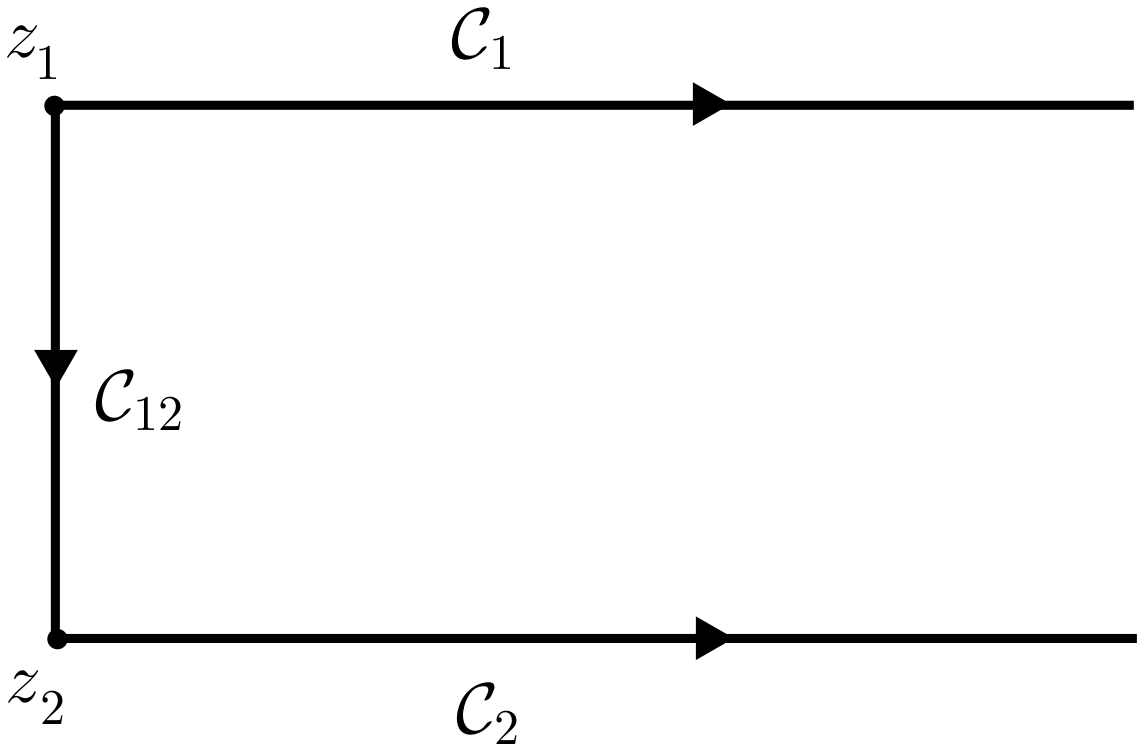
\includegraphics[width=3in]{figs/Fig09.png}
 \end{center}
\caption{\small 链 $\CC_1$、$\CC_2$ 与 $\CC_{12}$。（原稿第 64 页）}
 \label{cyclesonetwo}
\end{figure}
   % §5  从编织针到自由场积分
\subsubsection{第一个例子}\label{twop}

我们首先考虑存在对称性破缺时两个初级场的情形。记这两个初级场的位置为 $z_1$ 与 $z_2$，并继续假定对称性破缺参数 $c$ 为正。只要 $z_1-z_2$ 不是实数，就存在一组对称选取的基本积分链 $\CC_a$，$a=1,2$：它们是从 $z_a$ 出发、平行于正实轴的射线。差 $\CC_1 - \CC_2= \CC_{12}$ 是从 $z_1 $ 到 $z_2$ 的线段。参见图~\ref{cyclesonetwo}。这三条链中的任意两条都可以成为针，取决于 $c$ 与 $z_1 - z_2$ 的相对大小。由于针始终只有两个，三条链 $\CC_1$、$\CC_2$ 与 $\CC_{12}$ 绝不可能同时都是针。

在这个简单的例子里，我们已经具备了一般辫群表示的基本要素。基本操作是交换两个 $z_a$，既可以顺时针也可以逆时针。我们从两个 $z_a$ 虚部互不相同的构型出发，这样各 $\CC_a$ 都良定义。不妨把 $z_a$ 的实部取为零。我们希望沿 $\CC_1$、$\CC_2$ 与 $\CC_{12}$ 定义 $\W$ 的分支，使得 $\CC_{12}=\CC_1-\CC_2$ 成立。在 $\CC_{12}$ 上任取 $\W$ 的一个分支，再在 $\CC_1$ 与 $\CC_2$ 上定义 $\W$，使它在 $\CC_1$ 与 $\CC_{12}$ 的唯一交点处、或在 $\CC_2$ 与 $\CC_{12}$ 的唯一交点处与前者一致。这就保证了 $\CC_{12}=\CC_1-\CC_2$。虽然 $\CC_1$ 与 $\CC_2$ 并不相交，但我们可以把它们稍作形变，使它们在右侧远处的某个参考点相遇，于是 $\W$ 的两个值在该参考点处一致。（这可由下述事实保证：可以把 $\W$ 定义为在以 $\CC_1$、$\CC_2$ 与 $\CC_{12}$ 为界的半无限矩形内单值。）

% [Tutor Note: 含糊点拨] 作者说“这可由……单值保证”而略去论证，实质是：$\CC_1$、$\CC_2$ 与“无穷远处的连接段”围成的半无限矩形内 $\W$ 没有临界点，故沿该矩形边界一周 $\W$ 的单值性成立；令无穷远处的连接段收缩，即得两个参考点处 $\W$ 的取值相等。若该矩形内存在临界点，这一论证失效，正是后文 $|Z|<<1$ 时出现额外临界点的原因。

设 $\mathrm{Im}\,( z_1-z_2)>0$。那么我们可以用两种方式穿到 $\mathrm{Im}\,( z_1-z_2)<0$，即让 $z_1$ 从 $z_2$ 的左侧或右侧绕过。这两个操作互为逆操作，因此详细考察其中一个就够了。若 $z_1$ 从 $z_2$ 的右侧绕过，则 $\CC_1$ 作为一条平行于正实轴的射线连续演化。另一方面，$\CC_2$ 则不然。我们可以改用 $\CC_{12}$，它被连续地定义为从 $z_1$ 到 $z_2$ 的线段。在 $\CC_1$ 与 $\CC_{12}$ 这组基下，这一编织操作是对角的：我们只需追踪 $\W$ 的分支与链的取向。我们想把最终结果用 $\CC_1$ 与 $\CC_2$ 的基来表达。

在半编织中，$\CC_1$ 乘以因子 $q^{-\frac{1}{4}}$：$z_1$ 被顺时针地绕 $z_2$ 输运，而参考点没有显著移动。半编织之后，我们把 $\CC_1$ 重新命名为 $\CC_2$：
\begin{equation}\label{elfin}
\CC_1 \to q^{-\frac{1}{4}} \CC_2.
\end{equation}

% [Tutor Note: 易错点] 这里指数是 $-1/4$，来源是超势中的 $-\frac12\log(z_1-z_2)$ 项：$z_1$ 顺时针绕过 $z_2$ 半圈时，$z_1-z_2$ 顺时针转过 $\pi$，故 $\log(z_1-z_2)$ 改变 $-i\pi$，于是 $-\frac12\log(z_1-z_2)$ 改变 $+\frac{i\pi}{2}$，$\exp(\W/b^2)$ 乘以 $e^{\pi i/(2b^2)}=q^{-1/4}$（用 $q=e^{-2\pi i/b^2}$ 检验）。若把编织方向取反（逆时针），该因子及其后所有公式的指数符号都要整体翻转；这正是下文 (\ref{zolt}) 与 (\ref{cmono}) 相比指数符号相反的原因（作者已说明两次推导的编织方向相反）。

\begin{figure}
 \begin{center}
     % >>> 原文图 10（原稿第 65 页）
  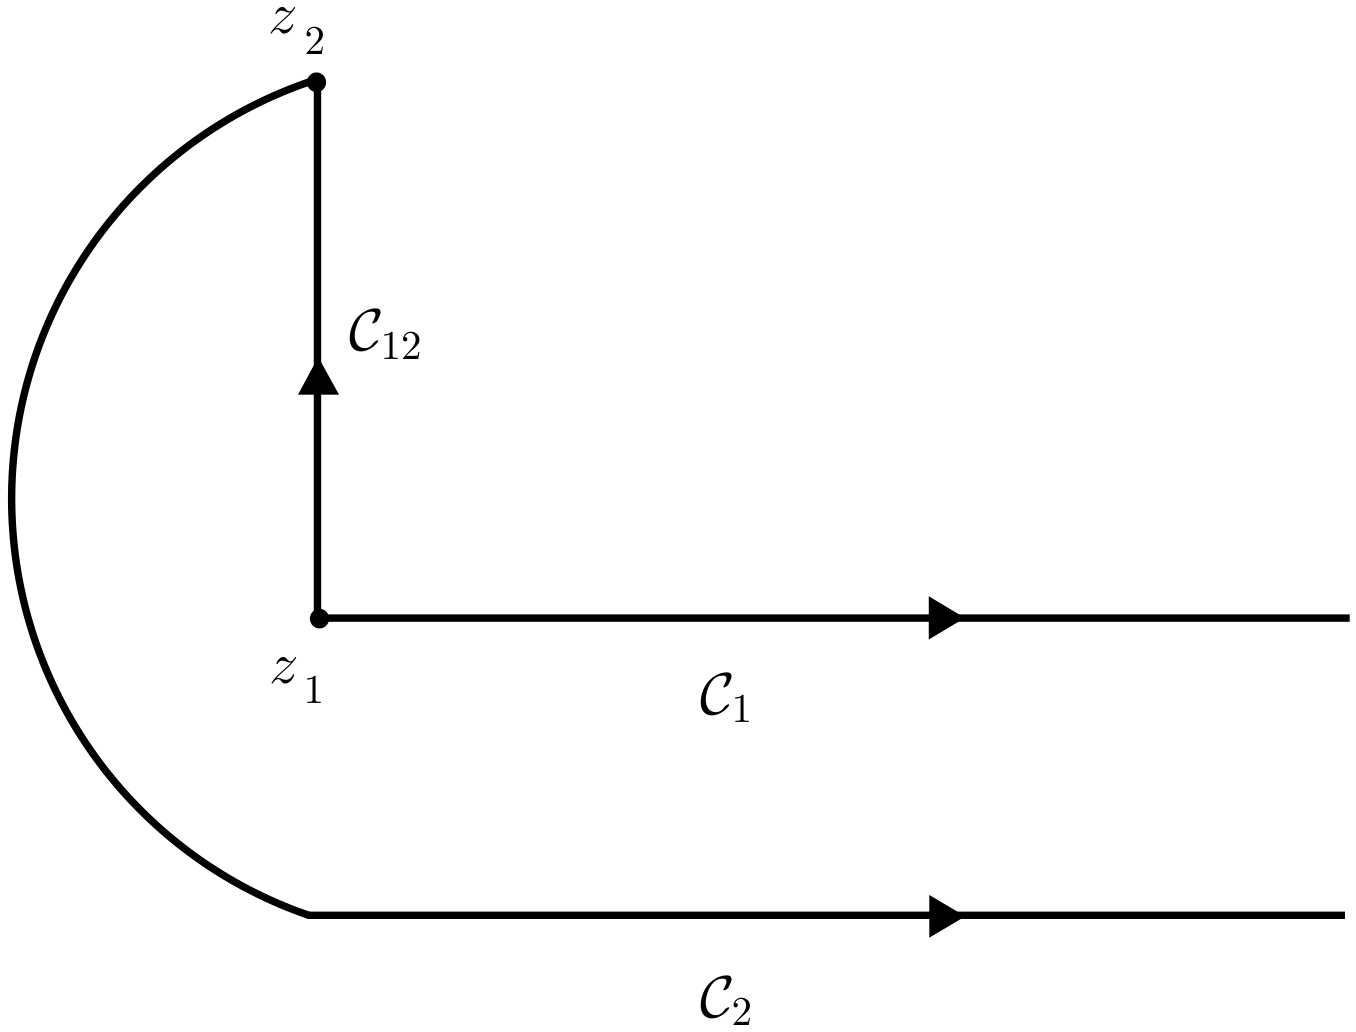
\includegraphics[width=3.5in]{figs/Fig10.png}
 \end{center}
\caption{\small 一次编织操作之后的链 $\CC_1$、$\CC_2$ 与 $\CC_{12}$。（原稿第 65 页）}
 \label{cyclesonetwob}
\end{figure}

\begin{figure}
 \begin{center}
     % >>> 原文图 11（原稿第 66 页）
  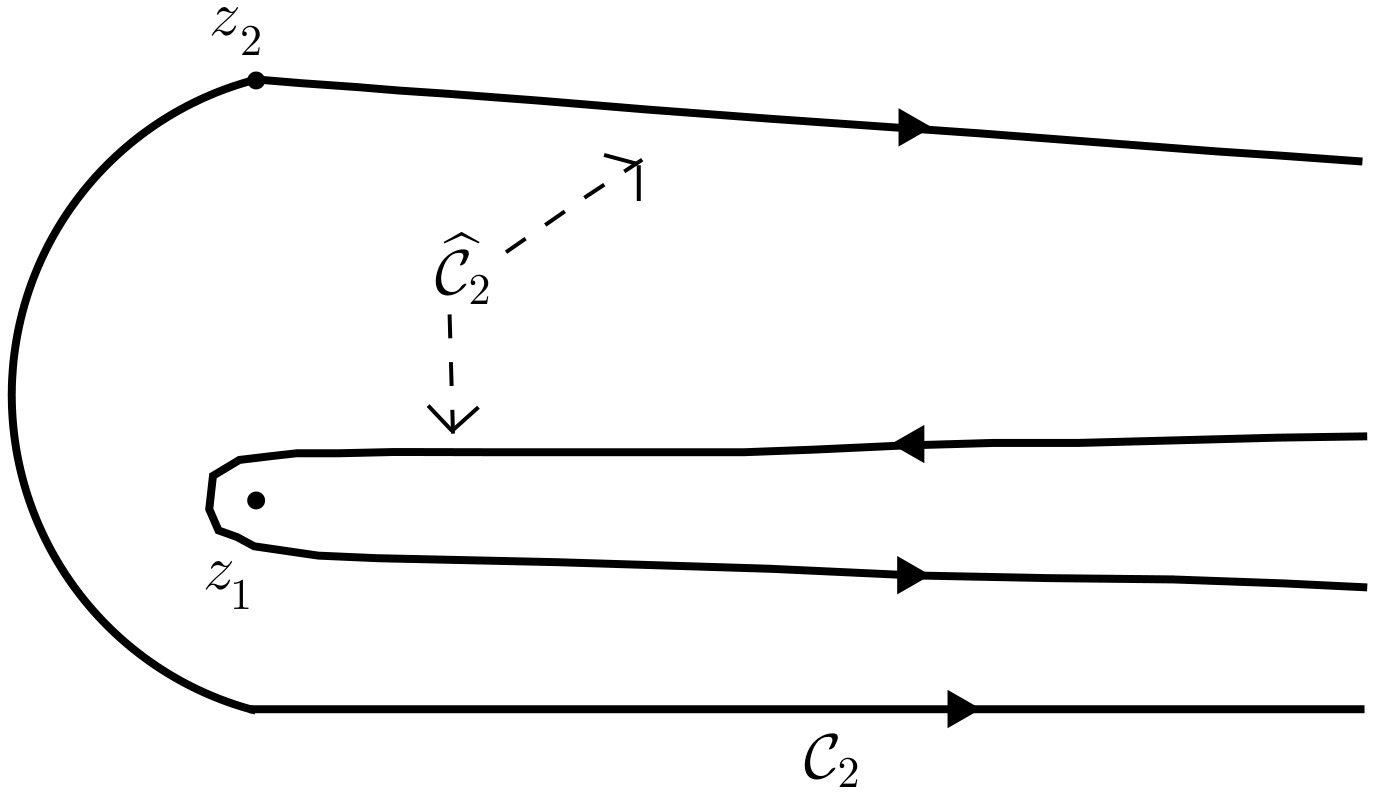
\includegraphics[width=3.5in]{figs/Fig11.png}
 \end{center}
\caption{\small 编织操作之后的链 $\CC_2$ 是照图~\ref{cyclesonetwob} 复制而来的：它从 $z_2$ 出发，从 $z_1$ 下方弯向左侧，然后通向 $\mathrm{Re}\,z=\infty$。它在同调意义下等价于图中标记为 $\widehat\CC_2$ 的锯齿形链：后者从 $z_2$ 出发，先径直通向 $\mathrm{Re}\,z=\infty$，再折返绕过 $z_1$，最后又回到 $\mathrm{Re}\,z=\infty$。于是 $\widehat\CC_2$ 是三段之和，每一段都通向或来自 $\mathrm{Re}\,z=\infty$；每一段都等价于 $q$ 的某个幂次乘以基本链 $\CC_1$ 或 $\CC_2$（即从 $z_1$ 或 $z_2$ 出发、平行于正 $z$ 轴的射线）。（原稿第 66 页）}
 \label{cyclesonetwoc}
\end{figure}

另一方面，$\CC_2$ 变成图~\ref{cyclesonetwob} 中的链。它可以形变为三段之和，这三段锯齿般地往返于 $\mathrm{Re}\,z=\infty$，如图~\ref{cyclesonetwoc} 所示。三段中的每一段都等价于 $q$ 的某个幂次乘以原链 $\CC_1$ 与 $\CC_2$ 之一。正如 (\ref{elfin}) 那样，其中一段（在再一次交换 $\CC_1$ 与 $\CC_2$ 的标号之后）是 $q^{-\frac{1}{4}} \CC_2$。另外两段则是 $-q^{-\frac{1}{4}} \CC_2$ 与 $q^{-\frac{1}{4}} \CC_1$ 在某个覆盖变换下的像。因此编织变换为
\begin{equation}
\CC_2 \to q^{-\frac{1}{4}} \CC_2-  q^{\frac{3}{4}} \CC_2 + q^{\frac{3}{4}} \CC_1.
\end{equation}

注意，在这些变换规则下，
\begin{equation}\label{zolt}
\CC_{12} \to -  q^{\frac{3}{4}} \CC_{12}.
\end{equation}
这与我们在式 (\ref{cmono}) 中得到的结果相同（指数的符号相反，因为在推导 (\ref{zolt}) 时我们是让 $z_1$ 顺时针地绕 $z_2$ 编织的）；对称性破缺并不影响下述事实：$\CC_{12}$ 代表两个退化场融合为恒等场的共形块。编织矩阵的本征值为 $-  q^{\frac{3}{4}}$ 与 $q^{-\frac{1}{4}}$，它们对应于两个可能的融合道。线性组合 $\CC_1 + q^{-1} \CC_2$ 的变换为
\begin{equation}
\CC_1 + q^{-1} \CC_2 \to q^{-\frac{1}{4}} (\CC_1 + q^{-1} \CC_2).
\end{equation}
因此它代表动量为 $-b$ 的道中的融合。

% [Tutor Note: 易错点] 两个本征值 $-q^{3/4}$ 与 $q^{-1/4}$ 分别对应恒等道（$\CC_{12}$）与动量为 $-b$ 的道（$\CC_1+q^{-1}\CC_2$）。校验可用两个不变量：在基 $(\CC_1,\CC_2)$ 下，由变换规则读出的迹为 $q^{-1/4}-q^{3/4}$、行列式为 $-q^{1/2}$，恰好等于 $(-q^{3/4})+q^{-1/4}$ 与 $(-q^{3/4})(q^{-1/4})$。注意恒等道的本征值带负号且指数为 $+3/4$；与 (\ref{cmono}) 比较时须把编织方向反过来，符号与指数才都会对上。

现在，$\CC_1$ 与 $\CC_2$ 的其他归一化选择在各种情形下可能更自然地出现。若改变 $\CC_1$ 与 $\CC_2$ 之间的相对归一化，例如令 $\tilde \CC_1 = q^{-s/2} \CC_1$ 与 $\tilde \CC_2 = q^{s/2} \CC_2$，则可以得到编织公式
\begin{equation}\label{furthox}
B_{12} :~~ \tilde \CC_1 \to q^{-s-\frac{1}{4}} \tilde \CC_2
\qquad   \tilde \CC_2 \to \left( q^{-\frac{1}{4}} -  q^{\frac{3}{4}} \right)
\tilde \CC_2 + q^{s+\frac{3}{4}} \tilde \CC_1.
\end{equation}
我们马上就会发现 $s=-\frac{1}{2}$ 这一选择很有用，因此此后每当写 $\tilde \CC_a$ 时，我们都采用该 $s$ 值。

\begin{figure}
 \begin{center}
     % >>> 原文图 12（原稿第 67 页）
  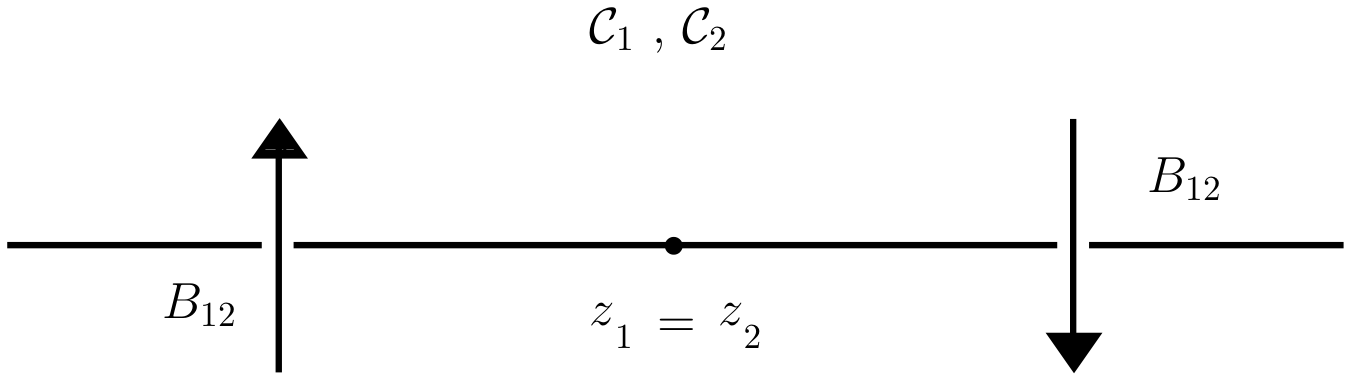
\includegraphics[width=3.5in]{figs/Fig12.png}
 \end{center}
\caption{\small 链 $(\CC_1,\CC_2)$（定义为从 $z=z_1$ 或 $z_2$ 出发、沿 $\mathrm{Re}\,cz$ 方向的射线）为同调提供了一个局部基，但穿越使 $Z=c(z_1 - z_2)$ 为实数的直线时，链的定义会跳跃一个编织矩阵 $B_{12}$。（原稿第 67 页）}
 \label{braida}
\end{figure}

各 $\CC_a$ 作为 $c(z_1 - z_2)$ 的函数的行为如图~\ref{braida} 所示。当 $c(z_1-z_2)$ 为实数时，各 $\CC_a$ 不再是良定义的。在这个非常简单的例子里，沿 $\CC_a$ 的积分可以显式地用熟知的函数表示：
\begin{align}
\I_a &= \oint_{\CC_a} (w-z_1)^{\frac{1}{b^2}}(w-z_2)^{\frac{1}{b^2}}
(z_1-z_2)^{-\frac{1}{2b^2}} e^{\frac{c z_1}{2} + \frac{c z_2}{2} - c w} \d w \cr &= c^{-1 - \frac{3}{2 b^2}} \oint_{\CC_a} (W-Z)^{\frac{1}{b^2}}W^{\frac{1}{b^2}}Z^{-\frac{1}{2b^2}} e^{\frac{Z}{2} - W} \d W 
\end{align}
这里我们定义了 $W = c(w-z_2)$ 与 $Z = c(z_1 - z_2)$。这个积分可以显式地用 Bessel 函数写出。沿 $\CC_1$ 与 $\CC_2$ 的积分给出大 $Z$ 下具有特定渐近行为的一组 Bessel 函数基，而编织矩阵 $B$ 捕捉的正是 Bessel 函数的 Stokes 现象：
\begin{align}
\I_1 &= \frac{1}{\sqrt{\pi } c^{1 + \frac{3}{2 b^2}}} Z^{\frac{1}{2 b^2}+\frac{1}{2}} \Gamma \left(1+\frac{1}{b^2}\right)
   K_{\frac{1}{2}+\frac{1}{b^2}}\left(\frac{Z}{2}\right) \cr 
   \I_2 &= \frac{q^{1/4}}{\sqrt{\pi } c^{1 + \frac{3}{2 b^2}}} Z^{\frac{1}{2 b^2}+\frac{1}{2}} \Gamma \left(1+\frac{1}{b^2}\right)
   K_{\frac{1}{2}+\frac{1}{b^2}}\left(-\frac{Z}{2}\right) 
\end{align}

% [Tutor Note: 省略证明] 从第一式到第二式（$W,Z$ 的替换）并不只是变量替换：$e^{\frac{c z_1}{2}+\frac{c z_2}{2}-cw}$ 是超势的指数化形式，代入 $W=c(w-z_2)$ 时会产生 $c$ 的幂次因子 $c^{-1-\frac{3}{2b^2}}$，其中 $-1$ 来自 $\d w=c^{-1}\d W$，$-\frac{3}{2b^2}$ 来自三个 $W,Z$ 因子的组合幂次。作者略去了这一步的幂次记账；若漏掉 $c$ 的幂，Bessel 表达式前的系数就会与原文差一个 $c$ 因子。

在大 $Z$ 极限下，沿 $\CC_a$ 的积分由 $w$ 靠近 $z_a$ 的区域所主导。取对数的一个分支使超势中对数之和在 $w$ 接近 $z_1$（或 $z_2$）时趋于 $\frac{1}{4} \log(z_1 - z_2)^2$，这样做是有用的。这与 $s=-\frac{1}{2}$ 时 $\CC_a$ 与 $\tilde \CC_a$ 之间的归一化改变相同。在强对称性破缺时，$\tilde \CC_a$ 这组基会很有用。在此基下
\begin{equation}\label{nurth}
B_{12} := \tilde \CC_1 \to q^{\frac{1}{4}} \tilde \CC_2  \qquad   \tilde \CC_2 \to \left( q^{-\frac{1}{4}} -  q^{\frac{3}{4}} \right) \tilde \CC_2 + q^{\frac{1}{4}} \tilde \CC_1.
\end{equation}

到目前为止，我们所用的链 $\CC_1$、$\CC_2$ 与 $\CC_{12}$ 都是凭观察就能看出的。让我们把这些链与针作比较。含两个 $z$ 与一个 $w$ 的 Bethe 方程为
\begin{equation}
\frac{1}{w - z_1} + \frac{1}{w - z_2} =c
\end{equation}
它有两个解。

有两个值得关注的区域。若 $|Z|>>1$，则临界点近似为 $w = z_a + 1/c$，$a=1,2$。对这两个临界点中的每一个，假定 $c>0$ 且 $\mathrm{Re}\,Z=0$，则 $w-z_1$ 与 $w-z_2$ 的实部都为正；因此在定义 $\W$ 时，自然地选取 $\log(w-z_1)$ 与 $\log(w-z_2)$ 的分支使其虚部被 $\pm \pi/2$ 界定。这样定义的针与我们上面定义的 $\tilde \CC_a$ 重合（而不与 $\CC_a$ 重合）。这一选择的优点在于，它可以自然地推广到存在对称性破缺、包含许多场的一般情形，我们将在第~\ref{genpicture}~节讨论该情形。若 $|Z|<<1$，则我们有近似临界点 $w = \frac{1}{2}(z_1 + z_2)$ 与 $w=2/c$。第一个临界点位于两个 $z_a$ 之间，与之相伴的针是 $\CC_{12}$。第二个临界点在 $\mathrm{Re}\, Z >0$ 时与 $\CC_1$ 相伴，否则与 $\CC_2$ 相伴。

% [Tutor Note: 物理图像] 两种区域给出两套不同的“自然基”：$|Z|>>1$（弱对称性破缺、两场相距很远）时针是两条平行射线 $\tilde\CC_a$；$|Z|<<1$（强破缺）时针是连接两 $z_a$ 的线段 $\CC_{12}$ 加上一条射线。针的定义随参数连续变化，但"哪两条链是针"这一信息在穿过 Stokes 墙时发生跳变（墙自两临界点重合的 $Z=\pm 2i$ 出发）——这正是图~\ref{braidb} 的物理含义。

\begin{figure}
 \begin{center}
     % >>> 原文图 13（原稿第 68 页）
  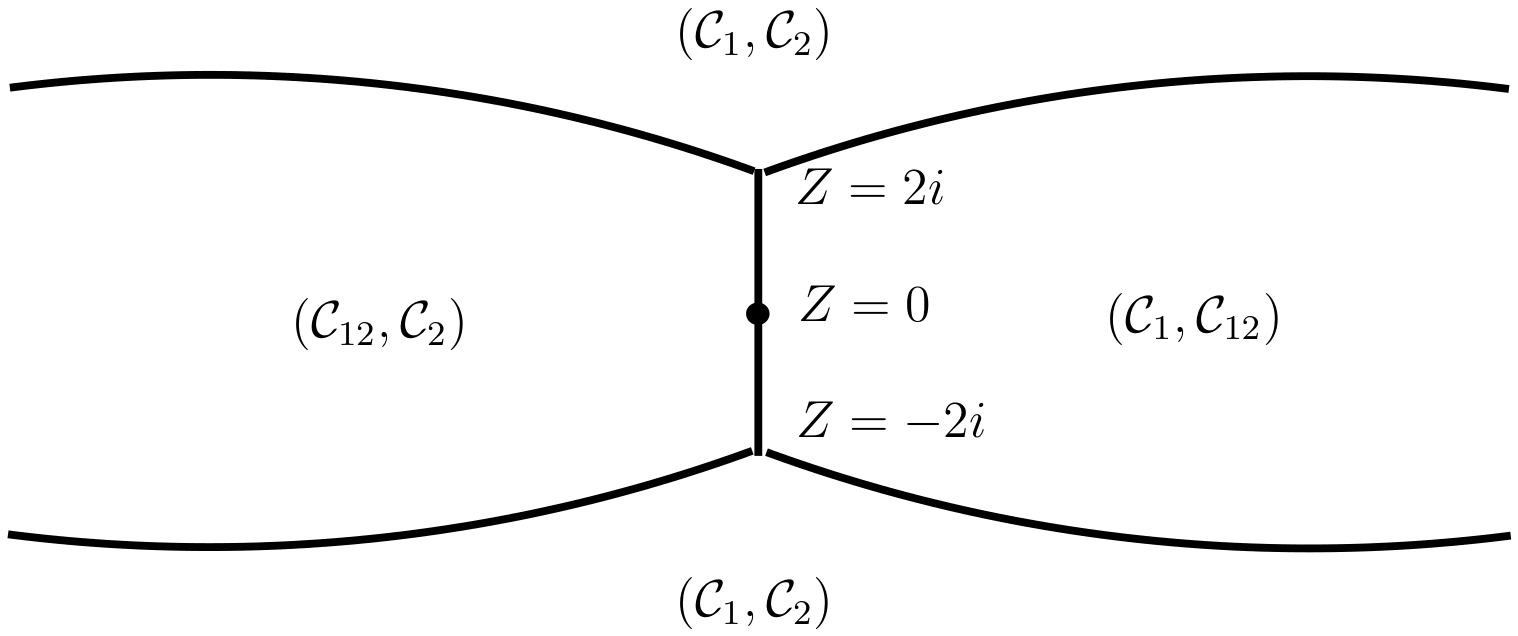
\includegraphics[width=4in]{figs/Fig13.png}
 \end{center}
\caption{\small $c(z_1 - z_2)$ 平面中 Stokes 墙的分布与针基。（原稿第 68 页）}
 \label{braidb}
\end{figure}

我们在图~\ref{braidb} 中画出针系的 Stokes 墙。参数空间中存在这样的区域：在其中针基由 $\CC_1$、$\CC_2$ 与 $\CC_{12}$ 中的任意两条构成（至多相差超势分支的选择）。区域两两沿 Stokes 墙相接，三个区域则在两个临界点重合的点 $Z=\pm 2i$ 处相遇。这是一般性特征；在这类一般问题中，总会存在复余维 $1$ 的轨迹，在其上两个临界点重合。在垂直于该轨迹的平面内，$\W$ 可以用单变量 $w$ 的简单三次函数 $\W = w^3 + \delta w$（带参数 $\delta$）来模拟；该函数有两个临界点，它们在 $\delta=0$ 时重合，此处三条 Stokes 墙相交。局部的 Stokes 行为是普适的；它对应于 Airy 函数的行为。

% [Tutor Note: 数学工具] $\W=w^3+\delta w$ 是两临界点碰撞的普适模型（余维 1 的 $A_2$ 型奇点）：$\delta=0$ 时三重临界点处有三条 Stokes 墙交汇，其局部构型由 $\W=w^3$ 的相位决定，相关 Stokes 乘子由 Airy 函数的渐近展开固定。记住这一点可省去逐题计算：任何"两临界点靠近"的局部问题，其编织矩阵的普适部分都是 Airy/Stokes 乘子，差别只在全局的 $q$ 幂次。

正如我们在第~\ref{fromth}~节的一般讨论中所解释的，$b\to 0$ 时积分的渐近行为在针基下最为清晰。就当前问题而言，图~\ref{braidb} 已经抓住了相关信息。图中共有四个区域：上下两个区域对应于我们在 $|Z|>>1$ 极限下看到的针系，中间两个区域对应于我们在 $|Z|<<1$ 极限下看到的针系。

\begin{figure}
 \begin{center}
     % >>> 原文图 14（原稿第 68 页）
  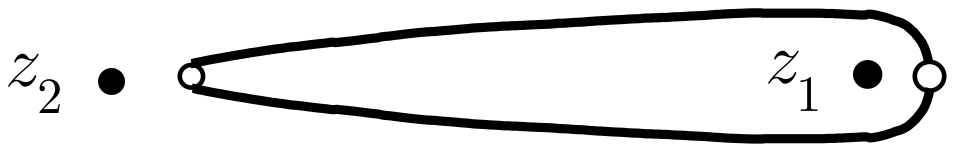
\includegraphics[width=2.5in]{figs/Fig14.png}
 \end{center}
\caption{\small 从 $z_2$ 附近的临界点（空心圆点）流向 $z_1$ 附近临界点（空心圆点）的两条 Morse 流。这两条流发生在略有不同的 ${\mathrm{Im}}\,Z$ 值处。（原稿第 68 页）}
 \label{braidc}
\end{figure}

公式 (\ref{furthox}) 或 (\ref{nurth}) 描述了编织矩阵 $B_{12}$，它把图~\ref{braidb} 顶部（此处的针是 $\CC_1$ 与 $\CC_2$）的区域与底部（此处的针同样是 $\CC_1$ 与 $\CC_2$）的区域联系起来。这个计算是我们凭观察作出的，而不是通过分析 Stokes 线得到的。在推导 (\ref{nurth}) 时，我们假定 $z_1$ 沿顺时针方向绕 $z_2$ 走了半圈；这相当于在图~\ref{braidb} 中取 $\mathrm{Re}\,Z>0$ 而从顶部移到底部。由图~\ref{braidb} 可见，在这一过程中我们会穿过两条 Stokes 线。这意味着，在针基下，编织矩阵 $B_{12}$ “分解”为两个基本操作的序列，每个基本操作与一条 Stokes 线相伴。每个基本操作都涉及一个梯度流：Bethe 根 $w$ 从 $z_2$ 右侧邻近的临界点流向 $z_1$ 右侧邻近的临界点。这样的流有两条，区别在于 $w$ 从 $z_1$ 上方还是下方经过。这两条流发生在略有不同的 $\mathrm{Im}\,Z$ 值处，如图~\ref{braidc} 所示。在式 (\ref{nurth}) 的公式 $B_{12}\tilde C_2=
(q^{-1/4}-q^{3/4})\tilde C_2+q^{1/4}\tilde C_1$ 中，右端的项 $q^{1/4}\tilde C_1$ 仅来自形式单值性，而另外两项则来自两个梯度流解的贡献。

% [Tutor Note: 易错点] “形式单值性”（formal monodromy）与梯度流贡献的分解是本题最易混淆处：$q^{1/4}\tilde C_1$ 项不来自任何实际流，算的是绕 $Z=0$ 一圈时对数分支的解析延拓；而 $(q^{-1/4}-q^{3/4})\tilde C_2$ 中的两项分别对应穿过两条 Stokes 线时的跳变。若把三项统统当作“流的贡献”，就会错误地预测应有三个临界点或三条流。核对时可用 $b\to0$ 的鞍点图像：只有真实临界点才给出指数小的贡献。

在小 $Z$ 区域，绕 $Z=0$ 的编织在针基下由三角矩阵表示：$\CC_{12}$ 是一个本征向量。这一事实有一般的理由：无论在 $Z \to 0$ 极限还是在 $b \to 0$ 极限下，沿 $\CC_{12}$ 的积分都小于沿任何其他链的积分。在任一极限下，沿 $\CC_{12}$ 的积分都由通常的鞍点近似控制，而与 $\CC_{12}$ 相伴的临界点正是 Morse 函数取最小值的那个临界点。因此 $\CC_{12}$ 必定是单值性的本征向量。对于任意数目的 $z$ 与 $w$，那些在某对非常接近的 $z_a$ 之间夹有一个 $w$ 的针集合，张成共形块的“小”本征空间，其中动量为 $- \frac{1}{2b}$ 的两个退化场融合为恒等场。

\subsubsection{第二个例子}\label{sec}

第二个有两个临界点的例子出现在有三个最小荷奇异磁单极子与一个 Bethe 根 $w$ 的情形。把奇异磁单极子置于 $z_1,z_2,z_3$，此时有三个显然可能的积分链：连接 $z_a$ 与 $z_b$ 的直线路径（对任意 $a,b$）。我们可以选取超势的分支，使得这三条链之和为零。

若这三点不共线，则上述定义是有意义的。此时 $z_a$ 的参数空间被分成两半：或者 $z_1$、$z_2$、$z_3$ 构成正向的三角形，或者构成负向的三角形。我们把两种情形下的三条自然链都记为 $\CC_{ab}^\pm$。于是
\begin{equation} \label{skeinc}
\CC^+_{12} + \CC^+_{23} + \CC^+_{31} = 0 \qquad \CC^-_{12} + \CC^-_{23} + \CC^-_{31} =0
\end{equation}
但这两组基在 $z_a$ 共线的轨迹两侧以有趣的方式相联系。

这样的轨迹有三条，每条对应三个 $z_a$ 中某一个从另外两个之间穿过。例如，若 $z_2$ 从 $z_1$ 与 $z_3$ 之间穿过，则 $\CC^+_{12}$ 与 $\CC^+_{23}$ 同 $\CC^-_{12}$ 与 $\CC^-_{23}$ 的关系仅仅是 $\W$ 的分支改变，而 $\CC^+_{13}$ 的变换则由 (\ref{skeinc}) 推出。

Bethe 方程
\begin{equation}\label{polz} \frac{1}{w-z_1}+\frac{1}{w-z_2}+\frac{1}{w-z_3} =0 \end{equation}
等价于关于 $w$ 的一个二次方程，因此它有两个解，对应于两个独立的针。这些针等价于连接某一对 $z$ 的路径中的两条，但具体出现哪两对取决于 $z$ 的选取。若各 $z$ 共线，则 Bethe 根位于相邻 $z$ 之间的线段上，而针与这些线段重合。例如，若 $z_2$ 位于 $z_1$ 与 $z_3$ 之间，则两个针是 $\CC^\pm_{12}$ 与 $\CC^\pm_{23}$（至多相差 $q$ 的幂次）。

与通常一样，连接 $z_a$ 与 $z_b$ 的针对应于相应的两个退化场融合为恒等场的共形块。关系式 (\ref{skeinc}) 对应于三个初级场中取两个融合为恒等场的三种不同方式之间的基本“拆接关系”（skein relation）。换言之，只要 $z_a$ 与 $z_b$ 靠得很近，就存在一条连接它们的针，它是 $z_a$ 与 $z_b$ 之编织的本征向量，而该编织矩阵是三角的。

\begin{figure}
 \begin{center}
     % >>> 原文图 15（原稿第 70 页）
  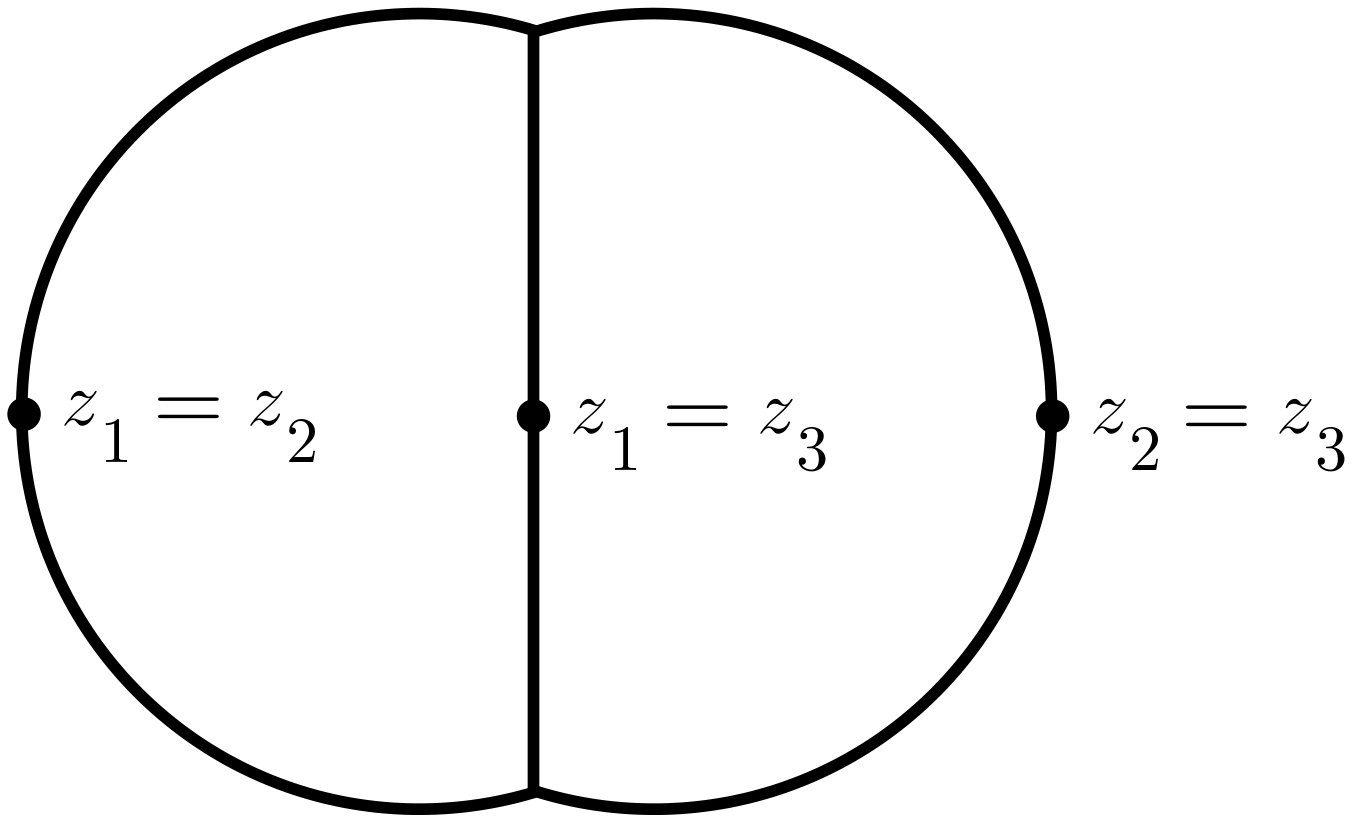
\includegraphics[width=3.5in]{figs/Fig15.png}
 \end{center}
\caption{\small 以 $z_1$、$z_2$、$z_3$ 为顶点的三角形形状空间中的 Stokes 墙分布。（原稿第 70 页）}
 \label{stok}
\end{figure}

我们在图~\ref{stok} 中画出这些 Stokes 墙。积分 $I_{ab}$ 可以容易地用超几何函数求出。

\subsection{最后一个例子}\label{fin}
还有一个例子既有启发性，又对理解一般图像很有用。这就是两个荷为 $1$ 的 $z_a$ 伴随着两个 $w_i$ 的情形。这只能在存在复对称性破缺时发生。容易看出，Bethe 方程 (\ref{normo}) 只有唯一的解。$Q$ 与 $K$ 的次数都是 $2$，因此 $P$ 的次数为 0，可以取为 1。由此得到一组线性方程，它们唯一地确定 $Q$ 中的系数。由于 Bethe 方程的解唯一，只有一个共形块，而编织 $z_a$ 时的单值性只能是乘以 $q$ 的某个函数。

% [Tutor Note: 易错点] 这里的 $P,Q,K$ 是 Bethe 拟设中用到的多项式（$Q=\prod(w-w_i)$ 等），“$\deg Q=\deg K=2$ 故 $\deg P=0$” 的计数依赖前文 (\ref{normo}) 的具体形式，不要把它当成一般结论。另外，“单值性只能是乘以 $q$ 的某个函数”之所以成立，是因为只有一个本征向量（一维表示）；若解不唯一，单值性就会是矩阵而非标量。

若 $z_1$ 与 $z_2$ 相距很远，即 $c(z_1 - z_2)$ 的绝对值很大，则 Bethe 方程的解容易描述：$w_1 \sim z_1 + 1/c$ 与 $w_2 \sim z_2 + 1/c$。存在一个显然的积分链：$w_1$ 与 $w_2$ 分别沿从 $z_1$ 与 $z_2$ 出发、朝 $c$ 方向伸向无穷的射线积分；这些射线在图~\ref{cyclesonetwo} 中被标为 $\CC_1$ 与 $\CC_2$。我们可以把这个链记为 $\CC = \CC_1 \times \CC_2$。

若 $Z = c(z_1 - z_2)$ 的虚部很大，则该问题的唯一针是 $\CC$ 的小形变。当我们形变 $Z$ 时，唯一的针会连续地形变。Morse 理论在这里相当有用：用手工验证 $\CC$ 在 $z_1$ 与 $z_2$ 编织之后回到自身是相当棘手的，因为这需要一次不能使 $\CC$ 保持简单乘积形式的围道形变；而针的演化恰好隐含地提供了这样的形变。同样，乍看之下远不明显的是，由 $w_1$ 与 $w_2$ 上的围道积分产生的共形块，会是 $Z$ 平面中具有阿贝尔单值性的简单函数。然而情形必定如此。

编织的效应在大 $c$ 下可以通过积分的鞍点估计容易地算出。在鞍点处，只要整个过程在大 $|Z|$ 下进行，$w_1 \sim z_1 + 1/c$ 与 $w_2 \sim z_2 + 1/c$ 就在整个编织过程中保持成立。$\W$ 的 Hessian 接近于单位矩阵的一个大的、与 $Z$ 无关的倍数（$\sim| c |^2$），因此大 $Z$ 下的编织相位由临界点处 $\exp(\W/b^2)$ 的取值控制。相关因子为
\begin{equation}
(z_1 - z_2)^{-b^{-2}/2} (w_1 - z_2)^{b^{-2}}(w_2 - z_1)^{b^{-2}}(w_1 - w_2)^{-2 b^{-2}} \sim (z_1 - z_2)^{-b^{-2}/2}.
\end{equation}
于是我们重新得到与两个 $z_a$ 荷为 $1$、不含 $w_i$ 的构型中相同的编织相位。

后一陈述将成为第~\ref{abdesc}~节构造有效阿贝尔描述的部分依据。在阿贝尔理论中，人们会预期两个对象的编织只依赖于它们荷的乘积。因此，两个荷均为 $-1$ 的对象（不带 $w$ 的 $z$）之间的编织，与两个荷均为 1 的对象（带 $w$ 的 $z$）之间的编织给出相同的结果。荷为 1 的对象与荷为 $-1$ 的对象之间的编织则不那么简单，因为正如我们在第~\ref{twop}~节所看到的，非平凡的梯度流会进入其中。

\subsection{存在对称性破缺的一般图像}\label{genpicture}
本节中，我们建立存在对称性破缺的一般图像。取对称性破缺参数 $c$ 为实的正数；考虑任意数目的奇异磁单极子，位于 $z_a$，$a=1,\dots,d$，以及任意数目的 Bethe 根 $w_i$，$i=1,\dots,q$。首先，我们把所有荷 $k_a$ 都取为 $1$。

我们可以手工构造一组积分链基。假定各 $z_a$ 的虚部互不相同，并按 $a'>a$ 时 $\mathrm{Im} (z_a- z_{a'}) >0$ 排序。我们定义从 $z_a$ 出发、平行于正实轴的射线 $\CC_a$。

我们的积分链将是乘积 $\CC_{a_1 a_2\cdots a_q} := 
\CC_{a_1} \times\CC_{a_2} \times \cdots \times \CC_{a_q}$，对应于 $q$ 个互不相同 $z$ 的每一个子集。这样得到 ${d \choose q}$ 条积分链，在大 $c$ 区域它们可以解释为针。确实，Bethe 方程
\begin{equation}
\sum_a \frac{1}{w_i - z_a} = c + \sum_{j \neq i} \frac{2}{w_i - w_j}
\end{equation}
在大 $c$ 时有近似解，其中每个 $w_i$ 近似等于 $z_{a_i}+1/c$，且当 $i\not=j$ 时 $a_i\not=a_j$。相应的针正是 $\CC_{a_1a_2\dots a_q}$。对所有 $q$ 求和，我们一共得到 $2^d$ 个临界点或共形块，正如所预期的那样。

在这组基下，辫群表示相当简单。我们让各 $z_a$ 在复平面中移动。Stokes 墙近似位于两个 $z_a$ 实部相等的轨迹处。当且仅当某个不带 $w_i$ 的 $z_a$ 从某个带 $w_i$ 的 $z_{a'}$ 右侧经过时，才会出现 Morse 流。由此产生的行为只涉及正在交叉的那两个 $z$，并且正是我们在第~\ref{twop}~节详细分析过的内容。当 $z_a$ 穿过 $z_{a'}$ 时，编织矩阵只非平凡地作用于 $\CC_a$ 与 $\CC_{a'}$（以及任何包含其中之一或两者的链 $\CC_{a_1a_2\dots a_q}$），并取与 (\ref{nurth}) 相同的形式。如图~\ref{braidc} 所示，这一过程的编织矩阵可以解释为源于一对 Morse 理论流。验证辫群关系成立是繁琐的，但却是初等的；它们理应成立。
   % §6  积分链表示的编织（前半）
\subsubsection{任意荷的退化场}\label{degany}

现在，仍在复对称性破缺的情形下，我们将放松所有 $k_a$ 都等于 $1$ 这一限制。
首先考虑单个荷为 $k$ 的 $z$，带有 $q$ 个 Bethe 根。只有当 $k \geq q$ 时 Bethe 方程才有解。
（这一点从 oper 的式 (\ref{normo}) 即可看清。）实际上，根据 Bethe 方程的理论，对给定的 $q$，解是唯一的，并且对应于唯一的针或积分链。

% [Tutor Note: 省略证明] “$k\geq q$ 由 (\ref{normo}) 即可看清”一句略去了论证：按 oper 的次数关系 $p+q=k+1$，$Q$ 的次数就是 Bethe 根数 $q$，故 $P$ 的次数为 $p=k+1-q$；当 $q>k+1$ 时该次数为负，而 $q=k+1$ 时 $P$ 退化为常数、不足以在无穷远处提供 oper 所需的领头行为，因此必须有 $q\le k$。此外“解唯一”是 Bethe 方程理论的一般结论，并非本模型特有。

\begin{figure}
 \begin{center}
     % >>> 原文图 16（原稿第 72 页）
  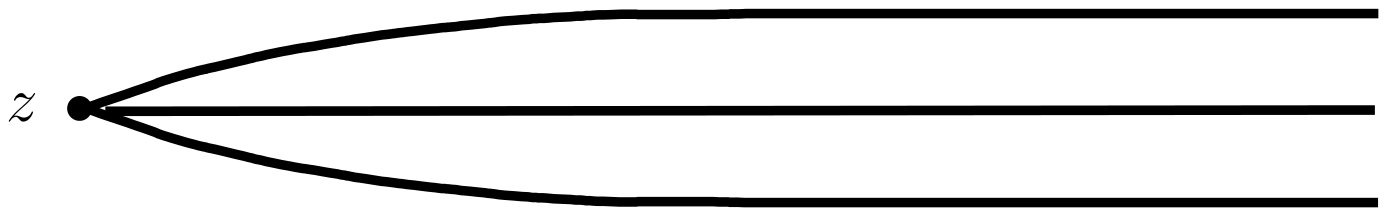
\includegraphics[width=3.5in]{figs/Fig16.png}
 \end{center}
\caption{\small 非最小荷的单个奇异磁单极子的一个积分链。（原稿第 72 页）}
 \label{thimone}
\end{figure}

\begin{figure}
 \begin{center}
     % >>> 原文图 17（原稿第 72 页）
  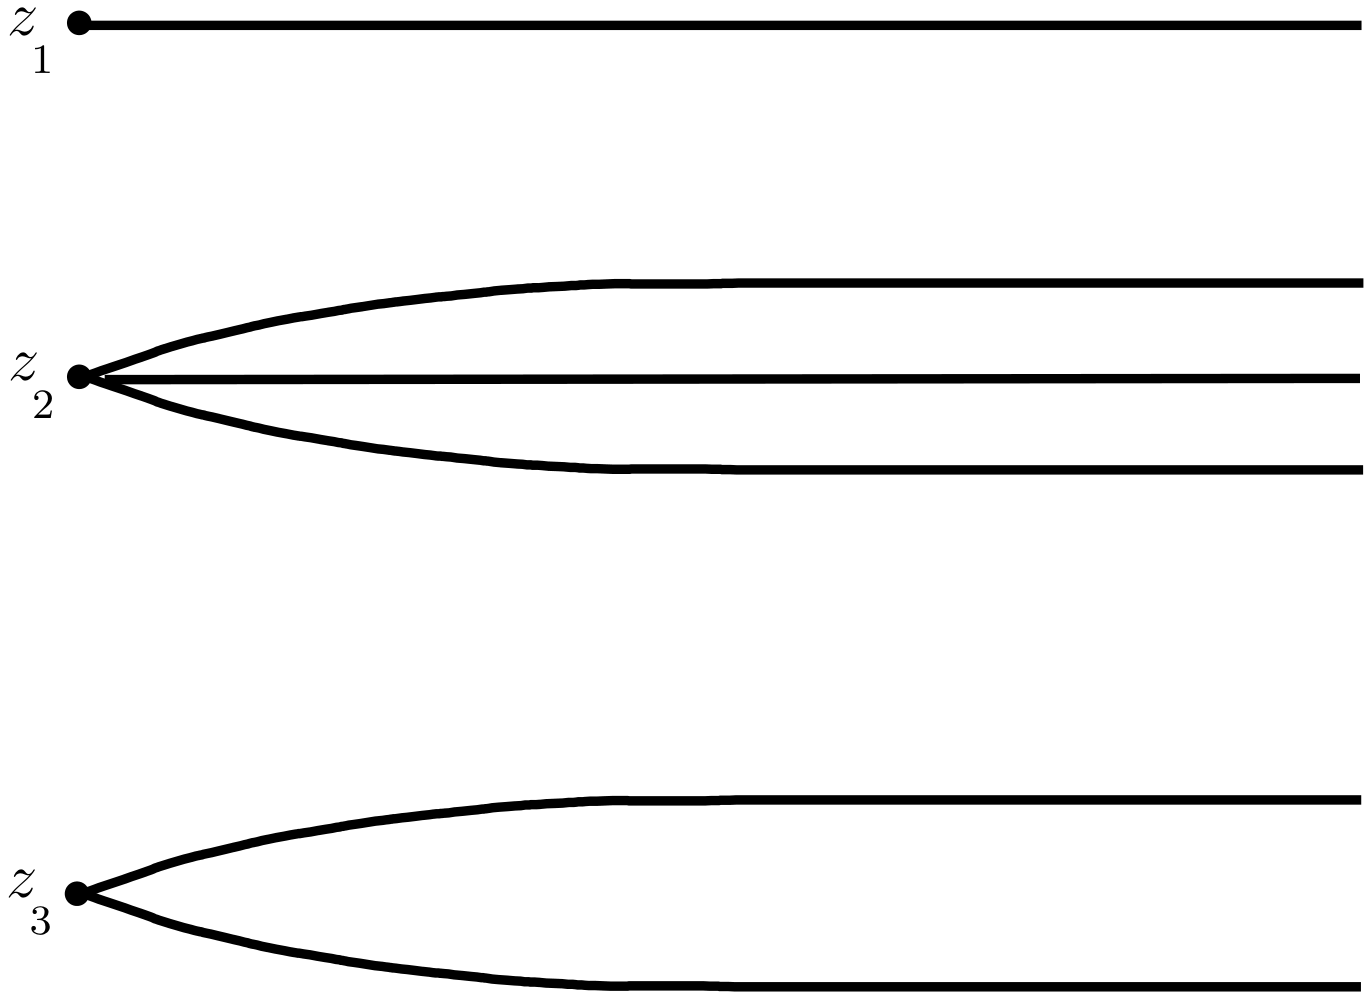
\includegraphics[width=3.5in]{figs/Fig17.png}
 \end{center}
\caption{\small 若干个非最小荷奇异磁单极子的一个积分链。对合适的 $q_a$，我们在 $z_a$ 上附着 $q_a$ 个 $w$。图中 $q_a$ 分别为 $1,3$ 与 2。（原稿第 72 页）}
 \label{thimtwo}
\end{figure}
确实，这个唯一可能的积分链 $\CC^{(q)}$ 很容易描述：把每个 $w_i$ 沿互不相同、互不相交的路径从 $z$ 积分到 $+\infty$，如图~\ref{thimone} 所示。

于是我们可以立即描述最一般情形下的积分链基：$z_a$ 的数目任意，荷为 $k_a$，而 $w_i$ 的数目 $q \leq \sum_a k_a$。对 $q = \sum_a q_a$（其中 $q_a \leq k_a$）的每一种分解方式，我们都得到一条唯一的链：对每个 $a$，把 $q_a$ 个 $w_i$ 沿互不相同、互不相交的路径从 $z_a$ 积分到 $+\infty$，如图~\ref{thimtwo} 所示。这样得到积分链 $\prod_a \CC^{(q_a)}_a$。

在强对称性破缺下（等价地说，当各 $z_a$ 沿虚轴彼此远离时），这些积分链对应于与 Bethe 方程唯一解相伴的针，其中 $q_a$ 个 $w_i$ 位于 $z_a$ 附近。原则上，在此基下导出辫群表示不存在任何障碍。

关于对任意 $k_a$ 构造辫群表示的同调方法（本质上对应于自由场实现），尽管是在没有对称性破缺的情形下，可参见文献~\cite{Ltwo}。

\subsection{关闭对称性破缺}
由于对称性破缺在简化我们的分析方面如此有用，自然就产生了一个问题：需要验证对称性破缺不会影响纽结或链环不变量的取值。

上一节对积分链的描述，只要对称性破缺参数 $c$ 非零就适用。但当 $c\to 0$ 时，我们会失去一些积分链，因为 $w_i$ 不能再趋于无穷。用 $\W$ 的临界点来说，小 $c$ 下的行为容易描述。
对小 $c$，对 Bethe 方程的每个解，Bethe 根自然地分成两个子集。其中 $q_0$ 个 Bethe 根（我们记为 $w^{(0)}_i$，$i=1,\dots,q_0$）在 $c \to 0$ 极限下保持为 $1$ 阶，而其余的 $q_\infty$ 个 Bethe 根（我们记为 $w^{(\infty)}_j,$ $j=1,\dots,q_\infty$）则为 $c^{-1}$ 阶。

在这种情况下，$w^{(0)}_i$ 所满足的 Bethe 方程可由无对称性破缺时相同数目 $w$ 的 Bethe 方程很好地近似。另一方面，$w^{(\infty)}_j$ 所满足的 Bethe 方程可由如下 Bethe 方程很好地近似：有相同数目的 $w$，并且存在单个荷为 $k_{\mathrm{eff}}=\sum_a k_a - 2 q_0$ 的 $z$。式 (\ref{ruy}) 保证 $k_{\mathrm{eff}}$ 非负，因此实际上
 \begin{equation}\label{helpful}0\leq k_{\mathrm{eff}}\leq \sum_ak_a.\end{equation}
正如我们在第~\ref{degany}~节所讨论的，若 $k_{\mathrm{eff}}\geq q_\infty$，则 $w^{(\infty)}_i$ 的 Bethe 方程有唯一解；否则无解。
对所有分解 $q=q_0+q_\infty$ 求和、对 $w^{(0)}_i$ 的 Bethe 方程的所有解求和，最后再对所有可能的 $q$ 值求和，就得到 Bethe 方程解的预期数目 $\prod_{a=1}^d (k_a+1)$。

% [Tutor Note: 易错点] $k_{\mathrm{eff}}=\sum_a k_a - 2q_0$ 中的因子 $2$ 来自 oper 定义里的平方关系 $p(z)Q(z)^2=K(z)$（见前文）：$K$ 的零点总数为 $\sum_a k_a$，而 $Q$ 以平方出现，故留在有限平面的 $q_0$ 个 Bethe 根共消耗 $2q_0$ 个零点，剩下归到无穷远的零点数为 $k_{\mathrm{eff}}$。若漏掉这个 $2$，(\ref{helpful}) 的非负性就会被误判。这一步是本节“关闭对称性破缺”论证的核心记账。

这一计数可以用对偶 $SU(2)$ 规范场论的 Wilson 算符来作如下表述。荷为 $k_a$ 的奇异磁单极子对应于 $SU(2)$ 的表示 $R_a$，其自旋为 $k_a/2$、维数为 $k_a+1$。张量积 $R=\otimes _a R_a$ 的维数为 $\prod_a(k_a+1)$。该表示可以分解为自旋 $k_{\mathrm {eff}}/2$ 的 $SU(2)$ 模的直和（其中 $k_{\mathrm{eff}}$ 受 $0\leq k_{\mathrm{eff}}\leq \sum_ak_a$ 约束，正如 (\ref{helpful}) 中那样）。以该自旋变换的态，其数目等于满足 $\sum_a k_a-2q_0=k_{\mathrm{eff}}/2$ 的 Bethe 方程解的数目（以及对所有可能的 $q$ 值）。

% [Tutor Note: 原文存疑] 此处“满足 $\sum_a k_a-2q_0=k_{\mathrm{eff}}/2$”与本节前面给出的 $k_{\mathrm{eff}}=\sum_a k_a-2q_0$ 相差一个因子 $2$：按上下文，与该自旋对应的应满足 $\sum_a k_a-2q_0=k_{\mathrm{eff}}$（即 $q_0=(\sum_a k_a-k_{\mathrm{eff}})/2$）。原文如此，疑为笔误；按铁律公式未作改动，请读者以后文的计数逻辑为准。

现在考虑各 $z_a$ 的编织。对足够小的 $c$，当穿过一条 Stokes 墙时，存在使 $q_\infty$ 变小的 Morse 流，但不存在使 $q_\infty$ 变大的这类流。原因在于，当 $c\to 0$ 时，Morse 函数 $h=\mathrm{Re}\,\W$ 在临界点处的取值随 $q_\infty$ 增大而增大。（这是因为当 $c\to 0$ 时，$h$ 的某些贡献为 $\ln(1/|c|)$ 阶。借助 (\ref{helpful}) 可以证明，$\ln(1/|c|)$ 的系数是 $q_\infty$ 的增函数。）因此，若按 $q_\infty$ 的取值把物理态空间 $\H$ 分解，则单值性矩阵是分块三角的：
\begin{equation}\label{blocks}B\sim \begin{pmatrix} *& *&* & * & * \cr  *&*&*&*&*\cr
                                                                                   0& 0 & *&* & *\cr 0&0&*&*&*\cr
                                                                         0&0&           0 & 0 & * \cr \end{pmatrix}.\end{equation}
对角块（在所给例子中秩分别为 $2,2,$ 与 1）就是在给定 $q_0=q-q_\infty$ 时、无对称性破缺情形下会有的单值性表示。

只要人们能通过取辫群表示的迹来计算纽结或链环不变量，(\ref{blocks}) 中的非对角块就不重要，因为它们对迹没有贡献。实际上，为了计算 Jones 多项式以及纽结与链环的相关不变量，除了辫群表示之外，还需要一个额外的“融合”操作：产生或湮灭一对荷相同的 $z_a$。要确保纽结不变量不受对称性破缺影响、并且在令 $c=0$ 时不发生变化，我们所需的额外信息是：融合从不涉及在无穷远处产生或湮灭任何 $w$。这一点是自然的，因为融合操作具有局域性。

\subsubsection{一处澄清}\label{clarify}

细心的读者可能注意到这一推导中有一处小小的偷换。不等式 $k_{\mathrm{eff}}\geq 0$ 是由 (\ref{ruy}) 推出的，但 (\ref{ruy}) 最初的推导基于选取 $Q$ 使其次数小于 $P$ 的次数。$c=0$ 时的 Bethe 方程当然存在不满足这一条件的解。我们凭什么可以只考虑这种情形？

设在 $c=0$ 时我们找到一对满足 oper 条件的 $P_0,Q_0$
\begin{equation}\label{opcon} P\frac{\d Q}{\d z}-\frac{\d P}{\d z}Q=K(z).\end{equation}
现在设想开启很弱的对称性破缺。oper 方程变为
\begin{equation}\label{opconz} P\frac{\d Q}{\d z}-\frac{\d P}{\d z}Q-cPQ=K(z).\end{equation}
我们希望随着 $c$ 的开启，存在一对 $(P(z;c),Q(z;c))$ 满足 (\ref{opconz})，并且 $Q$ 具有展开
\begin{equation}\label{turnox}Q(z;c)=Q_0+cQ_1+c^2Q_2+\dots.\end{equation}
这将保证 $Q(z;c)$ 的根在 $c\to 0$ 时趋近于 $Q_0$ 的根，此外还可能有在 $c\to 0$ 时趋于无穷的额外根。人们也许预期 $P$ 会有同样形式的展开，但事实并非如此。满足 (\ref{opcon}) 的多项式 $P,Q$ 的次数 $p$ 与 $q$ 满足 $p+q=k+1$；但一旦 $c\not=0$，该关系就变为 $p+q=k$。因此只要 $c\not=0$，$P$ 的次数就必须下降。其发生方式是：$P$ 的展开实际上是
\begin{equation}\label{nopcon}P(z;c)=c^{-1}P_{-1}+\tilde P_0 +c P_1+\dots\end{equation}
其中我们把 $c^0$ 的系数记为 $\tilde P_0$，因为这个多项式与 $P_0$ 并不相同。把 (\ref{turnox}) 与 (\ref{nopcon}) 代入 (\ref{opconz})，由方程中 $c^{-1}$ 阶的项可知 $P_{-1}$ 是 $Q_0$ 的倍数，且该倍数必须非零，否则方程中 $c^0$ 阶的项将迫使 $p+q\geq k+1$。因此 $p\geq q_0$；再结合 $p+q=k$ 与 $q\geq q_0$，即得 $q_0\leq k/2$，这正是我们想要的。

% [Tutor Note: 含糊点拨] 这一段的关键是“$P$ 在 $c\to0$ 时必须有 $c^{-1}$ 极点”这一反直觉之处：$P,Q$ 本是多项式，但为了在 $c\neq0$ 时把次数总和从 $k+1$ 降到 $k$，$P$ 的系数必须含 $c^{-1}$ 奇性，而这一奇性只能靠 $P_{-1}\propto Q_0$ 来吸收，否则 $c^0$ 阶项会把次数和重新推回 $k+1$。读者若只从“多项式”出发思考，就会卡在此处。

这一分析的教益是：$c=0$ 时确实存在 $q>k/2$ 的 Bethe 方程解，但它们对对称性破缺是不稳定的。这一陈述的各种形式在可积系统文献中为人熟知。

\subsection{三维解释}\label{abdesc}
为了把我们的结果应用于纽结而不只是应用于辫，理解我们迄今所得结果的三维解释会有所帮助。我们考虑 $\R^3$ 中的纽结，因此我们试图在其上求解方程 (\ref{bpseqns}) 的四维流形是 $M_4=\R^3\times \R_+$。我们用欧几里得坐标 $x^1,x^2,x^3$ 描述 $\R^3$。迄今所考虑的绝热演化沿 $x^1$ 方向，而我们已经把其余坐标合并为复变量 $z=x^2+ix^3$。与通常一样，取规范群为 $G=SO(3)$。

我们将集中讨论强对称性破缺的情形。对称性破缺涉及期望值 $\vec\phi=\mathrm{diag}(\vec\ca,-\vec\ca)$ 的选取，其中 $\vec\ca$ 是 $\R^3$ 中的矢量。只要复对称性破缺非零，该矢量就不指向 $x^1$ 方向，即我们为绝热演化所选的方向。从拓扑上看，若两个方向不同，我们不妨把它们视为正交：考虑沿 $x^1$ 方向的绝热演化，并且对称性破缺由 $\vec c = - 2 \vec\ca/\zeta$ 指向正 $x^2$ 方向来描述。按我们迄今的术语，这就是 $c$ 为实正的强复对称性破缺。

我们将只集中讨论各股仅带最小磁荷的情形，因而它们对偶于 $SU(2)$ 的二维表示。在一般时刻，每一股有两个可能的状态：伴随或不伴随一个 Bethe 根 $w_i$。在低能有效阿贝尔规范场论中，若伴随 Bethe 根，则该股带磁荷 1，否则带磁荷 $-1$。

% [Tutor Note: 约定差异] “伴随 Bethe 根则磁荷为 1，否则为 $-1$”这一对应是本文的约定，与后文 $\tilde\CC_1$ 中“Bethe 根伴随 $z_1$，两股荷分别为 1 与 $-1$”一致，但符号本身并无先验理由：它取决于 $\vec c=-\vec\ca/\zeta$ 的方向选择以及 't Hooft 算符荷的正负定义。若采用相反的约定，后文所有 $+/-$ 标记、$\eta$ 的取值与图~\ref{vertexweights} 中的权重都会整体互换，但纽结不变量不变。

当伴随某一股的 Bethe 根移到另一股上时，该股的磁荷就会改变。在绝热演化的语境下，这来自一个 Morse 理论流：Bethe 根从一股移动到另一股。这发生在穿过 Stokes 墙的某个 $x^1$ 值处。第~\ref{twop}~节的教益是：（在强对称性破缺极限下）人们穿过 Stokes 墙的时刻（即 $x^1$ 的某个值），正是两股具有相同 $x^3=\mathrm{Im}\,z$ 值的时刻。因此，Stokes 墙的穿越发生在两股具有相同 $x^1$ 与 $x^3$ 值、从而只在 $x^2$ 上不同的时候。换一种说法，这发生在两股沿对称性破缺方向分开的时候。

\begin{figure}
 \begin{center}
     % >>> 原文图 18（原稿第 76 页）
  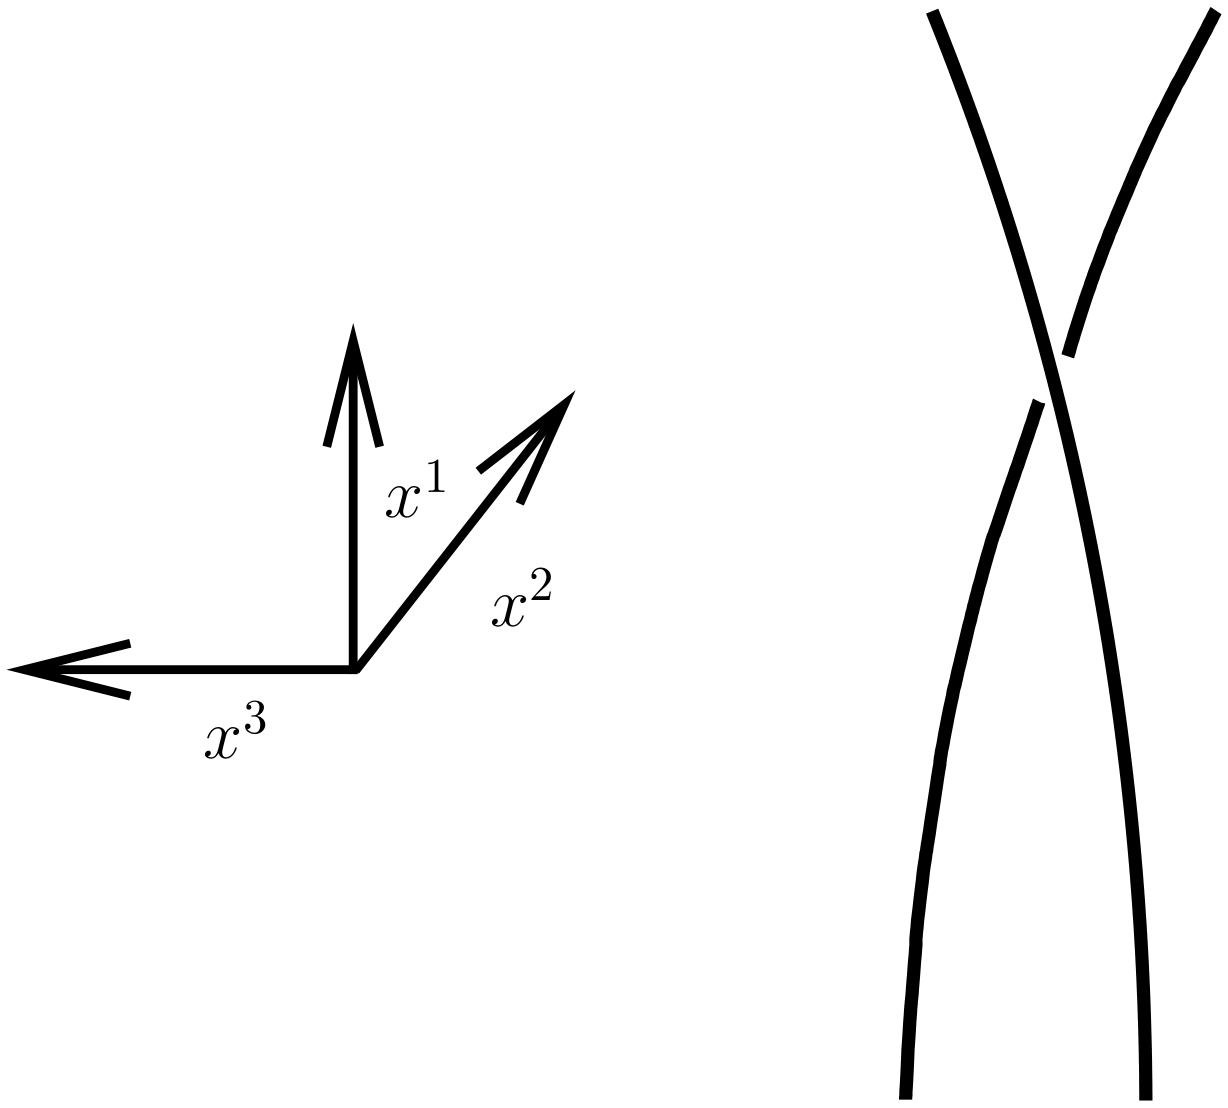
\includegraphics[width=3.5in]{figs/Fig18.png}
 \end{center}
\caption{\small 导致 Morse 理论流的过程的三维图像。图中只画了两股。$x^1$ 方向竖直向上，$x^2$ 方向指向纸内。我们沿负 $x^2$ 轴方向观察此图。坐标 $x^2$ 与 $x^3$ 组合成复变量 $z=x^2+ix^3$。对于复对称性破缺方向的某一特定选择，非平凡 Morse 理论流只能发生在这样的 $x^1$ 值处：两股在该处具有相同的 $x^3$ 值，从而在 $x^1-x^3$ 平面中投影到同一点。用纽结理论的语言来说，我们通过把纽结或链环投影到 $x^1-x^3$ 平面而得到二维图像。在这一投影中会出现交叉点，而非平凡 Morse 流可能发生的位置正是这些交叉点。（原稿第 76 页）\label{crossing}}
\end{figure}

三维图像使问题变得清楚（图~\ref{crossing}）。当两股沿 $x^2$ 方向对齐时，就可能出现 Morse 流。Morse 流发生的时间尺度比绝热演化快得多，因此在绝热图像中它实质上是瞬时的。该流涉及一个 Bethe 根朝正 $x^2$ 方向移动。这种流只能发生在荷相反的股之间，并且只允许正荷朝正 $x^2$ 方向移动。

一般地，给定任意纽结，我们可以有用地把它投影到 $x^1-x^3$ 平面，并从负 $x^2$ 方向观察。我们假定纽结在 $\R^3$ 中的嵌入足够一般，使其切矢量在 $x^1-x^3$ 平面上的投影处处非零；并且纽结到该平面的投影只有简单交叉；最后还假定函数 $x^1$ 沿纽结只有简单的极大值与极小值。一个简单的纽结投影例子见图~\ref{winding}。在这样的纽结投影中，低能阿贝尔描述在离开交叉点处有效，因此在离开交叉点以及局域极大、极小值处（后者我们将在第~\ref{creand}~节讨论），每一股都可以用其磁荷 1 或 $-1$ 来标记。交叉点处荷不变，除非正荷的一股从负荷的一股上方经过，此时可能发生荷交换过程（在 Morse 理论中对应于非平凡梯度流）。

\begin{figure}
 \begin{center}
     % >>> 原文图 19（原稿第 77 页）
  
\includegraphics[width=1.2in]{figs/Fig19.png}
 \end{center}
\caption{\small 纽结投影的一个简单例子，其中只有简单交叉以及高度函数的简单极大值与极小值。此图还说明：有向纽结到平面的投影使人们能够定义一个整数不变量 $p=(1/2\pi)\oint\d s \,\d\theta/\d s$，它等于绕纽结一周时纽结切矢量所定义的角 $\theta$ 的总变化量。对图中所示的例子，$p=2$。$p$ 是纽结投影的唯一可以写成沿纽结的局域积分的不变量。它依赖于投影的选取，并非纽结 {\it per se} 的不变量。（原稿第 77 页）}
 \label{winding}
\end{figure}

\begin{figure}
 \begin{center}
     % >>> 原文图 20（原稿第 77 页）
  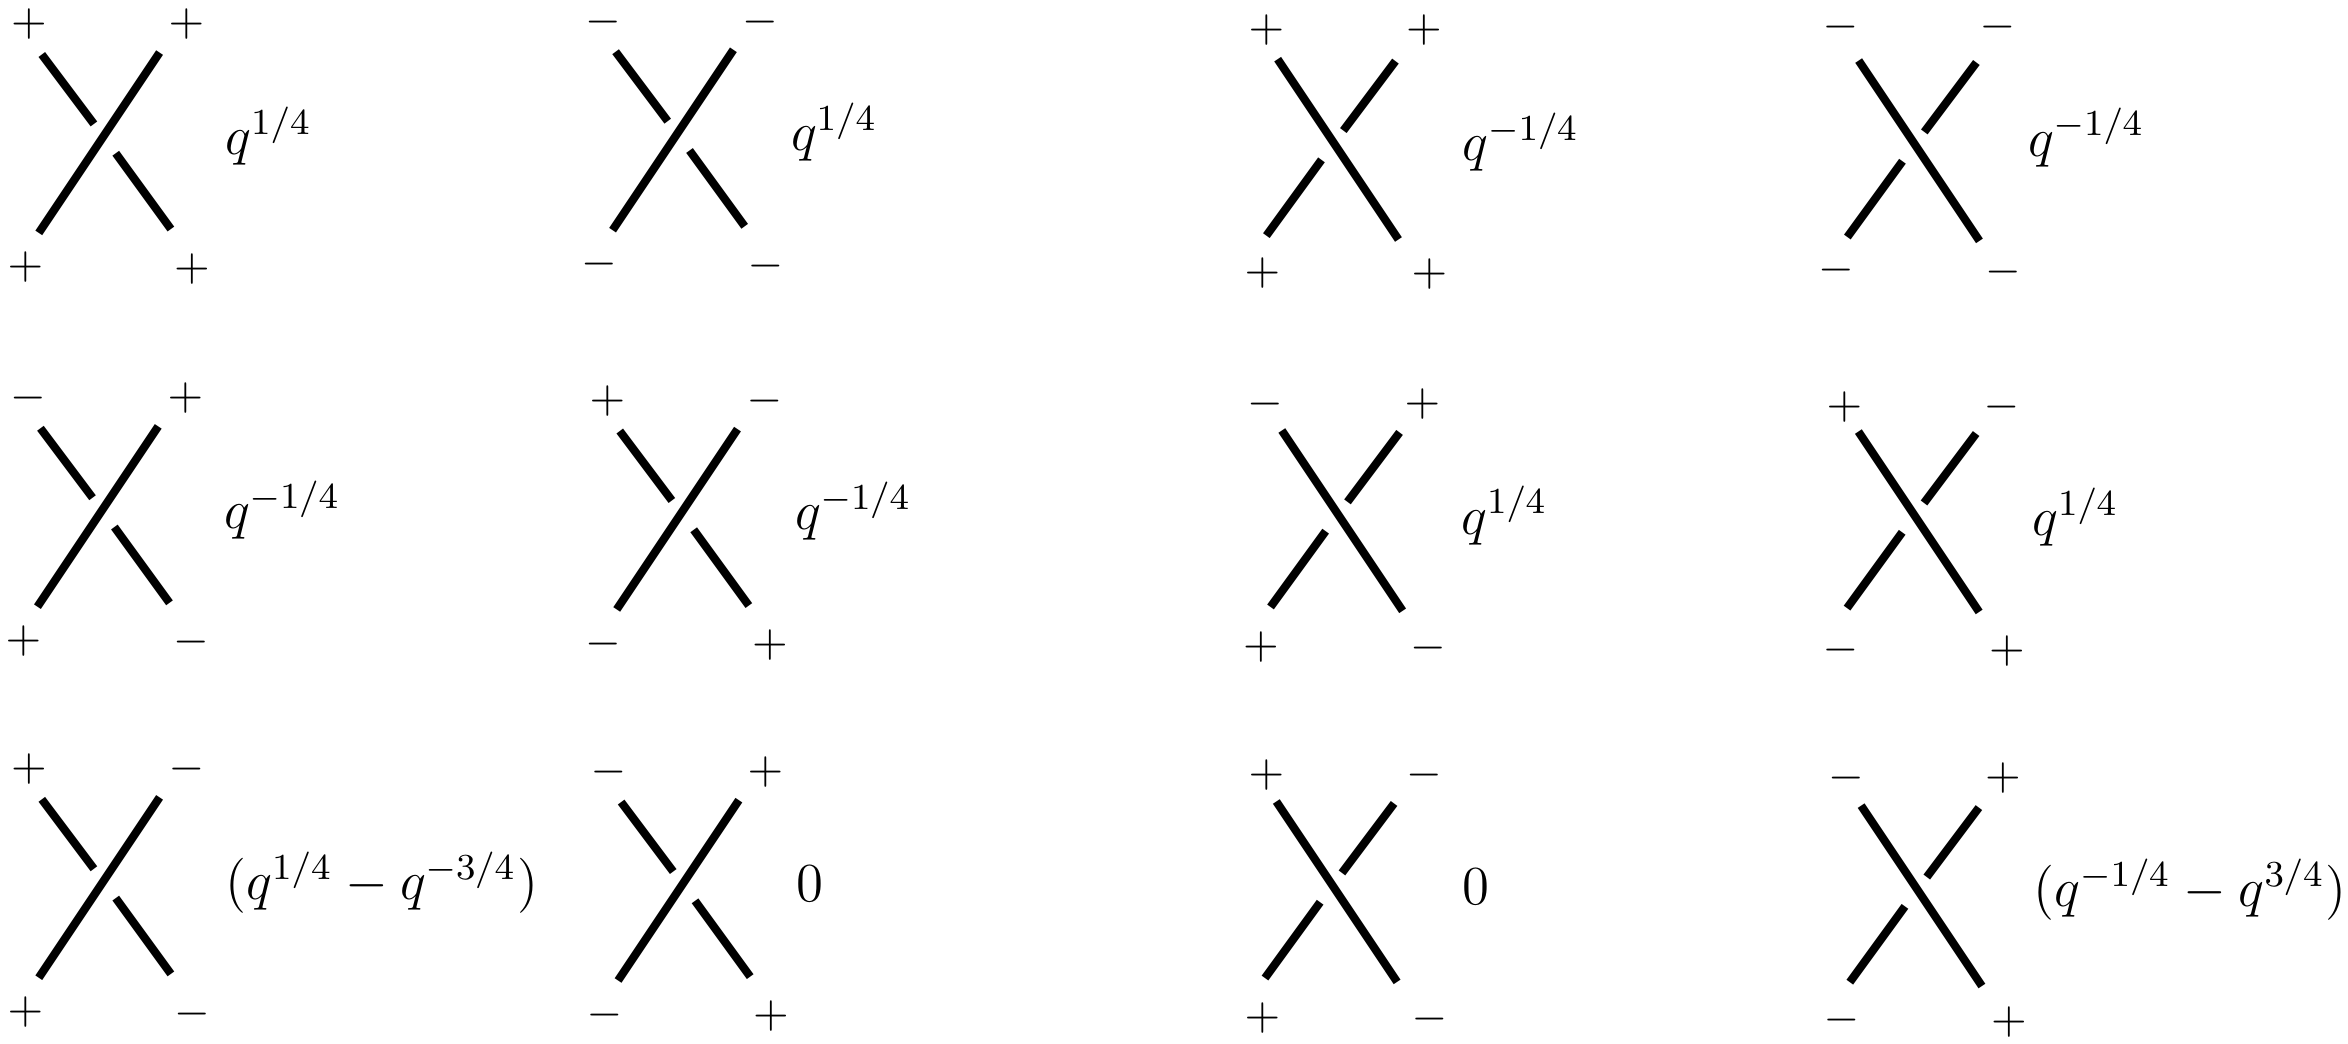
\includegraphics[width=6in]{figs/Fig20.png}
 \end{center}
\caption{\small 顶点模型为两股的每个交叉赋予图中所示的因子。标记各股的 $+$ 与 $-$ 号表示磁荷 $+1$ 或 $-1$ 的向上流动；若把图上下翻转，则只要交换所有 $+$ 与 $-$ 标记，权重保持不变。荷可以在股之间交换，但只有当正荷从底部流入、位于负荷上方时才会发生。若把图左右反射，同时把 $q$ 换成 $q^{-1}$，权重保持不变；这反映了 Chern-Simons 理论在取向反转下的行为。（原稿第 77 页）\label{vertexweights}}
\end{figure}
我们此前的计算为每个可能的交叉赋予一个权重。若交叉处荷不变，这些权重就是 $q^{\pm 1/4}$。当荷发生跳跃时，权重为 $q^{\pm 1/4} - q^{\mp 3/4}$。这些权重总结于图~\ref{vertexweights}。我们已经得到一个已知的顶点模型表示，它表示与 Jones 多项式相伴的辫群表示。
例如可参见文献~\cite{Kauffman} 第 $125$ 页上的 $R$-矩阵（其中 $A$ 就是我们的 $q^{1/4}$），或参见文献~\cite{KauffmanTwo}，特别是第 1777-8 页，或文献~\cite{Vertex} 的图 10。

% [Tutor Note: 易错点] 荷跳跃时的权重 $q^{\pm1/4}-q^{\mp3/4}$ 是两个指数之差，注意后一项是 $3/4$ 而不是 $1/4$；它来自“多出一个 $w$ 的针”与“少一个 $w$ 的针”之间的相对 $q$ 幂次（$q^{1/4}\cdot q^{-1}=q^{-3/4}$）。若把它误写成 $q^{\pm1/4}-q^{\mp1/4}$，顶点模型的 Reidemeister 不变性检验就会失败，这是核对顶点模型权重时最快的自检方式。

\subsubsection{股的产生与湮灭}\label{creand}

为了重现纽结不变量，我们需要理解绝热近似失效的位置，即两股被产生或湮灭的位置。尽管绝热近似在这类点附近失效，低能阿贝尔描述仍然有效。作为一个直接推论，阿贝尔理论中的荷守恒清楚地表明：只能产生或湮灭荷相反的一对股。


从微观理论中的线算符到低能有效描述中的线算符的映射，类似于局域算符的相应映射，但有一点小曲折：系数不是 $c$-数，而是必须沿线输运的量子力学矢量空间。在目前的情形下，这些矢量空间是一维的（在 $U(1)$ 理论中，'t Hooft 算符除其荷之外没有其他结构），但我们仍可从平行输运中得到一个整体因子。这个因子必须沿圈局域地写出，并且必须与拓扑不变性相容。对于没有任何附加结构的纽结，不存在可以写成沿纽结的局域积分的拓扑不变量；但一旦给定纽结到平面（在我们的情形中是 $x^1-x^3$ 平面）的投影，就恰好有一个这样的不变量，即纽结切矢量的总绕数（图~\ref{winding}）。它可以写成 $(1/2\pi)\oint \d s\,\d \theta/\d s$，其中纽结由变量 $s$ 参数化，$\theta$ 是纽结切矢量在 $x^1-x^3$ 平面中的角方向。为定义该不变量的符号，需要纽结的一个取向；在我们的情形中，这来自磁荷的流动方向。当微观 $SU(2)$ 理论在长距离下近似为有效 $U(1)$ 理论时，'t Hooft 算符的有效作用量可能获得一项 $-i\eta\oint \d s \,\d \theta/\d s$，其系数 $\eta$ 是普适的。若纽结的切方向转过角度 $\Delta\theta$，这将贡献一个因子
\begin{equation}
\exp (i\eta \Delta \theta)
\end{equation}
在一对股的产生或湮灭中，切角的变化为 $\Delta\theta=\pi$ 或 $-\pi$，取决于正荷向左还是向右弯折。这一效应会给每个产生或湮灭事件赋予一个普适因子 $\exp(\pm i\pi \eta)$，取决于荷的流动方向。

在相差一个符号的意义下，导致纽结不变量成立的 $\eta$ 的选取是唯一的，即 $\exp(i\pi\eta)=\mp iq^{1/4}$。符号的选择无关紧要，因为每个纽结的产生与湮灭事件数都是偶数；我们将取 $\exp(i\pi\eta)=-iq^{1/4}$。取此 $\eta$ 值时产生与湮灭事件的权重见图~\ref{creation}。$\eta$ 的值或许可以通过研究四维规范场论 BPS 方程在阿贝尔极限附近的行为来直接计算。$q^{1/4}$ 因子应表达在 $SO(3)$ 理论中微观计算的瞬子数与在低能 $U(1)$ 理论中计算的瞬子数之差。$\mp i$ 因子则应涉及 $SO(3)$ 与 $U(1)$ 的费米子行列式之间的比较。整体而言，给定经典解对 Jones 多项式的贡献正比于费米子行列式的符号——这是一个微妙的量，可能接收到微观 $SO(3)$ 理论中带电模的贡献；要把这个符号写成局域因子的乘积，看来必须使用 $i^{\pm 1}$ 这样的因子，而整体符号取决于人们如何把行列式线丛平凡化。

% [Tutor Note: 原文存疑] 本段先写 $\exp(i\pi\eta)=\mp iq^{1/4}$，而两段之后由 (\ref{golf}) 的系数比推出的是 $\exp(i\pi\eta)=\mp i q^{-1/4}$；两处的 $q$ 幂次相反。按后文的推导（比值 $-q^{-1/2}=\exp(2\pi i\eta)$）应有 $\exp(i\pi\eta)=\pm i q^{-1/4}$，故本段开头的 $q^{1/4}$ 疑为笔误。按铁律公式未作改动，请以推导为准。

实际上，$\eta$ 的值可以通过结合阿贝尔描述中可得的信息与共形块描述中可得的信息来推出。当一对股被产生或湮灭时，我们预期它们融合为恒等场。这意味着位于 $z_1$ 与 $z_2$（比如）处的两条邻近的股伴随一个 Bethe 根 $w$，而该 Bethe 根的积分链是连接 $z_1$ 与 $z_2$ 的针 $\CC_{12}$。另一方面，在第~\ref{twop}~节中我们还定义了积分链 $\tilde \CC_1$ 与 $\tilde \CC_2$，其性质是 $z_1$ 处与 $z_2$ 处的股具有确定的磁荷。（例如，在 $\tilde \CC_1$ 中 Bethe 根伴随 $z_1$，因此两股的荷分别为 1 与 $-1$。我们按 $x^3=\mathrm{Im}\,z$ 递减的次序排列 $z_1$ 与 $z_2$。）这些链之间的关系为
\begin{equation}\label{golf}\CC_{12}=\CC_1-\CC_2=q^{-1/4}\tilde\CC_1-q^{1/4}\tilde \CC_2.
\end{equation}
产生一对荷 $(1,-1)$ 的振幅与产生一对荷 $(-1,1)$ 的振幅之比，等于 (\ref{golf}) 右端系数之比，即 $-q^{-1/2}$。另一方面，在阿贝尔描述中该比值为 $\exp(2\pi i\eta)$。于是 $\exp(i\pi\eta)=\mp i q^{-1/4}$，如图~\ref{creation} 所示。



\begin{figure}
 \begin{center}
     % >>> 原文图 21（原稿第 79 页）
  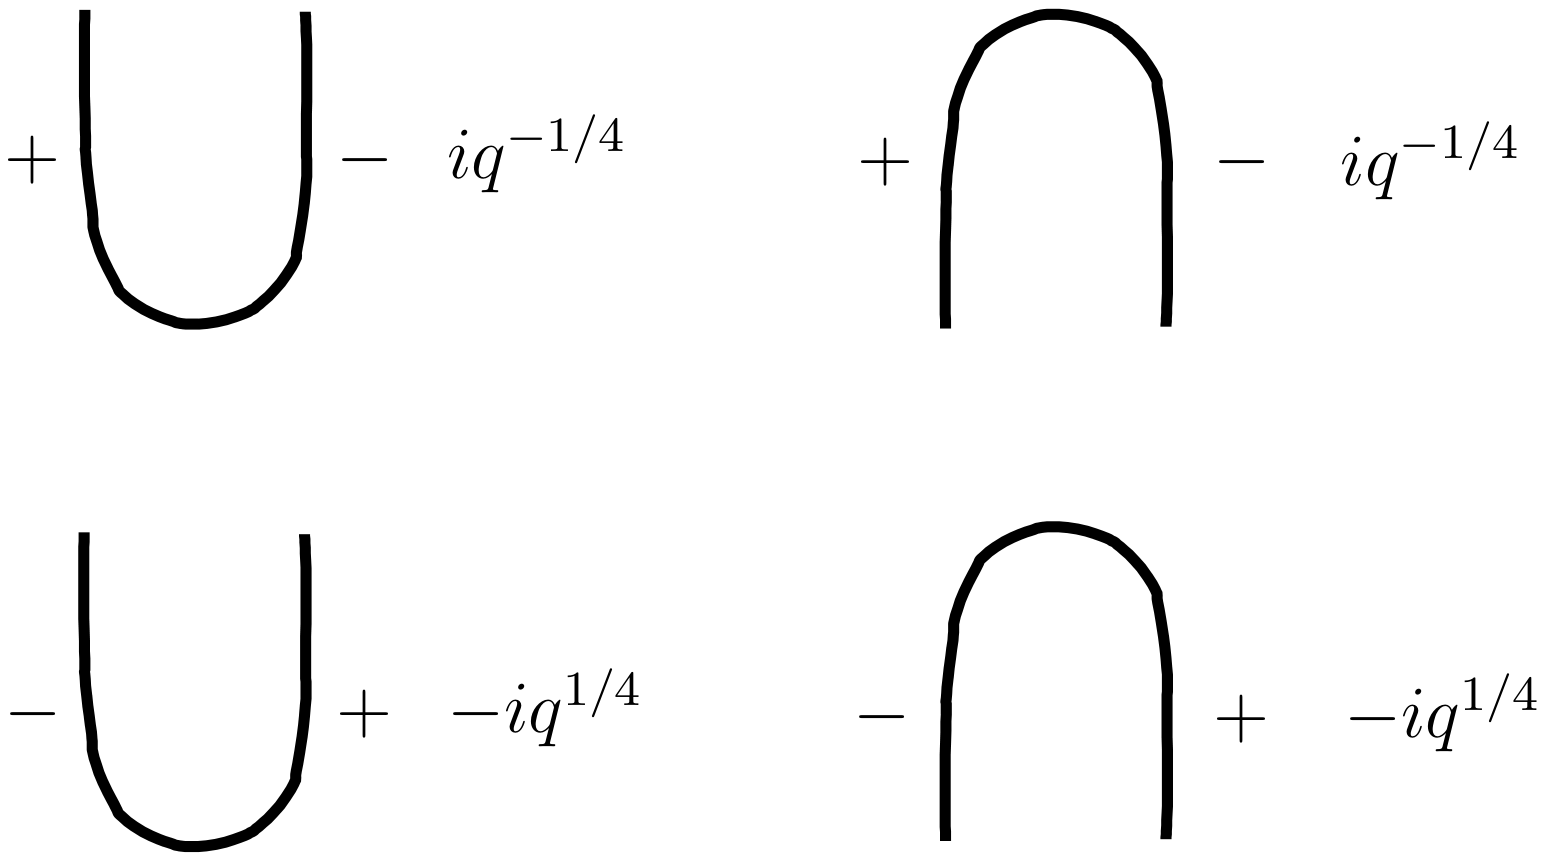
\includegraphics[width=4in]{figs/Fig21.png}
 \end{center}
\caption{\small 一对股产生或湮灭时顶点模型的权重。如图~\ref{vertexweights} 那样，若交换 $+$ 与 $-$ 标记，则权重在把图上下翻转时不变；若把 $q$ 换成 $q^{-1}$，则权重在左右反射下不变。（原稿第 79 页）\label{creation}}
\end{figure}

我们已经得到了本质上标准的、用于计算 Jones 多项式的顶点模型算法：给定一个纽结或链环，选取它到 $x^1- x^3$ 平面的投影，使得投影中只有简单交叉，且函数 $x^1$ 只有简单的极大值与极小值。把链环分成由极大值、极小值与交叉点分隔的线段。用 $\pm$ 标记各线段，并对所有标记求和，每个标记以交叉点、极大值与极小值处局域权重的乘积加权。
稍后我们会给出一些简单的例子。
   % §6  积分链表示的编织（中段）
\subsubsection{一些例子与若干拓扑细节}\label{details}

\begin{figure}
 \begin{center}
     % >>> 原文图 22（原稿第 80 页）
  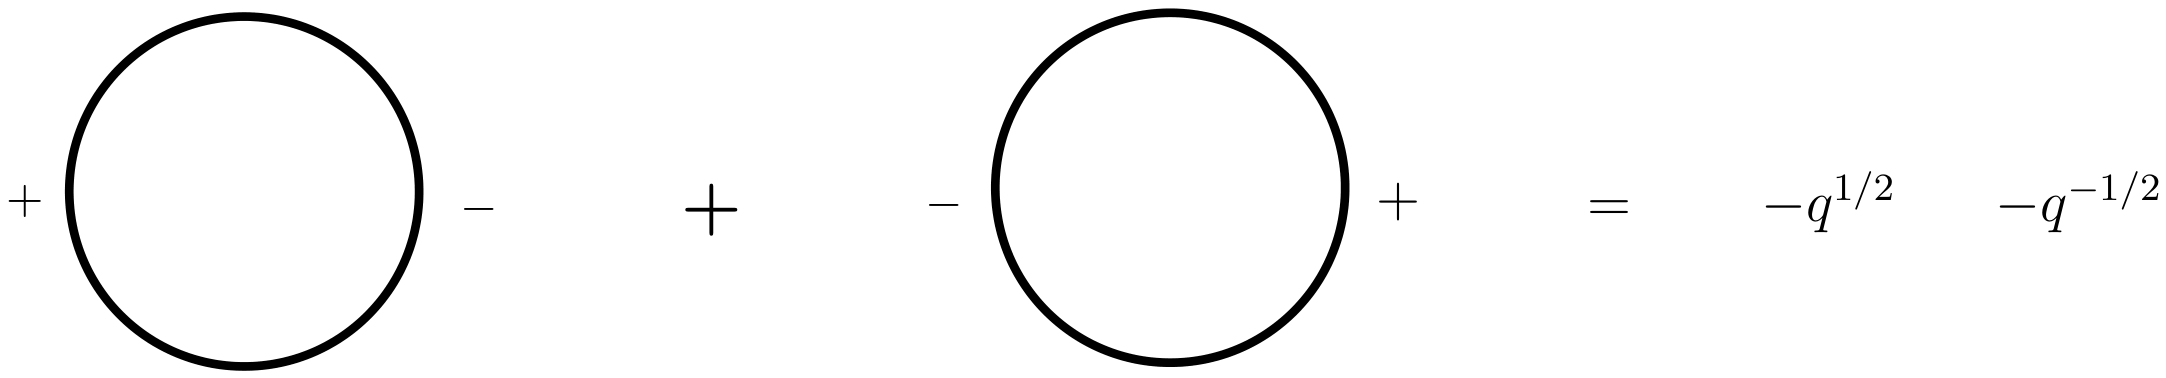
\includegraphics[width=5.5in]{figs/Fig22.png}
 \end{center}
\caption{\small 以最显然的方式投影到平面上的一个平凡纽结。图中没有交叉，但有一个产生事件与一个湮灭事件。在顶点模型中，平凡纽结的不变量通过对纽结两侧（即交叉、产生与湮灭事件之间的各线段）用荷 $+$ 或 $-$ 标记的所有方式进行求和来计算。每个标记以相应局域因子的乘积加权。在当前的例子中，只有图中所示的两种选择给出非零贡献，于是立刻得到结果 $-q^{1/2}-q^{-1/2}$。（原稿第 80 页）}
 \label{unknot}
\end{figure}
作为使用顶点模型的最简单例子，我们来计算一个以显然方式投影到平面上的平凡纽结的期望值（图~\ref{unknot}）。对图形的两种可能标记求和，我们得到结果 $-q^{1/2}-q^{-1/2}$。

\begin{figure}
 \begin{center}
     % >>> 原文图 23（原稿第 81 页）
  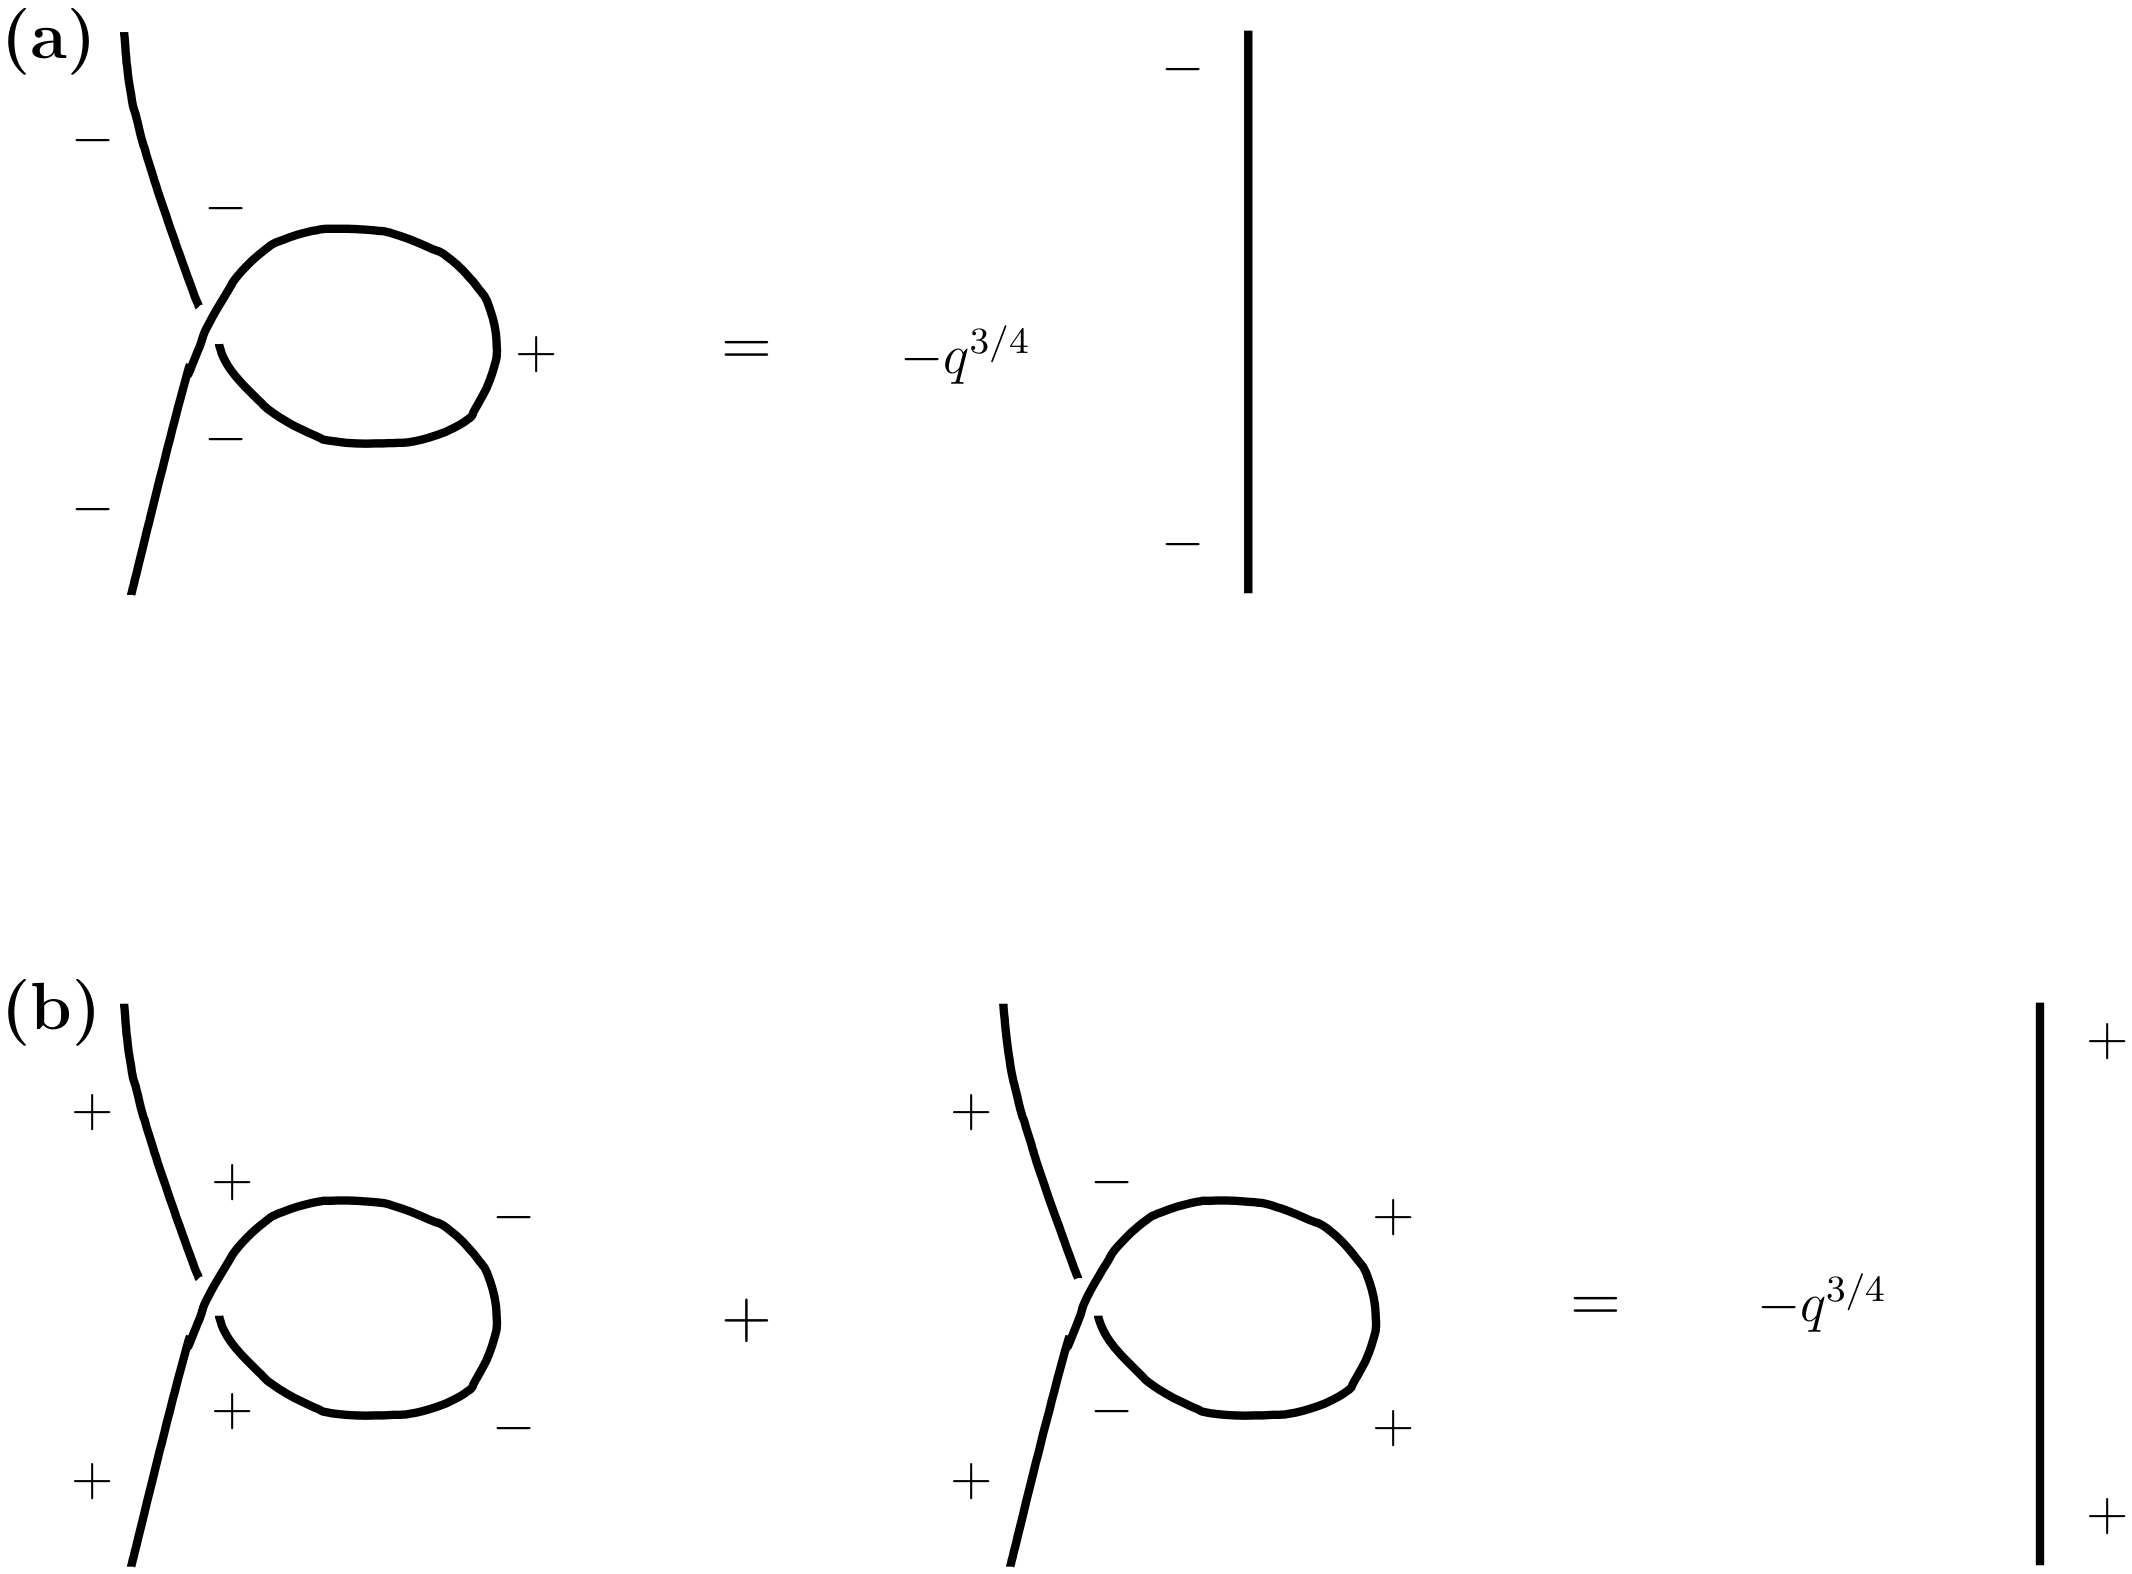
\includegraphics[width=5.5in]{figs/Fig23.png}
 \end{center}
\caption{\small  
 \label{twist}  用顶点模型比较单股到 $x^1-x^3$ 平面的两种不同投影——带扭结（左）与不带扭结（右）。无论该股所带荷的符号如何，扭结都引入一个因子 $-q^{3/4}$。对该股所带荷的两个可能取值，计算相当不同；对荷 $-1$，如 (a) 所示，顶点模型求和只有一个非零贡献，对应于图中标出的标记；但对荷 $+1$，有两种可能的贡献，如 (b) 所示，它们相加得到同一结果。在 (b) 中，第二个贡献涉及一个荷交换过程：上下两股在交叉处交换荷。类似地，若把上穿换成下穿（或把整幅图换成镜像），则相反会给出因子 $-q^{-3/4}$，读者可自行验证。（原稿第 81 页）}
\end{figure}

作为一个稍不那么平凡的例子，我们考虑图~\ref{twist} 所示的单股到 $x^1-x^3$ 平面的两种投影。无论在 (a) 还是 (b) 中，左右两侧所示的纽结投影都可以彼此形变，因此人们也许预期它们等价。
但在当前语境下，事实并非如此。(a) 相对于 (b) 的扭结引入一个因子 $-q^{3/4}$，可以利用顶点模型的权重把它算出来。实际做一遍是有启发性的；无论该股的磁荷是 $+1$ 还是 $ -1$，都出现同一个因子 $-q^{3/4}$，但两种情形下计算的细节相当不同。

% [Tutor Note: 易错点] 这里的关键是“同一个因子、不同的计算”：荷为 $-1$ 时只有一条标记路径非零，因子直接读出；荷为 $+1$ 时有两条路径，其中一条经过荷交换过程，两条贡献相加后才给出同一个 $-q^{3/4}$。若只算其中一条就会得到与荷有关的因子，从而误以为扭结因子不普适。核对时可验证两条贡献的比值恰为 $-q^{-1}$（见 (\ref{twof}) 的相对因子）。

由于因子 $-q^{3/4}$ 不依赖于某一股所带的磁荷，它是普适的：在任意纽结或链环的任意一股上添加图中所示类型的一个扭结，都会使相应的不变量乘以 $-q^{3/4}$。手性相反的类似扭结则使不变量乘以 $-q^{-3/4}$，理由类似。这个因子意味着：量子场论赋予纽结（或链环）的不变量依赖于“标架”（framing）的选取。标架纽结是把纽结稍加增厚成一条带子。人们追踪带子如何扭结，而（在当前语境下）添加一个扭结会使不变量乘以因子 $-q^{3/4}$。以平面投影给出的纽结自带一个自然的标架，它由沿垂直于平面的竖直方向作轻微增厚给出。稍加思考（或用一条纸条做实验）即可看出：尽管在忽略标架时图~\ref{twist}(a) 或 (b) 左右两图在拓扑上等价，它们确实相差一个单位的标架。

% [Tutor Note: 物理图像] 标架（framing）在此不是可有可无的装饰：把纽结增厚成带子后，“扭一下”是拓扑上非平凡的形变，于是不变量只能定义在标架纽结上。本文的顶点模型计算隐含地固定了由“竖直增厚”给出的标架，因此图~\ref{twist} 左右两图虽然作为无标架纽结等价，却相差一个标架单位、恰好给出 $-q^{3/4}$。这也解释了为什么 Jones 多项式需要标架（或等价地，需要把 $q$ 的幂次按 writhe 修正）。

在与二维共形场论相伴的三维纽结不变量的语境下，二维的共形初级场对应于三维中的线算符。若共形初级场的维数为 $h$，那么标架改变一个单位时，相应的线算符要乘以 $\exp(2\pi i h)$。因子 $-q^{3/4}$ 确实就是 $\exp(2\pi i h)$，其中退化 Virasoro 初级场 $V_{-k/2b}$ 的共形维数为
\begin{equation}\label{maxi} h_V(k) =-\frac{k}{2}-\frac{k(k+2)}{4b^2},\end{equation}
此外 $q=\exp(-2\pi i/b^2)$，而我们描述的顶点权重是针对最小荷情形 $k=1$ 的。

% [Tutor Note: 易错点] 请核对这个恒等式：把 $k=1$ 代入 (\ref{maxi}) 得 $h_V(1)=-\frac12-\frac{3}{4b^2}$，故 $\exp(2\pi i h_V(1))=e^{-\pi i}\cdot e^{-3\pi i/(2b^2)}=-q^{3/4}$（其中用到 $q^{3/4}=e^{-3\pi i/(2b^2)}$）。负号来自 $e^{-\pi i}$，即 $k/2$ 这一项；若漏掉它，就会得到 $+q^{3/4}$，与顶点模型的计算不符。这也正是下一段 Chern-Simons 归一化差异的来源。

至此出现一个重要细节。我们所描述的顶点权重适用于 Jones 多项式的某种自然归一化，这种归一化在文献中（例如文献~\cite{Kauffman} 中）被使用。然而，在 $SU(2)$ Chern-Simons 理论中出现的是略有不同的归一化。在 Chern-Simons 理论中，由 $SU(2)$ 二维表示标记的平凡纽结的期望值为 $q^{1/2}+q^{-1/2}$，其符号与我们用顶点权重在图~\ref{unknot} 中得到的相反。（这个符号在 Chern-Simons 理论中容易核对。由于在 $SU(2)$ Chern-Simons 理论中 $q=\exp(2\pi i/(\k^\vee+2))$，其中 $\k^\vee$ 是能级，弱耦合极限 $\k^\vee\to\infty$ 对应于 $q=1$；当 $q=1$ 时，任一表示中 Wilson 圈的期望值就是该表示的维数，对二维表示而言为 $+2$。）类似地，与 $SU(2)$ 自旋 $j=k/2$ 的表示相关的初级场的维数为
\begin{equation}h_{\mathrm{CS}} (k)=\frac{k(k+2)}{4(\k^\vee+2)},\end{equation}
于是在标架改变一个单位时获得的因子为 $\exp(2\pi ih_{\mathrm{CS}})=q^{3/4}$，不带图~\ref{twist} 中出现的负号。显然，符号的差异反映了如下事实：$h_V(k)-h_{\mathrm{CS}}(k)=-k/2$，它与 $b$ 和 $\k^\vee$ 无关。

与 Chern-Simons 理论的比较对本论文未必构成问题，因为我们只是从四维规范场论方程 (\ref{bpseqns}) 出发。然而，人们希望知道，在文献~\cite{fiveknots} 所给出的 Chern-Simons 理论 Wilson 算符与边界奇异磁单极子之间的对偶的语境下，这些符号的最佳解释是什么。我们相信，解释或许是：Chern-Simons 理论中自旋 $k/2$ 的 Wilson 算符，其对偶实际上是边界上的一个 't Hooft 算符，它带有角动量 $k/2$，并在 $k$ 为奇数时是费米性的。（对于定义在四维流形边界上的 't Hooft 算符，相关的旋转群是 $SO(2)$，或更确切地说是其双重覆盖 $\mathrm{Spin}(2)$；该群是阿贝尔的，具有一维表示，以角动量 $k/2$ 标记。）
奇数 $k$ 的费米统计会为每个交叉给出一个负号（相对于图~\ref{vertexweights} 所呈现的内容），并为每个闭合圈给出一个负号；把这些符号计入后，由 Virasoro 退化场编织得到的结果就与在 Chern-Simons 理论中编织得到的结果一致。

最后，把图~\ref{twist} 中的计算与规范群简单取为 $G=U(1)$（而非 $SO(3)$）时的相应计算作比较，是有启发性的。会有两处差别。第一，图~\ref{creation} 中与一对股的产生和湮灭相伴的因子将简单地等于 1。（那些因子完全来自在低能下约化为有效阿贝尔描述时对 $SO(3)$ 理论大质量自由度的积分掉。）第二，对 $G=U(1)$，荷交换过程不存在（因为没有光滑磁单极子），因此图~\ref{twist}(b) 中的第二个贡献将不存在。回顾图~\ref{vertexweights} 可见，对 $G=U(1)$，图~\ref{twist}(a) 或 (b) 的计算给出简单的因子 $q^{1/4}$，而不是 $-q^{3/4}$。
有两点评论：\begin{itemize}\item 对 $G=U(1)$，图~\ref{twist} 的负号不存在（类似地，图~\ref{unknot} 中的负号也不存在）。\item 在 Chern-Simons 理论中，$q$ 的幂次是 $G^\vee$ 相应表示的二次 Casimir 不变量。最高权为 $j$ 的表示的二次 Casimir，对 $G^\vee=U(1)$ 为 $j^2$，对 $G^\vee=SU(2)$ 为 $j(j+1)$。对 $j=1/2$，这在阿贝尔与非阿贝尔情形下分别给出 $q^{1/4}$ 与 $q^{3/4}$。\end{itemize}

% [Tutor Note: 数学工具] 二次 Casimir 的比较给出了一个方便的记账规则：$q$ 的幂次 $=$ 表示的最高权 $j$ 的函数，$U(1)$ 用 $j^2$、$SU(2)$ 用 $j(j+1)$。对 $j=1/2$ 分别得 $1/4$ 与 $3/4$，正好解释图上看到的 $q^{1/4}$ 与 $q^{3/4}$；这也说明为什么非阿贝尔情形会出现“多出来”的 $j$ 项（即 $j(j+1)-j^2=j$）。核对任何顶点权重时，先数出表示的最高权，再套此规则，可迅速判断指数是否算对。

\subsubsection{梯度流与弦}\label{morsestrings}

\begin{figure}
 \begin{center}
     % >>> 原文图 24（原稿第 83 页）
  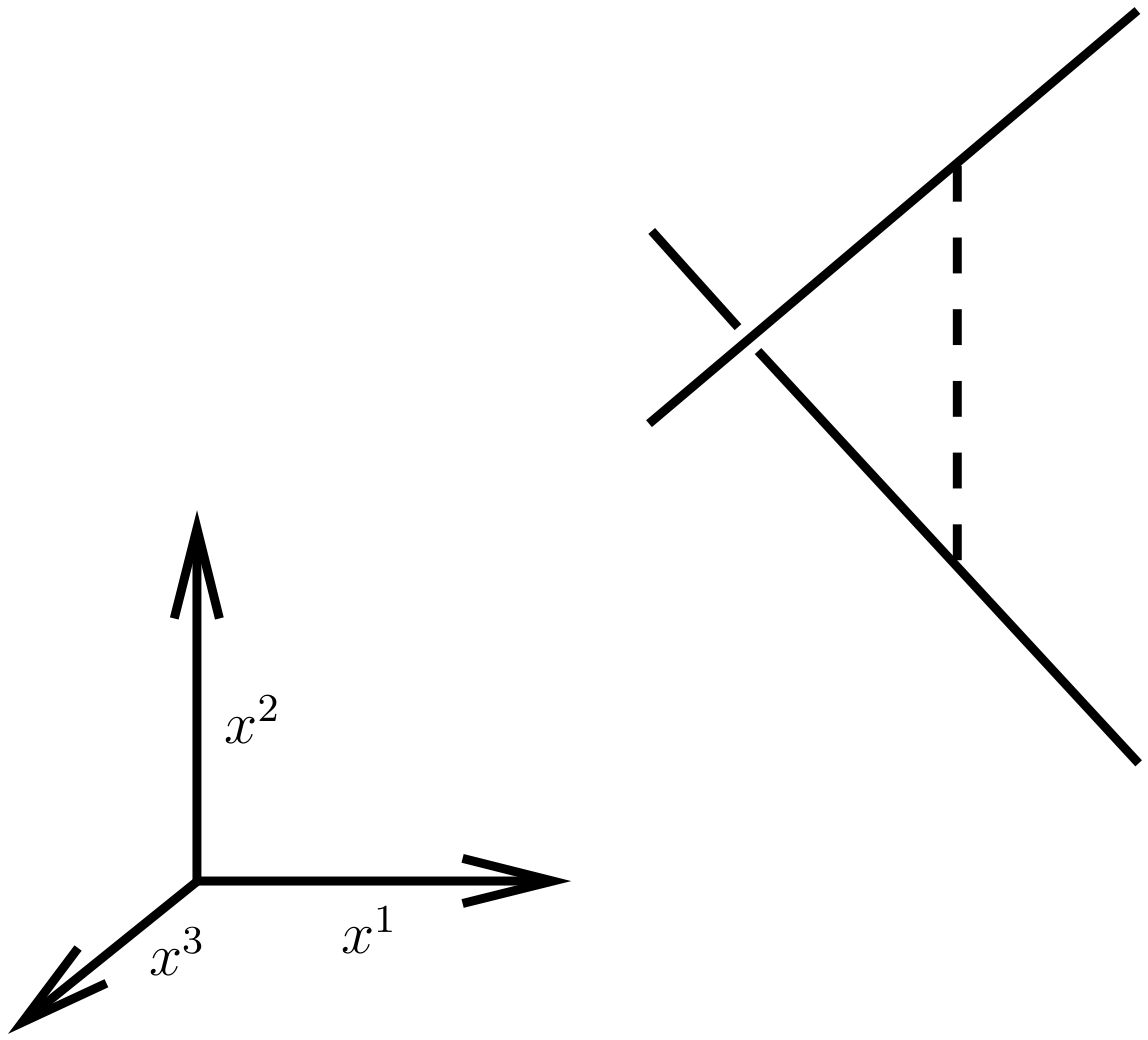
\includegraphics[width=3in]{figs/Fig24.png}
 \end{center}
\caption{\small 为使荷交换过程更清楚可见，我们相对于图~\ref{crossing} 交换了坐标轴。$x^2$ 轴现在竖直，而 $x^1$ 水平。荷交换发生在这样的 $x^1$ 值处：两股在该处仅在 $x^2$ 的取值上不同；因此按本图的坐标轴取向，荷交换涉及沿竖直方向的荷流动，由虚线表示。我们把它解释为 BPS 孤子的传播。该孤子沿对称性破缺轴传播，因此它由仅含实对称性破缺的解来描述——实际上就是由式 (\ref{onl}) 的裸 Miura oper 描述，不含 't Hooft 算符且只有一个 Bethe 根。（原稿第 83 页）\label{soliton}}
\end{figure}
我们可以对适当荷的股交叉时出现的梯度流给出更具体的物理解释。磁荷从一股传播到另一股，可以用一个磁单极子在这两股之间的运动来描述。
若旋转坐标并把 $x^2$ 方向视为“时间”，我们就应当能把相关对象看成仅存在实对称性破缺时的不含时解。

事实上，我们已经精确描述过所需的解：它对应于式 (\ref{onl}) 所描述的、只有一个 Bethe 根且没有奇异磁单极子的裸 Miura oper。因此我们把荷交换过程形象化为一个物体沿 $x^2$ 方向的传播，如图~\ref{soliton} 所示。这一图像过于简化，因为它忽略了垂直于包含纽结的边界 $\R^3$ 的第四维的存在。展示 $y$ 方向作用的另一种图像见图~\ref{bending}。沿 $x^2$ 方向传播时，孤子会停在由裸 Miura oper 的解所给出的某个 $y$ 值处。（如何计算这个值，在第~\ref{supermon}~节有最完整的说明。）当然，这一描述只有在孤子在 $x^2$ 方向传播得足够远、从而有“时间”达到 $y$ 的平衡值时才成立。因此它只在各股彼此充分远离、或对称性破缺足够强时才成立。
\begin{figure}
 \begin{center}
     % >>> 原文图 25（原稿第 84 页）
  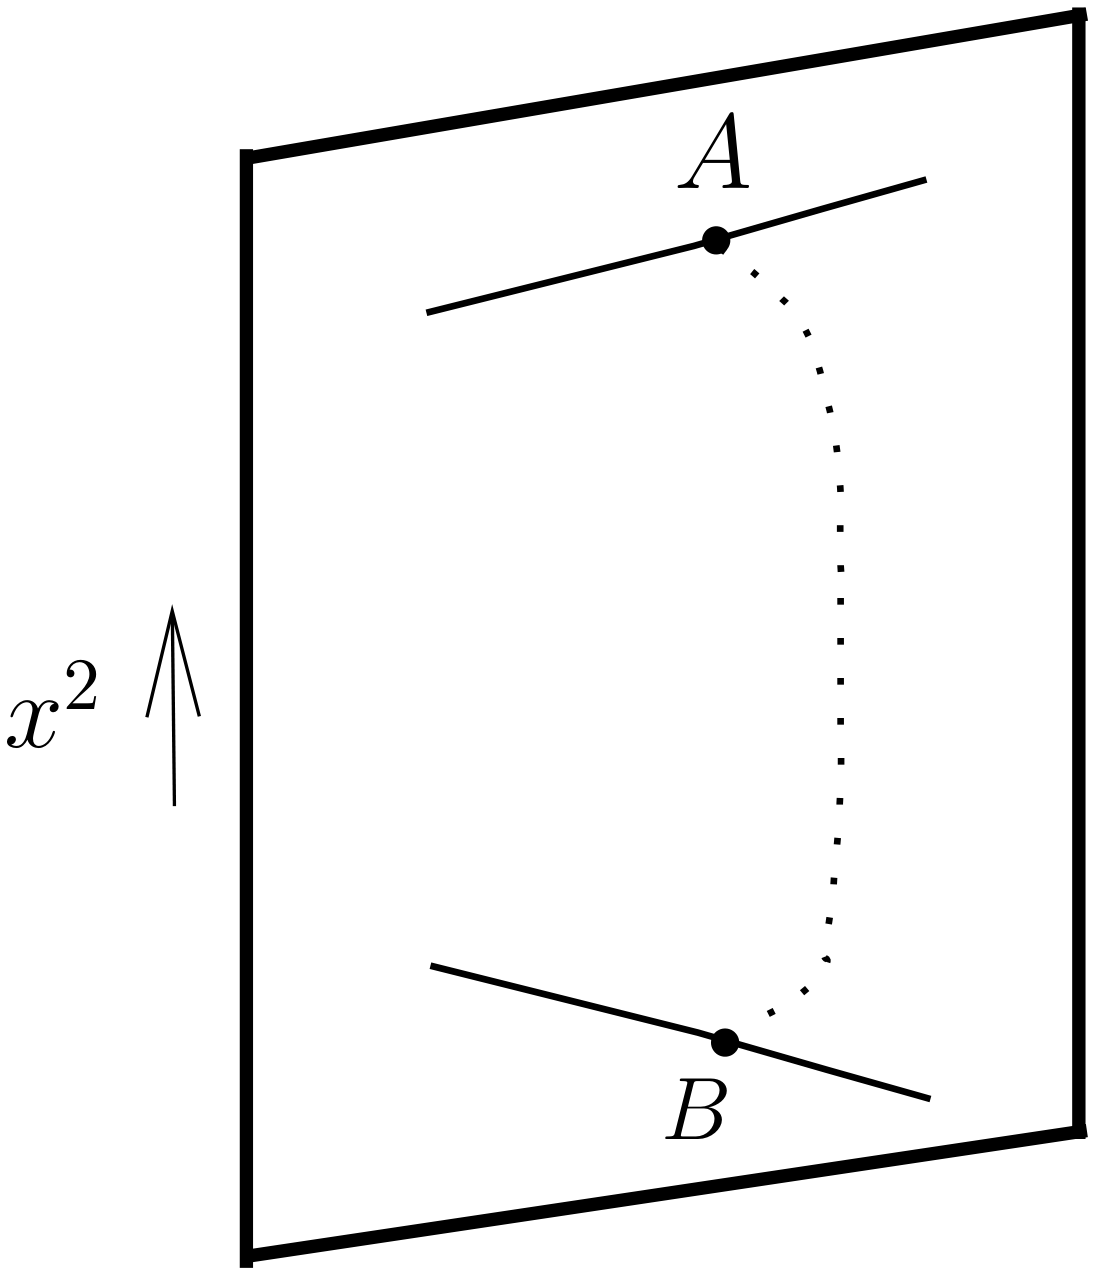
\includegraphics[width=3in]{figs/Fig25.png}
 \end{center}
\caption{\small 图~\ref{soliton} 所述荷交换过程的另一种视图，用以展示 $y$ 方向的作用（此处该方向被画成垂直于包含两股的平面）。在 $x^2$ 方向上相距很远的两个边界点 $A$ 与 $B$ 之间传播的孤子，会弯离边界，以达到对应于裸 Miura oper 解的 $y$ 值。（原稿第 84 页）\label{bending}}
\end{figure}

我们已经对强对称性破缺下四维 BPS 方程的解获得了直观图像：它们描述在奇异磁单极子股之间拉展开的光滑磁单极子构型。每个构型对纽结不变量的贡献是两类因子的乘积。一类来自从微观非阿贝尔理论到阿贝尔理论的映射，另一类则在阿贝尔理论中计算。第一类因子出现在成对的股被产生或湮灭之处、以及光滑磁单极子被边界奇异磁单极子发射或吸收之处。在阿贝尔描述中，光滑磁单极子看起来也是荷为 $2$ 的奇异磁单极子，但并不附着于边界。整个构型看起来像一张磁单极子股构成的网，阿贝尔理论给它赋予一个整体的 $q$ 幂次。

\subsubsection{对偶 Chern-Simons 理论中的类比}\label{dualch}

把这一图像一路追溯到三维 Chern-Simons 理论——即在我们经由种种对偶到达本文所研究的四维描述之前——是件有趣的事。
联系这两幅图像的关键一步是 $S$-对偶；幸运的是，它在强对称性破缺下非常透明，因为它约化为阿贝尔规范场论中的电磁对偶。我们立刻得到对如下构型的求和：大质量 $W$-玻色子拉展在 Wilson 线之间，并且只携带朝正 $x^2$ 方向流动的电荷。

这提示我们在非阿贝尔 Chern-Simons 理论中寻找能产生这一效果的规范条件。它很容易被认出：可以选取一种“部分”轴规范固定，把规范场的 $A_2$ 分量约化到 Cartan 子代数中。我们把非阿贝尔规范场写成 $A=B\frak t_3+W_+\frak t_++W_-\frak t_-$，并对 $W_\pm$ 施加 $A_2=0$ 规范条件；此处不必为对角规范场 $B$ 作规范选择。带电 $W$-玻色子的作用量于是约化为
\begin{equation}
\frac{\k^\vee}{4\pi}\int \d^3x \,\,W_+ D_2 W_-,~~~   D_2=\frac{\partial}{\partial x^2}+[B_2,\,\,\cdot\,\,].
\end{equation}
传播子的方程为
\begin{equation}
D_2 G(x,y) = \frac{2\pi}{\k^\vee}\delta^3(x-y)
\end{equation}
其解为
\begin{equation}\label{dox}
\frac{2\pi}{\k^\vee} 
\exp\left(\int_{x^2}^{y^2} B_2\right)\, \delta(x^1-y^1) \delta(x^3-y^3) \theta(x^2 - y^2),
\end{equation}
后者只描述荷朝正 $x^2$ 方向的传播。
相当清楚的是，这样的部分规范固定会给出顶点模型的某个版本，尽管精确计算顶点权重可能颇为棘手。所需的计算大概与在通常轴规范下研究 Chern-Simons 理论（例如见文献~\cite{AS,Hahn}）、或在某种几乎轴规范下研究 Chern-Simons 理论（文献~\cite{Wetering}）时的计算有些类似。使用复化的轴规范来导出 Knizhnik-Zamolodchikov 方程（文献~\cite{FK}）也与此有些类似。

% [Tutor Note: 物理图像] $\theta(x^2-y^2)$ 阶跃函数是这一段的要点：它把传播严格限制在 $x^2$ 增大的方向，即“电荷只能朝正 $x^2$ 流动”。若没有它，传播子就是双向的，顶点模型里就会出现逆向的弦，从而无法得到只有一种流向的顶点权重。这与图~\ref{vertexweights} 中“正荷只能从底部流入”的规则是同一件事的场论表述。

\subsection{上至六维}
着眼未来的范畴化（categorification），把这一阿贝尔图像一路提升到六维是有用的。毕竟，在存在强对称性破缺时，六维 $(0,2)$ 理论并不那么神秘。它是自对偶二形式与重的大质量动力学 BPS 弦耦合的理论。
导致纽结不变量的六维框架，涉及乘积 $\R \times M_3 \times D$ 上的六维理论，其中 $D$ 是一个几何上半无限雪茄的 $\R^2$（见式 (\ref{cigarl})）。纽结本身由置于雪茄尖端的打结二维缺陷表示。$q$-分次来自 $D$ 的旋转对称性所导出的守恒角动量。

在不存在对称性破缺时，$D$ 上的度规是雪茄型的而非欧几里得度规，这一点对于得到良定义的缺陷态空间很重要。置于平坦六维空间中的缺陷会与体 SCFT 强耦合。另一方面，在存在对称性破缺时，红外物理是自由的，我们可以希望从动力学重弦与缺陷的束缚态中恢复态空间。此时雪茄几何将不起重要作用，$D$ 可以换成一个平坦的 $\R^2$。

现在，我们专门取 $M_3 = \R^3$，并且为简洁起见取纽结与时间无关。
不含时的动力学弦的 BPS 条件非常简单：它必须是直的，并与对称性破缺方向（我们仍取为 $x^2$ 方向）对齐。这实际上就是光滑磁单极子所满足条件的六维提升，并且投影到 $x^2$ 上时给出相同的顶点模型图像。在阿贝尔低能描述中，缺陷股有两个可能的基态，它们具有相反的二形式荷。与动力学弦的汇合允许二形式荷发生跳跃。

有趣的问题是，从六维的角度重现顶点模型的权重。这既包括由弦作为源的自对偶二形式阿贝尔理论的贡献，也包括弦的世界体积理论的贡献。我们在此不计算前者，但可以对后者给出一些洞见。

如图~\ref{vertexweights} 所总结的，对 Jones 多项式有贡献的荷交换过程的顶点模型权重为
\begin{equation}
\label{twof}q^{\pm 1/4}-q^{\mp 3/4}. \end{equation}
  在六维图像中，Jones 多项式应当来自对 BPS 态求和，权重为 $q^P(-1)^F$，其中 $P$ 是与 $D$ 的旋转相对应的守恒荷，而 $F$（可以宽松地称为费米子数）是某个 $R$-对称生成元。
我们把 (\ref{twof}) 中两项之间的相对因子 $-q^{\pm 1}$ 解释为：连接纽结中两股的 BPS 弦有两个物理态，它们在角动量上相差 1（以解释因子 $q^{\pm 1}$）、在费米子数上也相差 1（以解释负号）。
为理解这一点，我们可以把注意力集中在那两条交叉的股以及拉展在它们之间的弦上。关键在于：单股是半 BPS 的，两条不平行的股是四分之一 BPS 的，但两股交换一条 BPS 弦的构型把对称性进一步破缺到八分之一 BPS。因此该弦破缺两个超荷，从而必须有两个基态，它们被破缺超荷的作用互换。这立刻给出所需的量子数差。

% [Tutor Note: 物理图像] “破缺两个超荷 ⇒ 两个基态”的推理是本节最容易被跳过的环节：两个实超荷合成一个复的费米型升降算符 $Q$，其作用在真空上给出一个二重简并（$|0\rangle$ 与 $Q|0\rangle$），故基态数为 2；这也正是超荷多重态维数的一般规律。若破缺的超荷数为 $2n$，基态简并度应为 $2^n$，本文情形 $n=1$。这一简并度的“量子数差”（角动量差 1、费米子数差 1）正是顶点权重中 $-q^{\pm 1}$ 相对因子的来源。

因此，系统的近似基态空间可以如下描述。设 $\mathcal S$ 为顶点模型的构型集合（用 $+$ 或 $-$ 标记各股，并在标号发生跳跃的交叉处接上光滑弦）。对每条光滑弦，引入一个二维 Hilbert 空间，其量子数由上一段推出。对每个 $s\in \mathcal S$，引入一个 Hilbert 空间 $\mathcal H_s$，它定义为与各光滑弦相伴的二维因子的张量积。于是 BPS 态空间的一个近似 $\mathcal H_0$ 为 $\mathcal H_0=\oplus_{s\in\mathcal S}\mathcal H_s$。
$\mathcal H_0$ 的分次（按角动量与费米子数）受到由弦系统作为源的阿贝尔场构型的影响；例如，自对偶阿贝尔张量场可以携带角动量。

为计算 Khovanov 同调，需要求出作用在这个近似基态空间上的微分，其办法是寻找在不同态之间（在过去与未来之间）插值的瞬子构型。
含时 BPS 弦的 BPS 条件仍然相当透明。其世界面应当在复坐标 $x^0 + i x^2$ 与 $x^1 + i x^3$ 下全纯。注意：沿 $x^2$ 方向拉展的不含时弦（因而由 $x^0$ 与 $x^2$ 参数化，$x^1$ 与 $x^3$ 固定）确实具有全纯的世界体积。

因此我们预期能够由 $\R \times M_3$ 中终止于纽结的全纯曲线的数据来构造 Khovanov 同调的微分。这一途径看来对未来的发展颇有前景。
   % §6  积分链表示的编织（后段）
\section{磁单极子的有效超势}\label{supermon}

\begin{keytakeaways}
\begin{itemize}\setlength{\itemsep}{2pt}
  \item \textbf{物理图像}：$\R^2\times\R_+$ 上的光滑 BPS 磁单极子与边界上的 Nahm 极点相互作用时不存在精确解；Nahm 极点把磁单极子推向 $y\to\infty$，使其在指数精度上“几乎是解”，故其低能行为由一个有效超势支配。
  \item \textbf{数学工具}：用一对手征超场 $\sW$（$\R^2$ 中的位置）与 $\sY=\ca_1y+i\vartheta$（$y$ 位置与 $U(1)$ 集体坐标的组合）参数化单磁单极子模空间；用多项式 $K(z)=\prod_a(z-z_a)^{k_a}$ 记录边界奇异磁单极子的磁荷；通过积掉大质量场 $\sY$ 生成 $\sW$ 的有效超势。
  \item \textbf{主要结论}：有效超势为 $\W=\ca\sW+\zeta\sY+\Lambda K(\sW)\exp(-\sY)$；其临界点条件逐一复现第 2、3 节关于解存在性的定性结论；积掉 $\sY$ 后得到 Yang-Yang 函数 (\ref{longyang})，即 $\ca\sum_i\sW_i+\zeta\sum_{i,a}\log(\sW_i-z_a)-2\zeta\sum_{i<j}\log(\sW_i-\sW_j)$。
  \item \textbf{技术要点}：多个光滑磁单极子的 $\sW_i$ 重合时，$\sY_i$ 不再是好坐标，必须改用由散射矩阵定义的 $\nY_i$；两者之间的变换 (\ref{rela}) 在 $\sW_i=\sW_j$ 时发散。
\end{itemize}
\end{keytakeaways}

\subsection{结果概述}\label{outline}

从第~\ref{symbr}~节开始，我们把三维超对称方程的解解释为包含光滑 BPS 磁单极子的位形。然而，那些讨论纯粹是定性的。本节将把上述推理定量化。我们将为 $\R^2\times \R_+$ 上与 Nahm 极点以及边界上的奇异磁单极子相互作用的光滑 BPS 磁单极子构造一个有效超势。这个有效超势将直接解释第 2 节与第 3 节中关于在参数取各种值时我们的方程有解或无解的全部定性结论。此外，通过积掉一些大质量场，我们将能够还原一直是主要工具之一的 Yang-Yang 函数 (\ref{yy})。

我们先考虑作为出发点的超对称方程
\begin{align}\label{bpstwo} (F-\phi\wedge \phi + \t \,\d_A\phi)^+&=0   \cr
                             (F-\phi\wedge\phi-\t^{-1}\d_A\phi  )^- &=0 \cr
                               \d_A\star\phi&=0,                     \end{align}
它定义在 $\R\times \R^3$ 上（其中第一个因子是“时间”方向），并问光滑磁单极子的 Bogomolny 方程的解如何能嵌入为这些方程的解。当且仅当 $\t=1$（或 $-1$）时这才可能：此时 $\phi$ 的唯一非零分量是时间分量，我们这里记作 $\phi_t$（而不像前面那样记作 $\phi_1$），同时把 $A$ 的时间分量取为零。于是方程 (\ref{bpstwo}) 约化为 Bogomolny 方程
\begin{equation}\label{bog} F=\star \d_A\phi_t.\end{equation}

要使 Bogomolny 方程有光滑磁单极子解，场 $\phi_t$ 在无穷远处必须具有期望值，这意味着第~\ref{symbr}~节的实对称破缺参数 $\ca_1$ 必须非零。另一方面，第~\ref{simvar}~节的复对称破缺参数 $\ca$ 必须为零（否则 $\phi_t$ 就不会是 $\phi$ 的唯一非零分量）。


$\R^3$ 上 Bogomolny 方程的基本解是 $G=SO(3)$ 或 $SU(2)$ 的单磁单极子解。它的磁荷为 $\m=2$（以基本奇异磁单极子的磁荷为 $\m=1$ 的单位制）。单磁单极子解的模空间是 $\P=\R^3\times S^1$，其中 $\R^3$ 刻画磁单极子在空间流形 $\R^3$ 上的质心位置，$S^1$ 由无穷远处未破缺的 $U(1)$ 规范对称性的集体坐标 $\vartheta$ 参数化。当然，$\P$ 是一个 hyper-Kähler 流形；这可由 $\R^3$ 上 Bogomolny 方程的未破缺超对称推出。不过，由于我们将考虑破坏部分超对称的微扰，就本文目的而言，更可取的做法是仅把 $\P$ 看作其某个复结构下的复流形。我们把 $\R^3$ 分解为 $\R^2\times \R$（最终将用 $\R^2\times \R_+$ 代替它）。光滑磁单极子沿 $\R^2$ 的运动由一个手征超场 $\sW$ 参数化。而光滑磁单极子在 $\R$ 方向的位置 $y$ 与集体坐标 $\vartheta$ 组合成第二个手征超场
\begin{equation}\label{work}\sY=\ca_1 y+i\vartheta.   \end{equation}

现在我们要构造描述这一情形的有效超势 $\W(\sW,\sY)$。若 $\ca=\zeta=0$，则对 $\sW$ 与 $\sY$ 的每个取值都存在光滑磁单极子解，这意味着 $\sW$ 与 $\sY$ 的每个取值都是 $\W$ 的临界点，因此 $\W$ 必须为零（模去一个无关常数）。反之，只要 $\ca$ 或 $\zeta$ 非零，就不存在超对称磁单极子解，即 $\W$ 没有临界点。但引入 $\ca$ 与 $\zeta$ 并不破坏“给 $\sW$ 或 $\sY$ 加常数”的对称性。因此 $\W$ 在 $\sW$ 或 $\sY$ 作常数平移下必须只改变一个加性常数（即模加性常数不变）；换言之，$\W$ 必须是 $\sW$ 与 $\sY$ 的线性函数。事实上，$\W$ 的形式是
\begin{equation}\label{thelf}\W=\ca \sW+\zeta \sY.    \end{equation}
这可由如下考虑推出。$\R^2$ 转动下的不变性要求 $\ca$ 与 $\sW$ 只能以乘积 $\ca \sW$ 的形式出现。另一方面，虽然在 $\zeta=0$ 时超势 $\W$ 在微观上由单值函数 (\ref{superone}) 给出，但一旦 $\zeta$ 非零，它就由 Chern-Simons 函数 (\ref{supertwo}) 给出，而后者只在模 $2\pi i\Z$ 的意义下单值。由于 $\sY$ 同样只在模 $2\pi i\Z$ 的意义下单值（因为 $\vartheta$ 是角度变量），有效超势 (\ref{thelf}) 的多值性与微观描述的多值性恰好一致。

现在我们令 $\ca$ 与 $\zeta$ 为零，但把 $\R^2\times \R$ 换成 $\R^2\times \R_+$，其中 $\R_+$ 是半直线 $y\geq 0$，并假定 $y=0$ 处有通常的 Nahm 极点。我们假定 $y\to\infty$ 时发生对称破缺，$\phi_t\to {\mathrm{diag}}(\ca_1,-\ca_1)$，而 $A$ 以及（在 $\ca=0$ 时）$\vec\phi$ 当然在 $y\to\infty$ 时趋于零。在任何解中，各场在 $y\to\infty$ 时都以指数速度趋近这些渐近值。这反映了如下事实：在 $y=\infty$ 附近，规范对称性被 $\phi_1$ 的期望值从 $SU(2)$ 约化为 $U(1)$，所有带电场的质量都正比于 $|\ca_1|$。特别地，在既无奇异磁单极子也无光滑磁单极子时，完整系统 (\ref{bpstwo}) 的解由 Nahm 方程的一个解给出（相关解见文献~\cite{Krontwo}），其中各场在 $y\to\infty$ 时以指数速度趋近其真空值。

% [Tutor Note: 原文笔误] 此处作者写 $\phi_1$ 的期望值把 $SU(2)$ 破缺到 $U(1)$，但本节开头已把时间分量改记为 $\phi_t$（“rather than $\phi_1$, as before”）。按上下文此处应为 $\phi_t$；原式如此，未改。

接下来，仍取 $\ca=\zeta=0$，我们加入一个位于 $\sW$、$\sY$ 处的光滑磁单极子。光滑磁单极子并不存在精确解，因为 Nahm 极点迫使 $\vec\phi$ 的带电分量取非零值，从而把磁单极子“排斥”到 $y=\infty$。不过，这些带电场在大 $y$ 处指数地小，因此位于大 $y$ 处的光滑磁单极子与解之间的差别是指数小的。既然如此，位于大 $y$ 处的光滑磁单极子必定由某个有效超势支配。该超势必须是 $\sY$ 的单值函数，并在 $y\to\infty$ 时指数地趋于零。指数函数 $\exp(-n\sY)$（$n=1,2,3\dots$）的线性组合满足这些条件。然而，下文很快会看出，预期的定性图像成立当且仅当在 $\ca=\zeta=0$ 时 $\W$ 对 $\exp(-\sY)$ 是线性的：
\begin{equation}\label{forg} \W=\Lambda \exp(-\sY),\end{equation}
其中 $\Lambda$ 为某个常数。

% [Tutor Note: 省略论证] 作者只以“下文很快会看出”带过“为何必须对 $\exp(-\sY)$ 线性”。理由在于：$\W$ 若含 $\exp(-n\sY)$（$n\ge2$）项，则 $\partial\W/\partial\sY=0$ 一般给出多个 $\exp(-\sY)$ 的解，临界点不再由 $\ca=0,\ \zeta\not=0$ 唯一确定，与第~\ref{realsym}~节式 (\ref{onl}) 的单参数族不符；而线性项保证 (\ref{norg}) 对 $\exp(-\sY)$ 有唯一解。

原则上，可以通过计算由大 $y$ 处的光滑磁单极子与 Nahm 极点组成的近似解的微观超势 (\ref{superone}) 来得到这个结果。指数小的项应当来自边界与磁单极子之间的 $W$ 玻色子交换。本文不走这条计算路线，而采取一条捷径：我们将用膜位形来表现光滑磁单极子与 Nahm 极点，在那一框架下，指数型超势 (\ref{forg}) 将来自一个简单的膜瞬子。

我们把这一分析推迟到第~\ref{realm}~节，先讨论 (\ref{forg}) 的含义。首先假定 $\ca=\zeta=0$，于是 (\ref{forg}) 就是完整的超势。立刻可以看出 $\W$ 没有临界点，因此在光滑磁单极子存在时没有超对称解。这与第~\ref{symbr}~节的分析完全一致。在只有实对称破缺且 $\zeta=0$ 时，超对称解被期待是唯一的（即使 $y=0$ 处有奇异磁单极子，这一点仍然成立，而奇异磁单极子尚未纳入 $\W$），并且不要求存在光滑磁单极子。现在来看引入 $\ca$ 与 $\zeta$ 后会发生什么。我们简单地把迄今得到的各项相加，构造完整超势：
\begin{equation}\label{morg}\W=\ca \sW+\zeta\sY +\Lambda\exp(-\sY).\end{equation}
这样引入 $\ca$ 与 $\zeta$ 的理由与前面相同（$\Lambda$ 现在可以依赖于 $\zeta$）。我们来寻找临界点。立刻可以看出，除非 $\ca=0$ 且 $\zeta\not=0$，否则没有临界点。若这些条件满足，则存在一个由 $\sW$ 参数化的单参数临界点族，满足
\begin{equation}\label{norg} \exp(-\sY)=\frac{\zeta}{\Lambda}.\end{equation}
（$\exp(-\sY)$ 的解之所以唯一，正是因为 (\ref{forg}) 中取 $\W$ 对 $\exp(-\sY)$ 线性。）我们在第~\ref{realsym}~节遇到过类似结果，那里在式 (\ref{onl}) 中描述了一族恰好当 $\ca=0$ 且 $\zeta\not=0$ 时存在的解。所涉及的解对应于一个只含实对称破缺的 Miura oper、一个位于任意点 $w\in \R^2$ 的单个 Bethe 根，以及没有奇异磁单极子。我们把 Bethe 根 $w$ 解释为超场 $\sW$ 的取值——换言之，光滑磁单极子在 $\R^2$ 中的位置——而光滑磁单极子在 $\R_+$ 方向的位置由 (\ref{norg}) 确定。这一描述之所以合理，是因为对小的 $\zeta$，光滑磁单极子位于大 $y$ 处，而那里有效超势 $\W$ 是适用的。

下一步是纳入奇异磁单极子。如第~\ref{addsing}~节那样，当复平面上位置为 $z_a,\,a=1,\dots,d$ 处存在磁荷为 $k_a$ 的奇异磁单极子时，引入多项式 $K(z)=\prod_{a=1}^d(z-z_a)^{k_a}$ 是方便的。在第~\ref{scattering}~节我们将论证，奇异磁单极子的唯一效应是把指数项乘以 $K(\sW)$，于是超势变为
\begin{equation}\label{bigsuper}\W=\ca \sW+\zeta\sY +\Lambda K(\sW)\exp(-\sY).\end{equation}
现在我们来考察这一公式的含义。先假定 $\zeta=0$。此时临界点的条件是
\begin{equation}\label{igsuper}K(\sW)=0=\ca+\Lambda K'(\sW)\exp(-\sY).\end{equation}
第一个条件说明 $\sW$ 必须等于某个 $z_a$。当 $\ca=0$ 且所有 $k_a=1$ 时，第二个条件无解。若某个 $a$ 有 $k_a>1$，仍取 $\ca=0$，则第二个条件对任意的 $Y$ 都满足。这一切与我们在第~\ref{solutions}~节和第~\ref{symbr}~节所得一致。现在假定 $\ca\not=0$。若 $k_a=1$，则 (\ref{igsuper}) 中的第二个条件唯一地确定 $Y$；并且若 $\ca$ 小，则 $Y$ 大，从而分析是可靠的。若 $k_a>1$，则 (\ref{igsuper}) 中的第二个条件无法满足。所有这些陈述都与第~\ref{simvar}~节从相当不同的角度所得的结果相符。\footnote{在第~\ref{simvar}~节，我们对一般的 $k_a$ 与 $\ca\not=0$ 找到了一个在 $W=z_a$ 处没有光滑磁单极子的解，以及一个有 $k_a$ 个光滑磁单极子的解。（它们对应于以两种方式解 $PQ=(z-z_a)^{k_a}$，使得 $P$ 与 $Q$ 在 $z=z_a$ 处没有公共零点。）由于 (\ref{bigsuper}) 只是单个光滑磁单极子的超势，所以只有当 $k_a=1$ 时它才描述一个有 $k_a$ 个光滑磁单极子的解。对任意 $k_a$ 的一般分析可以借助任意数目光滑磁单极子的超势 (\ref{giantsuper}) 作出，并与第~\ref{simvar}~节对照。}

% [Tutor Note: 易错点] (\ref{igsuper}) 中第二个条件里的 $K'(\sW)$ 与 $\exp(-\sY)$ 同号相乘；由于 $\Lambda$ 可依赖 $\zeta$ 且其符号未定，$Y$ 究竟取大正还是大负，须由 $\zeta/\Lambda$ 的符号决定，不能想当然地认为“$\ca$ 小 $\Rightarrow$ $Y$ 大正”。

现在考虑 $\zeta\not=0$ 的情形。最有启发性的做法是积掉大质量场 $\sY$，生成 $\sW$ 的有效超势。对固定的 $\sW$，条件 $\partial\W/\partial \sY=0$ 有唯一解 $\exp(-\sY)=\zeta/\Lambda K(\sW)$。把 $\sY$ 取为此值并计算 $\W$，得到（模去一个无关常数）
\begin{equation}\label{twig} \W=\ca \sW + \zeta\log K(\sW)=\ca\sW+\zeta\sum_a k_a
\log(\sW-z_a).  \end{equation}
但这正是单个 Bethe 根 $\sW=w$ 情形下的 Yang-Yang 函数 (\ref{yy})，只差一些仅依赖于 $z_a$ 而不依赖于 $\sW$ 的项；目前的推导对这些项并不敏感。

% [Tutor Note: 物理图像] 积掉 $\sY$ 的过程就是代数地解 $\partial\W/\partial\sY=0$ 再代回，在超势层面等价于在路径积分中对 $\sY$ 作鞍点近似；被积掉的 $\sY$ 的量子涨落给出与 $\zeta$ 无关的常数，故 (\ref{twig}) 中未出现它们。这一步也说明：$\zeta$ 起到了“把 $\log K$ 型势能引入”的作用，这正是 Yang-Yang 函数中 $\zeta\sum\log(\sW-z_a)$ 项的来源。

此时，读者想必希望看到通向含任意多个 Bethe 根的一般 Yang-Yang 函数的类似推导。对于有 $q$ 个光滑磁单极子的一般情形，我们用超场 $\sW_i$、$\sY_i$，$i=1,\dots,q$ 描述第 $i^{th}$ 个光滑磁单极子的位置。这些场的定义颇为微妙，将在第~\ref{scattering}~节讨论。$\sW_i$ 的期望值将成为第~\ref{opbethe}~节的 Bethe 根 $w_i$。与那里的讨论一样，引入多项式 $Q(z)=\prod_{i=1}^q(z-\sW_i)$ 是方便的。结果表明，把超势 (\ref{bigsuper}) 推广到任意多个光滑磁单极子给出
\begin{equation}\label{giantsuper}\W=\ca\sum_i \sW_i +\zeta\sum_i \sY_i+\Lambda
\sum_i \frac{K(W_i)}{Q'(W_i)}\exp(-Y_i).   \end{equation}

为还原第~\ref{teqone}~节的定性结果，我们首先取 $\zeta=0$、$\ca\not=0$。要找到临界点，各个 $\sW_i$ 必须等于 $K$ 的零点 $z_a$。假定所有磁荷 $k_a$ 均为 1，则至多只有一个 $\sW_i$ 可以等于同一个 $z_a$（否则 $Q'(\sW_i)$ 的零点会抵消 $K(\sW_i)$ 的零点，条件 $\partial\W/\partial \sY_i=0$ 就不成立）。对所有 $q$ 的取值求和，总共有 $2^d$ 个解——每个 $z_a$ 可以与某个 $\sW_i$ 相等，也可以不相等。若取 $\ca\to 0$，则除一个解（完全没有光滑磁单极子的那个）之外，其余解都以 $\sY_i\sim \log(1/\ca)$ 的方式消失。

对于 $\zeta\not=0$，正如推导 (\ref{twig}) 时那样，方便的做法是积掉大质量场 $\sY_i$。模去不依赖于 $\sW_i$ 的项，我们得到的超势恰是 Yang-Yang 函数：
\begin{equation}\label{longyang} \W=\sum_i\ca\sW_i+\zeta\sum_i\log(K(\sW_i)/Q'(\sW_i))
=\sum_i\ca\sW_i+\zeta\sum_{i,a}\log(\sW_i-z_a)-2\zeta\sum_{i<j}\log(\sW_i-\sW_j).\end{equation}

细心的读者可能注意到我们所述内容中的一处遗漏。在 $\zeta=0$ 的情形，我们没有分析某个 $a$ 满足 $k_a>1$ 的问题。为此，重要的是考虑对某对 $i,j$ 有 $W_i=W_j=z_a$ 的情形，但我们用来描述磁单极子模空间的这些坐标在 $W_i=W_j$ 时其实是不适用的。我们马上给出更好的描述。

% [Tutor Note: 易错点] 由 (\ref{giantsuper}) 出发，$\partial\W/\partial\sY_i=0$ 直接给出 $\exp(-\sY_i)$，但代入后 $\log K(\sW_i)-\log Q'(\sW_i)$ 的化简用到 $Q'(\sW_i)=\prod_{j\not=i}(\sW_i-\sW_j)$，从而产生 $-\sum_{j\not=i}\log(\sW_i-\sW_j)$，对称化后即 $-2\zeta\sum_{i<j}\log(\sW_i-\sW_j)$。系数 $2$ 来自每对 $(i,j)$ 被计算两次，切勿漏掉。

\subsection{磁单极子的坐标}\label{scattering}

$\R^3$ 上多个光滑 BPS 磁单极子的模空间是一个内容丰富的数学理论的对象~\cite{AH}。我们只需要其中很小一部分：当磁单极子在空间上彼此远离（或等价地，当对称破缺很强）时，模空间可以有有效的阿贝尔描述。在这一描述中，磁单极子被视为通过阿贝尔规范多重态彼此相互作用的“点状”Dirac 磁单极子。每个磁单极子在 $\R^3$ 中有一个位置，还有一个作为电荷转动集体坐标的角度变量 $\vartheta$。如第~\ref{outline}~节那样，一旦在模空间上选定某个复结构，每个磁单极子的位置与角度坐标就组合成一对手征超场 $\sW$、$\nY$。然而，$\nY$ 的定义有一处微妙之处，这也是我们把记号从第~\ref{outline}~节改换过来的原因。



坐标 $\nY$ 的角度部分参数化了在把光滑磁单极子解“粘合”到阿贝尔解之前对其作 $U(1)$ 规范变换的自由度。因此 $e^{\nY}$ 是 $\sW$ 平面上 $U(1)$ 规范丛的全纯截面。这就是为什么在边界上存在奇异磁单极子时，单个光滑磁单极子的指数型超势 $\exp(-\nY)$ 需要一个前因子 $K(\sW)$：超势应当是一个函数，而奇异磁单极子把 $e^{-\nY}$ 变成了丛 $\otimes_a {\cal O}(z_a)^{-k_a}$ 的截面，其指数是奇异磁单极子在阿贝尔有效场论中的磁荷。于是我们乘以 $K(\sW)$ 来补偿。更直观的解释是：超势编码了 BPS 磁单极子与复希格斯场 $\varphi$ 的非对角部分的相互作用，而 $\varphi$ 在 $z_a$ 处有 $k_a$ 阶零点。因此超势获得一个因子 $(z-z_a)^{k_a}$。

另一方面，在阿贝尔理论中，BPS 磁单极子表现得像一个奇异磁单极子。在任意给定的 $y$ 值处，可以把低能描述的 $U(1)$ 规范丛限制到 $\sW$ 平面上。当 $y$ 增大、越过某个 BPS 磁单极子所在位置时，$\sW$ 平面上的 $U(1)$ 规范丛发生跳变。换言之，位于第一个 BPS 磁单极子右侧的第二个 BPS 磁单极子会感受到第一个磁单极子所在位置 $\sW_1$ 处存在磁荷 $+2$ 的奇异磁单极子。因此我们预期超势为
\begin{equation}
\W=K(\sW_1)\exp(-\nY_1) + \frac{K(\sW_2)}{(\sW_2 - \sW_1)^2}\exp(-\nY_2)
\end{equation}
类似地，对于实部递增的多个磁单极子：
\begin{equation}
\W=\sum_i \frac{K(\sW_i)}{\prod_{j<i} (\sW_i - \sW_j)^2}\exp(-\nY_i)
\end{equation}

只要各 $\sW_i$ 互不相同，这个超势就与 (\ref{giantsuper}) 的相关部分等价。两者由如下变量替换相联系
\begin{equation} \label{rela}
\exp(-\nY_i) = \frac{\prod_{j<i} (\sW_i - \sW_j)}{\prod_{j>i} (\sW_i - \sW_j)} \exp(-\sY_i)
\end{equation}
这一重新定义不影响超势中关于 $\ca$ 与 $\zeta$ 线性的部分，因为 $\sum_i \nY_i = \sum_i \sY_i$。然而，实部才是磁单极子在 $y$ 方向实际位置的是 $\nY_i$ 而非 $\sY_i$；此外，当两个或更多 $\sW_i$ 重合时，$\nY_i$ 与 $\sY_i$ 之差发散。用 $\nY_i$ 表达的超势能正确重现 $\zeta =0$ 时对任意 $k_a$ 值解的计数。若 $\ca=0$、$K(z) = z^{k_a}$，超势为
\begin{equation}
\W=\sum_{i=1}^q \frac{\sW_i^{k_a}}{\prod_{j<i} (\sW_i - \sW_j)^2}\exp(-\nY_i)
\end{equation}
当所有 $\sW_i$ 为零且光滑磁单极子的数目 $q$ 不超过 $k/2$ 时，该函数对任意的 $\nY_i$ 都取极值，因为 $\sW_i$ 全为零时各前因子至少有 $2$ 阶零点。这重现了我们在第~\ref{solutions}~节所得的结果。若我们用 $\sY_i$ 作同样的计算，似乎即使在原点处磁单极子数目大于 $k_a/2$ 时也会得到解，但 $\sW_i$ 重合时 $\sY_i$ 不是好变量。$\ca\not=0,\,\zeta=0$ 的情形留给读者。对于 $\zeta\not=0$，$\sY_i$ 与 $\nY_i$ 之间的差别并不重要。

% [Tutor Note: 约定差异] 式 (\ref{rela}) 中的指数是 $\prod_{j<i}/\prod_{j>i}$ 之比，符号与顺序都不可随意改动：它来自散射矩阵乘积 $S=S_q\cdots S_1$ 的分解，$\nY_i$ 的实部才是第 $i$ 个磁单极子的 $y$ 坐标（按 $y$ 递减或递增排序）。若把比值写成 $\prod_{j<i}/\prod_{j>i}$ 的倒数，则 (\ref{rela}) 之后“$\sum_i\nY_i=\sum_i\sY_i$”的论断仍成立，但 $y$ 位置的解释会颠倒。

把低能描述中的坐标与磁单极子模空间的精确非阿贝尔描述相匹配是很有意思的。精确的磁单极子模空间由算符 $\D_y=D_y+i[\phi_t,\,\cdot\,]$ 的散射矩阵参数化~\cite{Hurtubise}。散射矩阵取如下形式
\begin{equation}
S = \begin{pmatrix} Q(z) & P(z) \cr \tilde P(z) & R(z)\end{pmatrix} \qquad QR - P \tilde P =1
\end{equation}
其中 $Q$ 是 $q$ 阶首一多项式，$P$ 与 $\tilde P$ 是次数至多为 $q-1$ 的多项式，$R$ 是次数至多为 $q-2$ 的多项式。$P$ 与 $Q$ 必然互素（这由条件 $QR-P\tilde P=1$ 推出），并且 $\tilde P$ 与 $R$ 都由 $Q$ 与 $P$ 唯一确定。可以通过 $Q(\sW_i)=0$ 与 $P(\sW_i) = \exp \sY_i$ 在磁单极子模空间上定义坐标 $\sW_i$、$\sY_i$。然而，当各 $\sW_i$ 不互不相同时，这个定义并不好用。

% [Tutor Note: 物理图像] 散射矩阵的四个方块中，$Q$ 的零点给出磁单极子位置 $\sW_i$，$P$ 在零点处的取值给出角度/集体坐标 $\sY_i$；条件 $QR-P\tilde P=1$ 即 Wronskian 型归一化，保证 $\det S=1$。这个“精确”描述与低能阿贝尔描述的关系正是 (\ref{rela})。

为找到在对称破缺很强时仍更好用的参数化，我们可以如下进行。对单个磁单极子，散射矩阵取如下形式
\begin{equation}
S_1 = \begin{pmatrix} (z - \sW_1) &~ e^{\nY_1} \cr -e^{- \nY_1} &0\end{pmatrix}
\end{equation}
这个表达式可以自然地与如下事实相匹配：在低能下，光滑磁单极子可以近似为奇异的 Dirac 磁单极子。它告诉我们，方程 $\D_y\psi=0$ 有两个解 $\psi_\pm$，其行为分别为
\begin{align}
\psi_+ &\sim e^{\ca_1 y/2}\begin{pmatrix}1 \cr 0 \end{pmatrix} 
\qquad & y<<0 \cr  \psi_+ &\sim (z-\sW_1) e^{\ca_1 y/2}
\begin{pmatrix}1 \cr 0 \end{pmatrix} + e^{\nY_1 -\ca_1 y/2}
\begin{pmatrix}0 \cr 1 \end{pmatrix}\qquad &  y>>0
\end{align}
\begin{align}
\psi_- &\sim e^{-\ca_1 y/2}\begin{pmatrix}0 \cr 1 \end{pmatrix}\qquad  & y>>0
 \cr  \psi_- &\sim (z-\sW_1) e^{-\ca_1 y/2}\begin{pmatrix}0 \cr 1 \end{pmatrix} 
 + e^{-\nY_1 +\ca_1 y/2}\begin{pmatrix}1 \cr 0 \end{pmatrix} \qquad & y<<0
\end{align}
这里 $\psi_+$（$\psi_-$）是唯一一个在 $y<<0$（$y>>0$）时很小的解。阿贝尔理论中的奇异磁单极子解会在 $y>>0$（$y<<0$）时给出相同的指数增长，而次指数修正来自光滑磁单极子解中指数衰减的修正项。

% [Tutor Note: 易错点] 上两式中 $y<<0$ 与 $y>>0$ 的渐近行为方向容易混淆：$\psi_+$ 在 $y\to-\infty$ 时按 $e^{\ca_1y/2}$ 衰减（当 $\ca_1>0$），在 $y\to+\infty$ 时含 $\sW_1$、$\nY_1$ 的项代表散射相移。注意 $\nY_1$ 以 $e^{+\nY_1}$ 出现在 $S_1$ 的右上角，却以 $e^{\nY_1-\ca_1y/2}$ 出现在 $\psi_+$ 的 $y>>0$ 行为中，核对时请以 $S$ 的定义为准。

对于多个彼此远离的光滑磁单极子的位形，散射矩阵是一个乘积
\begin{equation}\label{wellsep}
S = S_q S_{q-1} \cdots S_1.
\end{equation}
其中 $S_a$ 是第 $a^{th}$ 个磁单极子贡献的散射矩阵，各磁单极子按 $y$ 方向排序。用
\begin{equation}
S_a = \begin{pmatrix} (z - \sW_a) & ~e^{\nY_a} \cr -e^{- \nY_a} &0\end{pmatrix}.
\end{equation}
参数化模空间是自然的。这使我们能用 $\sW_i$ 与 $\nY_i$ 写出 $P$ 与 $Q$，最后利用 $P(\sW_i)=\exp(\sY_i)$ 把 $\sY_i$ 用 $\sW_i$ 与 $\nY_i$ 表达出来。

\subsection{通过 $M$ 理论与膜的实现}\label{realm}

这里我们将解释一种理解指数型超势 (\ref{forg}) 的 $M$ 理论途径。我们先作一些准备。
   % §7  单极子的有效超势（前半）
\subsubsection{$M$ 理论预备}\label{prelims}

$\sf A_1$ 型的六维 $(0,2)$ 模型可以在一对平行的 M5 膜上实现。因此我们从坐标 $x^0,\dots,x^{10}$ 的 $\R^{11}$ 出发，考虑由 $x^0,\dots,x^5$ 参数化、位于 $x^6=\dots=x^{10}=0$ 的两张 M5 膜。该系统保持 16 个整体超对称。其生成元可理解为满足
\begin{equation}\label{zog}\Gamma_0\Gamma_1\cdots\Gamma_5\varepsilon=\Gamma_6\Gamma_7\cdots
 \Gamma_{10}\varepsilon=\varepsilon. \end{equation}
的十一维旋量 $\varepsilon$。这里 gamma 矩阵满足 $\{\Gamma_\mu,\Gamma_\nu\}=2g_{\mu\nu}$。

% [Tutor Note: 易错点] 这里 gamma 矩阵的约定是 $\{\Gamma_\mu,\Gamma_\nu\}=2g_{\mu\nu}$（含度规，而非 $2\delta_{\mu\nu}$）。因此 $\Gamma_\mu^2=g_{\mu\nu}$ 的符号依赖度规号差，$\Gamma_0\Gamma_1\cdots\Gamma_5$ 这类乘积的平方为 $\pm1$；后面 (\ref{omly}) 中 $\chi=\Gamma_0\Gamma_1$ 的平方为 $-1$（取决于号差），故 $\chi$ 的本征值为 $\pm i$ 还是 $\pm1$ 需与作者的号差约定一起核对。

为简化图像，我们引入对称破缺，把两张 M5 膜沿（比如）$x^6$ 方向分开。于是把一张置于 $x^6=0$，另一张置于 $x^6=L$，$L$ 为某个常数。在低能下，该系统由一对阿贝尔张量多重态描述，并与 BPS 弦耦合。这些弦来自张紧在两张 M5 膜之间的 M2 膜。弦的张力为 $T=T_{\mathrm{M2}}L$，其中 $T_{\mathrm{M2}}$ 是 M2 膜的张力。

我们将考虑一条世界体由 $x^0$ 与 $x^1$ 参数化、并位于指定 $x^2,\dots,x^5$ 处的弦。这条弦当然由一张从 $x^6=0$ 张紧到 $x^6=L$ 的 M2 膜表示，不过该方向将在下面的分析中直接分离出去。

上一段所描述的弦保持那些其生成元满足
\begin{equation}\label{zorf}\Gamma_0\Gamma_1\Gamma_6\varepsilon=
 \varepsilon\end{equation}
并且满足 (\ref{zog}) 的超对称。总共有八个未破缺超对称，对应于二维意义上的 $\N=4$ 超对称。有一个转动 $x^2,\dots, x^5$ 坐标的 $SO(4)$ 对称群，还有第二个 $SO(4)$ 对称，我们称之为 $SO(4)_R$，它转动 $x^7,\dots,x^{10}$。


然而，我们很快就会以某种方式修改构造，使一半超对称被破坏，并把 $SO(4)\times SO(4)_R$ 约化为一个极大环面。因此从一开始就着眼于相关对称性会有帮助。我们考虑由如下超对称组成的 $\N=2$ 子代数：它们（在已给条件之外）在（比如）$x^4-x^5$ 平面的转动与 $x^9-x^{10}$ 平面的 $R$ 对称转动的联合变换下不变：
\begin{equation}\label{dorz}
\left(\Gamma_4\Gamma_5+\Gamma_9\Gamma_{10}\right)\varepsilon=0.
\end{equation}
给定 (\ref{zorf})，这等价于
\begin{equation}\label{orz}\left(\Gamma_2\Gamma_3+\Gamma_7\Gamma_8\right)\varepsilon=0.
\end{equation}
我们注意到，若把 $W=x^2+ix^3$ 与 $Z=x^4+ix^5$ 互换，并相应地互换 $x^7,x^8$ 与 $x^9,x^{10}$，则方程 (\ref{dorz}) 与 (\ref{orz}) 互换。因此特别地，我们对 $\varepsilon$ 的条件在 $W$ 与 $Z$ 之间是对称的。

% [Tutor Note: 省略推导] 作者称“给定 (\ref{zorf})，(\ref{dorz}) 等价于 (\ref{orz})”，略去了代数步骤：先用 (\ref{zorf}) 把 $\Gamma_0\Gamma_1\Gamma_6$ 换成 1，再乘以 $\Gamma_2\Gamma_3\Gamma_4\Gamma_5$ 之类的组合，并利用 $\Gamma_4\Gamma_5$ 与 $\Gamma_9\Gamma_{10}$ 与其余因子的反对易性，即可把 $(\Gamma_4\Gamma_5+\Gamma_9\Gamma_{10})\varepsilon=0$ 化为 $(\Gamma_2\Gamma_3+\Gamma_7\Gamma_8)\varepsilon=0$。核对时请注意这一步用到了 $(\Gamma_4\Gamma_5)^2=-1$（在 $\{\Gamma_\mu,\Gamma_\nu\}=2g_{\mu\nu}$ 约定下）。

由上列条件挑出的 $\N=2$ 超对称代数具有一个 $U(1)\times U(1)$ 的 $R$ 对称群，其生成元为 $J=\Gamma_7\Gamma_8$ 与 $J'=\Gamma_9 \Gamma_{10}$。我们希望把 $J$ 与 $J'$ 和另外两个我们记作 $J_+$、$J_-$ 的 $R$ 对称生成元作比较，后者分别只作用于具有正、负二维手征性的超对称生成元，换言之，只作用于满足 $\chi\varepsilon=\pm \varepsilon$ 的生成元，其中 $\chi=\Gamma_0\Gamma_1$ 是二维手征性。上列条件可以合并给出
\begin{equation}\label{omly}\chi\varepsilon=JJ'\varepsilon\end{equation}
这意味着（对 $J_+$ 与 $J_-$ 作适当符号选择，并把它们归一化使得在相应手征性的超对称生成元上平方为 1）$J$ 与 $J'$ 可以表示为 $J=J_++J_-$，$J'=J_+-J_-$。

特别地，交换 $J\leftrightarrow J'$ 相当于 $J_\pm\to \pm J_\pm$，这一操作即所谓的 $\N=2$ 代数的镜像对称自同构。上述 $\N=2$ 代数中交换 $W$ 与 $Z$ 的自同构也交换 $J$ 与 $J'$，因此它是一个镜像对称。于是，若我们在弦的二维世界面理论中把 $W$ 视为手征超场，就必须按 \cite{GHR} 的意义把 $Z$ 视为扭手征超场。

\subsubsection{约化为规范理论}\label{gaugered}

到此为止我们只有半 BPS 弦，还没有它们的规范理论描述。

要得到规范理论描述，我们把一个方向——比如 $x^5$ 方向——紧致化在半径为 $R$ 的圆上。圆上的 $M$ 理论在长距离下约化为 IIA 型超弦理论。M5 膜变成 D4 膜，而 D4 膜上的理论在长距离下是 $U(2)$ 规范理论，并被 D4 膜之间的间隔破缺为 $U(1)\times U(1)$。与我们相关的是 $SU(2)$ 子群，它在低能下破缺为 $U(1)$。原先由张紧的 M2 膜所描述的弦，现在由张紧在两张 D4 膜之间的 D2 膜表示。

这一情形已在文献~\cite{diac} 中研究过。张紧在两张 D4 膜之间的 D2 膜带磁荷，对应于低能 $SU(2)$ 规范理论中的一个光滑 BPS 磁单极子。

在紧致化 $x^5$ 方向之前，沿弦的低能理论由手征超场 $W=x^2+ix^3$ 与扭手征超场 $Z=x^4+ix^5$ 描述。紧致化之后，我们可以把 $Z$ 换为单值场 $\exp(Z/R)$，它仍然是扭手征超场。然而，为了与 BPS 磁单极子的理论相匹配，另一个变量更为有用。对应于 D2 膜的 BPS 磁单极子的模是底层 M2 膜在 $x^2,x^3,$ 与 $x^4$ 中的位置，以及它在 $x^5$ 中位置的{\it 对偶}。这里所说的对偶是支配该弦的二维有效场论中的 $T$ 对偶。这个 $T$ 对偶是二维意义上的镜像对称。它把 $x^5/R$ 换成一个新的角度坐标 $\vartheta$。因此，$Z/R=x^4/R+ix^5/R$ 是扭手征超场，而 $Y=x^4/R+i\vartheta$ 是普通的手征超场，与 $W$ 一样。当然，单值的手征超场不是 $Y$ 而是 $e^Y$。

% [Tutor Note: 物理图像] $x^5/R$ 与 $\vartheta$ 的 $T$ 对偶把“沿 $x^5$ 的 Kaluza-Klein 动量”与“$U(1)$ 电荷/瞬子数”互换。这正是 M5 膜在圆上的理论与 D4 膜规范理论关系的一部分：转动 $x^5$ 的对称性在 $4+1$ 维规范理论中成为瞬子数，而转动 $\vartheta$ 的对称性成为电荷。也正因为 $\vartheta$ 是角度变量，$e^Y$（而非 $Y$）才是单值的，这与第~\ref{outline}~节 $\sY$ 的多值性讨论一致。

我们以两点评论作结：
\begin{itemize}
\item BPS 磁单极子的角度坐标 $\vartheta$ 与角位置 $x^5$ 互为 $T$ 对偶，这是“圆上的 M5 膜”与“D4 膜规范理论”之间关系的一部分。转动 $x^5$ 的对称性在 $4+1$ 维规范理论中成为瞬子数，而转动 $\vartheta$ 的对称性是电荷。
\item 单值场 $\Omega=\exp(Z/R)$ 可以理解为一个到 $\C^*$ 的映射；它既不能为零也不能为无穷大。在第~\ref{mod}~节我们将修改问题，使得 $\Omega=0$ 成为可能。
\end{itemize}

\subsubsection{在半空间上约化}\label{mod}
要得到非平凡的超势，我们必须破坏问题的一部分平移对称性。事实上，我们关心的是半空间上的规范理论，因此要把 $y=x^4$ 限制为非负。

本文所研究的规范理论问题，出现在 $x^4$ 与 $x^5$ 并不像我们迄今的表述中那样参数化 $\R\times S^1$，而是参数化一份带有雪茄型度规的 $\R^2$ 之时：
\begin{equation}\label{cigarl}\d s^2=\d y^2+f(y)\left(\d x^5\right)^2. \end{equation}
其中 $f(y)\sim y^2/R^2$（$y\to 0$），且 $f(y)\to 1$（$y\to\infty$）。事实上，这正是文献~\cite{fiveknots} 中推导的出发点。

作为复流形，$\R^2$ 与 $\C$ 相同，因此现在可以用一个取值于 $\C$ 的手征超场 $\Omega$ 来参数化 $x^4$ 与 $x^5$ 方向；在大 $y$ 处（且仅在那里）渐近地有
\begin{equation}\label{exo}\Omega=\exp(Z/R), ~~Z=x^4+ix^5.\end{equation}
与第~\ref{gaugered}~节最后的评论不同，$\Omega$ 现在取值于 $\C$ 而非 $\C^*$，特别地，取 $\Omega=0$ 不再有任何问题。

我们很快就会在生成超势时用到这一点。

\subsubsection{瞬子}\label{thinst}

现在我们要描述一个将生成我们所寻找的超势的 M2 膜瞬子。

该瞬子应当修正一条由世界面坐标 $X=x^0+ix^1$ 参数化的弦的物理。这条弦位于 $W$ 与 $\Omega$ 的确定值处，比如 $W=W_0$、$\Omega=\Omega_0$。

我们可以定性地理解何种瞬子能够生成超势。考虑一个具有 $\N=2$ 超对称的二维模型，其手征环在经典层面由手征超场 $W$ 生成，其扭手征环由扭手征超场 $\Omega$ 生成。手征环是扭 $B$ 模型的可观测量构成的环，而我们要生成的超势将给出该手征环的一个形变。一个假想的超势必须由保持 $B$ 模型超对称的位形生成。这类位形中，手征超场 $W$ 为常数，而扭手征超场 $\Omega$ 作为世界面坐标的函数是全纯的。（众所周知，$B$ 模型超对称要求手征超场为常数。$B$ 模型超对称允许扭手征超场全纯，这一点与或许更为人熟知的“$A$ 模型超对称允许手征超场全纯”互为镜像。）

因此，生成超势的瞬子由 $W=W_0$ 给出，而 $\Omega$ 是 $X$ 的一个非平凡但简单的全纯函数：
\begin{equation}\label{yelf}\frac{\Omega}{\Omega_0}=X-X_0,\end{equation}
（注意，这个公式之所以有意义，正是因为允许 $\Omega$ 取零。）这里 $X_0$ 是一个常数，我们把它解释为瞬子的位置；正如瞬子物理中一贯的那样，为计算物理振幅，必须对瞬子模积分，这里即指对 $X_0$ 以及某些与瞬子解在其下不变的那些超荷相联系的费米模积分。

M2 膜瞬子的世界体应当是一个三维流形。我们想要的三维流形正是 (\ref{yelf}) 所定义的二维流形 $S$ 与一维流形 $0\leq x^6\leq L$ 的乘积（全部位于 $x^7=\dots=x^{10}=0$）。

由于它保持 $B$ 模型超对称，并且除了平移不变性与超对称所隐含的模之外没有其他模（参数 $\Omega_0$ 大致对应于没有瞬子时 $\Omega$ 会取的常数值），这类瞬子将生成一个超势。为理解究竟会生成怎样的超势，我们利用渐近公式 (\ref{exo})，考察瞬子在远距离处对弦产生的扰动。对大的 $y=x^4$，可以写出
\begin{equation}\label{omo}\exp((y+ix^5)/R)=\Omega_0(X-X_0).\end{equation}
我们看到，当 $X$ 沿顺时针方向绕 $X_0$ 一圈时（在 $|X-X_0|$ 很大、从而使公式 (\ref{omo}) 成立的区域），$x^5$ 增加 $2\pi R$。为产生这一效应，插入在 $X=X_0$ 处的算符必须是一个 twist field。由于 $x^5$ 的 $T$ 对偶是角度变量 $\vartheta$，一个 twist field 就是 $\exp(-i\vartheta)$，而这必定是刻画瞬子效应的超势对 $\vartheta$ 的依赖。因此全纯的表达式必须是 $\W=\Lambda \exp(-Y)$，其中 $Y=y+i\vartheta$，$\Lambda$ 为某个常数。这正是 (\ref{forg}) 所断言的结果。

% [Tutor Note: 物理图像] (\ref{omo}) 的要点是：把 $X\mapsto X-X_0$ 的对数单值性翻译成 $x^5\to x^5+2\pi R$，于是插入算符必须是“绕数”算符 $e^{-i\vartheta}$。$-i$（而非 $+i$）的符号由 (\ref{omo}) 中 $X$ 的顺时针绕行方向决定；若绕行方向或 $X=x^0+ix^1$ 的复结构约定相反，$\W=\Lambda\exp(-Y)$ 中会出现 $\exp(+Y)$，从而导致超势随 $y$ 指数增长而非衰减。

为进一步确认，并检验 $\W$ 指数上的符号，我们来考察场 $y$ 在远离 $X=X_0$ 的远距离处的行为。在长距离下，$y$ 的涨落由自由场路径积分描述
\begin{equation}\label{donel}\int Dy\,\exp\left(-\frac{1}{4\pi R^2}\int \d x^0\,\d x^1\,|\nabla y|^2\right).
\end{equation}
当算符 $\exp(-y/R)$ 在 $X=X_0$ 处插入这样的路径积分时，其结果是：在远距离处 $y/R$ 按 $|\log(X-X_0)|$ 增长。而这正是我们在 (\ref{omo}) 中看到的。

最后一点评论：如果弦的世界体维数大于 2，我们就会把瞬子看作围绕一个真空的涨落，该真空由 $y$（以及所有其他世界体场）在 $X\to\infty$ 时的极限值定义，并要求瞬子在无穷远处趋于该极限值。在二维情形，由于通常的红外发散——例如上一段提到的对数增长——这样的表述并不成立。




\section{oper 与膜}\label{opbranes}

\begin{keytakeaways}
\begin{itemize}\setlength{\itemsep}{2pt}
  \item \textbf{物理图像}：把四维 $\N=4$ 超 Yang-Mills 理论放在 $M_4=\R\times C\times\R_+$ 上并沿 $C$ 紧致化，低能得到靶空间为 Hitchin 模空间 $\M_H$ 的二维 sigma 模型；$\R_+$ 有限端的 Nahm 极点边界条件在低能下应约化为 $\M_H$ 中的一个膜，且因原边界条件为半 BPS 而该膜也必须是半 BPS 的。
  \item \textbf{数学工具}：Hitchin 纤维化（$(E,\varphi)\mapsto\Tr\varphi^2$）、$\M_H$ 上的三个复结构 $I$（Higgs 丛）、$J$（平坦丛 $\A=A+i\phi$）、$K=IJ$、复辛形式 $\Omega_I$、oper（满足非分裂正合列 $0\to\L\to E\to\L^{-1}\to0$ 的平坦丛）。
  \item \textbf{主要结论}：$\t=1$ 时 Nahm 极点对应的膜支撑在 Hitchin 纤维化的全纯截面 $\T$ 上，是 $(B,A,A)$ 型膜（对 $I$ 为 $B$ 膜、对 $J,K$ 为 $A$ 膜），$\T$ 对 $I$ 是复 Lagrangian 的；一般 $\t$ 时支撑在 opers 构成的 $\V_\zeta$ 上，$\V_\zeta$ 对旋转复结构 $I_\zeta$ 是复 Lagrangian 的，故为 $(B,A,A)_\zeta$ 型膜。
  \item \textbf{与本文的联系}：$\zeta\to0$ 时 $\V_\zeta$ 退化为 $\T$；$\zeta=i$ 时给出关于 $J$ 的通常 opers 簇，这正是 $S$ 对偶（第~\ref{sduality}~节）中 oper 膜 $\Boper$ 的几何基础。
\end{itemize}
\end{keytakeaways}

本节的目的在于把本文中出现的一些要素置于更宽广的背景之中。

我们继续研究四维流形 $M_4=\R\times C\times \R_+$ 上带保持一半超对称的 twist 的 $\N=4$ 超 Yang-Mills 理论，并在 $\R_+$ 的有限端施加通常的 Nahm 极点边界条件。与迄今所述相比，新颖之处在于我们将从沿 $C$ 作四维到二维紧致化的视角来看待该问题。一般而言~\cite{BVJ,HM}，为简单起见假定 $C$ 的亏格至少为 2（我们在第~\ref{mondr}~节放宽这一条件），沿 $C$ 的紧致化在低能下给出一个二维 sigma 模型，其靶空间是 $\M_H$，即 Hitchin 方程解构成的模空间~\cite{Hitchin}。Nahm 极点边界条件在低能下必须约化为该 sigma 模型中的一个膜，而且这个膜必须是半 BPS 的，因为 Nahm 极点边界条件在四维中是半 BPS 的。



\subsection{回到 $\t=1$}\label{tone}

我们首先分析 $\t=1$ 的情形。为简单起见，取 $G$ 为 $SU(2)$ 或 $SO(3)$。在第~\ref{bc}~节我们看到，在 $\t=1$ 时，Nahm 极点边界条件（在没有奇异磁单极子时）描述一个希格斯丛 $(E,\varphi)\to C$，它带有一个处处不被 $\varphi$ 保持的线子丛 $\L\subset E$。把 $E$ 看作行列式平凡的二阶复丛，则包含映射 $\L\subset E$ 是一个正合列的一部分：
\begin{equation}\label{exacto} 0 \to \L\to E\to \L^{-1}\to 0.\end{equation}
这里我们用到了如下事实：由于 $E$ 的行列式平凡，商丛 $E/\L$ 必然同构于 $\L^{-1}$。

我们把 $\varphi$ 视为全纯映射 $E\to E\otimes K$，其中 $K$ 是 $C$ 的典范丛。可以把 $\varphi$ 限制到 $\L$ 上，得到全纯映射 $\L\to E\otimes K$，再利用投影 $E\to \L^{-1}$，得到映射 $\varphi:\L\to \L^{-1}\otimes K$。$\L$ 处处不被 $\varphi$ 保持这一条件恰恰意味着映射 $\varphi:\L\to \L^{-1}\otimes K$ 处处非零。换言之，这个映射是同构。

与 $\L$ 作张量积，我们得知 $\L^2$ 同构于 $K$，因此 $\L$ 是 $K$ 的一个平方根 $K^{1/2}$。若 $G=SU(2)$，Nahm 极点边界条件的一个解涉及对 $K^{1/2}$ 的选取；而若 $G=SO(3)$，由于我们真正应当处理的是伴随丛 $\mathrm{ad}(E)$ 而非 $E$，$K^{1/2}$ 的选取无关紧要。以下我们假定或者 $G=SO(3)$，或者已经选定了 $K$ 的一个特定平方根。

可以构造非平凡扩张 $0\to K^{1/2}\to E\to K^{-1/2}\to 0$，我们将在第~\ref{general}~节利用这一事实。然而，对于希格斯丛，我们希望 $E$ 是直和 $K^{1/2}\oplus K^{-1/2}$，因为若扩张非平凡，我们即将写出的希格斯场将不存在。若把 $E$ 写成列向量形式
\begin{equation}\label{equad} E=\begin{pmatrix}K^{-1/2}\cr K^{1/2}\end{pmatrix}.\end{equation}
则在相差 $E$ 的自同构的意义下，一个可能的希格斯场 $\varphi$ 形如
\begin{equation}\label{varph}\varphi=\begin{pmatrix}0 & 1\cr q & 0 \end{pmatrix},\end{equation}
其中 $q$ 是一个二次微分。更准确地说，我们假定 $\varphi$ 的右上矩阵元非零，否则 $\L$ 就会被 $\varphi$ 保持（而正如文献~\cite{Hitchin} 所解释的，希格斯丛 $(E,\varphi)$ 将是不稳定的）。在此前提下，通过丛自同构 $\mathrm{diag}(\lambda,\lambda^{-1})$ 可把右上矩阵元取为 1，再通过下三角的丛自同构可令 $\varphi$ 的对角矩阵元为零。最后，对如 (\ref{equad}) 中的 $E$，$\varphi$ 的左下矩阵元是一个二次微分（即 $H^0(C,K^2)$ 中的元素），我们记之为 $q$。

% [Tutor Note: 省略证明] 作者称“通过下三角丛自同构可令对角矩阵元为零”，这一步需注意：下三角自同构 $\begin{pmatrix}1&0\\ \epsilon&1\end{pmatrix}$ 作用在 $\varphi$ 上会把 $q$ 换成 $q+c$ 而保持右上元为 1，并同时改变对角元；只有当对角元之差可由 $\epsilon$ 消去时才可行，这依赖于右上元非零（从而 $E$ 分裂为 $\L\oplus\L^{-1}$ 的直和）。若扩张非平凡，则 $H^0$ 中不存在这样的整体 $\epsilon$，这正是作者强调“对希格斯丛要求直和”的原因。

设 $\T\subset \M_H$ 是参数化上一段所述希格斯丛 $(E,\varphi)$ 的子流形。在 $\t=1$ 时，由 Nahm 极点定义的 $\M_H$ 中的膜支撑在 $\T$ 上。$\T$ 是怎样的子簇？如文献~\cite{Hitchin} 那样，设 $I$ 是 $\M_H$ 上使其参数化希格斯丛的复结构，$J$ 是使 $\M_H$ 参数化带联络 $\A=A+i\phi$ 的平坦丛的复结构，$K=IJ$。Hitchin 纤维化是把 $\M_H$ 映到二次微分空间的映射，它把 $(E,\varphi)$ 映为 $\mathrm{Tr}\,\varphi^2$。该映射在复结构 $I$ 下是全纯的。对 (\ref{equad}) 中的希格斯场，有 $\Tr\,\varphi^2=2q$，因此对每个给定的 $\Tr\,\varphi^2$ 值都存在唯一的这种 $\varphi$。相应地，$\T$ 是 Hitchin 纤维化的一个全纯截面；事实上它就是文献~\cite{Hitchin} 中所构造的全纯截面。实际上，从复结构 $I$ 的角度看，$\T$ 是复 Lagrangian 的。该断言意味着复辛形式
\begin{equation}\label{Om}\Omega_I=\frac{1}{4\pi}\int_C\d\bar z\,\d z\,\Tr\,\delta A_{\bar z}\delta\phi_z
\end{equation}
限制到 $\T$ 上时为零。事实确实如此，因为对代表 $\T$ 中点的所有希格斯丛，$E$ 的全纯类型都是固定的，从而限制到 $\T$ 上时 $\delta A_{\bar z}$ 为零（相差一个规范变换）。

由于 $\T$ 在复结构 $I$ 下是复 Lagrangian 的，我们可以如下识别 Nahm 极点所产生的半 BPS 膜的超对称类型。这是 $(B,A,A)$ 型膜，即它在复结构 $I$ 下是 $B$ 膜，而从 $J$ 或 $K$ 的角度看是 $A$ 膜。

\subsection{一般的 $\t$}\label{general}

在一般的 $\t$ 下，我们处理的是平坦丛而非希格斯丛。Nahm 极点仍然给出线子丛 $L\subset E$，因此我们仍有正合列
\begin{equation}\label{texaco} 0\to \\ E\to \L^{-1}\to 0,\end{equation}
与 (\ref{exacto}) 一样。协变导数 $\D/\D z$ 现在给出全纯映射 $E\to E\otimes K$。我们仍可把这个映射限制到 $\L$ 上，并把像投影到 $\L^{-1}\otimes K$，得到线性映射 $\D/\D z:\L\to \L^{-1}\otimes K$。$\L$ 处处不被 $\D/\D z$ 保持这一条件，正如第~\ref{tone}~节那样，意味着该映射是从 $\L$ 到 $\L^{-1}\otimes K$ 的同构，于是我们再次得出结论：$\L=K^{1/2}$。

% [Tutor Note: 原文笔误] (\ref{texaco}) 中写作 $0\to \\ E$，其中出现了双反斜杠（原文如此），LaTeX 会把它解释为换行符而非丛记号 $\L$。此处公式按原文逐字保留，未作修改；编译时若报错，应核对是否应为 $0\to \L\to E$。此外本段第一句“Nahm 极点仍给出线子丛 $L\subset E$”用了 $L$ 而非 $\L$，与全文记号不一致，亦按原文保留。

与第~\ref{tone}~节的差别在于，现在丛 $E$ 不是直和 $K^{1/2}\oplus K^{-1/2}$，而是非平凡扩张。确实，由于我们假定 $C$ 的亏格大于 1，一个在全纯意义上为直和 $K^{1/2}\oplus K^{-1/2}$ 的丛不可能容许平坦联络。

$K^{1/2}$ 被 $K^{-1/2}$ 的非平凡扩张彼此都同构；这是因为这样的扩张由 $H^1(C,K)\cong \C$ 中的一个元素确定，而在相差丛自同构的意义下，非零元素的选取无关紧要。


从全纯观点看是上一段所述扩张的平坦丛，其最简单的例子可以通过在 $C$ 上放置标量曲率 $R=-1$ 的 Kähler 度规来得到。设 $\omega$ 为该度规的自旋联络，$e$ 为四元标架（vierbein）。平坦联络为
\begin{equation}\label{omurf}\A=\omega\ct_3+e_{\bar z}\ct_- +e_z\ct_+.\end{equation}
在微分几何中，由于 $\omega$ 是自旋联络，平坦丛 $E$ 就是 $C$ 的自旋丛，更准确地说，是相反手征性的两个自旋丛的直和 $K^{1/2} \oplus K^{-1/2}$。但在这个基下，$E$ 的复结构由 $\A$ 的 $(0,1)$ 部分定义，即 $\A_{\bar z}=\omega_{\bar z}\ct_3 +e_{\bar z}\ct_-$；它是下三角的但不是对角的，因此 $E$ 是扩张而非直和。

在丛 $E$ 上找到一个平坦联络 $\A$ 之后，找出全部平坦联络是容易的。我们不想改变 $\A_{\bar z}$（因为 $E$ 的全纯结构应保持不变），但可以把 $\A_z$ 改为 $\A_z\to \A_z+\lambda_z$，其中（为保持平坦性）$\lambda_z$ 被 $\D_{\bar z}$ 湮灭。对上一段所述的 $E$，相关的选择是 $\lambda_z=q\ct_-$，其中 $q$ 是一个二次微分。

在数学上，从全纯观点看适合非分裂正合列 (\ref{texaco}) 的平坦丛 $E\to C$ 称为 oper；详见文献~\cite{Frenkel}。我们已经知道，在一般的 $\t$ 下，由 Nahm 极点边界条件定义的膜支撑在 opers 构成的簇上。实际上我们应当更精确些，因为 Nahm 极点边界条件一般依赖于第~\ref{motivation}~节引入的参数 $\zeta$，而满足 oper 条件的复联络 $\A$ 一般不是 $A+i\phi$，而是式 (\ref{generic}) 中所定义的更一般的联络 $\A^\zeta$。我们把 $\M_H$ 中要求 $\A^\zeta$ 满足 oper 条件的子簇记作 $\V_\zeta$。



限制到 $\V_\zeta$ 上时，$\A^\zeta_{\bar z}$ 在相差规范变换的意义下是固定的，因此复辛形式
\begin{equation}\label{tufo}\Omega_{I_\zeta}=\frac{1}{4\pi}\int_C\d\bar z\,\d z\,\Tr\,\delta\A^\zeta_{\bar z}\delta\A_z
^\zeta
\end{equation}
为零。相应地，膜 $\V_\zeta$ 是复 Lagrangian 膜，正如第~\ref{tone}~节那样，只不过现在是在旋转后的复结构中。就本文而言，旋转后的复结构是第~\ref{motivation}~节定义的 $I_\zeta$。$\V_\zeta$ 也许可以称为 $(B,A,A)_\zeta$ 型膜：它与复结构 $I_\zeta$ 的关系，正如 $(B,A,A)$ 膜与复结构 $I$ 的关系。

只要 $\zeta\not=0,\infty$，各复结构 $I_\zeta$ 都是等价的。若简单地取 $\zeta=i$，就得到关于复结构 $J$ 的通常的 opers 簇；另一方面，在 $\zeta\to 0$ 的极限下，$\V_\zeta$ 退化为第~\ref{tone}~节所述的 Hitchin 纤维化的全纯截面 $\V$。

% [Tutor Note: 约定差异] 复辛形式 (\ref{Om}) 与 (\ref{tufo}) 的归一化因子 $1/4\pi$ 与符号约定在各文献中并不统一；本文的 $\Omega_I$ 取 $\delta A_{\bar z}\,\delta\phi_z$ 的缩并，而 $\Omega_{I_\zeta}$ 取 $\delta\A^\zeta_{\bar z}\delta\A^\zeta_z$。判断“复 Lagrangian”时只需 $\Omega$ 限制为零，与该归一化无关，但若要比较不同文献给出的 $\Omega$ 的整数系数（例如是否多出 $1/2$），必须回到这两个定义。
   % §7  单极子的有效超势（后段）
\subsection{$S$ 对偶}\label{sduality}

$\N=4$ 超 Yang-Mills 理论中一个特别简单的边界条件是规范场的 Neumann 边界条件，它以半 BPS 的方式延拓到整个超多重态。用膜的语言来说，这就是在规范理论 $\theta=0$ 时一族 D3 膜终止于单张 NS5 膜上的边界条件。

沿 $C$ 紧致化并约化到二维后，这个边界条件在 $\M_H$ 上给出一个膜 $\B_{\NS5}$，它对应于 $\M_H$ 上的平凡平坦线丛。换言之，膜 $\B_{\NS5}$ 的支撑是整个 $\M_H$，其 Chan-Paton 联络是平凡的。膜 $\B_{\NS5}$ 是 $(B,B,B)$ 型的，意味着它在每个复结构下都是 $B$ 膜。这反映了 $\M_H$ 上的平凡丛在每个复结构下都是全纯的。

在 $S$ 对偶（即电磁对偶）下，D3-NS5 边界条件被转换为 D3-D5 边界条件，$\theta$ 仍为零。另一方面，$S$ 对偶在维数约化后的理论中表现为 Hitchin 纤维的纤维上的 $T$ 对偶~\cite{BVJ,HM}。因此膜 $\B_{\NS5}$ 在 $S$ 对偶下必须映为支撑在 Hitchin 纤维化某个截面上的膜 ${\B}_{\uD5}$。此外，$(B,B,B)$ 型膜的 $S$ 对偶是 $(B,A,A)$ 型膜（这在文献~\cite{KW} 中已证明）。一个中间维数的膜要成为 $A$ 膜，其支撑必须是 Lagrangian 子流形，且其 Chan-Paton 丛必须是平坦的。因此 $\B_{\uD5}$ 所支撑的 Hitchin 纤维化截面从复结构 $I$ 的角度看必须是复 Lagrangian 的。另一方面，具体地说，单张 D5 膜情形的 D3-D5 边界条件由 $\t=1$ 处的 Nahm 极点描述~\cite{gw}。（这个 $\t$ 值对应于 $(B,A,A)$ 型未破缺超对称。）我们上面的分析确定了与 Nahm 极点相对应的 Hitchin 纤维化截面；它对应于 (\ref{equad}) 与 (\ref{varph}) 所描述的希格斯丛族。

% [Tutor Note: 物理图像] $S$ 对偶把 $(B,B,B)$ 膜变成 $(B,A,A)$ 膜，这一步是几何 Langlands 中“规范理论 $S$ 对偶 = Hitchin 纤维上的 $T$ 对偶（镜像对称）”的核心：$A$ 膜要求支撑为 Lagrangian 且 Chan-Paton 丛平坦，于是“$S$ 对偶像的支撑是 Hitchin 纤维化的截面且复 Lagrangian”就成了硬性约束，而不只是猜测。此处的截面正是 \cite{Hitchin} 的 Higgs 丛截面 $\T$，即 $\t=1$ 时 Nahm 极点对应的膜。

D3-NS5 边界条件可以通过引入 $\theta$、更一般地通过引入 NS5 膜上的 $U(1)$ 规范场来形变。这些形变在文献~\cite{gw} 中有描述，它们保持边界条件的半 BPS 性质，但会转动未破缺超对称。这一族中一个特定的形变（见文献~\cite{KW} 第 12 节）给出一个膜——典范余迷向膜 $\Bcc$——它在几何 Langlands 对应的规范理论进路中十分重要。$\Bcc$ 是支撑在整个 $\M_H$ 上的秩一膜，其 Chan-Paton 丛的曲率是 $\M_H$ 的各 Kähler 形式的线性组合。具体的组合依赖于一个类似于我们的 $\zeta$ 的参数。对几何 Langlands 方便的选择是取 Chan-Paton 丛的曲率为 $\omega_J$（复结构 $J$ 的 Kähler 形式）的倍数，此时 $\Bcc$ 是 $(A,B,A)$ 型膜。

% [Tutor Note: 约定差异] 膜的“型”按复结构 $(I,J,K)$ 的顺序记为三个字母，$A$/$B$ 分别指 $A$ 膜/$B$ 膜。$\Bcc$ 取 $(A,B,A)$ 意味着它对 $I$ 与 $K$ 是 $A$ 膜、对 $J$ 是 $B$ 膜；而 $\t=1$ 的 Nahm 极点给出的是 $(B,A,A)$。核对 $S$ 对偶给出的型时，务必先确认作者所用 $(I,J,K)$ 的排列次序，各文献（尤其 \cite{KW} 与本文）对三个字母的顺序约定并不总一致。

由 $\B_\NS5$ 形变得到 $\Bcc$ 的那个形变，其 $S$ 对偶是 $\B_\uD5$ 的一个形变，后者通过在 $\vec A$ 与 $\vec \phi$ 的场空间中转动 Nahm 极点得到。文献~\cite{gw} 分析了这一点，而第~\ref{motivation}~节曾简要描述了恰当的“转动”类型。正如我们已经看到的，转动后的 Nahm 极点边界条件导致一个支撑在 opers 簇上、即支撑在某个 $\zeta$ 对应的 $\V_\zeta$ 上的膜 $\Boper$。若按标准方式把 $\Bcc$ 定义为 $(A,B,A)$ 型膜，则其 $S$ 对偶必须具有相同的超对称。在那种情形下，$\Boper$ 支撑在通常的 opers 簇上，$\zeta=i$。（在本文中，$\zeta$ 取实值更为自然。）

% [Tutor Note: 易错点] 本段有两处易混：其一，$\Boper$ 的支撑是“opers 簇”$\V_\zeta$，而 opers 作为平坦丛的条件是“非分裂正合列”，它对复结构 $J$ 定义；当 $\zeta=i$ 时 $\V_{i}$ 才等于通常意义（关于 $J$）的 opers 簇。其二，$S$ 对偶保持超对称型，因此 $(A,B,A)$ 的 $\Bcc$ 的 $S$ 对偶仍必须是 $(A,B,A)$，这就把 $\zeta$ 钉死在 $i$；本文之所以偏好实数 $\zeta$，是因为后面的 Nahm 极点转动与第~\ref{simvar}~节的复对称破缺参数需要 $\zeta\in\R$。

$\Bcc$ 的 $S$ 对偶是支撑在 opers 簇上的膜 $\Boper$，这一事实在几何 Langlands 对应的数学处理中很重要。关于 opers 在几何 Langlands 对应中所起作用的解释，例如见文献~\cite{Frenkeltwo}。我们刚刚描述的事实给出了从规范理论理解 $\Bcc$ 与 $\Boper$ 之间 $S$ 对偶的途径。文献~\cite{NW} 论证了这两个膜之间的 $S$ 对偶对于理解 AGT 对应~\cite{AGT} 以及近期关于超对称规范理论与可积系统之关系的进展~\cite{NS} 都很重要。$\Bcc$ 与 $\Boper$ 之间 $S$ 对偶的作用在文献~\cite{NStwo} 中更为明确。

\subsection{单值性缺陷}\label{mondr}

希格斯丛的概念可以通过允许在孤立点 $p_i\in C$ 处出现奇点来推广。下文关心的是正则奇点的情形。为在 $C$ 中点 $p$ 附近引入正则奇点，我们在 $p$ 附近取 $C$ 上的局部复坐标 $z$，进而引入极坐标 $r,\theta$，$z=re^{i\theta}$。我们在极大环面 $T\subset G$ 的李代数 $\frak t$ 中选取元素 $\alpha,\beta,\gamma$，并寻找 Hitchin 方程在 $p$ 处具有如下形式奇点的解
\begin{align}\label{justo}A&=\alpha\,\d\theta+\dots \cr 
\phi&=\beta\frac{\d r}{r}-\gamma\,\d\theta+\dots \end{align}
其中省略号指比 $1/r$ 奇异性更弱的附加项。我们把这类余维二的奇点称为单值性缺陷。Hitchin 方程的一般理论很好地适用于这一情形~\cite{Simpson}，可以定义解构成的模空间 $\M_H(C;p,\alpha,\beta,\gamma)$，它是一个 hyper-Kähler 流形，其性质与没有单值性缺陷时相当类似。我们将要说的一切都以显然的方式推广到任意多个单值性缺陷的情形。

% [Tutor Note: 易错点] (\ref{justo}) 中 $\phi=\beta\,\d r/r-\gamma\,\d\theta$ 的两项量纲与角色不同：$\d r/r$ 项在 $r\to0$ 时发散（对数导数），它给出的是对称破缺方向（后面用于 blown-up $\sf A_1$ 奇点）；而 $\d\theta$ 项决定单值性。丢掉省略号（比 $1/r$ 更弱的项）后得到的单值性为 $U=\exp(-2\pi(\alpha-i\gamma))$，其中 $\alpha$ 来自 $A$ 的 $\d\theta$ 项、$\gamma$ 来自 $\phi$ 的 $\d\theta$ 项，符号与 $i$ 的位置需按 $A+i\phi$ 的约定核对。

一旦引入单值性缺陷，上面某些陈述对 $C$ 的亏格至少为 2 的限制就可以去掉。在存在足够多个单值性缺陷时，上述所有陈述对任意亏格的 $C$ 都成立（对 $G=SU(2)$，若 $C$ 亏格为 0 则所需数目为 3，若 $C$ 亏格为 1 则为 1）。

在 $\Sigma\times C$ 上的 $\N=4$ 超 Yang-Mills 理论中（$\Sigma$ 是另一个二维流形），可以考虑支撑在 $\Sigma\times p$ 上的单值性缺陷，其中 $p\in C$。Hitchin 方程的奇异解 (\ref{justo}) 自然地嵌入为四维方程 (\ref{bpseqns}) 的解。在 $C$ 相对于 $\Sigma$ 很小的极限下，$\Sigma\times C$ 上的 $\N=4$ 理论约化为 $\Sigma$ 上靶空间为 $\M_H(C;p,\alpha,\beta, \gamma)$ 的 sigma 模型。在这一描述中，还出现一个附加参数 $\eta$~\cite{GuW}，它是沿 $\Sigma\times p$ 未破缺的 $G$ 的阿贝尔子群的 theta 角。因此在量子层面，一个单值性缺陷实际上有四个参数 $\alpha,\beta,\gamma, \eta$。在 $S$ 对偶下，$G$ 规范理论中上述类型的单值性缺陷映为 $G^\vee$ 规范理论中类似的单值性缺陷。各参数在 $S$ 对偶下的变换为 $(\alpha,\eta)\to (\eta,-\alpha)$，而 $\beta$ 与 $\gamma$ 则作相应的标度变换（详见文献~\cite{GuW} 第 2.4 节）。

若丢掉 (\ref{justo}) 中由省略号表示的次领头项，我们发现复平坦联络 $\A=A+i\phi$ 的单值性为 $U=\exp(-2\pi(\alpha-i\gamma))$。只要 $U$ 是正则的——即 $G$ 中与 $U$ 对易的子群的维数等于 $G$ 的秩 $r$——次领头项就不改变单值性。若 $U$ 非正则，则有一个重要的微妙之处，文献~\cite{GuW} 第 3.3 节对此有详细解释。为简洁起见，这里只考虑 $G=SU(2)$ 的情形，此时 $U$ 的非正则取值只有 $\pm 1$。若 $U=\pm 1$，则形如 (\ref{justo}) 的联络的单值性 $V$ 未必与 $U$ 共轭；相反，它一般落在包含元素
\begin{equation}\label{zonk}U'=\pm \begin{pmatrix}1 & 1 \cr 0 & 1 \end{pmatrix}.\end{equation}
的“幂幺”共轭类中。该共轭类的一般元素 $V$ 是 $\pm 1$ 加上一个任意幂零矩阵：
\begin{equation}\label{onk}V=\pm 1 + \begin{pmatrix} x & y \cr z & -x \end{pmatrix},~~x^2+yz=0.
\end{equation}
方程 $x^2+yz=0$ 描述一个 $\sf A_1$ 奇点 $\C^2/\Z_2$。奇点位于 $x=y=z=0$ 处，那里单值性 $V$ 恰为 $\pm 1$；换言之，这正是 (\ref{justo}) 中的次领头项不修正单值性的情形。在把 $\alpha$ 与 $\gamma$ 取为使 $U=\pm 1$ 的特殊值时，我们将假定 $\beta$ 仍为一般值。此时即使 $U=\pm 1$，解也内建了一个“对称破缺方向”，由联络中正比于 $\beta$ 的奇异项给出。其效应是吹开 $\sf A_1$ 奇点，把 $\C^2/\Z_2$ 换成 $T^*\CP^1$。这一重要事实在文献~\cite{Simpson} 中确立。

这个 $T^*\CP^1$ 的确切含义是：若 $U=\pm 1$ 且 $\beta=0$，则 $\M_H(C;\alpha,\beta,\gamma)$ 有一个 $\sf A_1 $ 奇点轨迹，它参数化那些绕 $p$ 的单值性恰为 $\pm 1$ 的希格斯丛。但若 $\beta\not=0$ 而 $U$ 仍等于 $\pm 1$，则这条奇异轨迹被吹开，奇点被一族 $\CP^1$ 取代。

模空间 $\M_H(C;p,\alpha,\beta,\gamma)$ 在把 $\alpha$ 平移一个余特征标（cocharacter）下不变——对 $G=SU(2)$，这意味着它在 $\alpha\to \alpha+\mathrm{diag}(i,-i)$ 下不变，而这个平移可以由一个在 $p$ 处有奇点的规范变换诱导。然而，我们感兴趣的是不具有这种 $\alpha$ 平移不变性的膜构造，因此就本文目的而言，最好不把 $\alpha$ 看作周期变量。

% [Tutor Note: 物理图像] 为什么 $\alpha$ 的平移可以由“在 $p$ 处有奇点的规范变换”实现：$\alpha$ 是 $A$ 的 $\d\theta$ 系数，绕 $p$ 一圈的规范变换 $g=e^{i\theta\,\mathrm{diag}(1,-1)}$ 把 $\alpha$ 平移一个余特征标，同时在 $p$ 处留下奇点。膜构造之所以不保持这一平移，是因为在膜的语言中 $\alpha$ 对应 NS5 膜的位置/相位，平移它需要移动膜，而非仅仅作规范变换。

\begin{figure}
 \begin{center}
     % >>> 原文图 26（原稿第 104 页）
  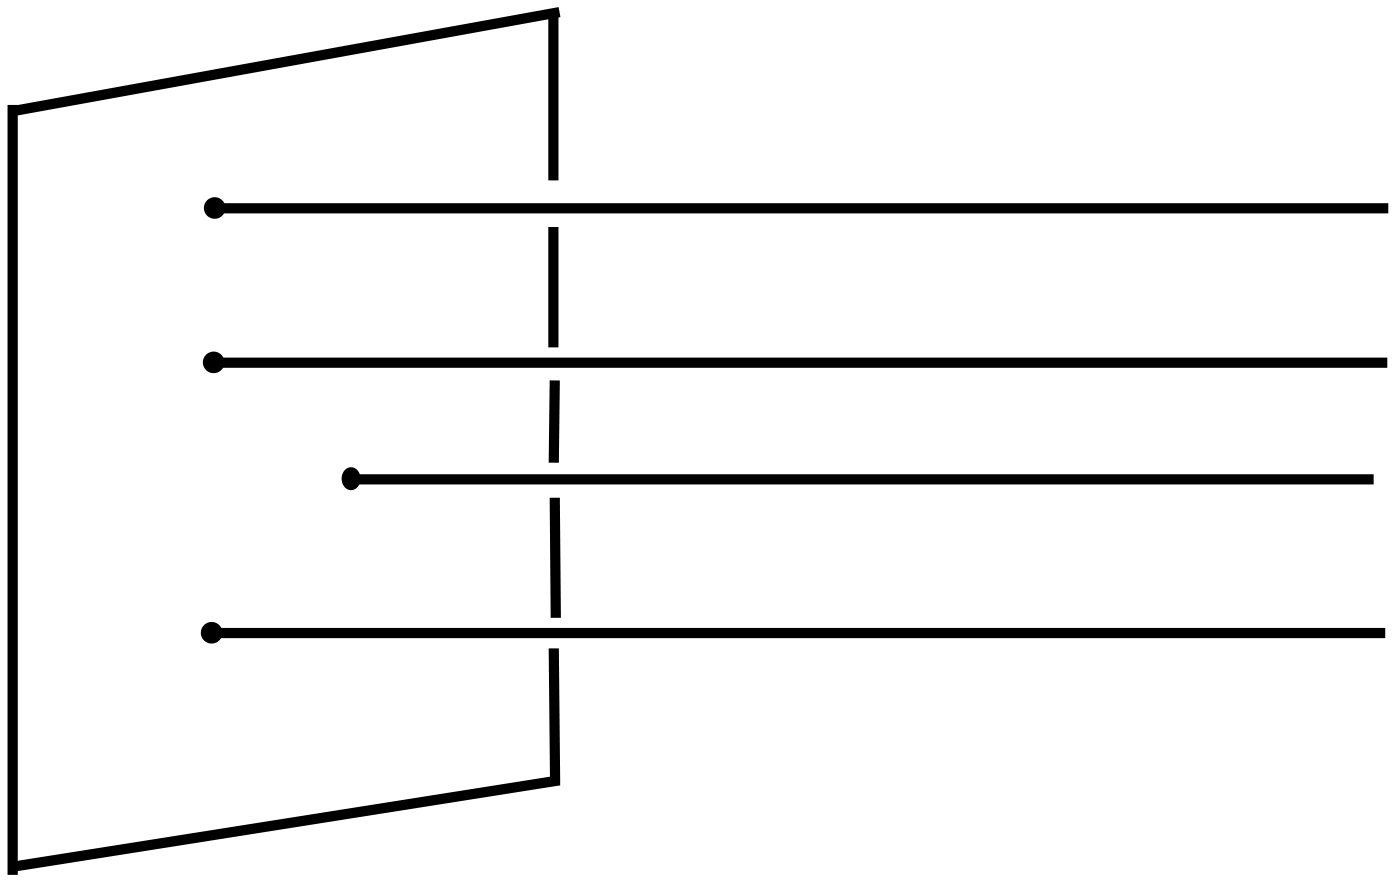
\includegraphics[width=3.5in]{figs/Fig26.png}
 \end{center}
\caption{\small  $C\times \R_+$ 中的单值性缺陷，支撑在 $p_i\times \R_+$ 上，其中 $p_i$ 是 $C$ 中的点。$C$ 用矩形表示。我们假定 $y=0$ 处有 Nahm 极点边界条件。（原稿第 104 页）}
 \label{defects}
\end{figure}
我们要考虑的第一个膜是 oper 膜。它照例由 Nahm 极点边界条件定义。为此取 $\Sigma$ 为 $\R\times \R_+$，其中 $\R_+$ 是通常的半直线 $y\geq 0$，并在 $y=0$ 处施加 Nahm 极点边界条件。略去 $\R$ 即时间方向，$C\times \R_+$ 上的图像如图~\ref{defects} 所示：有支撑在 $p_i\times \R_+$ 上的单值性缺陷，各自带有参数 $(\alpha_i,\beta_i,\gamma_i,\eta_i)$，以及 $y=0$ 处的 Nahm 极点边界条件。当然，我们需要解释：当单值性缺陷终止于带 Nahm 极点的边界上时，我们想要的是何种奇点。一如往常，这类问题可以通过寻找具有所需奇点的模型解来回答。就目前情形而言，文献~\cite{fiveknots} 第 3.6 节已经做了这件事，文献~\cite{Mikhaylov} 则给出了更一般的处理。

设 $\alpha-i\gamma=\lambda\,\mathrm{diag}(i,-i)$，$\lambda$ 为复参数，并考虑在（比如）$z=0$ 处具有这类奇点的希格斯丛 $E$。若 $E$（在复结构 $I_\zeta$ 中看）同时也是一个 oper，则它可由经典应力张量
\begin{equation}\label{lork}t=-\frac{\lambda(\lambda+1)}{z^2}+\dots, \end{equation}
描述，其中我们略去了奇异性更弱的项。这个公式与 (\ref{roog}) 相似，只是把 $j_a=k_a/2$ 换成了 $\lambda$。$E$ 的平坦截面对应于微分方程
\begin{equation}\label{stork}\left(\frac{\partial^2}{\partial z^2}+t\right)\psi=0.\end{equation}
的全纯解。对一般的 $\lambda$，可以找到两个线性无关的解，$\psi_1=z^{-\lambda} \left(1+\sum_{i=1}^\infty c_iz^i\right)$，$\psi_2=z^{\lambda+1}\left(1+\sum_{i=1}^\infty \tilde c_i z^i\right)$。这意味着，正如预期，单值性为
\begin{equation}\label{dusc}U=\mathrm{diag}(\exp(-2\pi i\lambda),\exp(2\pi i\lambda)).\end{equation}

% [Tutor Note: 物理图像] (\ref{lork}) 中的组合 $-\lambda(\lambda+1)/z^2$ 正是二维共形场论中“权重为 $j=-\lambda-1$ 与 $j=\lambda$ 的退化场”所对应的应力张量零点结构（比较 (\ref{roog}) 中 $j_a=k_a/2$ 的情形），它保证 (\ref{stork}) 有 $z^{-\lambda}$ 与 $z^{\lambda+1}$ 两个解，指数之和为 1。$\lambda\to k/2$ 时两指数之差 $2\lambda+1\to k+1$ 成为整数，于是出现对数解——这正是下一段要处理的情形。

若改为取 $\lambda=k/2$，$k\in \Z$，会怎样？此时总存在解 $\psi_2=z^{k/2+1}(1+\sum_{i=1}^\infty \tilde c_iz^i)$，但若我们寻找形如 $\psi_1=z^{-k/2}(1+ c_1z+\dots)$ 的解，就会发现：一般地，当把该展开推进到 $z^{k/2+1}$ 阶时，我们需要量级为 $ z^{k/2+1}\log z+\dots$ 的对数项。对数项恰好是 $(\log z)\psi_2$ 的某个倍数。相应地，绕 $z=0$ 的单值性一般地取幂幺形式
\begin{equation}\label{omogg}
\begin{pmatrix} \psi_1\cr \psi_2\end{pmatrix}\to (-1)^k\begin{pmatrix} 1 &  s\cr
    0 & 1\end{pmatrix}\begin{pmatrix}\psi_1 \cr \psi_2\end{pmatrix}\end{equation}
    其中 $s$ 为某个复常数。

因此，若要使绕 $z=0$ 的单值性为平凡，我们需要对 (\ref{lork}) 应力张量的次领头系数施加一个条件，以使 $s=0$。这意味着：绕 $z=0$ 的单值性平凡是一个中间维数的条件。确实，若无此条件，$G=SU(2)$ 的单值性缺陷使 $\M_H$ 的复维数增加 2，而平凡单值性条件固定这 2 个参数中的 1 个。

% [Tutor Note: 省略论证] 作者说“$s=0$ 是对次领头系数的一个条件”而未写出显式公式：具体地，$s$ 是应力张量中 $1/z$ 阶项（即 $t=-k(k+2)/(4z^2)+t_{-1}/z+\dots$ 中的 $t_{-1}$）的线性函数；把 (\ref{stork}) 的 Frobenius 级数推进到对数阶即可解出 $s\propto t_{-1}$。因此“平凡单值性”在参数空间中确实是一个余维 1 的条件，这正是“中间维数”的定量含义。

这一点很重要，我们稍作展开。一般地，绕缺陷的单值性是 $SL(2,\C)$（复维数 3）中满足一个约束（指定其共轭类）的元素，从而剩下 2 个复参数。例如当 $\alpha=\gamma=0$ 时，该共轭类是二维的，正如 (\ref{onk}) 所显式展示的那样。平凡单值性条件（仅当 $U=\exp(-2\pi(\alpha-i\gamma))$ 等于 $\pm 1$ 时才有定义，对其他取值没有类似物）固定与缺陷相联系的 2 个参数中的 1 个，于是剩下 1 个参数。可以把这 1 个参数看作式 (\ref{justo}) 中 $\beta \,\d r/r$ 项所对应的对称破缺方向。对称破缺方向的选取确定了一副本 $\CP^1$ 中的一个点；这个 $\CP^1$ 是 $E$ 在单值性缺陷所在点 $p\in C$ 处的纤维的射影化。关于这个 $\CP^1$ 之来历的更详细解释如下。首先，由于方程 $x^2+yz=0$，式 (\ref{onk}) 所描述的幂幺共轭类作为复流形显式同构于 $\C^2/\Z_2$，在 $x=y=z=0$ 处有 $\sf A_1$ 奇点。该奇点正是 (\ref{onk}) 中群元 $V$ 等于 $\pm 1$ 的那个点。在把 $\M_H$ 构造为 hyper-Kähler 流形的框架中，$\beta$ 参数是吹开 $\sf A_1$ 奇点的 Kähler 参数，它把共轭类 $\C^2/\Z_2$ 换成其消解，即 Eguchi-Hansen 流形 $T^*\CP^1$。在吹开中，原点处的奇点被一份 $\CP^1$ 取代。关于 $\beta$ 作为吹开参数的解释见文献~\cite{Simpson}，关于其中若干事情的从容解说见文献~\cite{GuW}。

% [Tutor Note: 原文用词] 原文写作 “Eguchi-Hansen manifold”，通行拼法为 Eguchi-Hanson（埃古奇–汉森空间）。此处按原文保留，未作改动；它指 $T^*\CP^1$ 作为 $\C^2/\Z_2$ 的极小消解所带的 hyper-Kähler 度规。

我们实际上已经遇到过如下事实：在这一情形中，单值性消失是一个中间维数的条件。我们专门考虑 $C=\CP^1$ 的情形（我们也可以类似地处理 $C=\C$ 且在无穷远处有非正则奇点的情形）。由第~\ref{opbethe}~节我们知道，对给定的一组奇点 $z_a$ 与磁荷 $k_a$，$a=1,\dots,d$，只有有限多个具有无单值性奇点的 oper。平坦 $G_\C$ 丛成为 oper 这一条件是中间维数的条件。要归约为有限多个具有无单值性奇点的 oper，单值性消失的条件也必须同样是中间维数的。（这一断言暗中假定两个条件以横截的方式相交，事实确实如此。）

事实上，若放弃 oper 条件，我们可以显式描述 $C$ 上 Hitchin 方程解构成的模空间，其中单值性缺陷由 $\lambda_a=k_a/2$ 刻画，且复联络 $\A$ 绕这些点的单值性平凡。由于 $C$ 单连通，$C$ 上绕各点 $p_a$ 无单值性的平坦丛作为平坦丛是完全平凡的。唯一可能的模来自与参数 $\beta_a$（我们假定全部非零）相联系的对称破缺：它在每个奇点 $p_a$ 处生成一份 $\CP^1$。要得到模空间，必须把这些 $\CP^1$ 的乘积除以平凡平坦丛 $E$ 的自同构群；后者是一份 $SL(2,\C)$。于是最终，Hitchin 方程在各奇点处单值性平凡的平坦丛所对应的解构成的轨迹 $\mathcal U$ 同构于 $(\CP^1)^d/SL(2,\C)$。这是 $\M_H$ 在复结构 $J$ 下的一个复子流形（它由对单值性的条件定义，而单值性在该复结构下是全纯的）。其维数为 $d-3$，恰为 $\M_H$ 维数的一半。事实上，从复结构 $J$ 的角度看 $\mathcal U$ 是复 Lagrangian 的；这大致是因为每份 $\CP^1 $ 在 $T^*\CP^1$ 中都是复 Lagrangian 的。因此，支撑在 $\mathcal U$ 上、带平凡 Chan-Paton 丛的膜 $\Btriv$ 是 $(A,B,A)$ 型的半 BPS 膜。

% [Tutor Note: 易错点] 维数核对：$(\CP^1)^d$ 复维数 $d$，除以 $SL(2,\C)$（复维数 3）得 $d-3$。而 $\M_H$ 对 $G=SU(2)$ 的复维数为 $6(g-1)+2d=2d-6$（$g=0$，$d$ 个正则奇点），其一半正是 $d-3$。注意此处 $g=0$ 时先要 $d\ge3$ 才能整除得到正维数，这与前文“亏格 0 需 3 个单值性缺陷”的说法一致。

这给了我们思考平凡单值性 opers 的新方式。它们是两个 $(A,B,A)$ 型 Lagrangian 子流形的交点——一个流形是 opers 簇，另一个参数化具有平凡单值性的丛。因此，平凡单值性 opers 给出拉伸在膜 $\Boper$ 与膜 $\Btriv$ 之间的超对称开弦空间的一组基。我们称这个空间为 $(\Boper,\Btriv)$ 弦空间。技术上，这里我们要的是 $J$ 型 $B$ 模型中的 $(\Boper,\Btriv)$ 弦空间。

我们可以利用 $S$ 对偶来研究这个超对称弦态空间，$S$ 对偶把 $J$ 型 $B$ 模型转换为 $\omega_K$ 型 $A$ 模型。正如第~\ref{sduality}~节所知，$S$ 对偶把膜 $\Boper$ 转换为典范余迷向膜 $\Bcc$。结果表明（我们将很快描述），$\Btriv$ 在 $S$ 对偶下映为自身（单值性缺陷参数 $(\alpha_a,\beta_a,\gamma_a,\eta_a)$ 按通常方式变换）。因此 $(\Boper,\Btriv)$ 弦空间的 $S$ 对偶就是 $(\Bcc,\Btriv)$ 弦空间，只不过现在是在 $\omega_K$ 型 $A$ 模型中看。这个问题的关键之处在于：虽然 $\Btriv$ 的支撑对 $\omega_K$ 是 Lagrangian 的，但它对 $\omega_J$ 实际上是辛的——确实，$\Btriv$ 的支撑是复结构 $J$ 下的复子流形，因而以 $\omega_J$ 为其 Kähler 形式。既然如此，描述 $(\Bcc,\Btriv)$ 弦空间的问题就由文献~\cite{GuWtwo} 中关于量子化与膜的分析所支配。$(\Bcc,\Btriv)$ 弦空间通过量子化 $\Btriv$ 的支撑 $\mathcal U$ 得到；这里 $\mathcal U$ 被视为带辛结构 $\omega_J$ 的辛流形。



 \begin{figure}
 \begin{center}
     % >>> 原文图 27（原稿第 106 页）
  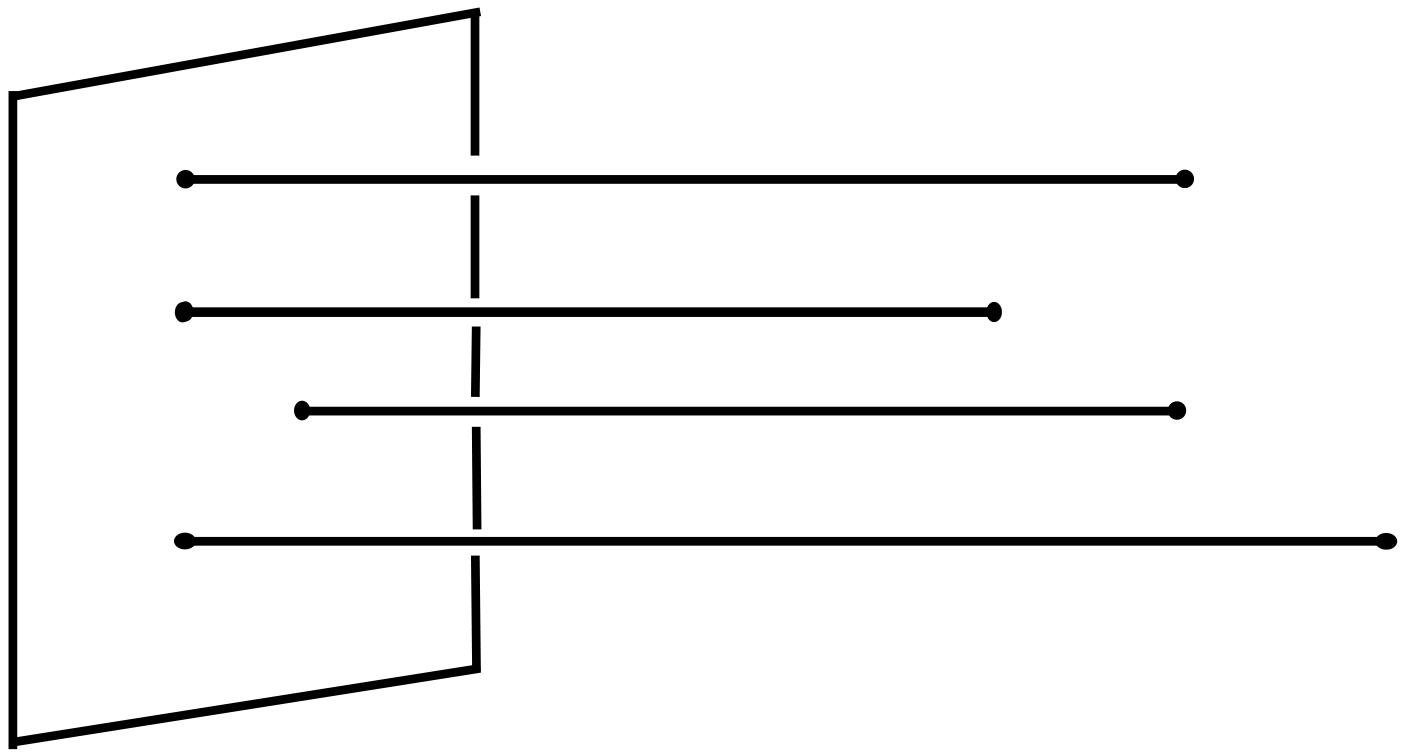
\includegraphics[width=3.5in]{figs/Fig27.png}
 \end{center}
\caption{\small  本图与图~\ref{defects} 的唯一区别在于：每条单值性缺陷线都终止于一个奇异磁单极子，即右侧的黑点。由于缺陷线本身是自对偶的（在参数作适当变换之后），由缺陷线终止所定义的膜也是自对偶的。（原稿第 106 页）}
 \label{ends}
\end{figure}

\subsection{一个自对偶膜}\label{simplex}
关于 $\Btriv$ 为何自对偶，有一个简单的规范理论解释。暂时不管超对称，我们可以把单值性缺陷线看作与一个可能未被正确量子化的磁单极子相联系的 Dirac 弦。因此，单值性缺陷线可以终止于一个奇异磁单极子（图~\ref{ends}）。由于单值性缺陷在 $S$ 对偶下映为自身（参数作某种变换），单值性缺陷终止于奇异磁单极子的图像在 $S$ 对偶下也类似地映为自身。

超对称对这类图像得以存在的参数取值施加了一些约束。在 $J$ 型 $B$ 模型的框架中，若缺陷线要终止，则绕给定缺陷线的单值性必须平凡。这意味着，在这个 $B$ 模型中，图~\ref{ends} 的图像只有在 $\alpha=\gamma=0$ 时才存在（这里我们把 $\alpha$ 与 $\eta$ 视为周期变量）。当然，无论如何那都是 $\Btriv$ 得以定义的情形。对偶地，在 $\omega_K$ 型 $A$ 模型中，像图~\ref{ends} 那样的图像只有在 $\gamma=\eta=0$ 时才存在。（例如，$\eta$ 必须为零，因为若单值性缺陷的支撑终止于沿该缺陷的 $U(1)$ 丛未被平凡化的地方，则世界面 theta 角 $\eta$ 就不能保持 $A$ 模型的拓扑超对称。）



在本文的框架中，具有平凡单值性的 opers 最直接地来自 $y=0$ 处的奇异磁单极子。不过，在不改变任何本质内容的前提下，我们可以把奇异磁单极子移离边界，只要用单值性缺陷把它们与边界相连，如图~\ref{ends} 那样。这样做的好处是：它使“平凡单值性 opers 是两个膜的交点”这一点变得显然，也使其中一个膜的自对偶性变得清楚。

在缺陷线终止于奇异磁单极子的一般情形中，该磁单极子可能被错误地量子化。然而对 $\lambda=k/2$，它等价于 $\gamma=0$、$\alpha=(k/2)\mathrm{diag}(i,-i)$，此时弦末端的磁单极子服从 Dirac 量子化，但该弦是可观测的，因为我们假定 $\beta\not=0$。
   % §8  oper 与膜（前半）
\subsection{在 Gaudin 模型中的应用}\label{applic}

膜 $\Btriv$ 的自对偶性为文献~\cite{FFR,Frenkel} 的主要结果提供了一个规范理论解释：$\CP^1$ 上具有平凡单值性的 opers 对应于 Gaudin 模型对易哈密顿量的同时本征向量。我们考虑 $(\Bcc,\Btriv)$ 弦空间与 $(\Boper,\Btriv)$ 弦空间之间的对偶。以下讨论假定读者熟悉文献~\cite{GuWtwo} 的框架。

% [Tutor Note: 物理图像] 这里的逻辑链是：$(\Bcc,\Btriv)$ 弦的量子化给出 $\frak H=(\otimes_aR_a)^{SU(2)}$，而对易 Hamiltonians 作为 $(\Bcc,\Bcc)$ 弦作用于其上；$S$ 对偶把该问题换成 $(\Boper,\Btriv)$ 弦，后者在 $B$ 模型中就是两个经典膜的交点，于是“本征向量”变成“交点”，即具有平凡单值性的 opers。这就是 Gaudin 模型可积结构与 oper 几何之间的对偶的物理来源。

为构造 $(\Bcc,\Btriv)$ 弦空间，我们必须量子化模空间 $(\prod_{a=1}^d\CP^1_a)/SL(2,\C)$，其中 $\CP^1_a$ 是附着在 $z=z_a$ 处单值性缺陷上的一份 $\CP^1$。$\CP^1_a$ 的量子化给出 $SU(2)$ 的一个不可约表示 $R_a$，其自旋为 $j_a=k_a/2$；而 $(\prod_{a=1}^d\CP^1_a)/SL(2,\C)$ 的量子化给出一个量子 Hilbert 空间 $\frak H$，它是 $\otimes_a R_a$ 的 $SU(2)$ 不变部分，
\begin{equation}\label{ifo} \frak H=(\otimes_aR_a)^{SU(2)}. \end{equation}
Hitchin 可积系统的经典对易哈密顿量可以（在 $\omega_K$ 型 $A$ 模型中）解释为 $(\Bcc,\Bcc)$ 弦。因此它们作用于 $(\Bcc,\Btriv)$ 弦的空间 $\frak H$ 上。事实上，Hitchin 哈密顿量成为 Gaudin 模型的对易哈密顿量。为证明后一陈述，我们把 $R_a$ 上 $SU(2)$ 作用的生成元解释为来自 $\CP^1_a$ 上的一阶微分算子，于是 Gaudin 哈密顿量 (\ref{gaudham}) 成为二阶微分算子。这些算子的“符号”（即领头项的系数）是 Hitchin 纤维化底空间上的函数，而这些函数正是 Hitchin 哈密顿量。因此反过来读，Gaudin 哈密顿量表示 Hitchin 哈密顿量的一个量子化（而且鉴于 Hitchin 哈密顿量彼此对易，这一量子化在相差添加 $c$-数的意义下是唯一的）。

% [Tutor Note: 易错点] “量子化 $\CP^1_a$ 得到自旋 $j_a=k_a/2$ 的表示”用的是几何量子化：$\CP^1$ 的辛形式取为曲率 $\propto$ 面积形式，其预量子化线丛的次数即 $2j_a$，故 $2j_a=k_a$。若把 $\CP^1_a$ 的辛形式归一化取反或取倍，$j_a$ 会差整数倍，进而使 $\frak H$ 与 Gaudin 模型的谱不匹配；此处必须以第~\ref{mondr}~节中 $\lambda_a=k_a/2$ 的定义为准。

为理解对易哈密顿量的本征向量与本征值，我们利用 $\omega_K$ 型 $A$ 模型中的 $(\Bcc,\Btriv)$ 弦与 $J$ 型 $B$ 模型中的 $(\Boper,\Btriv)$ 弦之间的等价性。后一类弦简单地对应于经典膜 $\Bcc$ 与 $\Boper$ 的交点。因此，具有平凡单值性的 opers 给出 Gaudin 模型的量子 Hilbert 空间 $\frak H$ 的一组基。在 $B$ 模型的描述中，对易哈密顿量简单地成为 opers 簇 $\V$（即膜 $\Boper$ 的支撑）上的函数。Hitchin 的经典哈密顿量是 $C$ 上二次微分空间（在单值性缺陷位置 $z_a$ 处具有指定类型的极点）上的全纯函数。$\V$ 的支撑是 $C$ 上的应力张量空间（在 $z_a$ 处具有指定极点）。应力张量空间与二次微分空间之差仅在于 $c$-数的共形反常。这与 Hitchin 哈密顿量量子化中的加性 $c$-数不确定性相匹配。对应于给定 oper 的量子化哈密顿量的本征值，简单地由与该 oper 相联系的应力张量给出。

最近文献~\cite{NStwo} 描述了一种 Gaudin 模型的“非紧”版本，其中有限维表示 $R_a$ 被无限维表示取代。对易哈密顿量的本征向量再次用 opers 表达，只是对其单值性有某些条件。自然可以猜测这一构造同样反映了某个自对偶膜的存在。确实有一个很好的候选者——一个自对偶膜，它通过把单值性缺陷的端点（如图~\ref{ends} 那样）换成这类缺陷的汇合点来构造，如图~\ref{junctions} 那样。这样的汇合点由如下方式定义：取一个环绕该汇合点的小二维球面 $S$，在其上求解 Hitchin 方程，并在 $S$ 与各单值性缺陷的交点处具有奇点（奇点类型依赖于参数 $\alpha_a,\beta_a,\gamma_a,\eta_a$）。



 \begin{figure}
 \begin{center}
     % >>> 原文图 28（原稿第 108 页）
  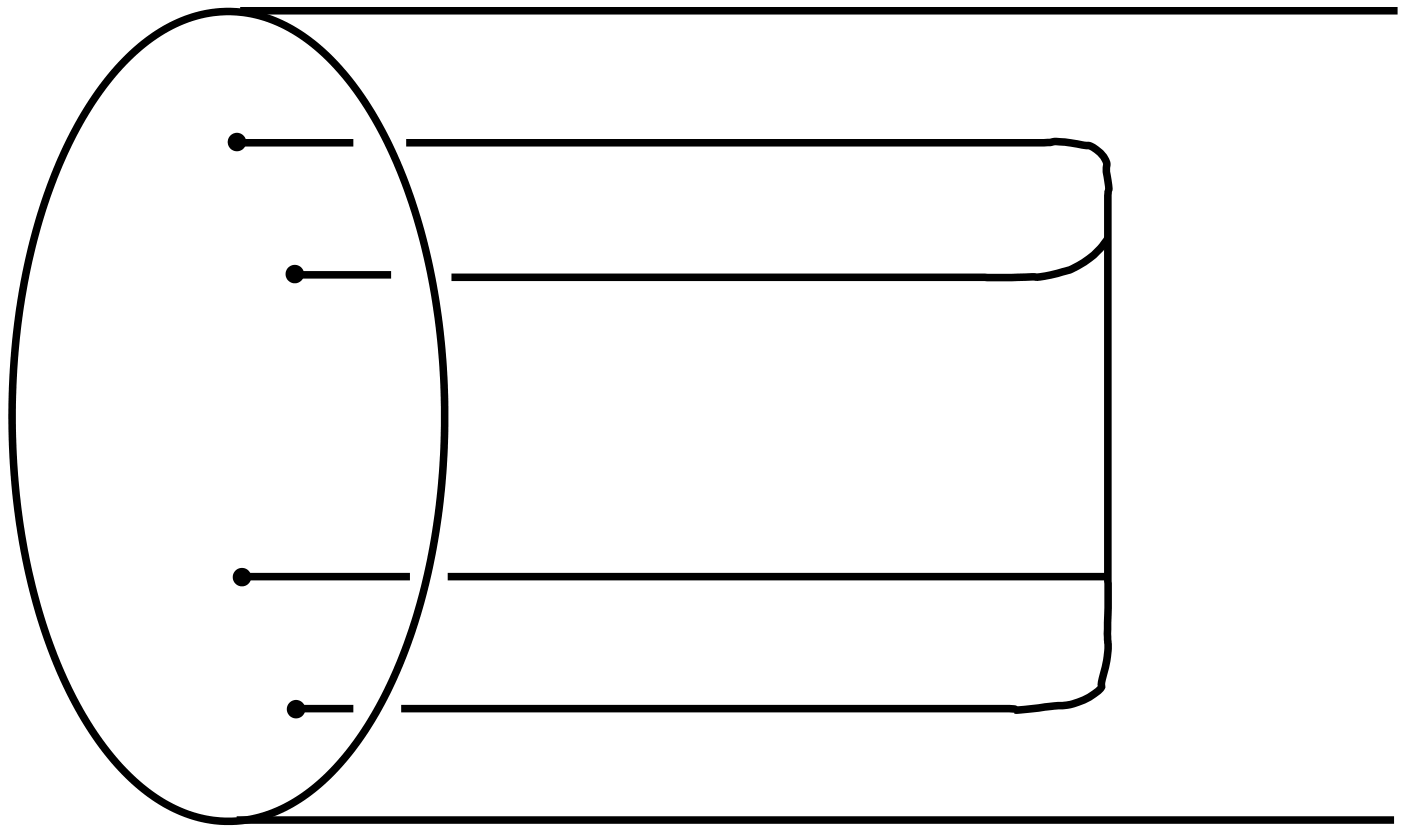
\includegraphics[width=3.5in]{figs/Fig28.png}
 \end{center}
\caption{\small  另一个自对偶膜可以通过把我们在图~\ref{ends} 中用到的单值性缺陷端点替换为单值性缺陷的汇合点来构造，如图所示。（原稿第 108 页）}
 \label{junctions}
\end{figure}

\vskip .5cm
{\bf 致谢} 我们感谢 D. Bar-Natan、L. Kauffman、S. Lewallen、P. Li、R. Mazzeo、G. Moore、R. Schoen、P. Seidel、L.-F. Tam 与 V. Toledano-Laredo 的讨论与评论。我们也感谢 M. Turansick 在作图方面的协助。

\appendix


\section{从六维得到的三维 BPS 方程}\label{fromsix}

\begin{keytakeaways}
\begin{itemize}\setlength{\itemsep}{2pt}
  \item \textbf{物理图像}：三维 BPS 方程可以由六维理论得到：要求场强（视为 $SO(6)$ 李代数元素）落在某个 $SU(3)$ 子代数内，再作维数约化；不同的 $SU(3)$ 嵌入在约化后给出不等价的三维方程族。
  \item \textbf{数学工具}：$SO(6)/U(3)\sim SU(4)/U(3)\sim \CP^3$ 参数化 $SU(3)\subset SO(6)$ 的嵌入，$SO(3)\times SO(3)$ 的转动作用（在六维旋量空间上即 $SO(4)\subset SU(4)$），Nahm 方程与 Nahm 极点。
  \item \textbf{主要结论}：方程族是实一维的，$(\ref{bpszeta})$ 是其一般代表；$\zeta$ 可通过 $SO(2)_\zeta$ 旋转改变（代价是 $\varphi$ 的 $(1+\zeta^2)$ 标度变换），旋转后的 Nahm 极点边界条件由此得到；$\zeta$ 的几何意义体现在 moment map 的系数矩阵 $\omega^{ab}$ 上，且 $\omega^{z \bar z}/\omega^{\bar z z}=\zeta^2$。
\end{itemize}
\end{keytakeaways}

我们在第~\ref{teqone}~节考虑的时间无关位形是三维 BPS 方程
\begin{equation} \label{sixbps}
[\D_i, \D_j]=0 \qquad  \sum_{i=1}^3[\D_i,\D_i{}^\dagger]
\end{equation}
的解，其中的三维联络与三个伴随标量场被一起打包进算子 $\D_i$：
\begin{align} \D_1 & = \frac{D}{Dx^2}+i\frac{D}{Dx^3}    \cr
                                   \D_2 & = [\phi_2-i\phi_3,\,\cdot\,] \cr
                             \D_3 & = \frac{D}{Dy}-i[\phi_1,\,\cdot\,]  \end{align}
或者用复记号写成
\begin{align}\label{oggi} \D_1 & =2\frac{D}{D\bar z} \cr
                                                              \D_2 & = 2[\varphi,\,\cdot\,]\cr
                                                               \D_3& = \frac{\D}{\D y}. \end{align}
该方程组可以推广为含一个实参数的三维 BPS 方程族，其形式与 \ref{sixbps} 相同，但算子 $\D_i$ 的选择不同：
\begin{align}\label{bpszeta}\D_1 & =2\frac{D}{D\bar z}  +2 \zeta [\bar \varphi,\,\cdot\,] \cr
                                                              \D_2 & = - 2 \zeta \frac{D}{D z} + 2[\varphi,\,\cdot\,]\cr
                                                               \D_3& = \frac{\D}{\D y}. \end{align}
这一推广曾在第~\ref{analog}~节研究过。



这一族三维方程可以从六维有效地导出。我们从坐标 $x^a,$ $x^{a+3}$（$a=1,2,3$）的 $\R^6$ 出发，然后对规范场施加约束：要求场强（视为 $SO(6)$ 李代数中的元素）落在某个指定的 $SU(3)$ 子群内。只要还在六维中，子群的选择就无关紧要；它只相当于选定 $\R^6$ 与 $\C^3$ 的一个等同方式。但若我们要求各场实际上只依赖于前三个坐标 $x^a$，并在 $x^{a+3}$ 的常数平移下不变，那么 $SU(3)$ 子群的选择就变得重要了。因此在约化到三维之后，可以得到一个依赖于参数的、彼此不等价的三维方程组族。



要说明该族（模去等价）是实一维的，一个简单办法如下。首先，$SU(3)$ 在 $SO(6)$ 中的嵌入选择由 $SO(6)/U(3)\sim SU(4)/U(3) \sim \CP^3$ 参数化，它等价于在正手征的六维旋量空间中选定一条复直线。约化到三维后，不等价的三维方程组由这样的选择模去空间转动与三个标量 $\phi_i$ 转动的 $SO(3) \times SO(3)$ 群参数化。虽然该群与 $\CP^3$ 一样是六维的，但它在 $\CP^3$ 上的作用并不自由；相反，$\CP^3$ 中的一般点保持 $SO(3)\times SO(3)$ 的一个 $SO(2)$ 子群。例如，由 $\zeta$ 参数化的所有三维方程在 $D/Dz$ 与 $\phi_z$ 同时作相位转动下不变。一般地，$SO(3) \times SO(3)$ 在六维旋量空间上的作用相当于 $SO(4) \subset SU(4)$。因此 $SU(4)$ 的一个复旋量是 $SO(4)$ 的一个复向量，其实部与虚部分别把 $SO(4)$ 破缺到 $SO(2)$。于是，作为六维方程的维数约化而得到的三维方程组族是实一维的，而 (\ref{bpszeta}) 是一般的代表。

这一图像的一个推论是，我们可以用 $SO(6)$ 转动来改变 $\zeta$。确实，通过作用一个我们记作 $SO(2)_\zeta$ 的群中的适当元素，就可以按需要改变 $\zeta$；该群把 $D/Dx^2$ 与 $[\phi_2,\,\cdot\,] $ 相互转动，也把 $D/Dx^3$ 与 $[\phi_3,\,\cdot\,]$ 相互转动。确切地说，作用在 $\zeta=0$ 处定义的 $\D_i$ 上的 $SO(2)_\zeta$ 转动将给出略微标度过的 $\D_i$，带一个前因子 $(1+\zeta^2)^{-1/2}$。该前因子可以通过对 $z$ 坐标作简单的标度变换而吸收掉。

现在我们讨论本文中十分重要的 Nahm 极点边界条件。若假定各场只依赖于 $y$，并进一步假定 $A_{\bar z}=0$（从而可以不顾 $\D_1$），则取 (\ref{oggi}) 中 $\D_i$ 的方程 (\ref{sixbps}) 约化为 Nahm 方程。Nahm 极点边界条件定义为要求 $y\to 0$ 时各场可以用 Nahm 方程的某个奇异解来近似。


对一般 $\zeta$ 的三维 BPS 方程也有类似的边界条件。确实，$SO(2)_\zeta$ 把只依赖于 $y$ 的 (\ref{sixbps}) 的解映为只依赖于 $y$ 的 (\ref{bpszeta}) 的解。更显式地，取 (\ref{bpszeta}) 中 $\D_i$ 的一般形式，我们可以寻找只依赖于 $y$、且使 $\D_1$ 约化为 $2\partial/\bar\partial\bar z$ 的解，即 $A_{\bar z} =- \zeta \bar \varphi$。于是 $\D_2 =  2(1 + \zeta^2) [\varphi,\,\cdot\,]$，从而我们可以把 Nahm 方程的解嵌入为一般三维 BPS 方程的解，代价是把复标量 $\varphi$ 标度 $1+ \zeta^2$ 倍。这就引出了我们在本文中发现有用的旋转后 Nahm 极点边界条件。

% [Tutor Note: 原文笔误] 此处原文作 “$\D_1$ reduces to $2\partial/\bar\partial\bar z$”，按上下文与 $\D_1=2D/D\bar z$（$D/D\bar z=\partial/\partial\bar z+[A_{\bar z},\,\cdot\,]$，当 $A_{\bar z}=-\zeta\bar\varphi$ 时其纯导数部分为 $2\partial/\partial\bar z$）判断，应为 $2\partial/\partial\bar z$。原式如此，未改。

当然，我们刚才描述的并非与一般三维 BPS 方程相容的唯一 Nahm 极点嵌入方式。例如，在 $\zeta \neq 0$ 时，我们本可以选择另一种嵌入，使 $\D_2$ 而非 $\D_1$ 是平凡的；那将引出我们或可称为反 opers 的对象——即平坦丛，其 oper 型约束加在反全纯结构而非全纯结构上。把我们所选的 Nahm 极点用 $SU(3)$ 中保持 $\D_3$ 的 $U(2)$ 子群作任意转动，都会产生一个可能的边界条件，但我们将一般坚持用“oper”型 Nahm 极点。

最后，我们对参数 $\zeta$ 的含义给出另一种解释。对有限非零的 $\zeta$，可以对 $\D_i$ 作标度变换，并将其解释为一般的复三维联络。在直角坐标中，可把联络的各分量记为 $\tilde \D_a$。复方程告诉我们该联络是平坦的。然后我们有一个 moment map 约束，它令对易子 $[\tilde \D_a, \tilde \D^\dagger_b]$ 的某个常系数线性组合为零。

从这一观点看，$\zeta$ 只出现在 moment map 方程的选取中。对易子的一般线性组合由系数构成的 $3 \times 3$ 矩阵 $\omega^{ab}$ 描述，
\begin{equation}\label{mct}  \sum_{a,b} \omega^{ab} [\tilde \D_a,\tilde \D_b{}^\dagger]=0.
\end{equation}
由式 (\ref{bpszeta}) 可得一个有用的关系：$\omega^{z \bar z}/\omega^{\bar z z}=\zeta^2$。若 $\zeta^2=1$，则 $\omega^{ab}$ 是对称的，但一般并非如此。

一般地，在线性坐标重定义下，可能的 $\omega^{ab}$ 构成一个一维参数空间。例如，若 $\omega^{ab}$ 的对称部分是正定的（对 (\ref{bpszeta}) 而言确实如此），我们可以把它化为单位矩阵 $\delta^{ab}$。此时反称部分 $B^{ab}$ 可以转动到只存在于 $z, \bar z$ 平面内，其大小由一个实参数控制，我们可以把这个参数等同于 $\zeta$。

\section{从四维与八维得到的三维 BPS 方程}\label{foureight}

\begin{keytakeaways}
\begin{itemize}\setlength{\itemsep}{2pt}
  \item \textbf{物理图像}：四维 BPS 方程 (\ref{bpseqns}) 可看作八维 Yang-Mills 中 BPS 方程的维数约化；把 $x^1$ 方向去掉并把 $A_1,\phi_y$ 取为 $\vec\phi$ 的线性组合，就得到三维 BPS 方程，其参数 $\zeta$ 由该组合决定。
  \item \textbf{数学工具}：八维 $\mathrm{Spin}(8)$ 手征旋量 $\epsilon$、条件 $F_{IJ}\Gamma^{IJ}\epsilon=0$、$\mathrm{Spin}(7)\subset SO(8)$ 与 $SO(6)\to SU(3)$ 的嵌入链、升降算符 $\gamma_{\underline a},\gamma_{\overline a}$ 与真空 $|\Omega\rangle,|\mho\rangle$、$\tau=\tan\alpha$。
  \item \textbf{主要结论}：四维方程 (\ref{dolk}) 由八维方程约化得到且 $\t=\tan\alpha$；只依赖于部分坐标的解保持额外超对称（$F_{I8}=0$ 给出 $SO(7)\to G_2$；再加上 $F_{I7}=0$ 给出 $SO(6)\to SU(3)$ 及三维 BPS 方程）；显式做法是绕 $(a,a+4)$ 平面作 $SO(2)$ 转动，$\zeta=\tan\theta_2$，且取 $\theta_1=-2\theta_2=-2\theta_3=-2\theta$ 时保持 $\t=1$、只形变 Nahm 极点边界条件。
\end{itemize}
\end{keytakeaways}

在本附录中，我们将讨论参数为 $\zeta$ 的三维 BPS 方程如何能从四维 BPS 方程 (\ref{bpseqns}) 的时间无关解得到。我们将推广如下陈述：三维中 $\zeta=0$ 的方程来自四维中 $\t=1$ 的方程，只要我们丢掉对某个坐标（比如 $x^1$）的依赖，并令 $A_1=\phi_y=0$。

首先我们将说明这并不是某个特定选择所特有的性质。我们可以从任意 $\t$ 出发，令 $\d/\d x^1=0$，并把 $A_1$ 与 $\phi_y$ 取为 $\phi$ 的其余三个分量的任意两个线性组合，则所得的三维方程将等价于上一附录中讨论的三维 BPS 方程，对 (\ref{bpszeta}) 中参数 $\zeta$ 的某个取值成立。

为此，把四维 BPS 方程改写为紧致形式（即八维 Yang-Mills 理论中 BPS 方程的维数约化）相当方便。描述所需八维方程的一个简洁方式是：取一个具有确定手征性的 $\mathrm{Spin}(8)$ 旋量 $\epsilon$，并要求
\begin{equation}
F_{IJ} \Gamma^{IJ} \epsilon =0.
\end{equation}
若把曲率 $F_{IJ}$ 理解为 $SO(8)$ 李代数中的元素，则这些方程把曲率限制在 $SO(8)$ 的 $\mathrm{Spin}(7)$ 子代数中。由于如下显然的关系，这些其实只是 7 个方程：
\begin{equation}
\epsilon^T F_{IJ} \Gamma^{IJ} \epsilon =0,
\end{equation}
因为 $\Gamma^{IJ}$ 是反称的。

约化到四维把 $SO(8)$ 破缺为一个我们记作 $SO(4)_s \times SO(4)_R$ 的子群，它分别作用在前四个与后四个坐标上。旋量 $\epsilon$ 分解为在 $SO(4)_s$ 与 $SO(4)_R$ 下均为左手征的一片 $\epsilon_L$，以及在 $SO(4)_s$ 与 $SO(4)_R$ 下均为右手征的一片 $\epsilon_R$。若 $\epsilon_L$ 与 $\epsilon_R$ 都非零，则它们选定一个对角地嵌在 $SO(4)_s \times SO(4)_R$ 中的扭化 $SO(4)'_s$，使得 $\epsilon_L$ 与 $\epsilon_R$ 都是 $SO(4)'_s$ 标量。于是那 $7$ 个方程在 $SO(4)'_s$ 下分解为三个自对偶二形式、三个反自对偶形式和一个标量方程。这正是 (\ref{bpseqns}) 中熟悉的形式。


\def\a{{\underline a}}
\def\aa{{\overline a}}
\def\b{{\underline b}}
\def\bb{{\overline b}}
我们把 $a'$ 作为 $a+4$ 的简写，并采用复记号，其中 $\a$ 是 $a+ia'$ 的简写，$\aa$ 是 $a-ia'$ 的简写。为把八维方程显式地化成 (\ref{bpseqns}) 的形式，把 $\Gamma$ 矩阵组合成升算符
\begin{equation}
\gamma_\a = \Gamma_a + i \Gamma_{a+4}
\end{equation}
与降算符
\begin{equation}
\gamma_{\aa} = \Gamma_a - i \Gamma_{a+4}
\end{equation}
是有用的，其中 $a=1,\dots,4$。我们把被降算符湮灭的态记作 $|\Omega\rangle$，把它的复共轭（即被升算符湮灭的态）记作 $|\mho\rangle$。由于在 $SO(4)'_s$ 下不变，$\epsilon$ 是 $|\Omega\rangle$ 与 $|\mho\rangle$ 的线性组合；由于是实的，它实际上是 $\epsilon =e^{-i \alpha} |\Omega \rangle+e^{i\alpha}|\mho\rangle$，其中 $\alpha$ 为某个实数。


于是，八维方程可以用曲率的 $(2,0)$、$(1,1)$ 与 $(0,2)$ 分量 $F_{\a\b}$、$F_{\a \bb}$ 与 $F_{\aa\bb}$ 写出：
\begin{align}
e^{-i \alpha}  F_{\a\b} + e^{i \alpha} \frac{1}{2} \epsilon_{ab}\,^{cd} 
F_{\overline c \overline d} &=0 \cr \sum_a F_{\a \aa}&=0.
\end{align} 
约化到四维时，第一个方程告诉我们 $ {\mathrm {Re}} \, (e^{-i \alpha} F_{\a \b}) $ 的自对偶部分为零，而 $ {\mathrm {Im}} \,( e^{-i \alpha} F_{\a\b}) $ 的反自对偶部分也为零。取 $\phi=\sum_a A_{a+4}\,\d x^a$，我们就还原出熟悉的四维方程
\begin{align} \label{dolk}(F-\phi\wedge \phi + \t \,\d_A\phi)^+&=0   \cr
                             (F-\phi\wedge\phi-\t^{-1}\d_A\phi  )^- &=0 \cr
                               \d_A\star\phi&=0,                     \end{align}                                                                    
其中 $\t = \tan \alpha$。

若从方程的八维形式出发，则显然有：不依赖于八个方向中某些方向的解保持额外的超对称。例如，任何满足 $F_{I8}=0$（对某个 $I$）的解也满足
\begin{equation}
F_{IJ} \Gamma^{IJ} \Gamma^8 \epsilon =0
\end{equation}
从而保持由 $SO(8)$ 的实反手征旋量 $\Gamma^8 \epsilon$ 所生成的那个超对称。那 7 个方程仍相互独立，并描述把 $SO(7)$ 约化到 $G_2$、同时保持一个七维旋量 $\epsilon_7$ 的情形。

满足 $F_{I8}=0$ 与 $F_{I7}=0$ 的解一般保持四个旋量：$\epsilon$、$\Gamma^7 \epsilon$、$\Gamma^8 \epsilon$、$\Gamma^{78} \epsilon$。此时那 7 个方程描述把 $SO(6)$ 约化到 $SU(3)$、并保持由六维复旋量 $\epsilon_6$ 及其复共轭所生成的超对称的情形。它们分解为 $3$ 个复方程与一个实 moment map 条件
\begin{equation}
[\D_i, \D_j]=0 \qquad \sum_i [\D_i, \D^\dagger_{\bar i}] =0,
\end{equation}
正如附录~\ref{fromsix} 所讨论的。

这正是我们在如下情形中所处的状况：在四维方程 (\ref{dolk}) 中，对任意 $\t$，我们令 $\d/\d x^1=0$，并把 $A_1$、$\phi_y$ 取为 $\phi$ 中其余三个标量场 $\vec \phi$ 的任意两个线性组合。任何这样的选择都会给出六维 BPS 方程的一个三维约化，从而按附录~\ref{fromsix} 的分析，将与某个 $\zeta$ 的标准三维 BPS 方程等价。
% [Tutor Note: 省略论证] “这正是我们所处的状况”一句的论证被略去：关键在于把八维约化到四维后残余的 $\epsilon_L,\epsilon_R$ 与标量场的选取联系起来——任取 $\vec\phi$ 的两个线性组合作为 $A_1,\phi_y$，等价于在 $\vec\phi$ 的三维空间中选定一个二维平面（即选定一个 $SO(2)$ 转动角），从而把八维的 $\mathrm{Spin}(7)$ 旋量条件约化为三维的 $G_2$（或 $SU(3)$）条件；不同的平面给出不同的 $\zeta$，这正是正文所谓“对某个 $\zeta$ 等价”的含义。三维 BPS 方程容许 oper-Nahm 极点边界条件。这将在原来的四维 BPS 方程中诱导出一个边界条件，它将是标准 Nahm 极点边界条件的某种形变。反之，在这个边界条件下，通常的消失定理将保证时间无关的解来自相应三维 BPS 方程的解。

最后，我们描述一个简单而显式的从四维到三维的约化选择，它可以给出我们想要的任意 $\zeta$。从 $\alpha=0$ 及 $A_1=\phi_y=0$ 的标准约化出发，我们在 $(a, a+4)$ 平面（$a=1,2,3$）中同时作 $SO(2)$ 转动，即把 $D/Dx^a$ 与 $[\phi_a,\,\cdot\,] $ 相互转动角度 $\theta_a$。（我们不对 $x^4=y$ 作这样的转动，因为当我们引入 $y=0$ 处的边界时，这样做性质不好。）该转动把产生与湮灭算符乘以相位 $e^{\pm i \theta_a/2}$，从而把真空 $|\Omega\rangle$ 乘以相位 $e^{- i \sum_a \theta_a/2}$。于是它把角 $\alpha$ 平移 $\sum_a \theta_a/2$，并相应地作用于 $\t$ 参数。

% [Tutor Note: 易错点] 这里的关键是“同时转动”与“相位”：在 $(a,a+4)$ 平面作角 $\theta_a$ 的转动把升算符 $\gamma_\a$ 乘以 $e^{i\theta_a}$、降算符乘以 $e^{-i\theta_a}$，等价于把每个算符乘以 $e^{\pm i\theta_a/2}$，故真空 $|\Omega\rangle$ 获得 $e^{-i\sum_a\theta_a/2}$ 的相位，从而 $\alpha\to\alpha+\sum_a\theta_a/2$。$\t=\tan\alpha$ 的平移与 $\zeta=\tan\theta$ 的关系由此而来；两处正负号必须一致，否则 $\t$ 与 $\zeta$ 的相对符号会出错。

为保持把 $x^2$ 与 $x^3$ 相互转动的 $SO(2)$ 对称性，自然地应取 $\theta_2 = \theta_3$。给定该转动按 (\ref{oggi}) 中方式变换 $\D_2$ 与 $\D_3$，我们此时显然会有 $\zeta = \tan \theta_2$。

关于 $\theta_1$ 与 $\theta_2$ 的关系，有两个特别自然的选择。若我们想保持沿边界的三维拓扑对称性，就应保持 $\theta_1 = \theta_2 = \theta_3=\theta$。作这样角度的转动会把 $\t$ 变为 $\tan( 3 \theta/2 + \pi/4)$，并把 $\zeta$ 取为 $\tan \theta$。另一方面，若我们满足于二维对称性，则可以通过取 $\theta_1 = - 2 \theta_2 = - 2 \theta_3 = - 2\theta$ 来保持 $\t=1$。此时 $\zeta$ 同样是 $\tan \theta$。在第二个选择下，我们只形变 Nahm 极点边界条件，而不改变四维方程。
   % §8  oper 与膜（后段）＋ 附录 A、B
\section{关于边界条件与 BPS 方程的一个特解}\label{bco}

\begin{keytakeaways}
\begin{itemize}\setlength{\itemsep}{2pt}
  \item \textbf{物理图像}：本附录把 3d BPS 方程的 Nahm 极点边界条件推广到一般 $\zeta$，并允许边界上出现奇异磁单极子。此时边界条件等价于：把半空间 $\R^2\times\R_+$ 映入双曲空间 $H^3=G\backslash G_\C$ 的调和映射，在无穷远共形边界 $\CP^1$ 上取由无单值性 oper 决定的全纯映射 $\sigma$；标准 Nahm 极点解就是其中的“恒等”映射。
  \item \textbf{数学工具}：复 3d 联络 $\tilde \D_i$ 的平坦性条件与动量映射约束（常系数矩阵 $\omega^{ij}$）；以规范不变的 $h=g^\dagger g$ 消去幺正规范冗余，把方程写成关于 $Y$、$\Sigma$ 的非线性方程；再用标度与旋转对称性把方程约化为关于 $\rho=y/|z|$ 的两个非线性常微分方程。
  \item \textbf{主要结论}：标度不变的陈述是 $\omega^{22}=\zeta^2\omega^{11}$，取 $\omega^{11}=\zeta^{-2}$、$\omega^{22}=\omega^{33}=1$ 使标准 Nahm 极点解对任意 $\zeta$ 成立；电荷 $k$ 的奇异磁单极子对应 $\sigma(z)=z^{k+1}/(k+1)$；数值上调节 $\delta$ 跨过临界值即可满足 $\rho\to0$ 处的约束，严格证明则仍待给出。
\end{itemize}
\end{keytakeaways}

这里我们将描述一般 $\zeta$ 下 3d BPS 方程的 Nahm 极点边界条件，允许边界上存在奇异磁单极子，并显式描述只有一个奇异磁单极子情形下的模型解。我们自始至终在 $\R^2\times \R$ 上工作（推广到 $C\times \R_+$ 是直接的）。

我们将把 BPS 方程简单地写成一个平坦性条件
\begin{equation} \label{sixbpst}
[\tilde \D_i, \tilde \D_j]=0 \end{equation}
其中 $\tilde \D_i=\d_i+[\A_i,\,\cdot\,]$ 是复 3d 联络，此外还要求动量映射约束。正如式~(\ref{bpszeta}) 中那样，指标 $i=1,2,3$ 分别指 $\bar z$、$z$ 与 $y$。$\tilde \D_i$ 的定义与式~(\ref{bpszeta}) 相差一个对 $\D_2$ 的重新标度。

这会影响动量映射约束中 $ [\tilde \D_i,\tilde \D_i{}^\dagger]$ 各项的相对归一化。当然，我们总可以相对于 $z$、$\bar z$ 重新标度 $y$ 坐标。若把动量映射约束写成
% [Tutor Note: 原文瑕疵] 原稿附录 B 此处与附录 A 的动量映射方程共用了同一个 \label{mct}，会导致 LaTeX 交叉引用重复定义（附录 B 内的 \ref 实际指向附录 A 的公式）。译文将附录 B 的标签改为 \label{mctb} 以修正交叉引用；公式本身未作任何改动。
\begin{equation}\label{mctb}  \sum_{i,j} \omega^{ij} [\tilde \D_i,\tilde \D_j{}^\dagger]=0,
\end{equation}
其中 $\omega^{ij}$ 为常对角矩阵，则在标度变换下不变的说法是 $\omega^{22} = \zeta^2 \omega^{11}$。我们会发现取 $\omega^{11} = \zeta^{-2}$、$\omega^{22} = 1$、$\omega^{33}=1$ 较为方便。若 $\zeta^2 =1$，则
\begin{equation}
\omega^{ij}\partial_i \partial^\dagger_j = \partial_y^2 + 2 \partial_z \partial_{\bar z}
\end{equation}
是半空间 $\R^2\times\R_+$ 上某个欧几里得度量的 Laplace 算子，该度量的归一化方式略不寻常
\begin{equation} \label{euc}
\d s^2 = \d y^2 + 2 |\d z|^2.
 \end{equation}
这一归一化随后将会有用。

% [Tutor Note: 约定差异] 这里的 $\omega^{ij}$ 不是度量的分量，而是动量映射方程中 $[\tilde \D_i,\tilde \D_j{}^\dagger]$ 的常系数矩阵；把 $y$ 相对 $z,\bar z$ 重标度会同时改变 $\omega^{33}$ 与 $\omega^{11},\omega^{22}$ 的相对大小，所以真正标度不变的判据只能是比值关系 $\omega^{22}=\zeta^2\omega^{11}$。本文取 $\omega^{11}=\zeta^{-2},\omega^{22}=\omega^{33}=1$，正是为了让标准 Nahm 极点解 $Y=y,\Sigma=z$ 对任意 $\zeta$ 都成立（见式~(\ref{zelm}) 之后的讨论）；等价地，也可以保持 $\omega^{11}$ 不变而把 $\D_2$ 重新标度来吸收这一改变。另注意 $\dagger$ 是相对 $\R^2\times\R_+$ 上欧氏度量的伴随。

平坦性条件 (\ref{sixbpst}) 告诉我们，对某个复规范变换 $g$（即从 $\R^2\times\R_+$ 到 $G_\C$ 的映射）有 $\tilde \D_i = g \partial_i g^{-1}$。动量映射条件 (\ref{mctb}) 在幺正（$G$ 值）规范变换 $g\to Ug$ 下不变。我们可以通过引入规范不变的厄米矩阵 $h = g^\dagger g$ 来消去规范冗余。于是动量映射方程可以共轭为
\begin{equation}\label{conj}
 \omega^{ij}\partial_i (h^{-1} \partial^\dagger_j h) = 0
\end{equation}
或
\begin{equation}\label{conjtwo}
 \omega^{ij}\partial_i \partial^\dagger_j h = \omega^{ij}(\partial_i h) h^{-1}( \partial^\dagger_j h)
\end{equation}
当 $\zeta^2 =1$ 时，该方程表明，从半空间 $\R^2\times\R_+$ 到商空间 $G\backslash G_\C$（赋予其自然的 $G_C$ 不变度量 $ \mathrm{Tr}\, ( h^{-1} \d h)^2/2$）的映射 $h$ 是调和的。这类问题已被大量研究，但通常（例如见文献~\cite{LiTam}）是在 $\R^2\times\R_+$ 上取双曲度量的背景下，而不是像我们这里这样取欧几里得度量。

为简单起见，我们将专门讨论 $G=SU(2)$ 的情形，此时 $G\backslash G_\C$ 就是双曲三维空间 $H^3$ 或 $\mathrm{AdS}_3$ 的一个副本。我们可以写
\begin{equation}\label{firstparam} g= \begin{pmatrix} 
Y^{-1/2} & 0 \cr 0 & Y^{1/2}\end{pmatrix} 
\begin{pmatrix} 1 & -\Sigma \cr 0 & 1\end{pmatrix}   \end{equation}
其中 $Y$ 为实函数、$\Sigma$ 为复函数。这是一个一般的参数化，意思是每个 $g\in SL(2,\C)$ 都可以在相差一个幺正规范变换 $g\to Ug$ 的意义下唯一地写成此形式。采用这一参数化，我们有
\begin{equation}\label{param}
h = \begin{pmatrix} Y^{-1} & -\Sigma Y^{-1}  \cr - \bar \Sigma Y^{-1} &~
 |\Sigma|^2 Y^{-1} + Y \end{pmatrix} 
\end{equation}
在这些坐标下，$H^3$ 上的自然度量取熟悉的形式
\begin{equation}\label{hypmetric}
\frac{1}{2} \mathrm{Tr} \,\left( h^{-1} \d h\right)^2 = \frac{\d Y^2 +  \d\Sigma \,\d\bar \Sigma}{Y^2}.
\end{equation}

% [Tutor Note: 易错点] 式~(\ref{hypmetric}) 中的因子 $1/2$ 与 $g$ 里 $Y^{\pm1/2}$ 的指数是配套的：取 $\Sigma=0$ 时 $h=\mathrm{diag}(Y^{-1},Y)$，算得 $\Tr(h^{-1}\d h)^2=2(\d Y/Y)^2$，故右端恰好等于 $\d Y^2/Y^2$。若漏掉这个 $1/2$，$H^3$ 度量的归一化会整体改变（调和映射方程因整体常数因子而不变，但式中 $Y$ 的数值标度会变），后文用 $Y\to0$ 对照 $H^3$ 无穷远共形边界时就会差一个常数因子。

一般地，用变量 $Y$ 与 $\Sigma$ 表示时，$h$ 的方程成为
\begin{align}\label{twoq}
\omega^{ij}\left(\partial_i\left( Y^{-1} \partial^\dagger_j Y \right)+ 
Y^{-2} \partial_i\Sigma \partial^\dagger_j \bar \Sigma \right)=0 \cr \omega^{ij}
\partial_i  \left(Y^{-2} \partial^\dagger_j \bar \Sigma \right)=0.
\end{align} 

在第~\ref{flatpole}~节的框架中，我们希望边界条件由“小截面”（small section）的性质决定。若把复规范 $\A_i=0$ 下的小截面记为 $s$，则在满足 $\D_i=g\partial_i g^{-1}$ 的幺正规范中，小截面变为 $gs$。我们必须要求 $g s$ 在 $y \to 0$ 时按 $y^{1/2}$ 趋于零，而 $g$ 本身按 $y^{-1/2}$ 发散。这意味着 $h$ 按 $y^{-1}$ 发散，而 $hs$ 与 $s^\dagger h$ 保持有限、$s^\dagger h s$ 的量级为 $y$。标准的 Nahm 极点解对应于 $ s=\begin{pmatrix}z \cr 1\end{pmatrix}$ 以及
\begin{equation}\label{zelm}
g = \begin{pmatrix} 
y^{-1/2} & 0 \cr 0 & y^{1/2}\end{pmatrix} \begin{pmatrix} 1 & -z \cr 0 & 1\end{pmatrix}.
\end{equation}
这个在式~(\ref{inggauge}) 中已出现过的公式等价于
\begin{equation}
h = \begin{pmatrix} y^{-1} & -z y^{-1}  \cr - \bar z y^{-1} &~ |z|^2 y^{-1} + y \end{pmatrix} .
\end{equation}
与一般参数化 (\ref{param}) 比较可见，标准 Nahm 极点解即 $Y=y$、$\Sigma=z$。（取归一化 $\omega^{11} = \zeta^{-2}$、$\omega^{22} = 1$、$\omega^{33}=1$ 正是为了保证它对所有 $\zeta$ 都是解。）换言之，这个解就是从赋予欧几里得度量 (\ref{euc}) 的半空间 $\R^2\times\R_+$ 到赋予双曲度量 (\ref{hypmetric}) 的半空间的“恒等”映射。对于 $\zeta^2=1$，说它给出一个解，只不过是说这两个度量所赋予的半空间之间的“恒等”映射是调和的。

% [Tutor Note: 物理图像] 这一步把 Nahm 极点边界条件重述为一个纯几何命题：复规范变换 $g$ 是半空间到 $G_\C$ 的映射，而 $h=g^\dagger g$ 只保留其到 $G\backslash G_\C$ 的“模”部分。标准 Nahm 极点解 $Y=y,\Sigma=z$ 之所以是“恒等”映射，是因为半空间在欧氏度量 (\ref{euc}) 下的坐标 $(y,z)$ 与上半空间模型在双曲度量 (\ref{hypmetric}) 下的坐标 $(\Sigma,Y)$ 写法一致。于是“在给定边界值下解 BPS 方程”就化为“把边界上的全纯映射延拓为调和映射”，这正是下文 $Y\sim y$、$\Sigma|_{y=0}=\sigma$ 的来源。

一般地，若 $s = \begin{pmatrix}P\cr Q\end{pmatrix}$，我们希望规定 $Y\sim y$，且当 $y \to 0$ 时 $P - Q \Sigma \sim y$。后一陈述意味着：若置 $\sigma(z)=P/Q$，则在 $y=0$ 处 $\Sigma=\sigma$。$y\to 0$ 时 $Y\to 0$ 这一事实意味着半空间 $\R^2\times \R_+$ 的边界 $y=0$ 被映到双曲空间 $H^3$ 无穷远处的共形边界上。该共形边界是 $\CP^1$ 的一个副本。把 $\CP^1$ 添加到 $H^3$ 上，就得到 $H^3$ 通常的共形紧化 $\overline H^3$。无单值性的 oper 的选择决定了一个从 $\R^2\cong\C$ 到 $\CP^1$ 的全纯映射 $\sigma(z)$，而条件 $\Sigma|_{y=0}=\sigma$ 意味着：作为从半空间边界到 $\CP^1$ 的映射，$h$ 与 $\sigma$ 重合。于是我们的问题如下：给定从半空间边界到双曲空间共形边界的全纯映射 $\sigma$，要把 $\sigma$ 延拓为一个映射 $h:\R^2\times \R_+\to \overline H^3$，使其限制在 $y>0$ 时满足式~(\ref{conj})。对于 $\zeta^2=1$，我们只是要把给定的映射 $\sigma$ 延拓为从半空间 $\R^2\times \R_+$ 到 $\overline H^3$ 的调和映射。（技术上讲，我们假定映射 $\sigma$ 只有多项式增长，从而延拓为从 $\C$ 的单点紧化到 $\CP^1$ 的全纯映射；并同样要求 $h$ 延拓为从半空间单点紧化到 $\overline H^3$ 的连续映射。）

对任意 $\sigma(z)$，至少在映射 $\sigma$ 的分支点（即 $\d\sigma/\d z$ 的零点）之外，不难写出 $y \to 0$ 时 $Y$ 与 $Z$ 的系统展开，其中含 $y$ 的幂与 $\log y$ 的幂。该展开大致以 $Y =  y |\sigma'(z)| + \cdots$ 与 $\Sigma = \sigma(z) + \cdots$ 开始，其系数是 $\sigma(z)$ 的导数以及三个关于 $z$ 与 $\bar z$ 的待定实函数的有理函数。这些有理函数的分母是 $\sigma'(z)$ 及其复共轭的幂次。因此，在 $\sigma'(z)$ 的零点之外，边界条件行为良好，并把解的自由度减半。分支点恰是满足 $PQ'-QP'=0$ 的点——换言之，就是存在奇异磁单极子的那些点。

% [Tutor Note: 原文笔误] 原文此处写作“an expansion of $Y$ and $Z$”，但全篇并未定义过 $Z$；按上下文（紧随其后即 $\Sigma=\sigma(z)+\cdots$）应为 $\Sigma$。译文公式未作改动，阅读时请按 $\Sigma$ 理解。

我们还需要说明：当存在分支点（换句话说，边界上存在奇异磁单极子）时，解仍有可能在远离边界处保持光滑。基本问题是在只有一个奇异磁单极子的情形下找到一个模型解；随后我们要求每个奇异磁单极子附近的行为都与该模型解匹配。为了描述电荷为 $k$ 的奇异磁单极子，我们考虑特例 $s = \begin{pmatrix}z^{k+1}/(k+1)\cr 1\end{pmatrix}$，换言之 $\sigma(z)=z^{k+1}/(k+1)$。我们还要利用 BPS 方程的对称性。方程 (\ref{twoq}) 在实 $\lambda$ 的标度变换 $y\to \lambda y, \,z\to \lambda z$ 下不变，也在旋转 $z\to e^{i\theta }z$ 下不变。它们还在 $\R^2$ 的反射 $z\to \bar z$ 下不变；若 $\zeta^2\not=1$，该反射还伴随 $\Sigma \to \bar \Sigma$。

% [Tutor Note: 省略证明] 作者在此只提出“基本问题”是找到单个奇异磁单极子的模型解，并假定一般解在奇点附近逐点匹配该模型解，而未给出论证；若要严格化，需证明这些局部模型能拼接成远离边界处光滑的整体解（通常借助椭圆边值问题的唯一性与可去奇点定理）。

边界条件 $Y\sim 1/y$（$y\to 0$）与 $\Sigma|_{y=0}=z^{k+1}/(k+1)$ 在所有这些对称性下不变，只是 $Y$ 与 $\Sigma$ 会作明显的重标度（它们对应于双曲空间的 $SL(2,\C)$ 变换）。我们预期，满足该边界条件的动量映射方程之解是唯一的，因此它必须在所有这些对称性下不变。于是我们要求 $Y$ 取形式 $y |z|^k e^{u(\rho)}$，$\Sigma$ 取形式 $z^{k+1}e^{u(\rho)}v(\rho)/(k+1)$，其中 $u$ 与 $v$ 是 $\rho=y/|z|$ 的实函数。

% [Tutor Note: 原文笔误] 此处原文把边界条件写作 $Y\sim 1/y$（$y\to0$），但本附录前面（式~(\ref{zelm}) 之后）已确认标准 Nahm 极点解为 $Y=y$，并且由 $h$ 按 $y^{-1}$ 发散、$h_{11}=Y^{-1}$ 可知 $Y$ 应与 $y$ 同阶；上面的 ansatz 在 $\rho\to0$ 时也给出 $Y=y|z|^k e^{u(0)}$，同样与 $y$ 同阶（只差 $\sigma'(z)$ 的因子），而非按 $1/y$ 发散。因此这里应为 $Y\sim y$（更精确地说是 $Y\sim y|\sigma'(z)|$）；原文公式未作改动，请按上下文理解。

% [Tutor Note: 省略证明] 作者直接断言“预期解唯一”，并据此用对称性把解限制为上述 ansatz；唯一性本身并未证明，它等价于动量映射方程在 Nahm 极点型边界条件下的椭圆边值问题适定性。读者若要复现该论证，需自行补上这一步。

于是 $h$ 的方程化为两个（遗憾的是相当难看的）非线性偏微分方程：
\begin{align}
v(\rho ) \left(\zeta^2 \left((4 k+3) \rho ^2-8\right)-\rho ^2\right) u'(\rho )-4 k (k+1)
   \rho  \zeta^2 v(\rho ) &\cr +\rho  \left(\rho ^2+\left(\rho ^2+4\right) \zeta^2\right) v(\rho )
   u''(\rho )-\left(\rho ^3+\left(\rho ^2+4\right) \rho  \zeta^2\right) v(\rho ) u'(\rho
   )^2 &\cr +\rho  \left(\rho ^2+\left(\rho ^2+4\right) \zeta^2\right) v''(\rho )+\left(-\rho
   ^2-\left(\rho ^2+8\right) \zeta^2\right) v'(\rho ) &=0 \cr 
(k+1)^2 \rho ^2 \left(\rho ^2+\left(\rho ^2+4\right) \zeta^2\right) u''(\rho )& \cr + v'(\rho )
   \left(2 \left(\rho ^2+\left(\rho ^2+4\right) \zeta^2\right) v(\rho ) u'(\rho )-4 (k+1)
   \rho  \zeta^2 v(\rho )\right)& \cr +(k+1) \rho  u'(\rho ) \left((k+1) \rho ^2
   \left(\zeta^2+1\right)-4 \zeta^2 v(\rho )^2\right)+4 (k+1)^2 \zeta^2 \left(v(\rho
   )^2-1\right)&\cr +\left(\rho ^2+\left(\rho ^2+4\right) \zeta^2\right) v(\rho )^2 u'(\rho
   )^2+\left(\rho ^2+\left(\rho ^2+4\right) \zeta^2\right) v'(\rho )^2 &=0. \end{align}
这些方程涉及 $v$ 以及 $u$、$v$ 的前两阶导数，但不涉及 $u$ 本身。事实上，$u$ 的常数平移是方程的一个对称性，尽管它不是 $y \to 0$ 时所需边界条件的对称性。

% [Tutor Note: 物理图像] 这两个方程就是动量映射方程在自相似 ansatz 下的约化：标度与旋转对称性把轨道参数化为无量纲组合 $\rho=y/|z|$，于是偏微分方程约化为关于 $\rho$ 的常微分方程，而 $u(\rho),v(\rho)$ 不过是沿该轨道待定的两个实函数。$u$ 的整体平移对应 $h\to D h D$（$D$ 为常对角矩阵），它是 $H^3$ 的一个 $SL(2,\C)$ 等距变换，故不改变方程，却会移动 $Y,\Sigma$ 的整体标度、从而改变边界条件 $Y\sim y$，因此这一平移模必须由边界条件固定。

作为关于 $v$ 与导数 $u'$ 的偏微分方程，这些方程的解空间是局部三维的。要求解在 $z \to 0$ 时保持光滑，会给出两个约束。结果表明，在大 $\rho$ 处 $u$ 的行为是 $k \log \rho$，从而 $Y \sim y^{k+1}$；而 $v(\rho)$ 按 $\rho^{-k}$ 标度，于是对某个常数 $\delta$ 有 $\Sigma \sim \delta z^{k+1}$。该解在大 $\rho$ 处容许一个关于 $1/\rho$ 的收敛幂级数展开，该展开依赖于 $\delta$。

% [Tutor Note: 易错点] 这里的 $\delta$ 是 $\Sigma$ 在大 $\rho$ 处的渐近系数，即 $\delta=\lim_{\rho\to\infty}\Sigma/z^{k+1}$；它并非事先给定的参数，而是大 $\rho$ 渐近展开中的一个模（modulus），需由 $\rho\to0$ 处的约束定出。$u\sim k\log\rho$ 与 $v\sim\rho^{-k}$ 的组合给出 $Y=y|z|^k\rho^k=y^{k+1}$、$\Sigma\sim\delta z^{k+1}$，数量级核对可用来检查 ansatz 是否自洽。

另一方面，$\rho\to 0$ 处的边界条件更为宽容，只对解再施加一个约束，该约束基本上归结为要求 $v \to 1$（当 $\rho \to 0$）。不难用数值方法检验：可以调节 $\delta$ 使解满足该约束；并且有望对任意非零有限的 $\zeta$ 严格证明这一点。在按上一段所要求的大 $\rho$ 行为调节 $\delta$ 时，$\rho$ 变小时 $v(\rho)$ 有两种可能的行为。若 $\delta$ 较小，$v(\rho)$ 达不到 $1$，并在 $\rho \to 0$ 时趋于零。若 $\delta$ 较大，它会在某个有限 $\rho$ 处穿过 $1$，随后在到达 $\rho=0$ 之前发散。我们所要的解对应于分隔这两种行为的 $\delta$ 的临界值。

% [Tutor Note: 省略证明] “不难用数值方法检验”之后，作者并未给出误差控制或严格论证；对任意非零有限 $\zeta$ 的存在性仍只是“有望证明”。数值做法是典型的打靶法（shooting）：用大 $\rho$ 处的 $1/\rho$ 级数展开提供初值，调节 $\delta$ 使 $\rho\to0$ 时 $v\to1$；图~\ref{braidbo} 展示的正是 $\delta$ 跨过临界值时的几种行为。

\begin{figure}
 \begin{center}
     % >>> 原文图 29（原稿第 117 页）
  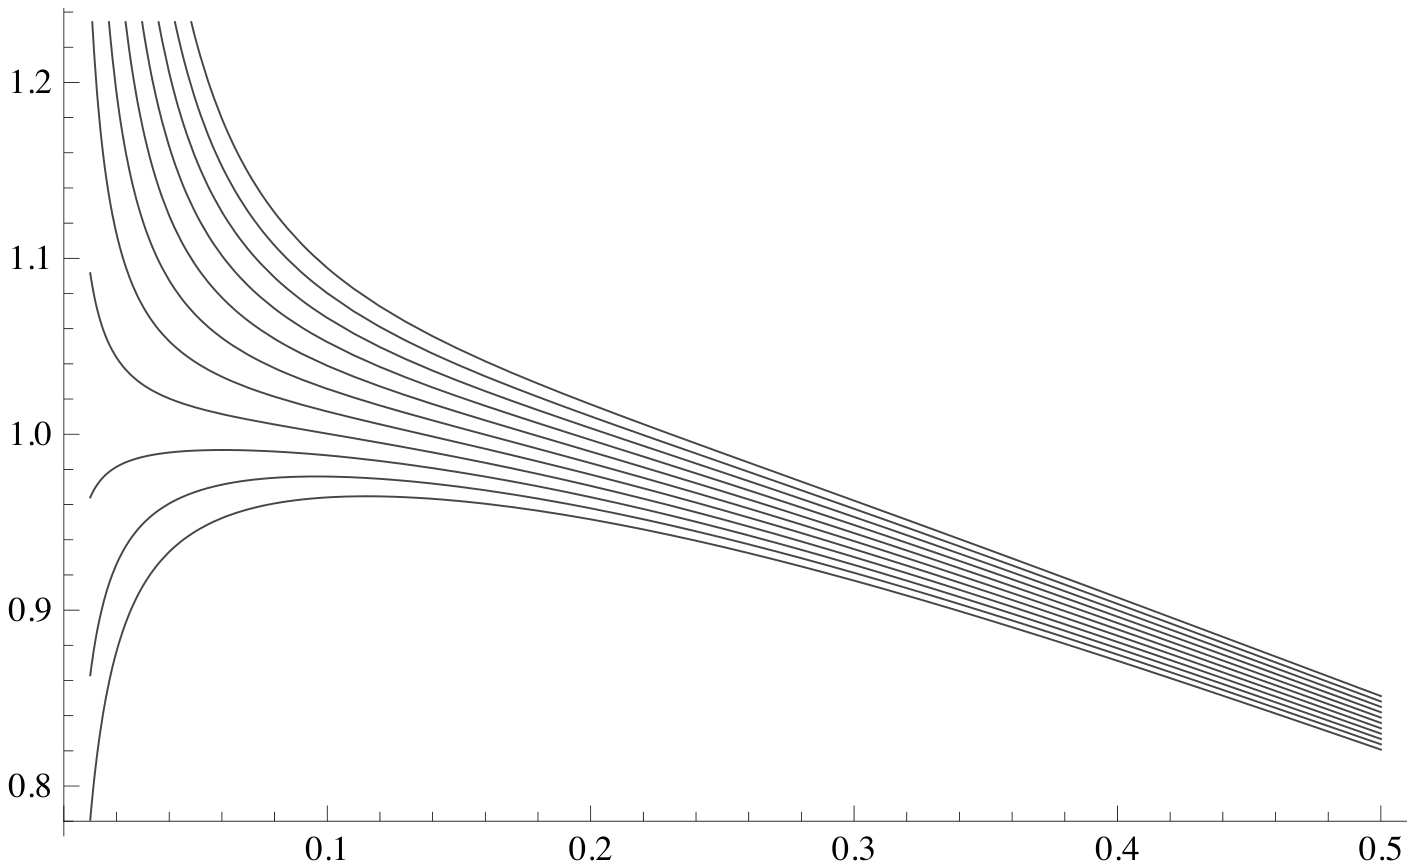
\includegraphics[width=3.5in]{figs/Fig29.png}
 \end{center}
\caption{\small  当 $\delta$ 跨过临界值变化时（取 $k=1$）的数值解。（原稿第 117 页）}
 \label{braidbo}
\end{figure}
   % 附录 C

% ---------------- 附录 D：术语对照表 ----------------
\newpage
% =====================================================================
%  glossary.tex —— 附录 D：英中术语对照表
% =====================================================================
\section{英中术语对照表}\label{app:glossary}

下表列出本译稿采用的术语译名，以便与中文文献对照。人名、理论名与数学专名（Jones、Khovanov、Nahm、oper 等）按学术惯例保留原文，不列入表中。

\begin{longtable}{p{0.20\textwidth}p{0.27\textwidth}p{0.20\textwidth}p{0.27\textwidth}}
\toprule
英文 & 中文 & 英文 & 中文 \\
\midrule
\endhead
gauge theory / gauge field & 规范场论 / 规范场 & electric-magnetic duality & 电磁对偶 \\
Jones polynomial & Jones 多项式 & knot invariant & 纽结不变量 \\
Khovanov homology & Khovanov 同调 & Chern-Simons theory & Chern-Simons 理论 \\
conformal field theory & 共形场论 & conformal block & 共形块 \\
Virasoro algebra & Virasoro 代数 & degenerate representation & 退化表示 \\
primary field & 初级场 & operator product expansion & 算符乘积展开 \\
anomaly & 反常 & holonomy & 和乐 \\
Wilson line/loop & Wilson 线/圈 & 't Hooft operator & 't Hooft 算符 \\
monopole & 磁单极子 & instanton & 瞬子 \\
supersymmetry & 超对称 & super Yang-Mills & 超 Yang-Mills \\
BPS state & BPS 态 & moduli space & 模空间 \\
Coulomb branch & 库仑分支 & Higgs branch & 希格斯分支 \\
self-dual / anti-self-dual & 自对偶 / 反自对偶 & Hodge star & Hodge 星号算子 \\
exterior derivative & 外微分 & connection & 联络 \\
curvature & 曲率 & bundle & 丛 \\
principal bundle & 主丛 & adjoint representation & 伴随表示 \\
Lie algebra & 李代数 & principal embedding & 主嵌入 \\
regular element & 正则元素 & maximal torus & 极大环面 \\
weight & 权 & highest weight & 最高权 \\
root & 根 & Weyl group & Weyl 群 \\
representation & 表示 & tensor product & 张量积 \\
braid group & 辫群 & braiding & 编织 \\
monodromy & 单值性 & monodromy defect & 单值性缺陷 \\
line defect & 线缺陷 & surface operator & 曲面算符 \\
partition function & 配分函数 & path integral & 路径积分 \\
saddle point & 鞍点 & Picard-Lefschetz theory & Picard-Lefschetz 理论 \\
thimble & 针（thimble） & steepest descent & 最速下降 \\
Stokes line/wall & Stokes 线/墙 & wall crossing & 穿墙 \\
superpotential & 超势 & $M$-theory & $M$ 理论 \\
brane & 膜 & fivebrane & 五膜 \\
D-brane & D 膜 & NS5-brane & NS5 膜 \\
gauge/gravity duality & 规范/引力对偶 & low energy effective & 低能有效 \\
geometric Langlands & 几何 Langlands & flat connection & 平坦联络 \\
Bethe ansatz & Bethe 拟设 & Gaudin model & Gaudin 模型 \\
KZ equation & KZ（Knizhnik-Zamolodchikov）方程 & WZW model & WZW 模型 \\
Liouville theory & Liouville 理论 & chiral algebra & 手征代数 \\
stress tensor & 应力张量 & central charge & 中心荷 \\
null state & 零态 & fusion & 融合 \\
intertwining operator & 交织算符 & Verma module & Verma 模 \\
universal enveloping algebra & 泛包络代数 & affine Lie algebra & 仿射李代数 \\
current algebra & 流代数 & highest weight module & 最高权模 \\
saddle-point approximation & 鞍点近似 & gradient flow & 梯度流 \\
critical point & 临界点 & Morse theory & Morse 理论 \\
homology & 同调 & cycle & 链（积分链） \\
Riemann surface & 黎曼面 & complex structure & 复结构 \\
holomorphic & 全纯 & meromorphic & 亚纯 \\
pole & 极点 & residue & 留数 \\
skein relation & 拆接关系 & Kauffman bracket & Kauffman 括号 \\
unknot & 平凡纽结 & crossing & 交叉 \\
strand & 股 & trivalent vertex & 三价顶点 \\
Seiberg-Witten & Seiberg-Witten & Hitchin moduli space & Hitchin 模空间 \\
spectral curve & 谱曲线 & ramification & 分支 \\
puncture & 穿刺点 & regular singularity & 正则奇点 \\
irregular singularity & 非正则奇点 & Stokes matrix & Stokes 矩阵 \\
Lefschetz fibration & Lefschetz 纤维化 & vanishing cycle & 消没链 \\
superspace & 超空间 & supercharge & 超荷 \\
Nekrasov partition function & Nekrasov 配分函数 & Seiberg duality & Seiberg 对偶 \\
orientifold & 定向折叠面 & orbifold & 轨道流形 \\
\bottomrule
\end{longtable}


% ---------------- 参考文献 ----------------
% 参考文献（保留英文原貌；条目与原文一致）

\begin{thebibliography}{99}


\bibitem{Jones}
V. F. R. Jones, ``A Polynomial Invariant For Links Via Von Neumann Algebras,'' Bull.
AMS {\bf{12}} (1985) 103.

\bibitem{Khovanov}
M. Khovanov, ``A Categorification Of The Jones Polynomial,'' Duke. Math. J. {\bf
101} (2000)
359-426.

\bibitem{GSV}
S. Gukov, A. S. Schwarz, and C. Vafa,
``Khovanov-Rozansky Homology And Topological Strings,''
Lett. Math. Phys. {\bf 74} (2005) 53-74, hep-th/0412243.

\bibitem{OV}
H. Ooguri and C. Vafa, ``Knot Invariants And Topological Strings,''  Nucl. Phys.
{\bf{B577}}
(2000) 419, hep-th/9912123.

\bibitem{LMV} 
J. M. F. Labastida, M. Mari\~no and C. Vafa, ``Knots, Links, and Branes at Large $N$,'''
JHEP 0011(2000) 007, hep-th/0010102.



\bibitem{NV}
A. Neitzke and C. Vafa, ``Topological Strings And Their Physical Applications,''  hep-th/0410178.

\bibitem{Ma}
M. Marin\~o,  {\it Chern-Simons Theory, Matrix Models, And Topological Strings} 
(Oxford University Press, 2005).


\bibitem{DGR}
N. M. Dunfield, S. Gukov, and J. Rasmussen, ``The Superpotential For Knot Homologies,''
Experiment. Math. {\bf 15} (2006) 129, arXiv:math/0505662.

\bibitem{DVV}
R. Dijkgraaf, C. Vafa, and E. Verlinde, ``$M$-Theory And A Topological String Duality,''
hep-th/0602087.

\bibitem{AY}
M. Aganagic and M. Yamazaki,  ``Open BPS Wall Crossing And $M$-Theory,'' Nucl. Phys.
{\bf B834} (2010) 258-272.

\bibitem{CNV} S. Cecotti, A. Neitzke, and C. Vafa, ``$R$-Twisting And 4d/2d Corresondence,''
arXiv:1006:3435.

\bibitem{ACDKV}
M. Aganagic, M. C. N. Cheng, R. Dijkgraaf, D. Krefl, and C. Vafa,
``Quantum Geometry Of Refined Topological Strings,'' arXiv:1105.0630.

\bibitem{AgS}
M. Aganagic and S. Shakirov, ``Knot Homology From Refined Chern-Simons Theory,''
to appear.

\bibitem{fiveknots}
E. Witten, ``Fivebranes And Knots,'' arXiv:1101.3216.

\bibitem{KW}
A. Kapustin and E. Witten, ``Electric-Magnetic Duality And The Geometric Langlands
Program,''  Commun. Numb. Th. Phys. {\bf 1} (2007) 1-236,
hep-th/0604151.


\bibitem{Krontwo}
P. B. Kronheimer, ``Instantons And The Geometry Of The Nilpotent Variety,''
J. Diff. Geom. {\bf 32} (1990) 473-490.


\bibitem{Haydys}
A. Haydys, ``Fukaya-Seidel Category And Gauge Theory,''
arXiv:1010.2353.


\bibitem{Kronheimer}
P. B. Kronheimer, MSc. thesis (Oxford University, 1986), unpublished.

\bibitem{gw}
D. Gaiotto and E. Witten, ``Supersymmetric Boundary Conditions In $\N=4$ Super
Yang-Mills Theory,'' arXiv:08042907.

\bibitem{Hitchin}
N. Hitchin, ``The Self-Duality Equations On A Riemann Surface,'' Proc. London Math. Soc.
(3) {\bf 55} (1987) 59-126.

\bibitem{Corlette}
K. Corlette,  ``Flat $G$-Bundles With Canonical Metrics,'' J. Diff. Geom. {\bf 28} (1988)
361-382.

\bibitem{Frenkel}
E. Frenkel, ``Gaudin Model And Opers,'' arXiv:math/0407524.

\bibitem{Teschner}
J. Teschner, ``Quantization Of The Hitchin Moduli Spaces, Liouville Theory,
And The Geometric Langlands Correspondence I,'' arXiv:1005:2846.

\bibitem{BF}
H. M. Babujian and R. Flume, ``Off-Shell Bethe Ansatz Equation
For Gaudin Magnets and Solutions Of Knizhnik-Zamolodchikov Equations,''
Mod. Phys. Lett. {\bf A9} (1994) 2029-2039.

\bibitem{FFR}
B. Feigin, E. Frenkel, and N. Reshetikin, ``Gaudin Model, Bethe Ansatz, and
Critical Level,'' Commun. Math. Phys. {\bf 166} (1994) 27-62.


\bibitem{TK}
A. Tsuchiya and Y. Kanie, ``Vertex Operators In Conformal Field Theory On
$\P^1$ And Monodromy Representations of Braid Group,'' Adv. Stud. Pure
Math. {\bf 16} 297-372.

\bibitem{KZ}
V. G. Knizhnik and A. B. Zamolodchikov, ``Current Algebra And
Wess-Zumino Model In Two-Dimensions,'' Nucl. Phys. {\bf B247} 83-103.

\bibitem{Ry}
L. G. Rybnikov, ``Argument Shift Method And Gaudin Model,'' Func. Anal. Appl. {\bf 40}
(2006) No. 3, math.RT/0606380.

\bibitem{FFT}
B. Feigin, E. Frenkel, and V. Toledano-Laredo,
``Gaudin Models With Irregular Singularities,'' arXiv:math/0612798,
and to appear.

\bibitem{FFRy}
B. Feigin, E. Frenkel, and L. Rybnikov, ``Opers With Irregular Singularity And Spectra Of The Shift of Argument
Subalgebra,'' arXiv:0712.1183.


\bibitem{BPZ}
A. A. Belavin,
A. M. Polyakov, and A. B. Zamolodchikov, ``Infinite Conformal Symmetry In Two-Dimensional
Quantum Field Theory,'' Nucl. Phys. {\bf B241} (1984) 333-380.

\bibitem{DF}
Vl. S. Dotsenko and V. A. Fateev, ``Conformal Algebra And Multipoint Correlation Functions in 2D Statistical Models,''
Nucl. Phys. {\bf B240}  (1984) 312-348.

\bibitem{Felder}
G. Felder, ``BRST Approach To Minimal Models,''  Nucl. Phys. {\bf B317} (1989) 215.

\bibitem{Lawrence}
R. J. Lawrence, ``Homological Representations Of The Hecke Algebra,'' Commun.
Math. Phys. {\bf 135} (1990) 141-191.

\bibitem{SV}
V. V. Schechtman and A. N. Varchenko, ``Arrangements of Hyperplanes And Lie Algebra
Homology,'' Invent. Math. {\bf 106}
(1991) 139.

\bibitem{G}
D.Gaiotto,  ``Asymptotically Free $\N=2$ Theories And Irregular Conformal Blocks,''
arXiv:0908.0307.

\bibitem{Miwa}
T. Miwa, ``Clifford Operators And Riemann's Monodormy Problem,'' Publ. Res. Inst. Math.
Sci. Kyoto {\bf 17} (1981) 665.

\bibitem{Moore}
G. W. Moore, ``Matrix Models Of 2-D Gravity And Isomonodromic Deformation,'' Prog. Theor.
Phys. Suppl. {\bf 102} (1990) 255-286.

\bibitem{hutchings}
M. Hutchings, ``Lecture Notes On Morse Homology (with an eye towards Floer theory and pseudoholomorphic curves),''
available at \url{math.berkeley.edu/~hutching/teach/276-2010/mfp.ps}.

\bibitem{Analytic}
E. Witten, ``Analytic Continuation Of Chern-Simons Theory,'' arXiv:1001.2933.

\bibitem{NewLook}
E. Witten, ``A New Look At The Path Integral Of Quantum Mechanics,''
arXiv:1009:6032.

\bibitem{Morse}
E. Witten, ``Supersymmetry And Morse Theory,''  J. Diff. Geom. {\bf 17} (1982) 661-692.

\bibitem{FLN}
E. Frenkel, A. Losev, and N. Nekrasov, ``Instantons Beyond Topological Theory, I,''
hep-th/0610149.

\bibitem{WittenJones}
E. Witten, ``Quantum Field Theory And The Jones Polynomial,'' Commun. Math. Phys. {\bf 121}
(1989) 351-399.

\bibitem{HVerlinde}
H. Verlinde, ``Conformal Field Theory, Two-Dimensional Gravity, and Quantization Of Teichmuller
Space,'' Nucl. Phys. {\bf B337} (1990) 652-680.

\bibitem{Bilal}
A. Bilal, ``$W$-Algebras From Chern-Simons Theory,'' Phys. Lett. {\bf B267} (1991) 487-496.

\bibitem{DeBoer}
J. de Boer and J. Goeree, 
``$W$ Gravity From Chern-Simons Theory,'' Nucl. Phys. {\bf B381} (1991)
329-359.




\bibitem{Ltwo}
R. Lawrence, ``The Homological Approach To Higher Representations''
(Harvard preprint, 1990), available at \url{http://www.ma.huji.ac.il/~ruthel/}.

\bibitem{Kauffman}
L. H. Kauffman, {\it Knots And Physics} (World Scientific, 1991).

\bibitem{KauffmanTwo}
L. H. Kauffman, ``Map Coloring, $q$-Deformed Spin Networks, and Turaev-Viro Invariants
For 3-Manifolds,'' Int. J. Mod. Phys. {\bf B6} (1992) 1765-1794.

\bibitem{Vertex}
E. Witten, ``Gauge Theories, Vertex Models, and Quantum Groups,'' Nucl. Phys. {\bf B330} (1990)
285-346.

\bibitem{AS}
S. Albeverio and A. N. Sengupta, ``A Mathematical
Construction Of The Non-Abelian Chern-Simons Functional Integral,''
Commun. Math. Phys. {\bf 186} (1997) 563-579.

\bibitem{Hahn}
A. Hahn, ``The Wilson Loop Observables Of Chern-Simons On $\R^3$ In Axial Gauge,''
Commun. Math. Phys. {\bf 248} (2004) 467-499.



\bibitem{Wetering}
J. F. W. H. van de Wetering, ``Knot Invariants And Universal $R$-Matrices From Perturbative
Chern-Simons Theory In The Almost Axial Gauge,'' Nucl. Phys. {\bf B379} (1992) 172-198.


\bibitem{FK}
J. Fr\"ohlich and C. King, ``The Chern-Simons Theory And Knot Polynomials,'' Commun. Math. Phys.
{\bf 126} (1989) 167-199.

\bibitem{AH}
M. F. Atiyah and N. Hitchin,  {\it The Geometry And Dynamics Of Magnetic Monopoles}
(Princeton University Press, 1988).

\bibitem{Hurtubise}
J. Hurtubise, ``Monopoles And Rational Maps: A Note On A Theorem
of Donaldson,''  Commun. Math. Phys. {\bf 100} (1985) 191-196.

\bibitem{GHR}
  S.~J.~Gates, C.~M.~Hull and M.~Rocek,
  ``Twisted Multiplets And New Supersymmetric Nonlinear Sigma Models,''
  Nucl.\ Phys.\   {\bf B248} (1984) 157.

\bibitem{diac}
 D.~E.~Diaconescu,
  ``D-Branes, Monopoles and Nahm Equations,''
  Nucl.\ Phys.\  B {\bf 503} (1997) 220, arXiv:hep-th/9608163.


\bibitem{BVJ}
 M.~Bershadsky, A.~Johansen, V.~Sadov, C.~Vafa,
  ``Topological Reduction of 4-d SYM to 2-d Sigma Models,''
  Nucl.\ Phys.\  {\bf B448 } (1995)  166-186,
  hep-th/9501096.

\bibitem{HM}
J.~A.~Harvey, G.~W.~Moore, A.~Strominger,
  ``Reducing $S$ Duality to $T$ Duality,
  Phys.\ Rev.\  {\bf D52 } (1995)  7161-7167
  hep-th/9501022.

\bibitem{Frenkeltwo}
 E.~Frenkel,
  ``Lectures on the Langlands Program and Conformal Field Theory,''
  hep-th/0512172.

\bibitem{NW}
N.~Nekrasov and E.~Witten,
  ``The Omega Deformation, Branes, Integrability, and Liouville Theory,''
  JHEP {\bf 1009 } (2010)  092,
  arXiv:1002.0888 [hep-th].

\bibitem{AGT}
L. F. Alday, D. Gaiotto, and Y. Tachikawa, ``Liouville Correlation Functions From Four-Dimensional
Gauge Theories,'' arXiv:0906.3219.

\bibitem{NS}
 N.~A.~Nekrasov and S.~L.~Shatashvili,
  ``Quantum Integrability and Supersymmetric Vacua,''
  Prog.\ Theor.\ Phys.\ Suppl.\  {\bf 177 } (2009)  105-119,
  arXiv:0901.4748 [hep-th].


\bibitem{NStwo}
  N.~Nekrasov, A.~Rosly, and S.~Shatashvili,
  ``Darboux Coordinates, Yang-Yang Functional, and Gauge Theory,''
  arXiv:1103.3919 [hep-th].

\bibitem{Simpson}
C. Simpson, ``Harmonic Bundles On Noncompact Curves,'' J. Am. Math. Soc. {\bf 3} (1990)
713-770.

\bibitem{GuW}
S. Gukov and E. Witten, ``Gauge Theory, Ramification, And The Geometric Langlands
Program,'' hep-th/0612073.


\bibitem{Mikhaylov}
V. Mikhaylov, to appear.

\bibitem{GuWtwo}
S. Gukov and E. Witten, ``Branes And Quantization,''  arXiv:0809.0305.

\bibitem{LiTam}
P. Li and L.-F. Tam, ``The Heat Equation And Harmonic Maps Of Complete Manifolds,''
Invent. Math. {\bf 105} (1991) 1-46.

\end{thebibliography}


\end{document}
